\documentclass[]{book}
\usepackage{lmodern}
\usepackage{amssymb,amsmath}
\usepackage{ifxetex,ifluatex}
\usepackage{fixltx2e} % provides \textsubscript
\ifnum 0\ifxetex 1\fi\ifluatex 1\fi=0 % if pdftex
  \usepackage[T1]{fontenc}
  \usepackage[utf8]{inputenc}
\else % if luatex or xelatex
  \ifxetex
    \usepackage{mathspec}
  \else
    \usepackage{fontspec}
  \fi
  \defaultfontfeatures{Ligatures=TeX,Scale=MatchLowercase}
\fi
% use upquote if available, for straight quotes in verbatim environments
\IfFileExists{upquote.sty}{\usepackage{upquote}}{}
% use microtype if available
\IfFileExists{microtype.sty}{%
\usepackage{microtype}
\UseMicrotypeSet[protrusion]{basicmath} % disable protrusion for tt fonts
}{}
\usepackage[margin=1in]{geometry}
\usepackage{hyperref}
\hypersetup{unicode=true,
            pdftitle={Modelling Criminological Data LAWS20452},
            pdfauthor={Juanjo Medina and Reka Solymosi},
            pdfborder={0 0 0},
            breaklinks=true}
\urlstyle{same}  % don't use monospace font for urls
\usepackage{natbib}
\bibliographystyle{apalike}
\usepackage{color}
\usepackage{fancyvrb}
\newcommand{\VerbBar}{|}
\newcommand{\VERB}{\Verb[commandchars=\\\{\}]}
\DefineVerbatimEnvironment{Highlighting}{Verbatim}{commandchars=\\\{\}}
% Add ',fontsize=\small' for more characters per line
\usepackage{framed}
\definecolor{shadecolor}{RGB}{248,248,248}
\newenvironment{Shaded}{\begin{snugshade}}{\end{snugshade}}
\newcommand{\AlertTok}[1]{\textcolor[rgb]{0.94,0.16,0.16}{#1}}
\newcommand{\AnnotationTok}[1]{\textcolor[rgb]{0.56,0.35,0.01}{\textbf{\textit{#1}}}}
\newcommand{\AttributeTok}[1]{\textcolor[rgb]{0.77,0.63,0.00}{#1}}
\newcommand{\BaseNTok}[1]{\textcolor[rgb]{0.00,0.00,0.81}{#1}}
\newcommand{\BuiltInTok}[1]{#1}
\newcommand{\CharTok}[1]{\textcolor[rgb]{0.31,0.60,0.02}{#1}}
\newcommand{\CommentTok}[1]{\textcolor[rgb]{0.56,0.35,0.01}{\textit{#1}}}
\newcommand{\CommentVarTok}[1]{\textcolor[rgb]{0.56,0.35,0.01}{\textbf{\textit{#1}}}}
\newcommand{\ConstantTok}[1]{\textcolor[rgb]{0.00,0.00,0.00}{#1}}
\newcommand{\ControlFlowTok}[1]{\textcolor[rgb]{0.13,0.29,0.53}{\textbf{#1}}}
\newcommand{\DataTypeTok}[1]{\textcolor[rgb]{0.13,0.29,0.53}{#1}}
\newcommand{\DecValTok}[1]{\textcolor[rgb]{0.00,0.00,0.81}{#1}}
\newcommand{\DocumentationTok}[1]{\textcolor[rgb]{0.56,0.35,0.01}{\textbf{\textit{#1}}}}
\newcommand{\ErrorTok}[1]{\textcolor[rgb]{0.64,0.00,0.00}{\textbf{#1}}}
\newcommand{\ExtensionTok}[1]{#1}
\newcommand{\FloatTok}[1]{\textcolor[rgb]{0.00,0.00,0.81}{#1}}
\newcommand{\FunctionTok}[1]{\textcolor[rgb]{0.00,0.00,0.00}{#1}}
\newcommand{\ImportTok}[1]{#1}
\newcommand{\InformationTok}[1]{\textcolor[rgb]{0.56,0.35,0.01}{\textbf{\textit{#1}}}}
\newcommand{\KeywordTok}[1]{\textcolor[rgb]{0.13,0.29,0.53}{\textbf{#1}}}
\newcommand{\NormalTok}[1]{#1}
\newcommand{\OperatorTok}[1]{\textcolor[rgb]{0.81,0.36,0.00}{\textbf{#1}}}
\newcommand{\OtherTok}[1]{\textcolor[rgb]{0.56,0.35,0.01}{#1}}
\newcommand{\PreprocessorTok}[1]{\textcolor[rgb]{0.56,0.35,0.01}{\textit{#1}}}
\newcommand{\RegionMarkerTok}[1]{#1}
\newcommand{\SpecialCharTok}[1]{\textcolor[rgb]{0.00,0.00,0.00}{#1}}
\newcommand{\SpecialStringTok}[1]{\textcolor[rgb]{0.31,0.60,0.02}{#1}}
\newcommand{\StringTok}[1]{\textcolor[rgb]{0.31,0.60,0.02}{#1}}
\newcommand{\VariableTok}[1]{\textcolor[rgb]{0.00,0.00,0.00}{#1}}
\newcommand{\VerbatimStringTok}[1]{\textcolor[rgb]{0.31,0.60,0.02}{#1}}
\newcommand{\WarningTok}[1]{\textcolor[rgb]{0.56,0.35,0.01}{\textbf{\textit{#1}}}}
\usepackage{longtable,booktabs}
\usepackage{graphicx,grffile}
\makeatletter
\def\maxwidth{\ifdim\Gin@nat@width>\linewidth\linewidth\else\Gin@nat@width\fi}
\def\maxheight{\ifdim\Gin@nat@height>\textheight\textheight\else\Gin@nat@height\fi}
\makeatother
% Scale images if necessary, so that they will not overflow the page
% margins by default, and it is still possible to overwrite the defaults
% using explicit options in \includegraphics[width, height, ...]{}
\setkeys{Gin}{width=\maxwidth,height=\maxheight,keepaspectratio}
\IfFileExists{parskip.sty}{%
\usepackage{parskip}
}{% else
\setlength{\parindent}{0pt}
\setlength{\parskip}{6pt plus 2pt minus 1pt}
}
\setlength{\emergencystretch}{3em}  % prevent overfull lines
\providecommand{\tightlist}{%
  \setlength{\itemsep}{0pt}\setlength{\parskip}{0pt}}
\setcounter{secnumdepth}{5}
% Redefines (sub)paragraphs to behave more like sections
\ifx\paragraph\undefined\else
\let\oldparagraph\paragraph
\renewcommand{\paragraph}[1]{\oldparagraph{#1}\mbox{}}
\fi
\ifx\subparagraph\undefined\else
\let\oldsubparagraph\subparagraph
\renewcommand{\subparagraph}[1]{\oldsubparagraph{#1}\mbox{}}
\fi

%%% Use protect on footnotes to avoid problems with footnotes in titles
\let\rmarkdownfootnote\footnote%
\def\footnote{\protect\rmarkdownfootnote}

%%% Change title format to be more compact
\usepackage{titling}

% Create subtitle command for use in maketitle
\newcommand{\subtitle}[1]{
  \posttitle{
    \begin{center}\large#1\end{center}
    }
}

\setlength{\droptitle}{-2em}

  \title{Modelling Criminological Data LAWS20452}
    \pretitle{\vspace{\droptitle}\centering\huge}
  \posttitle{\par}
    \author{Juanjo Medina and Reka Solymosi}
    \preauthor{\centering\large\emph}
  \postauthor{\par}
      \predate{\centering\large\emph}
  \postdate{\par}
    \date{2019-01-29}

\usepackage{booktabs}

\usepackage{amsthm}
\newtheorem{theorem}{Theorem}[chapter]
\newtheorem{lemma}{Lemma}[chapter]
\theoremstyle{definition}
\newtheorem{definition}{Definition}[chapter]
\newtheorem{corollary}{Corollary}[chapter]
\newtheorem{proposition}{Proposition}[chapter]
\theoremstyle{definition}
\newtheorem{example}{Example}[chapter]
\theoremstyle{definition}
\newtheorem{exercise}{Exercise}[chapter]
\theoremstyle{remark}
\newtheorem*{remark}{Remark}
\newtheorem*{solution}{Solution}
\begin{document}
\maketitle

{
\setcounter{tocdepth}{1}
\tableofcontents
}
\hypertarget{preface}{%
\chapter*{Preface}\label{preface}}
\addcontentsline{toc}{chapter}{Preface}

This is the main text you will be using during the labs for the module
\emph{Modelling Criminological Data}. Every week you will have to use
these materials during the lab sessions. The idea is that you read this
book and try to run the code we provide in your own machine. Along the
way you will see you have to complete a series of exercises to check
that you are correctly understanding the materials that we introduce. We
hope you find these materials useful. They are a work in process, so
please if you have any suggestions please don't hesitate to get in touch
via
\href{mailto:juanjo.medina@manchester.ac.uk}{\nolinkurl{juanjo.medina@manchester.ac.uk}}.

\#A first lesson about R (Week 1)

\#\#Install R \& RStudio

We recommend that you use your own laptops for this course. This way you
get used to working in an environment which you will continue to use
after this semester. However, our lab sessions will be held in computer
clusters in case you do not have access to a laptop (or something goes
wrong\ldots{}).

You \emph{don't need to install the software in the computers available
in the clusters}, because it is already there. Beware though, the
installation may vary a bit across different computer clusters in the
University. This, on itself, is another good reason to use your own
laptops -for it will provide you with a more stable environment. If you
have not already, then please download and install R and R Studio onto
your laptops. Otherwise use the cluster machines.

\begin{itemize}
\tightlist
\item
  click \href{https://www.youtube.com/watch?v=eD07NznguA4}{here} for
  instructions using Windows or
\item
  \href{https://www.youtube.com/watch?v=cX532N_XLIs\&list=PLqzoL9-eJTNDw71zWePXyHx3_cm_fMP8S}{here}
  for instructions using a Mac.
\end{itemize}

\#\#Open up and explore RStudio

In this session we will focus in developing basic familiarity with R
Studio. You can use R without using R Studio, but R Studio is an app
that makes it easier to work with R.

R Studio is what we call an IDE, an \textbf{integrated development
environment}. It is a fancy way of saying that it is a cool interface
designed to write programming code. Every time you open up R Studio you
are in fact starting a R session. R Studio automatically runs R in the
background. We will be interacting with R in this course unit via R
Studio.

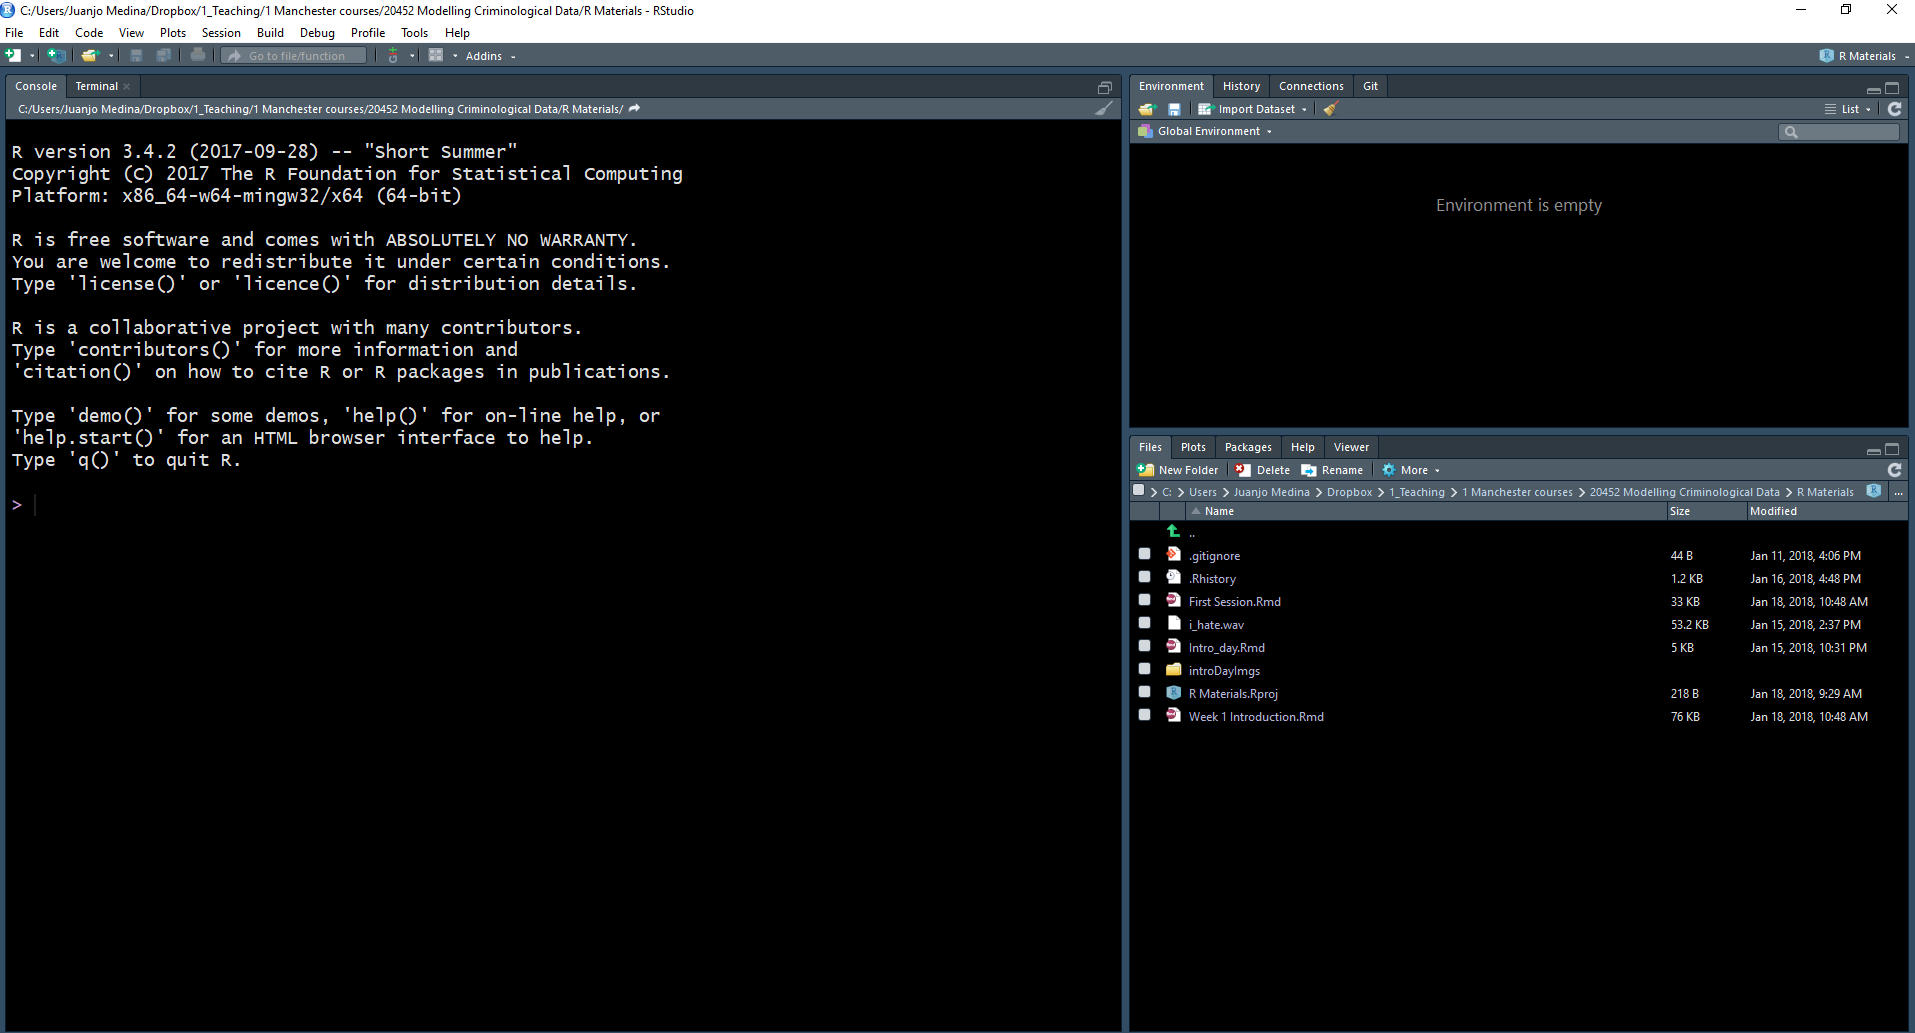
\includegraphics{imgs/rstudio.PNG}

When you first open R Studio, you will see (as in the image above) that
there are 3 main windows. The bigger one to your left is the console. If
you read the text in the console you will see that R Studio is indeed
opening R and you can see what version of R you are running. Depending
on whether you are using the cluster machines or your own installation
this may vary, but don't worry too much about it. R is constantly being
updated.

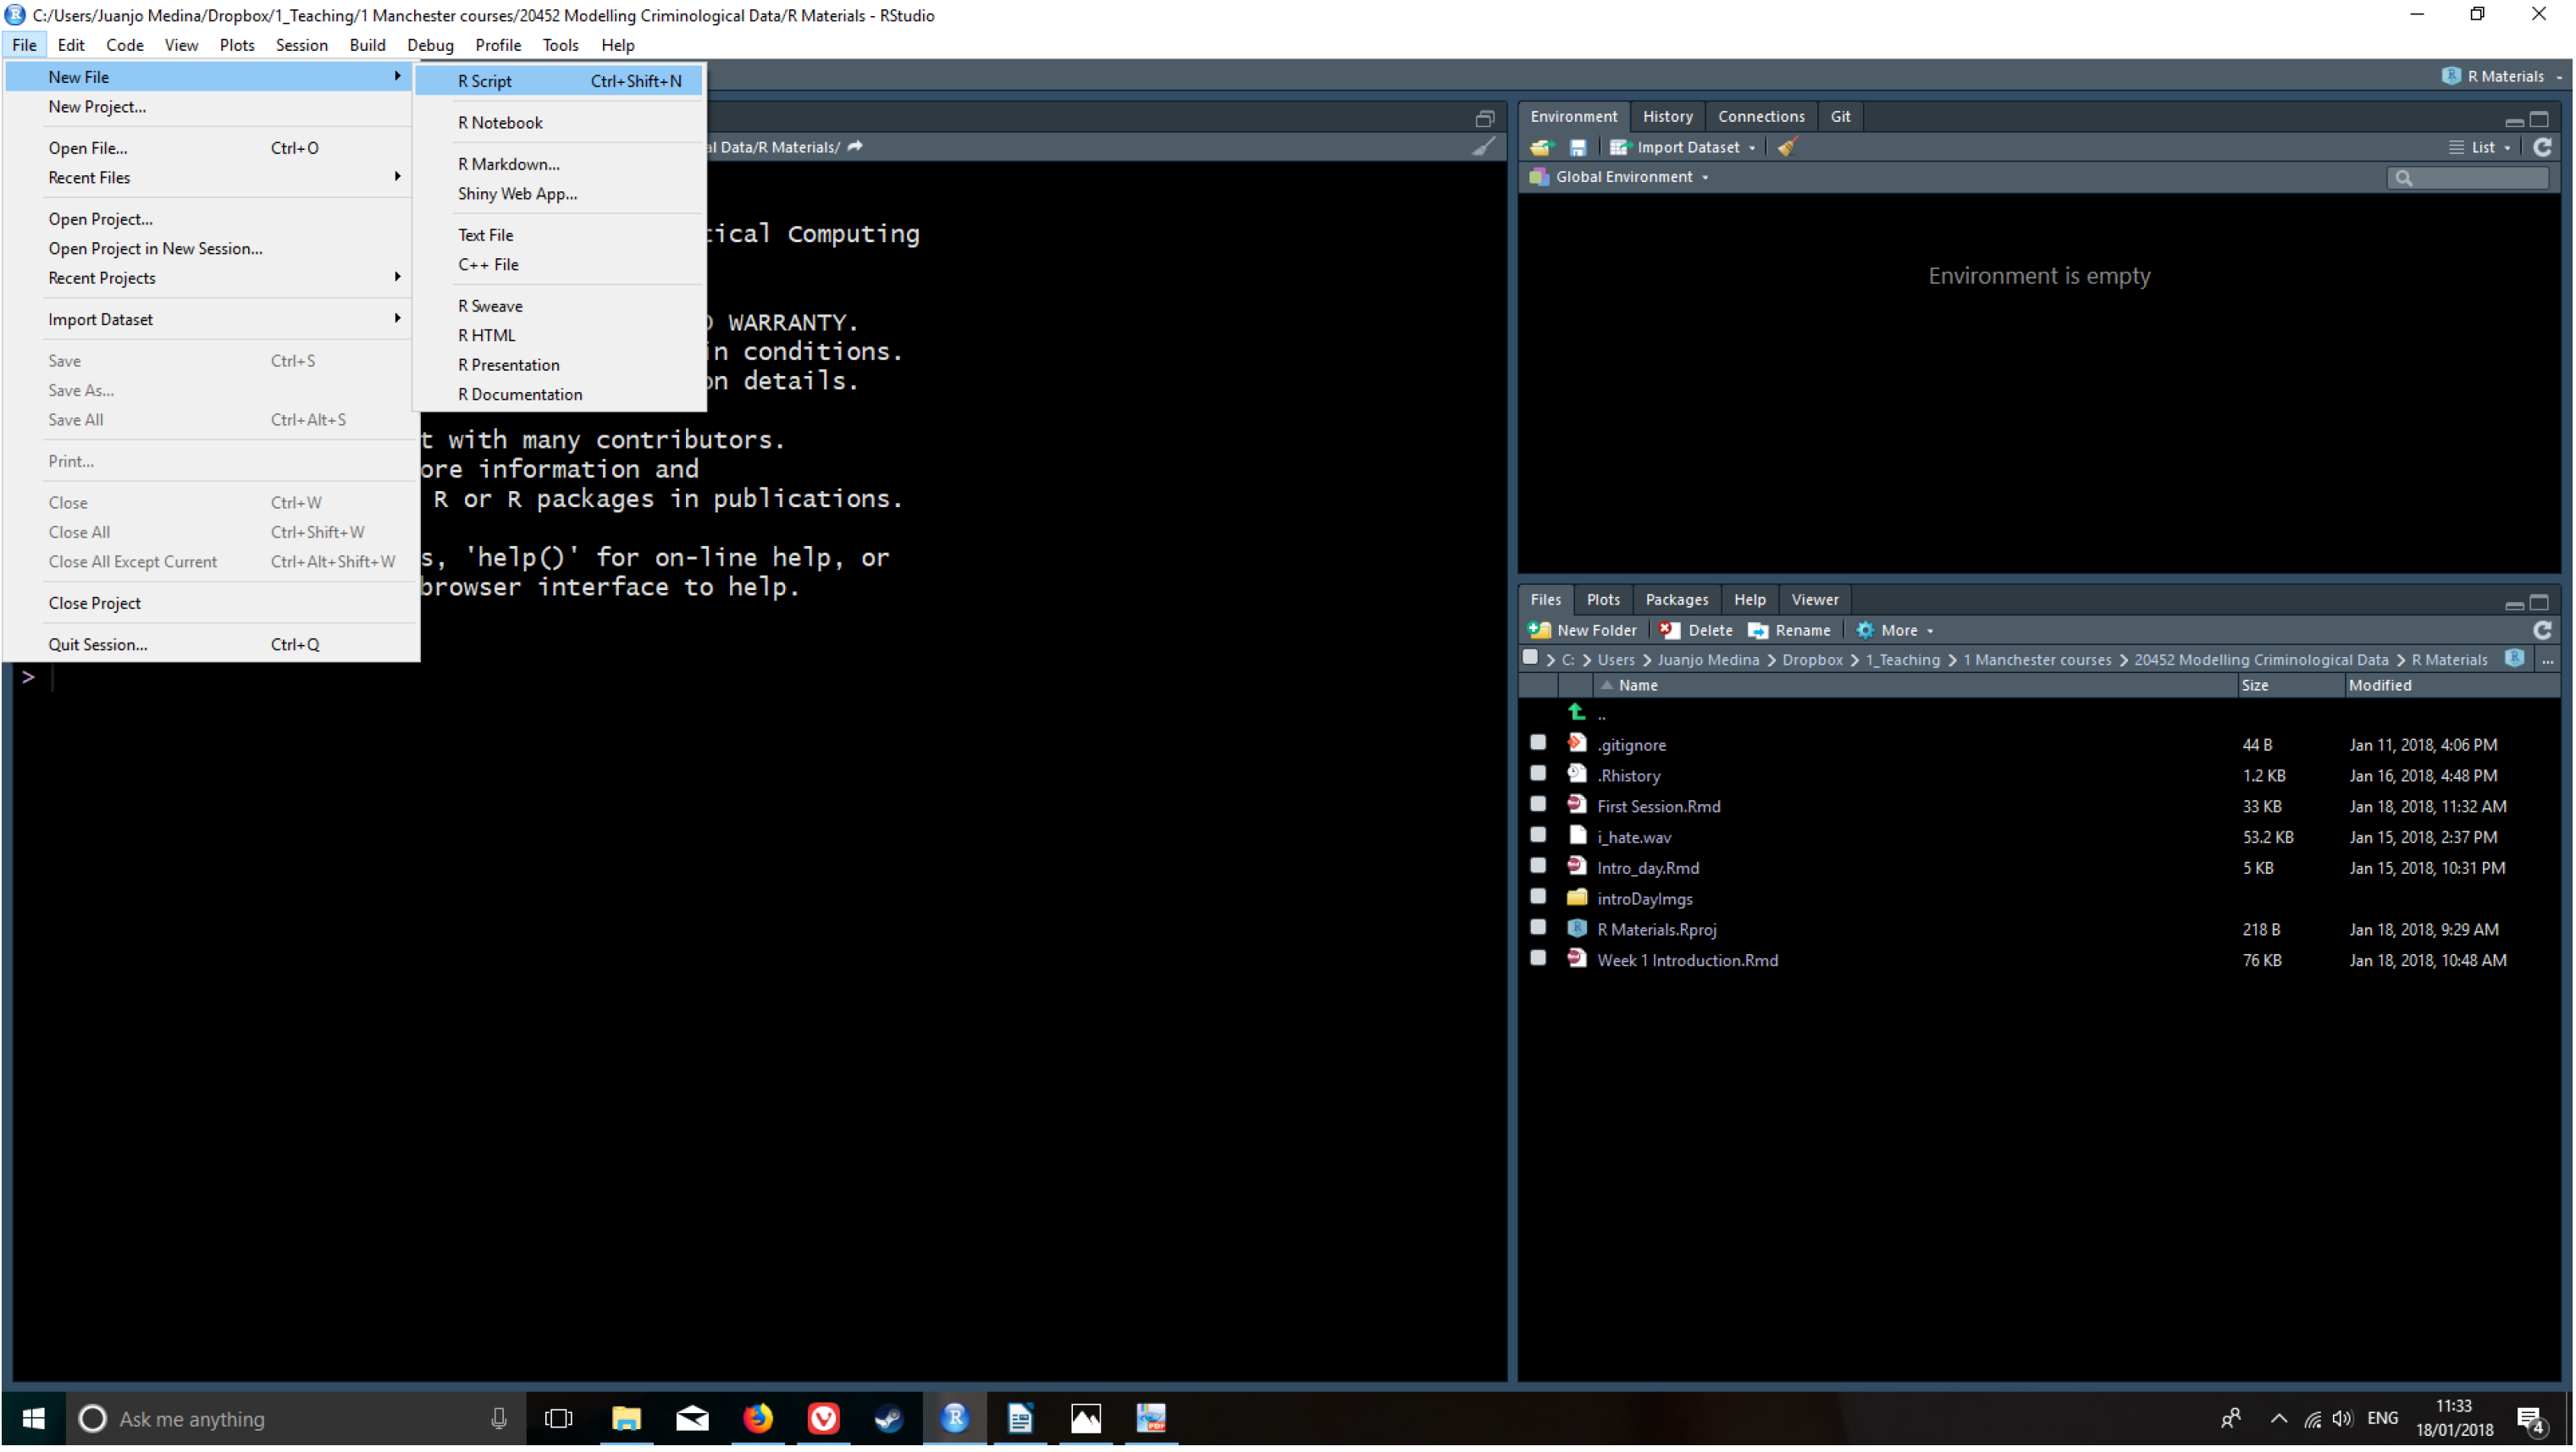
\includegraphics{imgs/openscript.png}

The view in R Studio is structured so that you have 4 open windows in a
regular session. Click in the \emph{File} drop down Menu, select
\emph{New File}, then \emph{R Script}. You will now see the 4 window
areas in display. On each of these areas you can shift between different
views and panels. You can also use your mouse to re-size the different
windows if that is convenient.

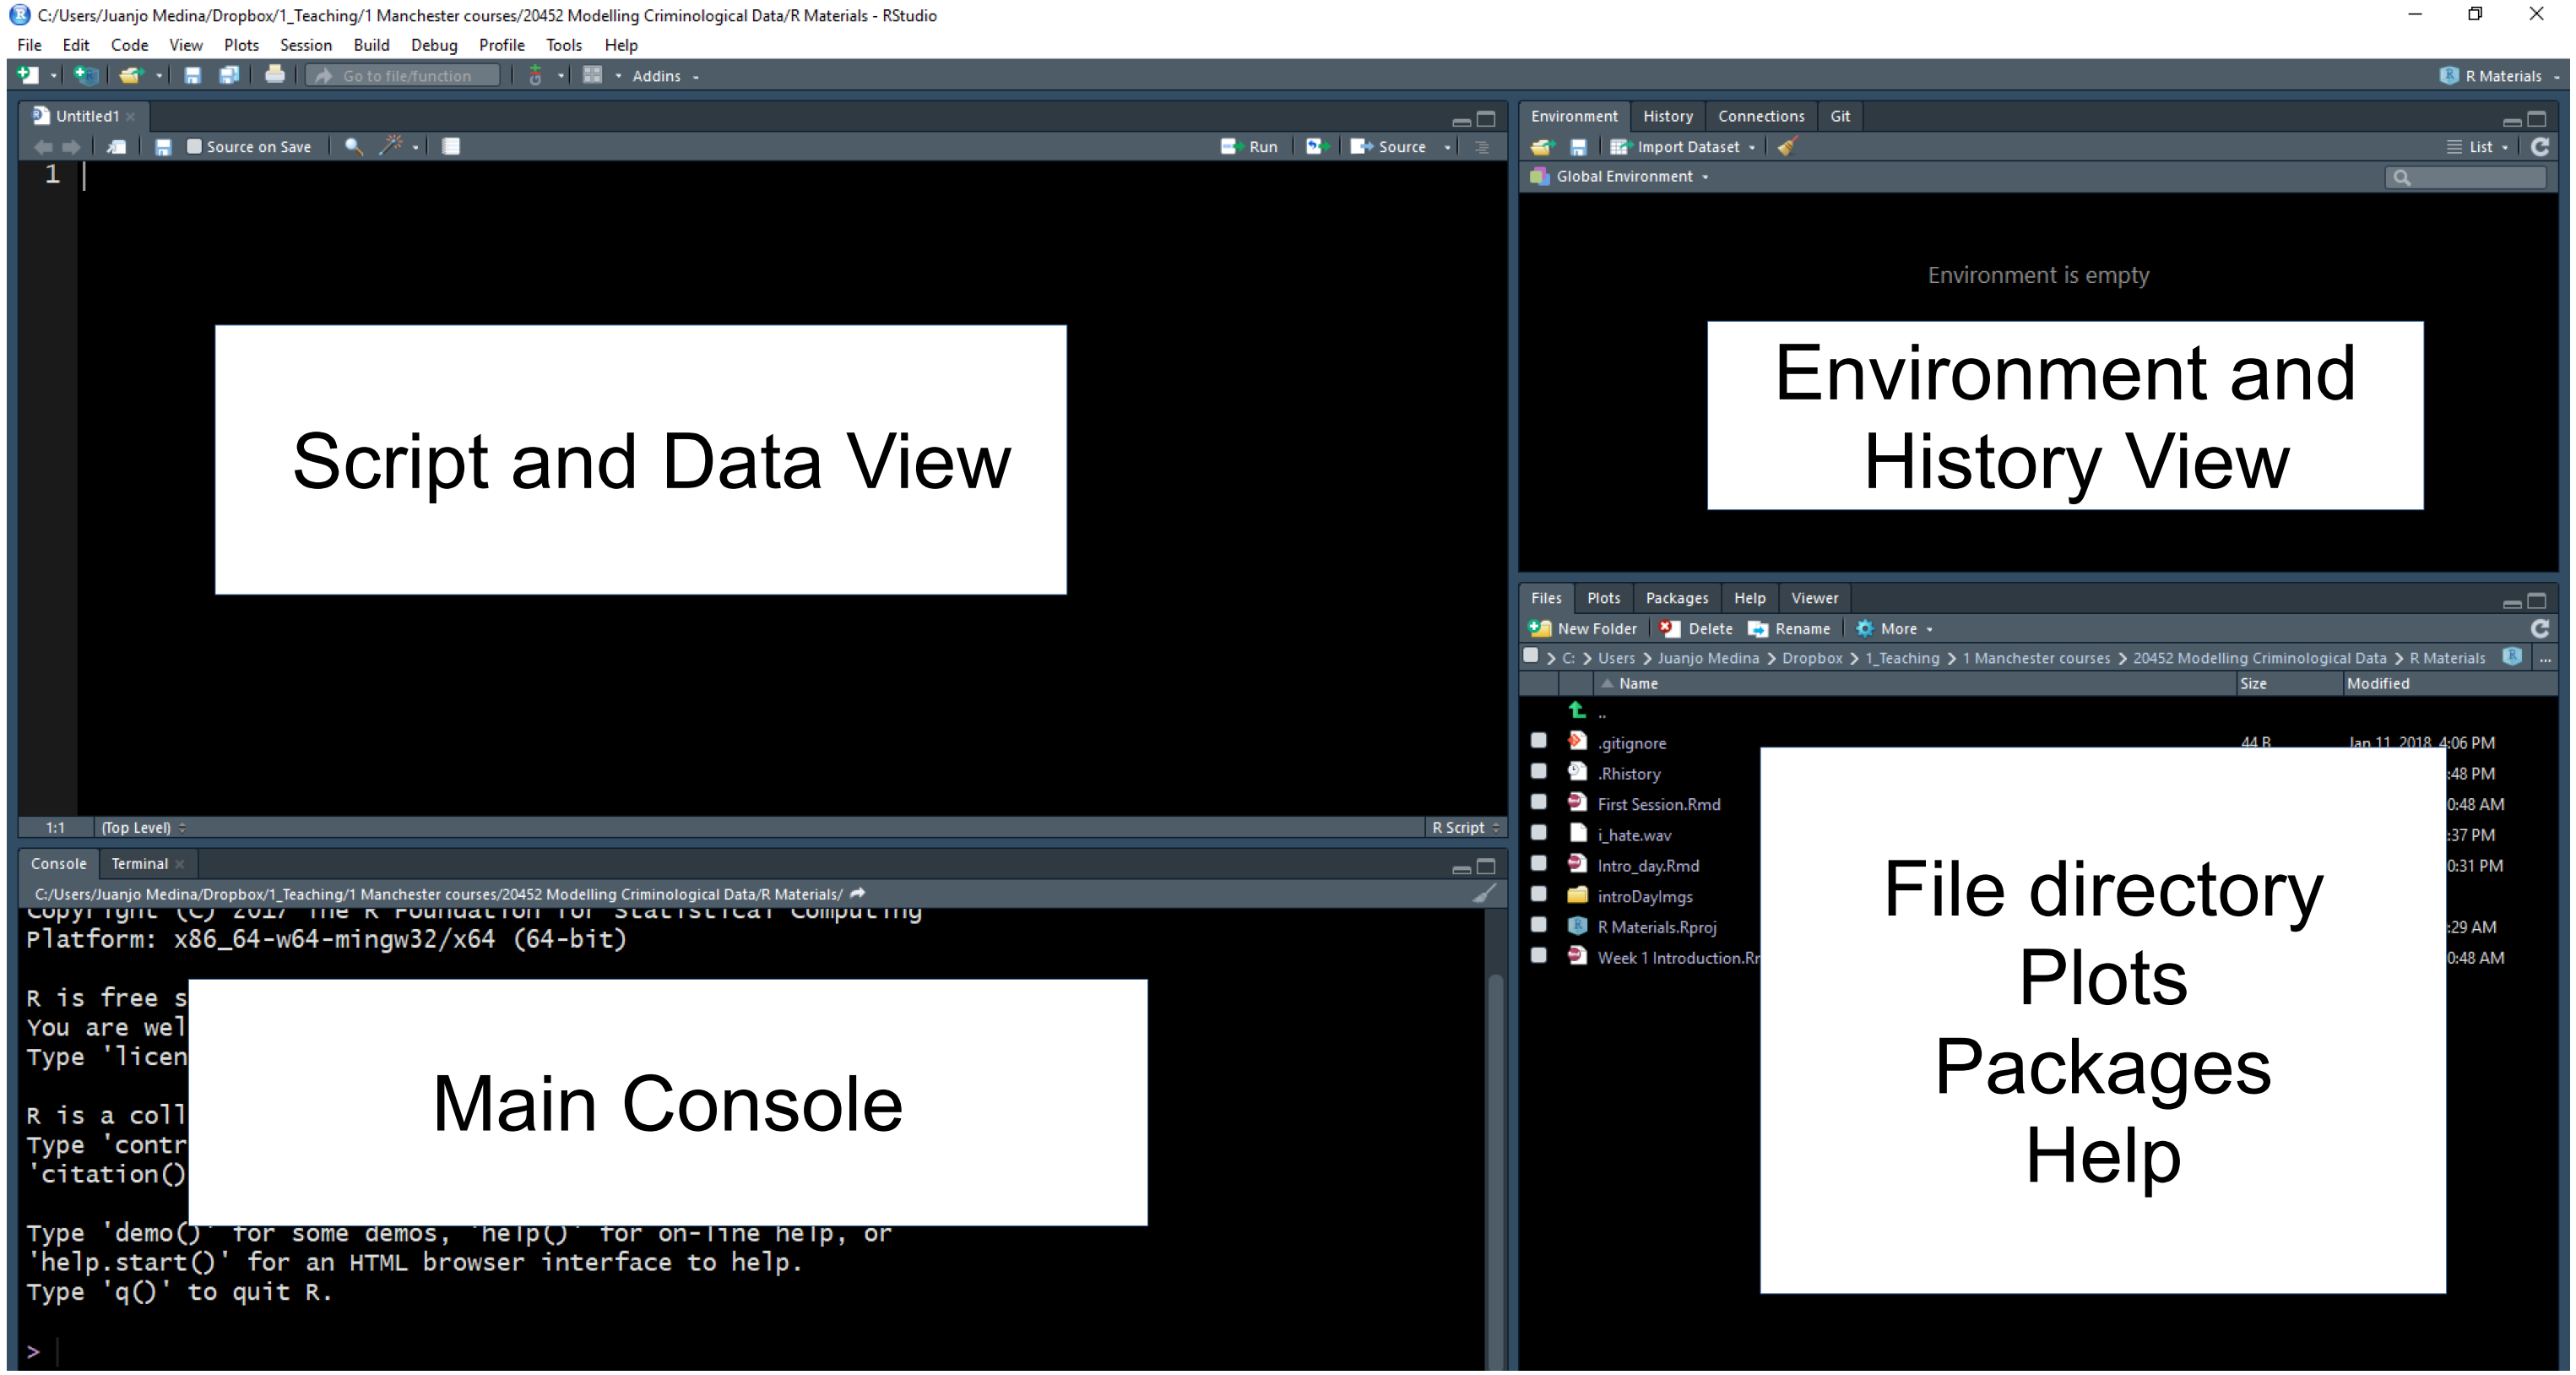
\includegraphics{imgs/the4views.png}

Look for example at the bottom right area. Within this area you can see
that there are different tabs, which are associated with different
views. You can see in the tabs in this section that there are different
views available: \emph{Files}, \emph{Plots}, \emph{Packages},
\emph{Help}, and \emph{Viewer}. The \textbf{Files} allow you to see the
files in the physical directory that is currently set up as your working
environment. You can think of it like a window in Windows Explorer that
lets you see the content of a folder.

In the \textbf{plots} panel you will see any data visualisations or
graphical displays of data that you produce. We haven't yet produced
any, so it is empty at the moment. If you click in \textbf{packages} you
will see the packages that are currently available in your installation.
What is a ``package'' in this context?

You can think of R as a Lego monster. You can make the monster scarier
and more powerful by adding new bits to it. Packages are those bits.
They are modules that expand what R can do. There are thousands of them.
Which is pretty cool!!! R can do many more things than Excel. That is
down to the fact that researchers all over the world write packages that
continuously expand the functionality of R. You can think of a package
as another drop down menu that gets added to you menu tab with loads of
new options for doing fancy stuff, only they are not really drop down
menus. You need to access their added functionality via programming
code. So yeah, R is like Excel or SPSS only with over 10,000 ``drop down
menus.'' And all for free.

The other really useful panel in this part of the screen is the
\textbf{Help} viewer. Here you can access the documentation for the
various packages that make up R. Learning how to use this documentation
will be essential if you want to be able to get the most from R.

In the diagonally opposite corner, the top left, you should now have an
open script window. The \textbf{script} is where you write your
programming code. A script is nothing but a text file with some code on
it. Unlike other programs for data analysis you may have used in the
past (Excel, SPSS), you need to interact with R by means of writing down
instructions and asking R to evaluate those instructions. R is an
\emph{interpreted} programming language: you write instructions (code)
that the R engine has to interpret in order to do something. And all the
instructions we write can and should be saved in a script, so that you
can return later to what you did.

One of the key advantages of doing data analysis this way - with code
versus with a point and click interface like Excel or SPSS is that you
are producing a written record of every step you take in the analysis.
First time around it will take you time to write these instructions, it
may be slower than pointing and clicking. And unlike with pointing and
clicking you need to know the ``words'' and ``grammar'' of this
language.

Luckily you don't need to memorise or know all these words. As with any
language the more you practice it, the easier it will become. More often
than not you will be doing a lot of cutting and pasting from chunks of
code we will give you. But we will also expect you to develop a basic
understanding of what these bits of code do. It is a bit like cooking.
At first you will just follow recipes as they are given to you, but as
you become more comfortable in your ``kitchen'' you will feel more
comfortable experimenting.

The advantage of doing analysis this way is that once you have written
your instructions and saved them in a file, you will be able to share it
with others and run it every time you want in a matter of seconds. This
creates a \emph{reproducible} record of your analysis: something that
your collaborators or someone else anywhere (including your future self,
the one that will have forgotten how to do the stuff) could run and get
the same results than you did at some point earlier. This makes science
more transparent and transparency brings with it many advantages. For
example, it makes your research more trustworthy. Don't underestimate
how critical this is. \textbf{Reproducibility} is becoming a key
criteria to assess good quality research. And tools like R allow us to
enhance it. You may want to read more about reproducible research
\href{http://theconversation.com/the-science-reproducibility-crisis-and-what-can-be-done-about-it-74198}{here}.

\#\#Customising the RStudio look

R Studio allows you to customise the way it looks. Working with white
backgrounds is not generally a good idea if you care about your
eyesight. If you don't want to end up with dry eyes not only it is good
you follow the 20-20-20 rule (every 20 minutes look for 20 seconds to an
object located 20 feet away from you), but it may also be a good idea to
use more eye friendly screen displays.

Click in the \emph{Tools} menu and select \emph{Global options}. This
will open up a pop up window with various options. Select
\emph{Appearance}. In this section you can change the font type and
size, but also the kind of theme background that R will use in the
various windows. I suffer from poor sight, so I often increase the font
type. I also use the \emph{Tomorrow Night Bright} theme to prevent my
eyes to go too dry from the effort of reading a lightened screen, but
you may prefer a different one. You can preview them and then click
apply to select the one you like. This will not change your results or
analysis. This is just something you may want to do in order to make
things look better and healthier for your.

\#\#Getting organised: R Projects

We finished the previous section talking about sharing your analytic
code. Let's face it. You would not bring a new partner or somebody that
you want to impress to your place before tidying a little bit first,
wouldn't you? In the same way, if you know you may have to share your
code, if you know you may have guests, you may want to keep your
analysis, data, and results tidy. R Studio helps a little bit with that.
R Studio helps with this by virtue of something called \textbf{R
Projects}.

Technically, a R Studio project is just a directory with the name of the
project, and a few files and folders created by R Studio for internal
purposes. This is where you should hold your scripts, your data, and
reports. You can manage this folder with your own operating system
manager (eg., Windows Explorer) or through the R Studio file manager
(that you access in the bottom right corner set of windows in R Studio).

When a project is reopened, R Studio opens every file and data view that
was open when the project was closed last time around. Let's learn how
to create a project. Go to the \emph{File} drown menu and select
\emph{New Project}.

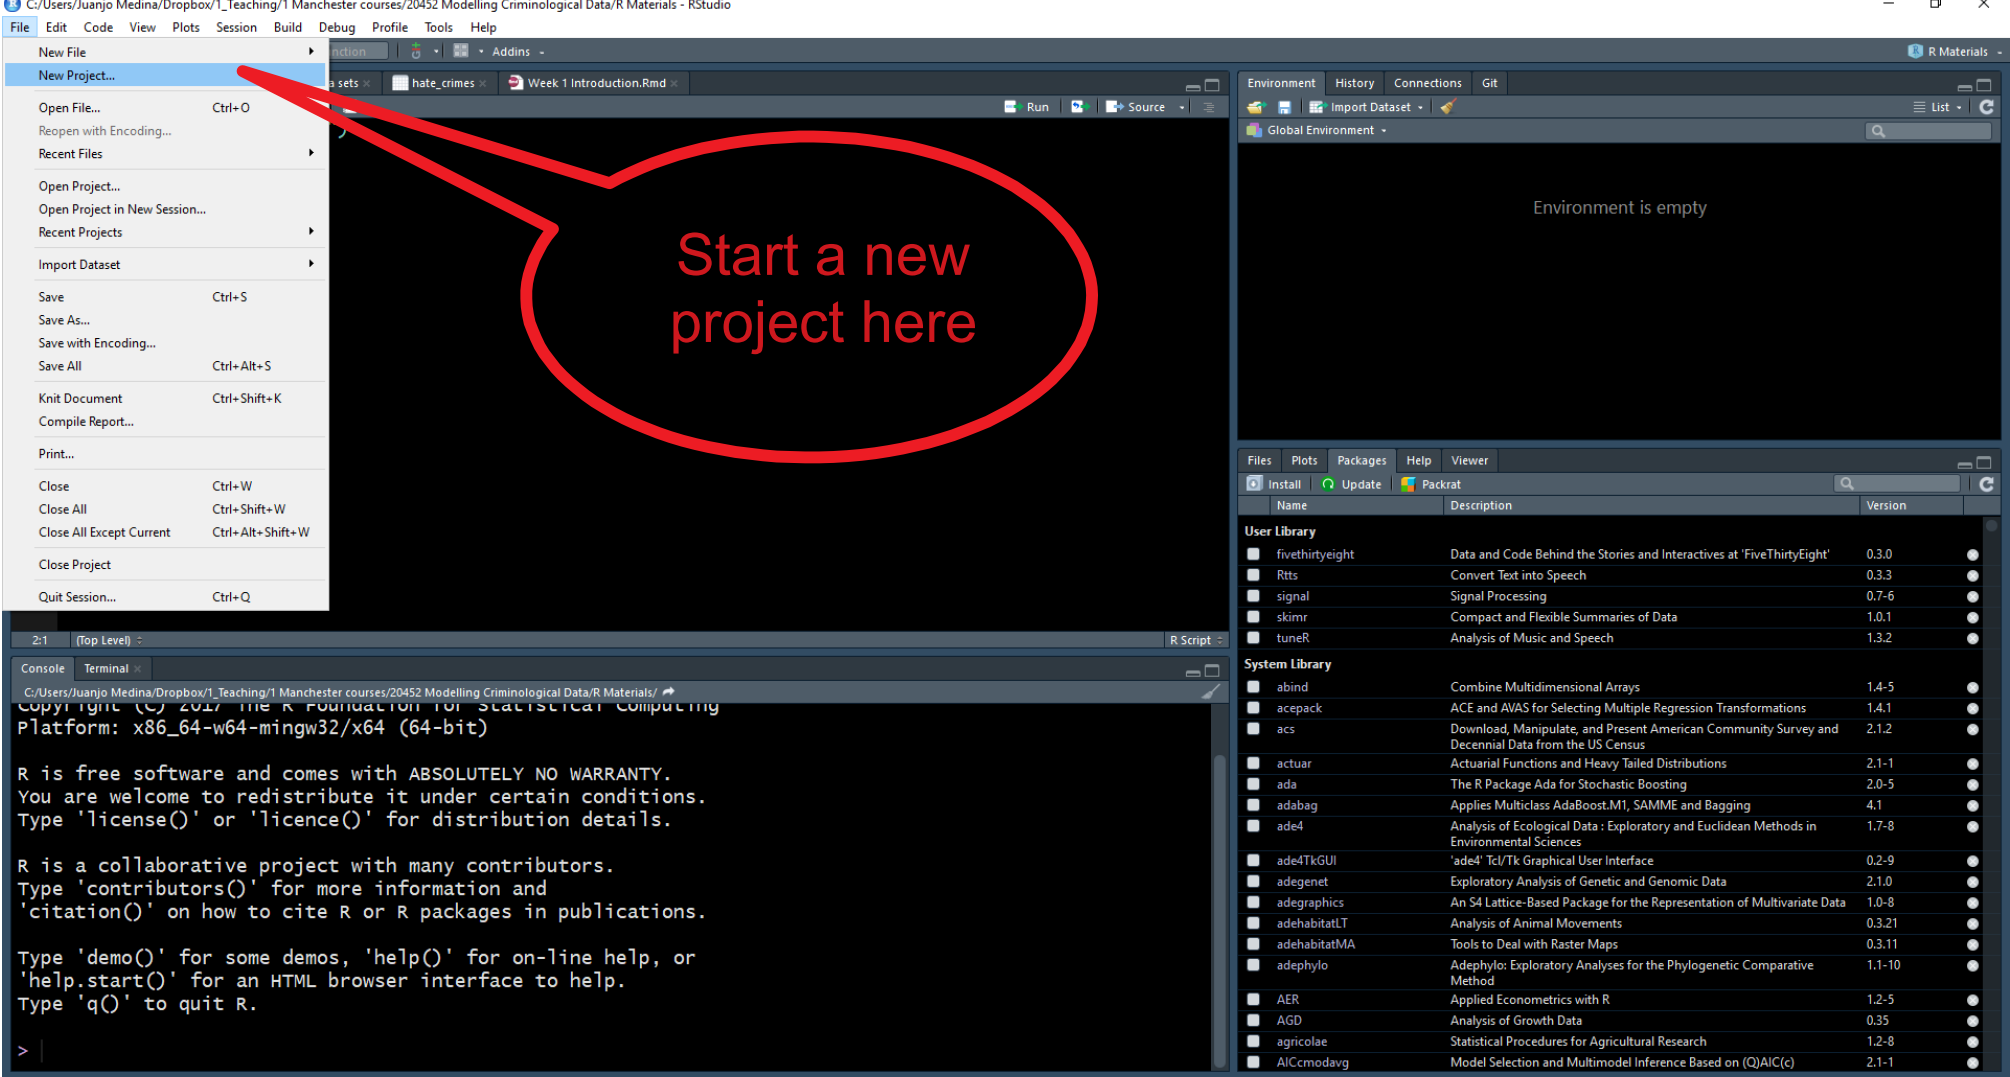
\includegraphics{imgs/newproject.png}

That will open a dialog box where you ask to specify what kind of
directory you want to create. Select new working directory in this
dialog box.

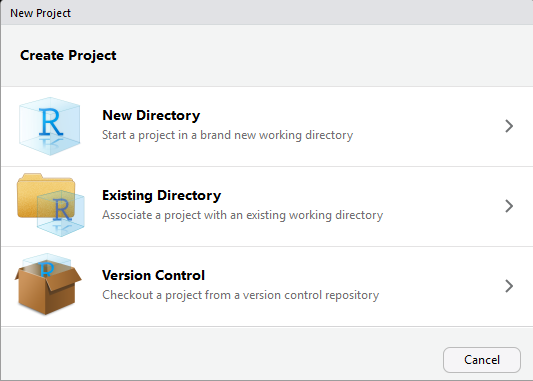
\includegraphics{imgs/newproject2.PNG}

Now you get another dialog box (at least you have an older version of R
Studio) where you have to specify what kind of project you want to
create. Select the first option \emph{New Project}.

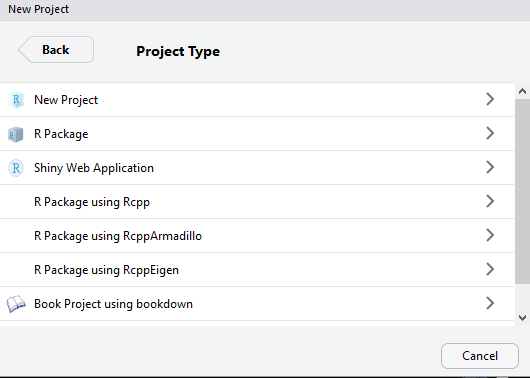
\includegraphics{imgs/newproject3.PNG}

Finally, you get to select a name for your project (in the image below I
use the code for this course unit, but you can use any sensible name you
prefer) and you will need to specify the folder in which to place this
directory. If you are using a cluster machine use the P: drive,
otherwise select what you prefer in your laptop (preferably not your
desktop in Windows machines).

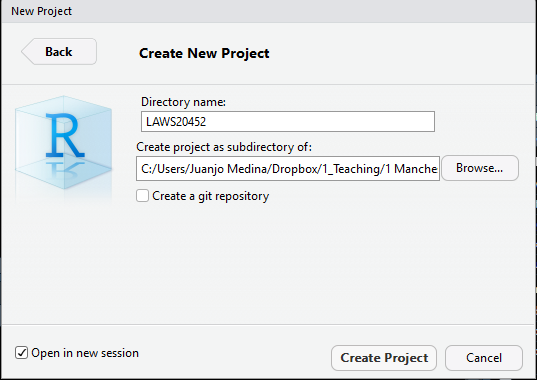
\includegraphics{imgs/newproject4.PNG}

With simple projects a single script file and a data file is all you may
have. But with more complex projects, things can rapidly become messy.
So you may want to create subdirectories within this project folder. I
typically use the following structure in my own work to put all files of
a certain type in the same subdirectory:

\begin{itemize}
\item
  \emph{Scripts and code}: Here I put all the text files with my
  analytic code, including rmarkdown files which is something we will
  introduce much later in the semester.
\item
  \emph{Source data}: Here I put the original data. I tend not to touch
  this once I have obtained the original data.
\item
  \emph{Documentation}: This is the subdirectory where I place all the
  data documentation (e.g., codebooks, questionnaires, etc.)
\item
  \emph{Modified data}: All analysis involve doing transformations and
  changing things in the original data files. You don't want to mess up
  the original data files, so what you should do is create new data
  files as soon as you start changing your source data. I go so far as
  to place them in a different subdirectory.
\item
  \emph{Literature}: Analysis is all about answering research questions.
  There is always a literature about these questions. I place the
  relevant literature for the analytic project I am conducting in this
  subdirectory.
\item
  \emph{Reports and write up}: Here is where I file all the reports and
  data visualisations that are associated with my analysis.
\end{itemize}

If you come to my office, you will see it is a very messy place. But my
computer is, in contrast, a very tidy environment. You should aim for
your computer workspace to be very organised as well. You can create
these subdirectories using Windows Explorer or the Files window in R
Studio. Why don't you have a go?

\#\#Talk to your computer

Enough background, let's write some very simple code to talk to your
computer. First open a new script within the project you just created.
Type the following instructions in the script window. After you are done
click in the top right corner where it says \emph{Run} (if you prefer
quick shortcuts, you can select the text and then press Ctrl + Enter):

\begin{Shaded}
\begin{Highlighting}[]
\KeywordTok{print}\NormalTok{(}\StringTok{"I hate computers"}\NormalTok{)}
\end{Highlighting}
\end{Shaded}

\begin{verbatim}
## [1] "I hate computers"
\end{verbatim}

Congratulations!!! You just run your first line of R code! Though that
was a really mean thing to say to your machine!

In these handouts (written in html format) you will see grayed boxes
with bit of code on it. You can cut and paste this code into your script
window and run the code from it to reproduce our results. As we go along
we will be covering new bits of code. You should start thinking about
creating a file with some of the most useful bits of code we cover so
that when you do your work you can just cut and paste from this file
rather than having to come back to these handouts.

Sometimes in these documents you will see on them the results of running
the code, what you see printed in your console or in your plot viewer.
The results will appear enclosed in a box as above.

The R languages uses \textbf{functions} to tell the computer what to do.
In the R \emph{language} functions are the \emph{verbs}. You can think
of functions as predefined commands that somebody has already programmed
into R and tell R what to do. Here you learnt your first R function:
\emph{print}. All this function does is to ask R to print whatever it is
you want in the main console (see the window in the bottom left corner).

In R, you can pass a number of \textbf{arguments} to any function. These
arguments control what the function will do in each case. The arguments
appear between brackets. Here we passed the text ``I hate computers'' as
an argument. Once you execute the program, by clicking on \emph{Run},
the R engine sends this to the CPU of your machine in the form of binary
code and this produces a result. In this case we see that result printed
in the main console.

Every R function admits different kind of arguments. Learning R involves
not only learning different functions but also learning what are the
valid arguments you can pass to each function.

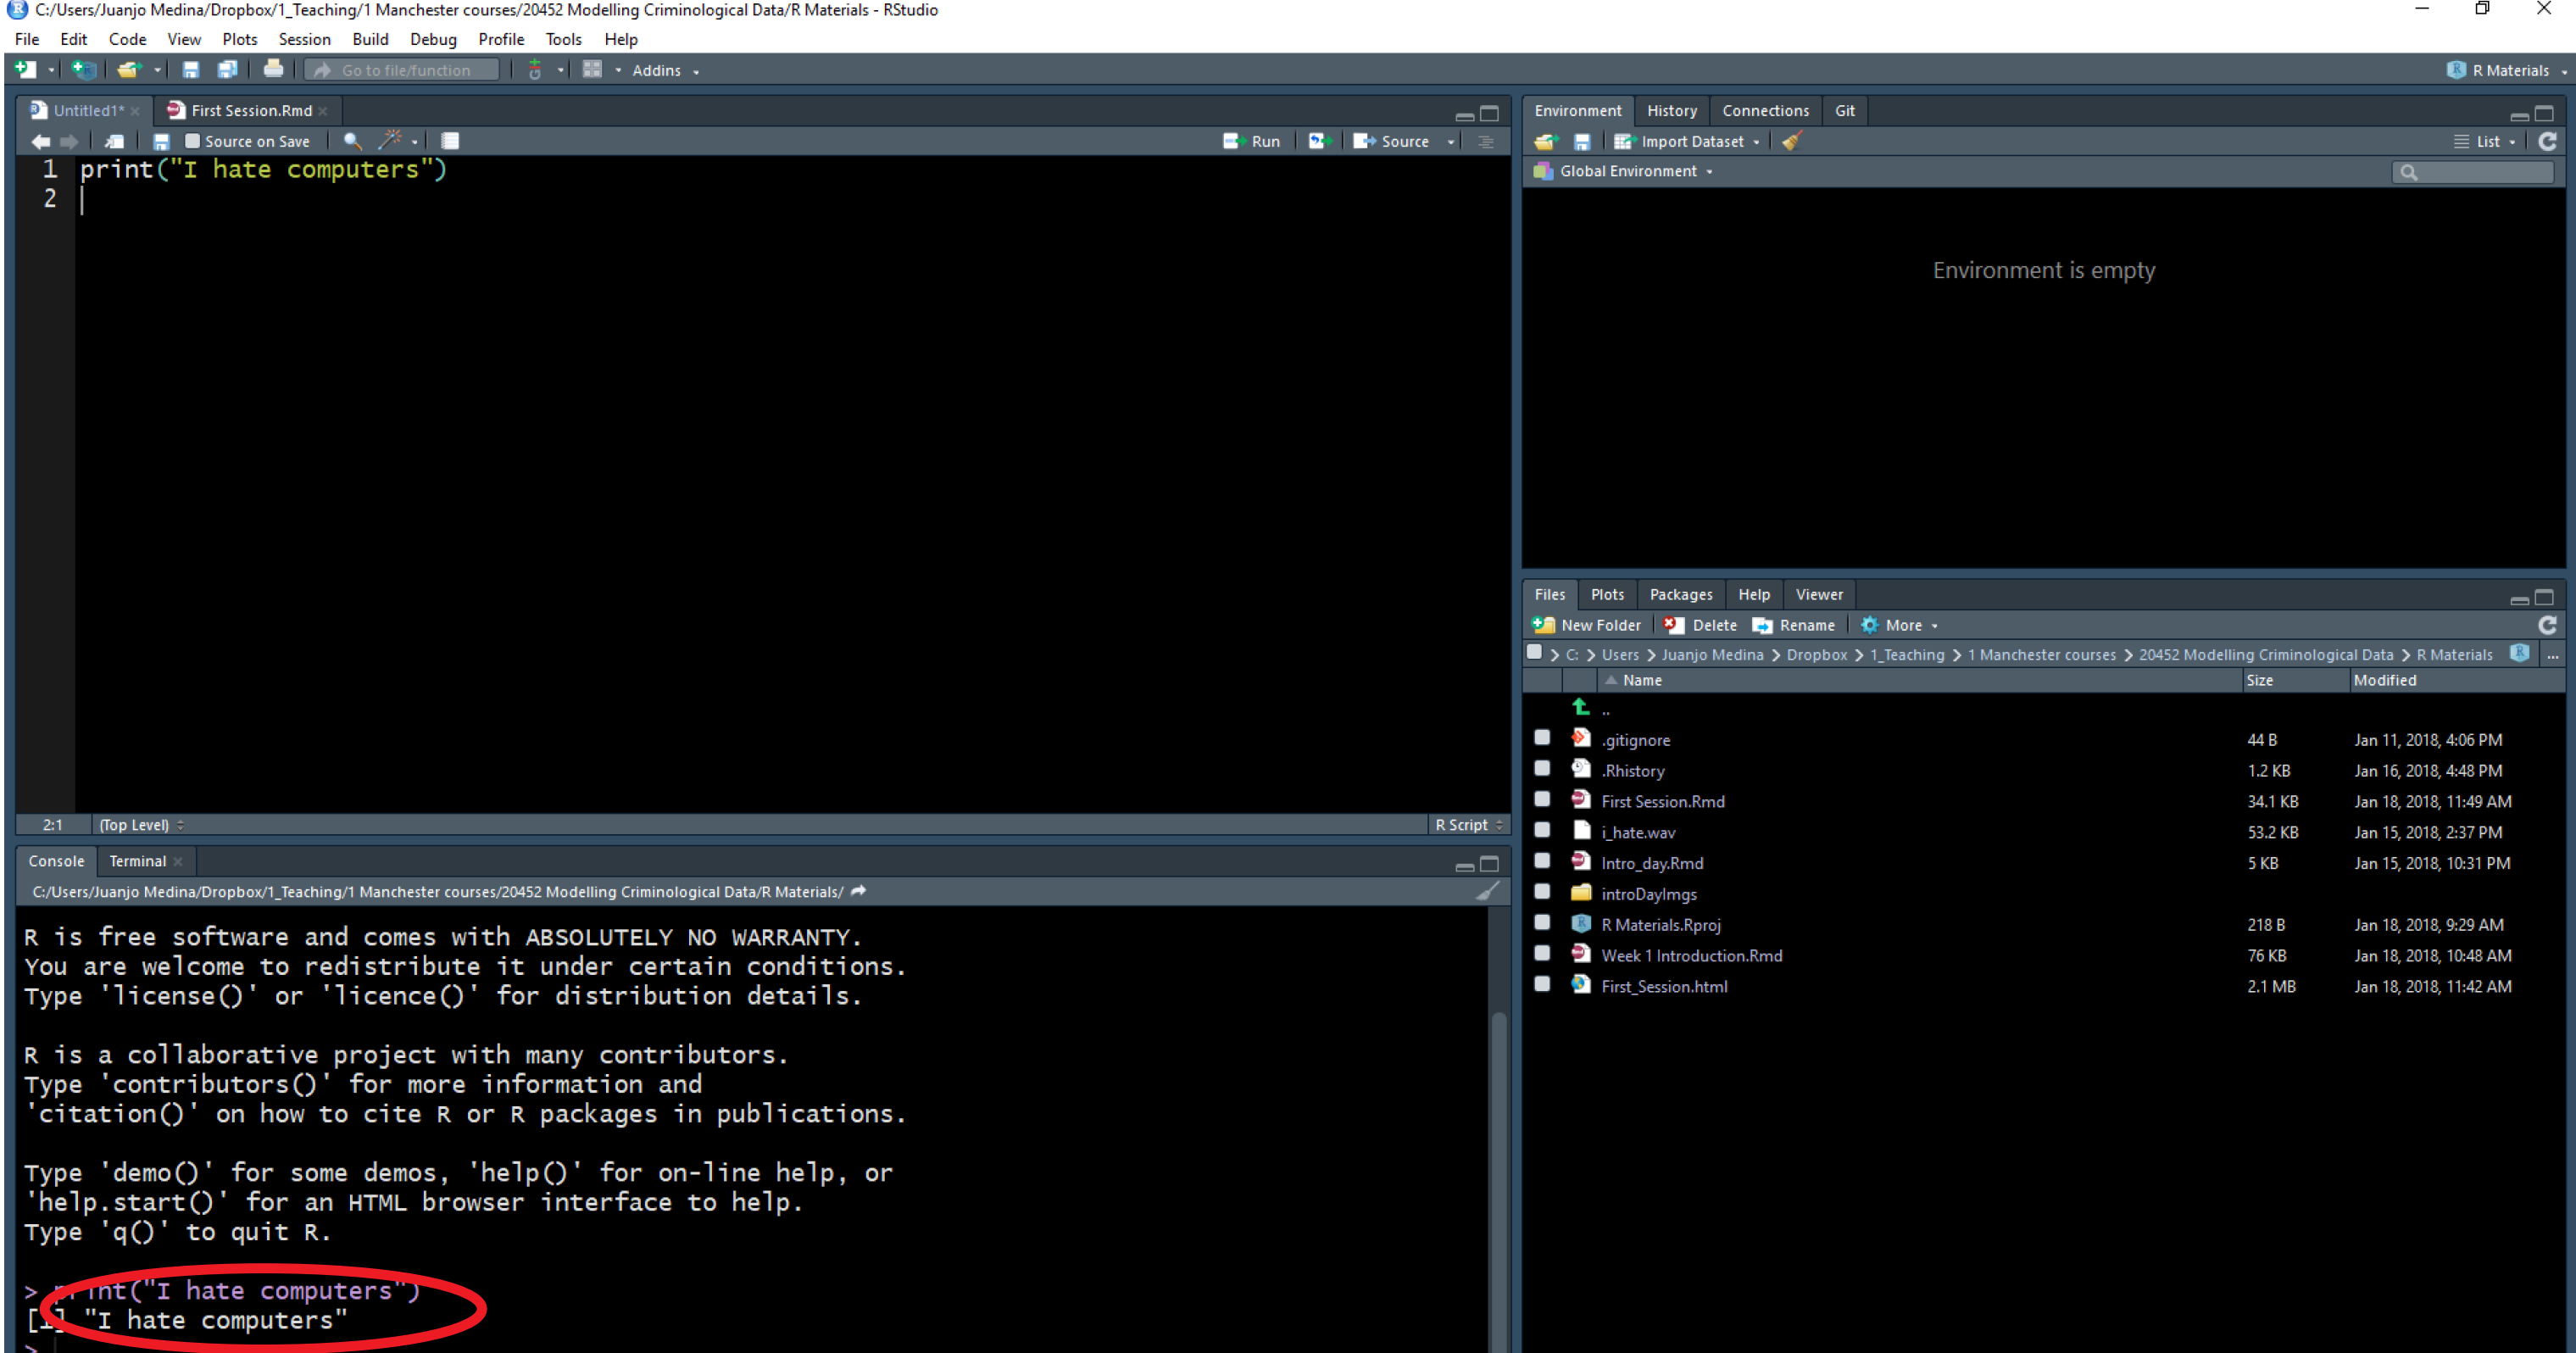
\includegraphics{imgs/consoleresults.png} As indicated above, the window
in the bottom left corner is the main \textbf{console}.You will see that
the words ``I hate computers'' appear printed there. If rather than
using R Studio you were working directly from R, that's all you would
get: the main console where you can write code interactively (rather
than all the different windows you see in R Studio). You can write your
code directly in the main console and execute it line by line in an
interactive fashion. However, we will be running code from scripts, so
that you get used to the idea of properly documenting all the steps you
take,

\#\#More on packages

Before we described packages as elements that add the functionality of
R. What most packages do is they introduce new functions that allow you
to ask R to do new different things.

Anybody can write a package, so consequently R packages vary on quality
and complexity. You can find packages in different places, as well, from
official repositories (which means they have passed a minimum of quality
control), something called Git Hub (a webpage where software developers
post work in progress), to personal webpages (danger danger!). In early
2017 we passed the 10,000 mark just in the main official repository, so
the number of things that can be done with R grows exponentially every
day as people keep adding new packages.

When you install R you only install a set of basic packages, not the
full 10,000 plus. So if you want to use any of these added packages that
are not part of the basic installation you need to first install them.
You can see what packages are availabe in your local install by looking
at the \emph{packages} tab in the bottom right corner panel. Click there
and check. We are going to install a package that is not there so that
you see how the installation is done.

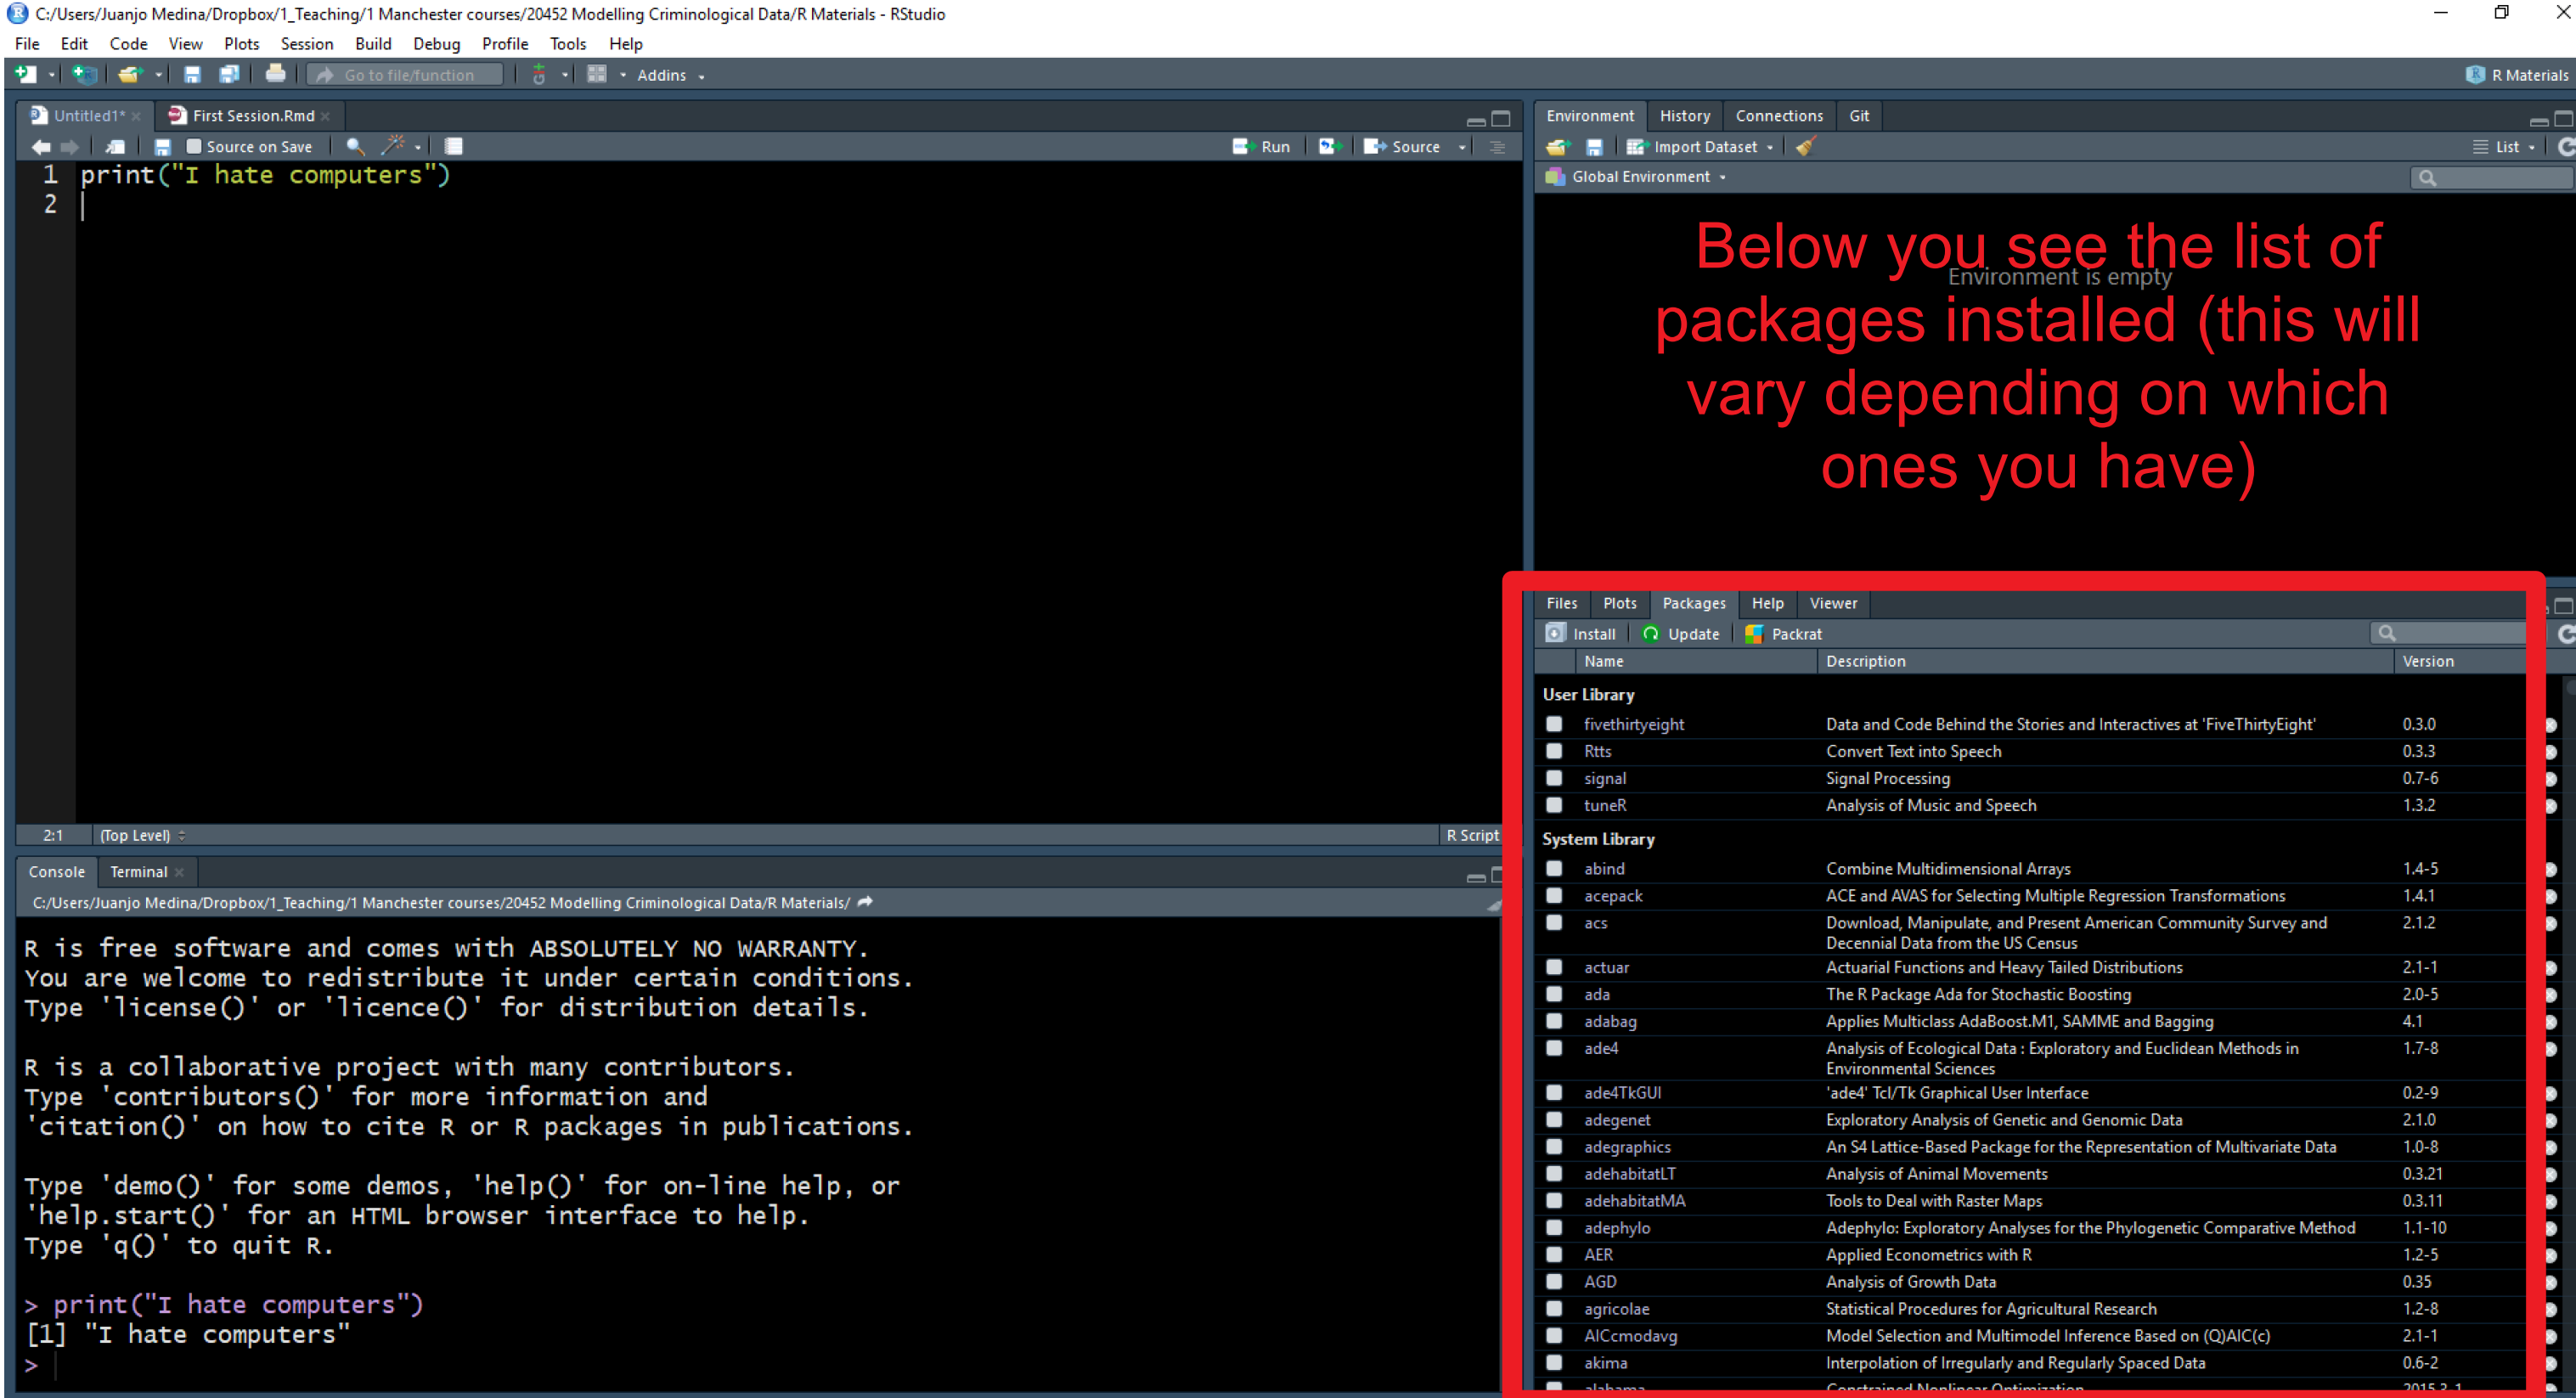
\includegraphics{imgs/packages.png}

If you just installed R in your laptop you will see a shortish list of
packages that constitute the basic installation of R. If you are using
one of the machines in the computer cluster this list is a bit longer,
because we asked IT to install some of the most commonly used packages.
But knowing how to install packages is pretty essential, since you will
want to do it very often.

We are going to install a package called ``cowsay'' to demonstrate the
process. In the Packages panel there is an \emph{Install} menu that
would open a dialog box and allows you to install packages. Instead we
are going to use code to do this. Just cut and paste the code below into
your script and then run it:

\begin{Shaded}
\begin{Highlighting}[]
\KeywordTok{install.packages}\NormalTok{(}\StringTok{"cowsay"}\NormalTok{)}
\end{Highlighting}
\end{Shaded}

Here we are introducing a new function ``install.packages'' and what we
have passed as an argument is the name of the package that we want to
install. This is how we install a package \emph{that is available in the
official CRAN repository}. If we wanted to install a package from
somewhere else we would have to adapt the code. Later this semester you
will see how we install packages from Git Hub.

This line of code (as it is currently written) will install this package
in a personal library that will be located in your P: drive if you are
using a cluster machine. If you are using a Windows machine this will
place this package within a personal library in your Documents folder.
Once you install a package is in the machine/location where you install
it until you physically delete it. The code we have used by default
connects to a cloud repository called
\href{https://cran.r-project.org/}{CRAN} that has a collection of R
packages that meet a minimum set of quality criteria. CRAN is the
official repository of all things R. It's a fairly safe place to get
packages from. But beware, judging whether a package is good or not
requires your input. We will come back to this several times during the
semester to help you make wise choices regarding packages. Given that
you are connecting to an online repository you will need an internet
connection every time you want to install a package.

How do you find out what a package does? You look at the relevant
documentation. In the Packages window scroll down until you find the new
package we installed listed. Here you will see the name of the package
(cowsay), a brief description of what the program is about, and the
version you have installed (an indication that a package is a good
package is that it has gone through several versions, that means that
someone is making sure the package gets regular updates and
improvements). The version I have for cowsay is 0.7.0. Yours may be
older or newer. It doesn't matter much at this point.

Click in the name \emph{cowsay}. You will see that R Studio has now
brought you to the Help tab. Here is where you find the help files for
this package, including all the available documentation.

Every beginner in R will find these help files a bit confusing. But
after a while, their format and structure will begin to make sense to
you. Click where it says \emph{User guides, package vignettes, and other
documentation}. Documentation in R has become much better since people
started to write \textbf{vignettes} for their packages. They are little
tutorials that explain with examples what each package does. Click in
the \emph{cowsay::cowsay\_tutorial} that you see listed here (the html
link). What you will find there is an html file that gives you a
detailed tutorial on this package. You don't need to read it now, but
remember that this is one way to find help when using R. You will learn
to love vignettes.

Let's try to use some of the functions of this package. We will use the
``say'' function:

\begin{Shaded}
\begin{Highlighting}[]
\KeywordTok{say}\NormalTok{(}\StringTok{"I hate computers"}\NormalTok{)}
\end{Highlighting}
\end{Shaded}

You will get an error message telling you that this function could not
be found. What happened? Installing a package is only the first step.
The next step, when you want to use it in a given session, is to
\textbf{load} it.

Think of it as a pair of shoes. You buy it once, but you have to take
them from your closet and put them on when you want to use them. Same
with packages, you only install once, but need to load it from your
library every time you want to use it -within a given session (once
loaded it will remain loaded until you finish your session).

To see what packages you currently have \textbf{loaded} in your session,
you use the \texttt{search()} function (you do not need to pass it any
arguments in this case).

\begin{Shaded}
\begin{Highlighting}[]
\KeywordTok{search}\NormalTok{()}
\end{Highlighting}
\end{Shaded}

\begin{verbatim}
## [1] ".GlobalEnv"        "package:stats"     "package:graphics" 
## [4] "package:grDevices" "package:utils"     "package:datasets" 
## [7] "package:methods"   "Autoloads"         "package:base"
\end{verbatim}

If you run this code, you will see that \texttt{cowsay} is not in the
list of loaded packages. To load a package we use the \textbf{library}
function. So if we want to load the new package we installed in our
machine we would need to use the following code:

\begin{Shaded}
\begin{Highlighting}[]
\KeywordTok{library}\NormalTok{(}\StringTok{"cowsay"}\NormalTok{)}
\end{Highlighting}
\end{Shaded}

Run the \texttt{search} function again. You will see now this package is
listed. So now we can try using the function ``say'' again.

\begin{Shaded}
\begin{Highlighting}[]
\KeywordTok{say}\NormalTok{(}\StringTok{"I hate computers"}\NormalTok{)}
\end{Highlighting}
\end{Shaded}

\begin{verbatim}
## Colors cannot be applied in this environment :( Try using a terminal or RStudio.
\end{verbatim}

\begin{verbatim}
## 
##  -------------- 
## I hate computers 
##  --------------
##     \
##       \
##         \
##             |\___/|
##           ==) ^Y^ (==
##             \  ^  /
##              )=*=(
##             /     \
##             |     |
##            /| | | |\
##            \| | |_|/\
##       jgs  //_// ___/
##                \_)
## 
\end{verbatim}

You get a random animal in the console repeating the text we passed as
an argument. If we like a different animal we could pass an argument to
select it. So, say, we want to have cow rather than a random animal,
then we would pass the following arguments to our function.

\begin{Shaded}
\begin{Highlighting}[]
\KeywordTok{say}\NormalTok{(}\StringTok{"I hate computers"}\NormalTok{, }\StringTok{"cow"}\NormalTok{)}
\end{Highlighting}
\end{Shaded}

\begin{verbatim}
## Colors cannot be applied in this environment :( Try using a terminal or RStudio.
\end{verbatim}

\begin{verbatim}
## 
##  ----- 
## I hate computers 
##  ------ 
##     \   ^__^ 
##      \  (oo)\ ________ 
##         (__)\         )\ /\ 
##              ||------w|
##              ||      ||
\end{verbatim}

Remember, you only have to install a package that is not already
installed once. But if you want to use it in a given session you will
have to load it within that session using the \texttt{library} function.
Once you load it within a session the package will remain loaded until
you terminate your session (for example, by closing R Studio).

\#\#Using objects

We have seen how the first argument that the ``say'' function takes is
the text that we want to convert into speech for our given animal. We
could write the text directly into the function, but now we are going to
do something different. We are going to create an object to store the
text.

An \textbf{object}? What do I mean? In the same way that everything you
do in R you do with functions (your verbs), everything that exist in R
is an object. You can think of objects as boxes where you put stuff. In
this case we are going to create an object called \emph{my\_text} and
inside this object we are going to store the text ``I hate computers''.
How do you do this? We will use the code below:

\begin{Shaded}
\begin{Highlighting}[]
\NormalTok{my_text <-}\StringTok{ "I hate computers."}
\end{Highlighting}
\end{Shaded}

This bit of code is simply telling R we are creating a new object with
the assigned name (``my\_text''). We are creating a box with such name
and inside this box we are placing a bit of text (``I hate computers'').
The arrow you see is the \textbf{assignment operator}. This is an
important part of the R language that tells R what we are including
inside the object in question.

Run the code. Look now at the \emph{Environment} window in the right top
corner. We see that this object is now listed there. You can think of
the Environment as a warehouse where you put stuff in, your different
objects. Is there a limit to this environment? Yes, your RAM. R works on
your RAM, so you need to be aware that if you use very large objects you
will need loads of RAM. But that won't be a problem you will encounter
in this course unit.

Once we put things into these boxes or objects we can use them as
arguments in our functions. See the example below:

\begin{Shaded}
\begin{Highlighting}[]
\KeywordTok{say}\NormalTok{(my_text, }\StringTok{"cow"}\NormalTok{)}
\end{Highlighting}
\end{Shaded}

\begin{verbatim}
## Colors cannot be applied in this environment :( Try using a terminal or RStudio.
\end{verbatim}

\begin{verbatim}
## 
##  ----- 
## I hate computers. 
##  ------ 
##     \   ^__^ 
##      \  (oo)\ ________ 
##         (__)\         )\ /\ 
##              ||------w|
##              ||      ||
\end{verbatim}

\#\#More on objects

Isn't this a course on data analysis? Yes, of course, but before we get
there, you need to get used to the basics of R and R Studio, which is
what we will be doing in these early sessions. Let's go through some of
these basics a bit more slowly to ensure you get them and then we will
bring some data you can look at.

In Excel you are used to see your data in a spreadsheet format. If you
did the prep for this session, you should have reviewed some of the
materials we covered in \emph{Making Sense of Criminological Data} last
semester. You should be familiar with the notion of a data set, levels
of measurement, and tidy data. If you have not. This is your chance to
do it in
\href{https://rawgit.com/maczokni/MSCD/master/book/bookdown-demo-master/bookdown-demo-master/docs/week1.html\#data-variables-and-observations}{this
link}.

R is considerably more flexible than Excel. Most of the work we do here
will use data sets or \textbf{dataframes} as they are called in R. But
as you have seen earlier you can have \emph{objects} other than data
frames in R. These objects can relate to external files or simple
textual information (``I hate computers''). This flexibility is a big
asset because among other things it allow us to break down data frames
or the results from doing analysis on them to its constitutive parts
(this will become clearer as we go along).

Technically R is an \emph{Object Oriented language}. Object-oriented
programming (OOP) is a programming language model organized around
objects rather than ``actions'' and data rather than logic.

As we have seen earlier, to create an object you have to give it a name,
and then use the assignment operator (the \texttt{\textless{}-} symbol)
to assign it some value.

For example, if we want to create an object that we name ``x'', and we
want it to represent the value of 5, we write:

\begin{Shaded}
\begin{Highlighting}[]
\NormalTok{x <-}\StringTok{ }\DecValTok{5}
\end{Highlighting}
\end{Shaded}

We are simply telling R to create a \textbf{numeric object}, called
\texttt{x}, with one element (5) or of length 1. It is numeric because
we are putting a number inside this object. The length is 1 because it
only has one element on it, the number 5.

You can see the content of the object \texttt{x} in the main console
either by using the print function we used earlier or by auto-printing,
that is, just typing the name of the object and running that as code:

\begin{Shaded}
\begin{Highlighting}[]
\NormalTok{x}
\end{Highlighting}
\end{Shaded}

\begin{verbatim}
## [1] 5
\end{verbatim}

When writing expressions in R is very important you understand that
\textbf{R is case sensitive}. This could drive you nuts if you are not
careful. More often than not if you write an expression asking R to do
something and R returns an error message, chances are that you have used
lower case when upper case was needed (or vice-versa). So always check
for the right spelling. For example, see what happens if I use a capital
`X':

\begin{Shaded}
\begin{Highlighting}[]
\NormalTok{X}
\end{Highlighting}
\end{Shaded}

\begin{verbatim}
## Error in eval(expr, envir, enclos): object 'X' not found
\end{verbatim}

You will get the following message:
\texttt{"Error\ in\ eval(expr,\ envir,\ enclos):\ object\ \textquotesingle{}X\textquotesingle{}\ not\ found"}.
R is telling us that \texttt{X} does not exist. There isn't an object
\texttt{X} (upper case), but there is an object \texttt{x} (lower case).
Error messages in R are pretty good at telling you exactly what went
wrong.

Remember computers are very literal. They are like dogs. You can tell a
dog ``sit'' and if it has been trained it will sit. But if you tell a
dog ``would you be so kind as to relax a bit and lay down in the
sofa?'', it won't have a clue what you are saying and will stare at you
like you have gone mad. Error messages are computers ways of telling us
``I really want to help you but I don't really understand what you
mean'' (never take them personal, computers don't hate you).

When you get an error message or implausible results, you want to look
back at your code to figure out what is the problem. This process is
called \textbf{debugging}. There are some proper systematic ways to
write code that facilitate debugging, but we won't get into that here. R
is very good with automatic error handling at the levels we'll be using
it at. Very often the solution will simply involve correcting the
spelling.

A handy tip is to cut and paste the error message into Google and find a
solution. If anybody had given me a penny for every time I had to do
that myself, I would be Bill Gates by now. People make mistakes all the
time. It's how we learn. Don't get frustrated, don't get stuck. Instead
look for a solution. These days we have Google. We didn't back in the
day. Now you have the answer to your frustration within quick reach. Use
it to your advantage.

\#\#Vectors

Now that you are a bit more familiar with the idea of an object, we can
start talking about a particular type of objects, specifically we are
going to discuss \textbf{vectors}.

What is a vector? A vector is simply a set of elements \emph{of the same
class} (typically these classes are: character, numeric, integer, or
logical -as in True/False). Vectors are the basic data structure in R.

Typically you will use the \texttt{c()} function (c stands for
concatenate) to create vectors. The code below exemplifies how to create
vectors of different classes (numeric, logical, etc.). Notice how the
listed elements (to simplify there are two elements in each vector
below) are separated by commas:

\begin{Shaded}
\begin{Highlighting}[]
\NormalTok{my_1st_vector <-}\StringTok{ }\KeywordTok{c}\NormalTok{(}\FloatTok{0.5}\NormalTok{, }\FloatTok{0.6}\NormalTok{) }\CommentTok{#creates a numeric vector with two elements}
\NormalTok{my_2nd_vector <-}\StringTok{ }\KeywordTok{c}\NormalTok{(1L, 2L) }\CommentTok{#creates an integer vector}
\NormalTok{my_3rd_vector <-}\StringTok{ }\KeywordTok{c}\NormalTok{(}\OtherTok{TRUE}\NormalTok{, }\OtherTok{FALSE}\NormalTok{) }\CommentTok{#creates a logical vector}
\NormalTok{my_4th_vector <-}\StringTok{ }\KeywordTok{c}\NormalTok{(T, F) }\CommentTok{#creates a logical vector using abbreviations of True and False, but you should avoid this formulation an instead use the full word.}
\NormalTok{my_5th_vector <-}\StringTok{ }\KeywordTok{c}\NormalTok{(}\StringTok{"a"}\NormalTok{, }\StringTok{"b"}\NormalTok{, }\StringTok{"c"}\NormalTok{) }\CommentTok{#creates a character vector}
\NormalTok{my_6th_vector <-}\StringTok{ }\KeywordTok{c}\NormalTok{(}\DecValTok{1}\OperatorTok{+}\NormalTok{0i, }\DecValTok{2}\OperatorTok{+}\NormalTok{4i) }\CommentTok{#creates a complex vector (we won't really use this class)}
\end{Highlighting}
\end{Shaded}

Cut and paste this code into your script and run it. You will see how
all these vectors are added to your global environment and stored there.

The beauty of an object oriented statistical language like R is that one
you have these objects you can use them as \textbf{inputs} in functions,
use them in operations, or to create other objects. This makes R very
flexible. See some examples below:

\begin{Shaded}
\begin{Highlighting}[]
\KeywordTok{class}\NormalTok{(my_1st_vector) }\CommentTok{#a function to figure out the class of the vector}
\end{Highlighting}
\end{Shaded}

\begin{verbatim}
## [1] "numeric"
\end{verbatim}

\begin{Shaded}
\begin{Highlighting}[]
\KeywordTok{length}\NormalTok{(my_1st_vector) }\CommentTok{#a function to figure out the length of the vector}
\end{Highlighting}
\end{Shaded}

\begin{verbatim}
## [1] 2
\end{verbatim}

\begin{Shaded}
\begin{Highlighting}[]
\NormalTok{my_1st_vector }\OperatorTok{+}\StringTok{ }\DecValTok{2} \CommentTok{#Add a constant to each element of the vector}
\end{Highlighting}
\end{Shaded}

\begin{verbatim}
## [1] 2.5 2.6
\end{verbatim}

\begin{Shaded}
\begin{Highlighting}[]
\NormalTok{my_7th_vector <-}\StringTok{ }\NormalTok{my_1st_vector }\OperatorTok{+}\StringTok{ }\DecValTok{1} \CommentTok{#Create a new vector that contains the elements of my1stvector plus a constant of 1}
\NormalTok{my_1st_vector }\OperatorTok{+}\StringTok{ }\NormalTok{my_7th_vector }\CommentTok{#Adds the two vectors and auto-print the results (note how the sum was done)}
\end{Highlighting}
\end{Shaded}

\begin{verbatim}
## [1] 2.0 2.2
\end{verbatim}

As indicated earlier, when you create objects you will place them in
your working memory or workspace. Each R session will be associated to a
workspace (called ``global environment'' in R Studio). In R Studio you
can visualise the objects you have created during a session in the
\textbf{Global Environment} screen. But if you want to produce a list of
what's there you can use the \texttt{ls()} function (the results you get
my differ from the ones below depending on what you actually have in
your global environment).

\begin{Shaded}
\begin{Highlighting}[]
\KeywordTok{ls}\NormalTok{() }\CommentTok{#list all objects in your global environment}
\end{Highlighting}
\end{Shaded}

\begin{verbatim}
## [1] "my_1st_vector" "my_2nd_vector" "my_3rd_vector" "my_4th_vector"
## [5] "my_5th_vector" "my_6th_vector" "my_7th_vector" "my_text"      
## [9] "x"
\end{verbatim}

If you want to delete a particular object you can do so using the
\texttt{rm()} function.

\begin{Shaded}
\begin{Highlighting}[]
\KeywordTok{rm}\NormalTok{(x) }\CommentTok{#remove x from your global environment}
\end{Highlighting}
\end{Shaded}

It is also possibly to remove all objects at once:

\begin{Shaded}
\begin{Highlighting}[]
\KeywordTok{rm}\NormalTok{(}\DataTypeTok{list =} \KeywordTok{ls}\NormalTok{()) }\CommentTok{#remove all objects from your global environment}
\end{Highlighting}
\end{Shaded}

If you mix in a vector elements that are of a different class (for
example numerical and logical), R will \textbf{coerce} to the minimum
common denominator, so that every element in the vector is of the same
class. So, for example, if you input a number and a character, it will
coerce the vector to be a character vector -see the example below and
notice the use of the \texttt{class()} function to identify the class of
an object.

\begin{Shaded}
\begin{Highlighting}[]
\NormalTok{my_8th_vector <-}\StringTok{ }\KeywordTok{c}\NormalTok{(}\FloatTok{0.5}\NormalTok{, }\StringTok{"a"}\NormalTok{)}
\KeywordTok{class}\NormalTok{(my_8th_vector) }\CommentTok{#The class() function will tell us the class of the vector}
\end{Highlighting}
\end{Shaded}

\begin{verbatim}
## [1] "character"
\end{verbatim}

\#\#On comments

In the bits of code above you will have noticed parts that were grayed
out. See for example in the last example provided. You can see that
after the hash-tag all the text is being grayed out. What is this?
What's going on?

These are \textbf{comments}. Comments are simply annotations that R will
know is not code (and therefore doesn't attempt to understand and
execute). We use the hash-tag symbol to specify to R that what comes
after is not programming code, but simply bits of notes that we write to
remind ourselves what the code is actually doing. Including these
comments will help you to understand your code when you come back to it.

To create a comment you use the hash-tag/ number sign \texttt{\#}
followed by some text. Whenever the R engine sees the number sign it
knows that what follows is not code to be executed. You can use this
sign to include \emph{annotations} when you are coding. These
annotations are a helpful reminder to yourself (and others reading your
code) of \textbf{what} the code is doing and (even more important)
\textbf{why} you are doing it.

It is good practice to often use annotations. You can use these
annotations in your code to explain your reasoning and to create
``scannable'' headings in your code. That way after you save your script
you will be able to share it with others or return to it at a later
point and understand what you were doing when you first created it -see
\href{http://www.screenr.com/1VN8}{here for further details on
annotations and in how to save a script when working with the basic R
interface}.

Just keep in mind: + You need one \texttt{\#} per line, and anything
after that is a comment that is not executed by R.

\begin{itemize}
\tightlist
\item
  You can use spaces after (its not like a hash-tag on twitter).
\end{itemize}

\#\#Factors

An important thing to understand in R is that categorical (ordered, also
called ordinal, or unordered, also called nominal) data are typically
encoded as \textbf{factors}, which are just a special type of vector. A
factor is simply an integer vector that can contain \emph{only
predefined values} (this bit is very important), and is used to store
categorical data. Factors are treated specially by many data analytic
and visualisation functions. This makes sense because they are
essentially different from quantitative variables.

Although you can use numbers to represent categories, \emph{using
factors with labels is better than using integers to represent
categories} because factors are self-describing (having a variable that
has values ``Male'' and ``Female'' is better than a variable that has
values ``1'' and ``2'' to represent male and female). When R reads data
in other formats (e.g., comma separated), by default it will
automatically convert all character variables into factors. If you
rather keep these variables as simple character vectors you need to
explicitly ask R to do so. We will come back to this next week with some
examples.

Factors can also be created with the \texttt{factor()} function
concatenating a series of \emph{character} elements. You will notice
that is printed differently from a simply character vector and that it
tells us the levels of the factor (look at the second printed line).

\begin{Shaded}
\begin{Highlighting}[]
\NormalTok{the_smiths <-}\StringTok{ }\KeywordTok{factor}\NormalTok{(}\KeywordTok{c}\NormalTok{(}\StringTok{"Morrisey"}\NormalTok{, }\StringTok{"Marr"}\NormalTok{, }\StringTok{"Rourke"}\NormalTok{, }\StringTok{"Joyce"}\NormalTok{)) }\CommentTok{#create a new factor}
\NormalTok{the_smiths }\CommentTok{#auto-print the factor}
\end{Highlighting}
\end{Shaded}

\begin{verbatim}
## [1] Morrisey Marr     Rourke   Joyce   
## Levels: Joyce Marr Morrisey Rourke
\end{verbatim}

\begin{Shaded}
\begin{Highlighting}[]
\CommentTok{#Alternatively for similar result using the as.factor() function}
\NormalTok{the_smiths_bis <-}\StringTok{ }\KeywordTok{c}\NormalTok{(}\StringTok{"Morrisey"}\NormalTok{, }\StringTok{"Marr"}\NormalTok{, }\StringTok{"Rourke"}\NormalTok{, }\StringTok{"Joyce"}\NormalTok{) }\CommentTok{#create a character vector}
\NormalTok{the_smiths_f <-}\StringTok{ }\KeywordTok{as.factor}\NormalTok{(the_smiths_bis) }\CommentTok{#create a factor using a character vector}
\NormalTok{the_smiths_f }\CommentTok{#auto-print factor}
\end{Highlighting}
\end{Shaded}

\begin{verbatim}
## [1] Morrisey Marr     Rourke   Joyce   
## Levels: Joyce Marr Morrisey Rourke
\end{verbatim}

Factors in R can be seen as vectors with a bit more information added.
This extra information consists of a record of the distinct values in
that vector, called \textbf{levels}. If you want to know the levels in a
given factor you can use the \texttt{levels()} function:

\begin{Shaded}
\begin{Highlighting}[]
\KeywordTok{levels}\NormalTok{(the_smiths)}
\end{Highlighting}
\end{Shaded}

\begin{verbatim}
## [1] "Joyce"    "Marr"     "Morrisey" "Rourke"
\end{verbatim}

Notice that the levels appear printed by alphabetical order. There will
be situations when this is not the most convenient order. Later on we
will discuss in these tutorials how to reorder your factor levels when
you need to.

\#\#Naming conventions for objects in R

You may have noticed the various names I have used to designate objects
(\texttt{my\_1st\_vector}, \texttt{the\_smiths}, etc.). You can use
almost any names you want for your objects. Objects in R can have names
of any length consisting of letters, numbers, underscores ("\_``) or the
period (''.") and should begin with a letter. In addition, when naming
objects you need to remember:

\begin{itemize}
\item
  \emph{Some names are forbidden}. These include words such as FALSE and
  TRUE, logical operators, and programming words like Inf, for, else,
  break, function, and words for special entities like NA and NaN.
\item
  \emph{You want to use names that do not correspond to a specific
  function.} We have seen, for example, that there is a function called
  \texttt{print()}, you don't want to call an object ``print'' to avoid
  conflicts. To avoid this use nouns instead of verbs for naming your
  variables and data.
\item
  \emph{You don't want them to be too long} (or you will regret it every
  time you need to use that object in your analysis: your fingers will
  bleed from typing).
\item
  \emph{You want to make them as intuitive to interpret as possible.}
\item
  \emph{You want to follow consistent naming conventions.}
  \href{http://journal.r-project.org/archive/2012-2/RJournal_2012-2_Baaaath.pdf}{R
  users are terrible about this}. But we could make it better if we all
  aim to follow similar conventions. In these handouts you will see I
  follow the \texttt{underscore\_separated} convention -see
  \href{http://robinlovelace.net/r/2014/07/15/naming-conventions-r.html}{here}
  for details.
\end{itemize}

It is also important to remember that R will always treat numbers as
numbers. This sounds straightforward, but actually it is important to
note. We can name our variables almost anything. EXCEPT they cannot be
numbers. Numbers are \textbf{protected} by R. 1 will always mean 1.

If you want, give it a try. Try to create a variable called 12 and
assign it the value ``twelve''. As we did last week, we can assign
something a meaning by using the ``\textless{}-'' characters.

\begin{Shaded}
\begin{Highlighting}[]
\DecValTok{12}\NormalTok{ <-}\StringTok{ "twelve"}
\end{Highlighting}
\end{Shaded}

\begin{verbatim}
## Error in 12 <- "twelve": invalid (do_set) left-hand side to assignment
\end{verbatim}

You get an error!

\#\#Dataframes

Ok, so now that you understand some of the basic types of objects you
can use in R, let's start taking about data frames. One of the most
common objects you will work with in this course are \textbf{data
frames}. Data frames can be created with the \texttt{data.frame()}
function.

Data frames are \emph{multiple vectors} of possibly different classes
(e.g., numeric, factors), but of the same length (e.g., all vectors, or
variables, have the same number of rows). This may sound a bit too
technical but it is simply a way of saying that a data frame is what in
other programmes for data analysis gets represented as data sets, the
tabular spreadsheets you have seen when using Excel.

Let's create a data frame with two variables:

\begin{Shaded}
\begin{Highlighting}[]
\CommentTok{#We create a dataframe called mydata.1 with two variables, an integer vector called foo and a logical vector called bar}
\NormalTok{mydata_}\DecValTok{1}\NormalTok{ <-}\StringTok{ }\KeywordTok{data.frame}\NormalTok{(}\DataTypeTok{foo =} \DecValTok{1}\OperatorTok{:}\DecValTok{4}\NormalTok{, }\DataTypeTok{bar =} \KeywordTok{c}\NormalTok{(T,T,F,F))}
\NormalTok{mydata_}\DecValTok{1}
\end{Highlighting}
\end{Shaded}

\begin{verbatim}
##   foo   bar
## 1   1  TRUE
## 2   2  TRUE
## 3   3 FALSE
## 4   4 FALSE
\end{verbatim}

Or alternatively for the same result:

\begin{Shaded}
\begin{Highlighting}[]
\NormalTok{x <-}\StringTok{ }\DecValTok{1}\OperatorTok{:}\DecValTok{4}
\NormalTok{y <-}\StringTok{ }\KeywordTok{c}\NormalTok{(T, T, F, F)}
\NormalTok{mydata_}\DecValTok{2}\NormalTok{ <-}\StringTok{ }\KeywordTok{data.frame}\NormalTok{ (}\DataTypeTok{foo =}\NormalTok{ x, }\DataTypeTok{bar =}\NormalTok{ y)}
\NormalTok{mydata_}\DecValTok{2}
\end{Highlighting}
\end{Shaded}

\begin{verbatim}
##   foo   bar
## 1   1  TRUE
## 2   2  TRUE
## 3   3 FALSE
## 4   4 FALSE
\end{verbatim}

As you can see in R, as in any other language, there are multiple ways
of saying the same thing. Programmers aim to produce code that has been
optimised: it is short and quick. It is likely that as you develop your
R skills you find increasingly more efficient ways of asking R how to do
things. What this means too is that when you go for help, from your
peers or us, we may teach you slightly different ways of getting the
right result. As long as you get the right result that's what at this
point really matters.

These are silly toy examples of data frames. In this course, we will use
real data. Next week we will learn in greater detail how to read data
into R. But you should also know that R comes with pre-installed data
sets. Some packages in fact are nothing but collections of data frames.

Let's have a look at some of them. We are going to look at some data
that are part of the \emph{fivethirtyeight} package. This package
contains data sets and code behind the stories in
\href{http://fivethirtyeight.com/}{this particular online newspaper}.
This package is not part of the base installation of R, so you will need
to install it first. I won't give you the code for it. See if you can
figure it out by looking at previous examples.

Done? Ok, now we are going to look at the data sets that are included in
this package. Remember first we have to load the package if we want to
use it:

\begin{Shaded}
\begin{Highlighting}[]
\KeywordTok{library}\NormalTok{(}\StringTok{"fivethirtyeight"}\NormalTok{)}
\KeywordTok{data}\NormalTok{(}\DataTypeTok{package=}\StringTok{"fivethirtyeight"}\NormalTok{) }\CommentTok{#This function will return all the data frames that are available in the named package.}
\end{Highlighting}
\end{Shaded}

Notice that this package has some data sets that relate to stories
covered in this journal that had a criminological angle. Let's look for
example at the hate\_crimes data set. How do you that? First we have to
load the data frame into our global environment. To do so use the
following code:

\begin{Shaded}
\begin{Highlighting}[]
\KeywordTok{data}\NormalTok{(}\StringTok{"hate_crimes"}\NormalTok{)}
\end{Highlighting}
\end{Shaded}

This function will search among all the \emph{loaded} packages and
locate the hate\_crimes data set. Notice that it now appears in the
global environment, although it also says ``promise'' next to it. To see
the data in full you need to do something to it first. So let's do that.

Every object in R can have \textbf{attributes}. These are: names;
dimensions (for matrices and arrays: number of rows and columns) and
dimensions names; class of object (numeric, character, etc.); length
(for a vector this will be the number of elements in the vector); and
other user-defined. You can access the attributes of an object using the
\texttt{attributes()} function. Let's query R for the attributes of this
data frame.

\begin{Shaded}
\begin{Highlighting}[]
\KeywordTok{attributes}\NormalTok{(hate_crimes)}
\end{Highlighting}
\end{Shaded}

\begin{verbatim}
## $class
## [1] "tbl_df"     "tbl"        "data.frame"
## 
## $row.names
##  [1]  1  2  3  4  5  6  7  8  9 10 11 12 13 14 15 16 17 18 19 20 21 22 23
## [24] 24 25 26 27 28 29 30 31 32 33 34 35 36 37 38 39 40 41 42 43 44 45 46
## [47] 47 48 49 50 51
## 
## $spec
## $cols
## $cols$state
## list()
## attr(,"class")
## [1] "collector_character" "collector"          
## 
## $cols$median_household_income
## list()
## attr(,"class")
## [1] "collector_integer" "collector"        
## 
## $cols$share_unemployed_seasonal
## list()
## attr(,"class")
## [1] "collector_double" "collector"       
## 
## $cols$share_population_in_metro_areas
## list()
## attr(,"class")
## [1] "collector_double" "collector"       
## 
## $cols$share_population_with_high_school_degree
## list()
## attr(,"class")
## [1] "collector_double" "collector"       
## 
## $cols$share_non_citizen
## list()
## attr(,"class")
## [1] "collector_double" "collector"       
## 
## $cols$share_white_poverty
## list()
## attr(,"class")
## [1] "collector_double" "collector"       
## 
## $cols$gini_index
## list()
## attr(,"class")
## [1] "collector_double" "collector"       
## 
## $cols$share_non_white
## list()
## attr(,"class")
## [1] "collector_double" "collector"       
## 
## $cols$share_voters_voted_trump
## list()
## attr(,"class")
## [1] "collector_double" "collector"       
## 
## $cols$hate_crimes_per_100k_splc
## list()
## attr(,"class")
## [1] "collector_double" "collector"       
## 
## $cols$avg_hatecrimes_per_100k_fbi
## list()
## attr(,"class")
## [1] "collector_double" "collector"       
## 
## 
## $default
## list()
## attr(,"class")
## [1] "collector_guess" "collector"      
## 
## attr(,"class")
## [1] "col_spec"
## 
## $names
##  [1] "state"                       "median_house_inc"           
##  [3] "share_unemp_seas"            "share_pop_metro"            
##  [5] "share_pop_hs"                "share_non_citizen"          
##  [7] "share_white_poverty"         "gini_index"                 
##  [9] "share_non_white"             "share_vote_trump"           
## [11] "hate_crimes_per_100k_splc"   "avg_hatecrimes_per_100k_fbi"
\end{verbatim}

These results printed in the may console may not make too much sense to
you at this point. We will return to this next week, so do not worry.

Go now to the global environment panel and left click on the data frame
hate\_crimes. This will open the data viewer in the top left section of
R Studio. What you get there is a spreadsheet with 12 variables and 51
observations. Each variable in this case is providing you with
information (demographics, voting patterns, and hate crime) about each
of the US states.

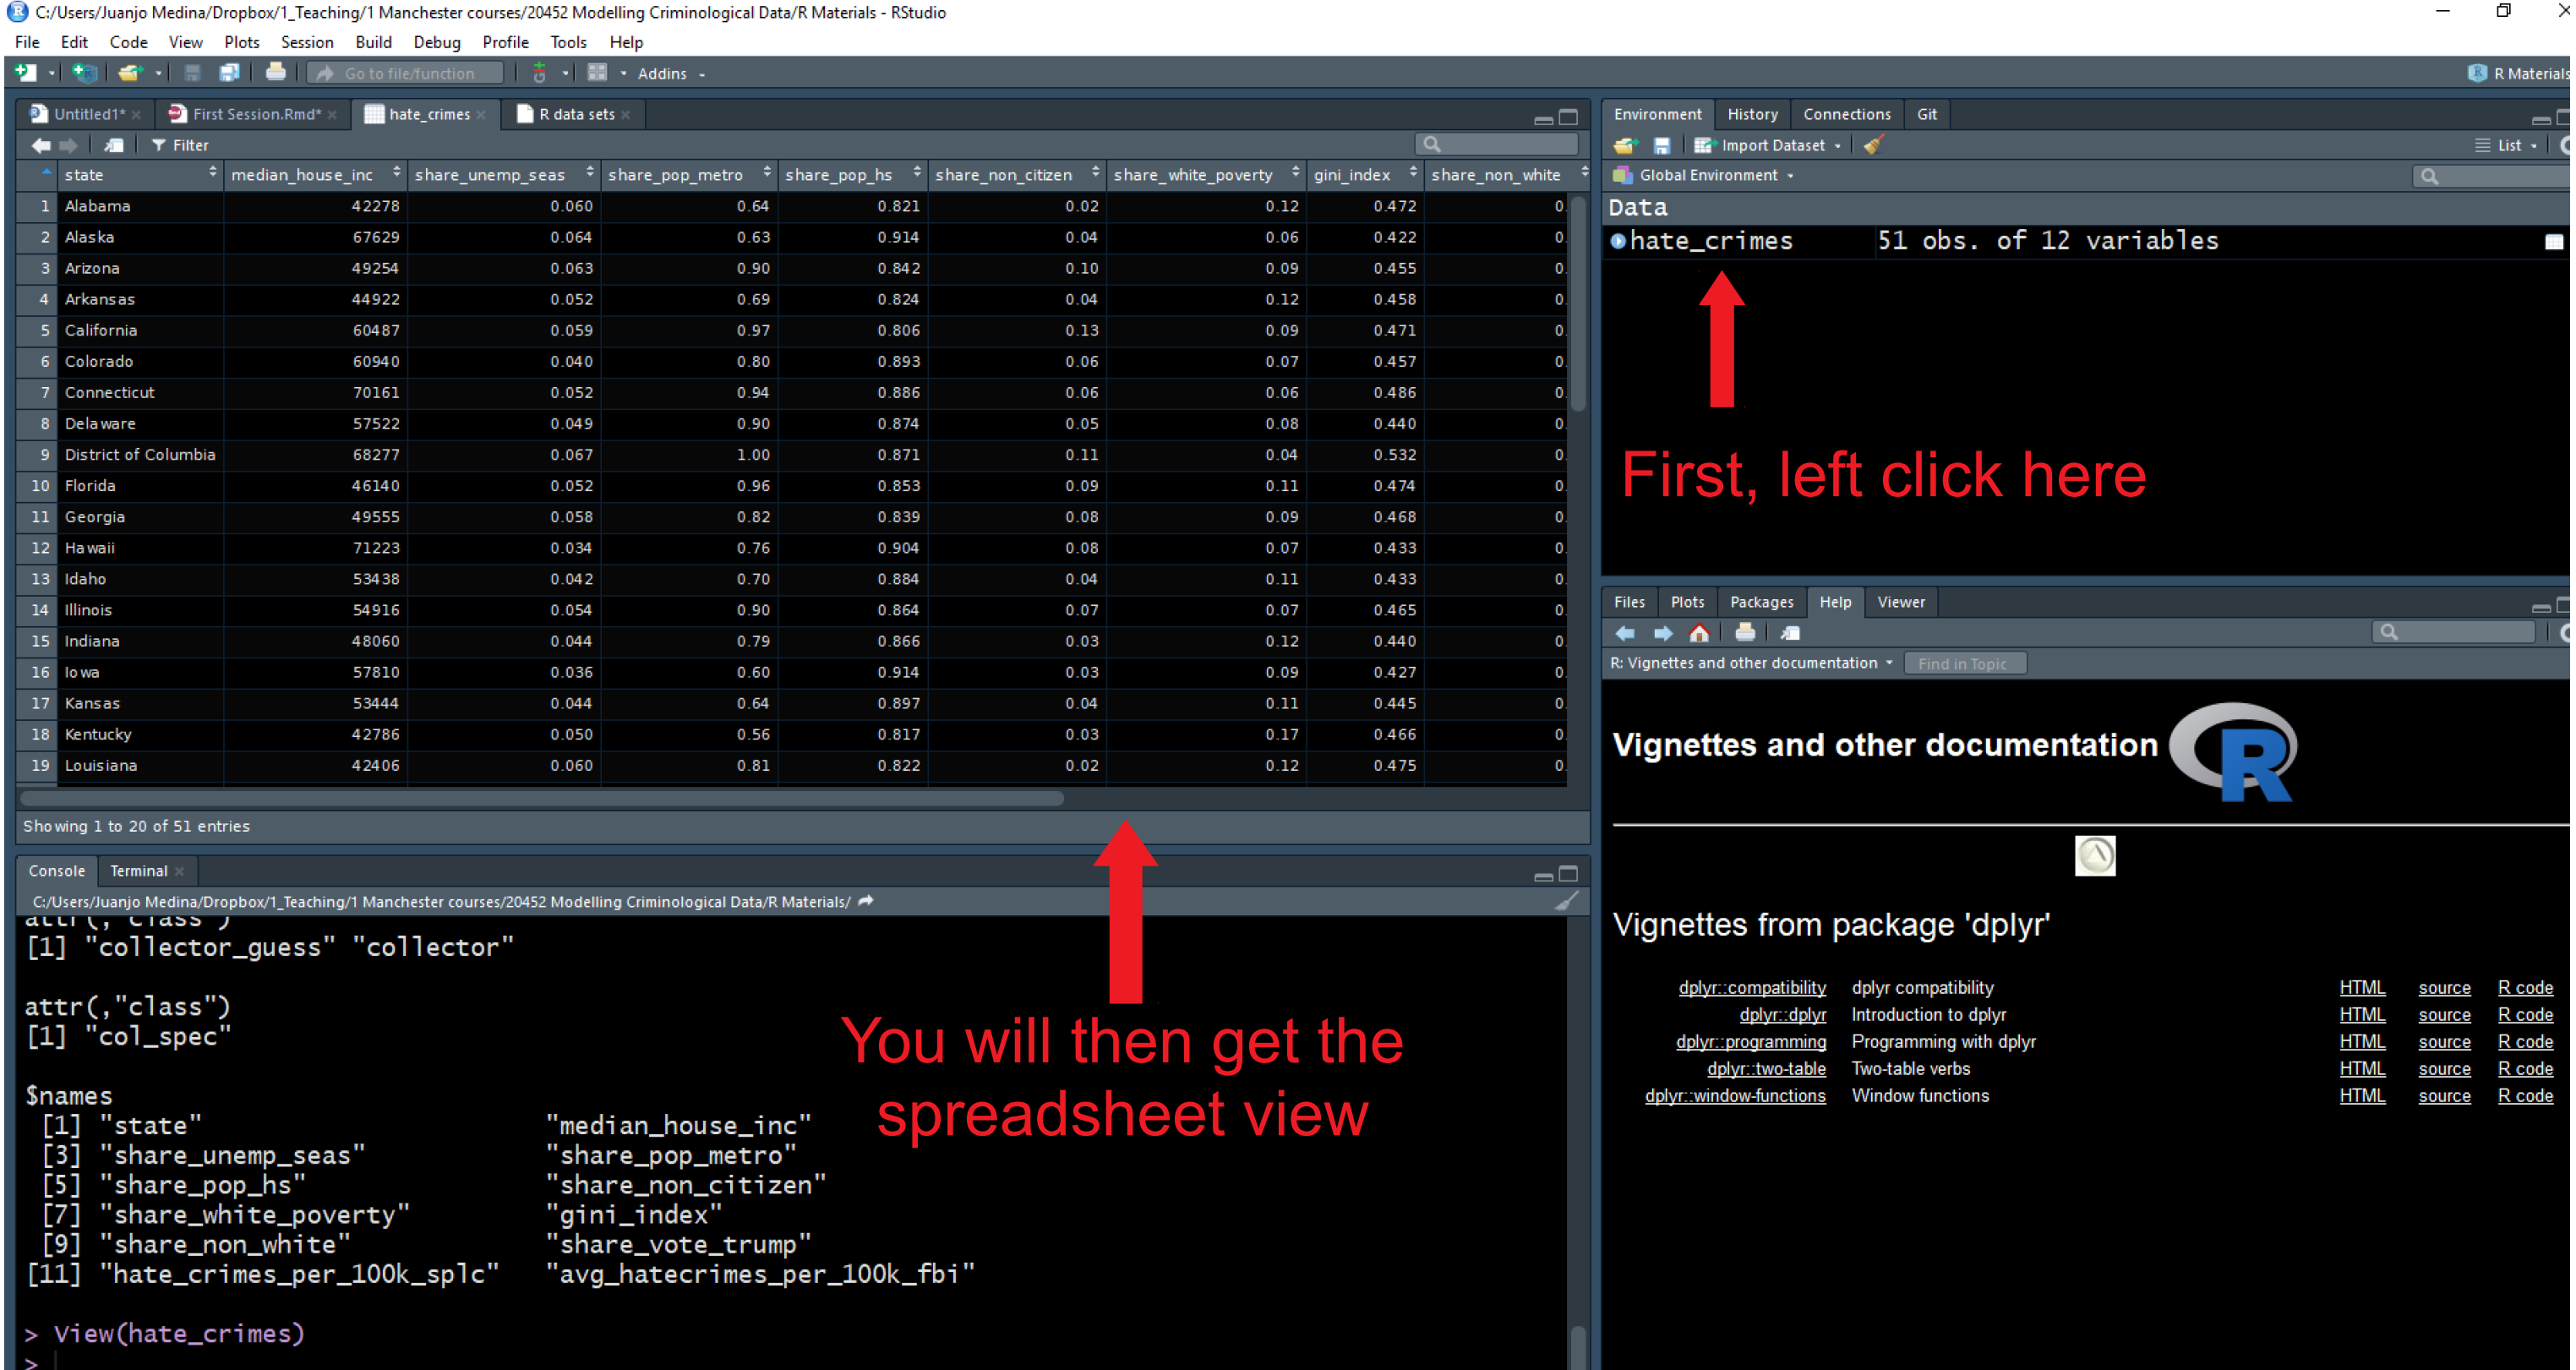
\includegraphics{imgs/dataview.png}

\#\#Exploring data

Ok, let's now have a quick look at the data. There are so many different
ways of producing summary stats for data stored in R that is impossible
to cover them all! We will just introduce a few functions that you may
find useful for summarising data. Before we do any of that it is
important you get a sense for what is available in this data set. Go to
the help tab and in the search box input the name of the data frame,
this will take you to the documentation for this data frame. Here you
can see a list of the available variables.

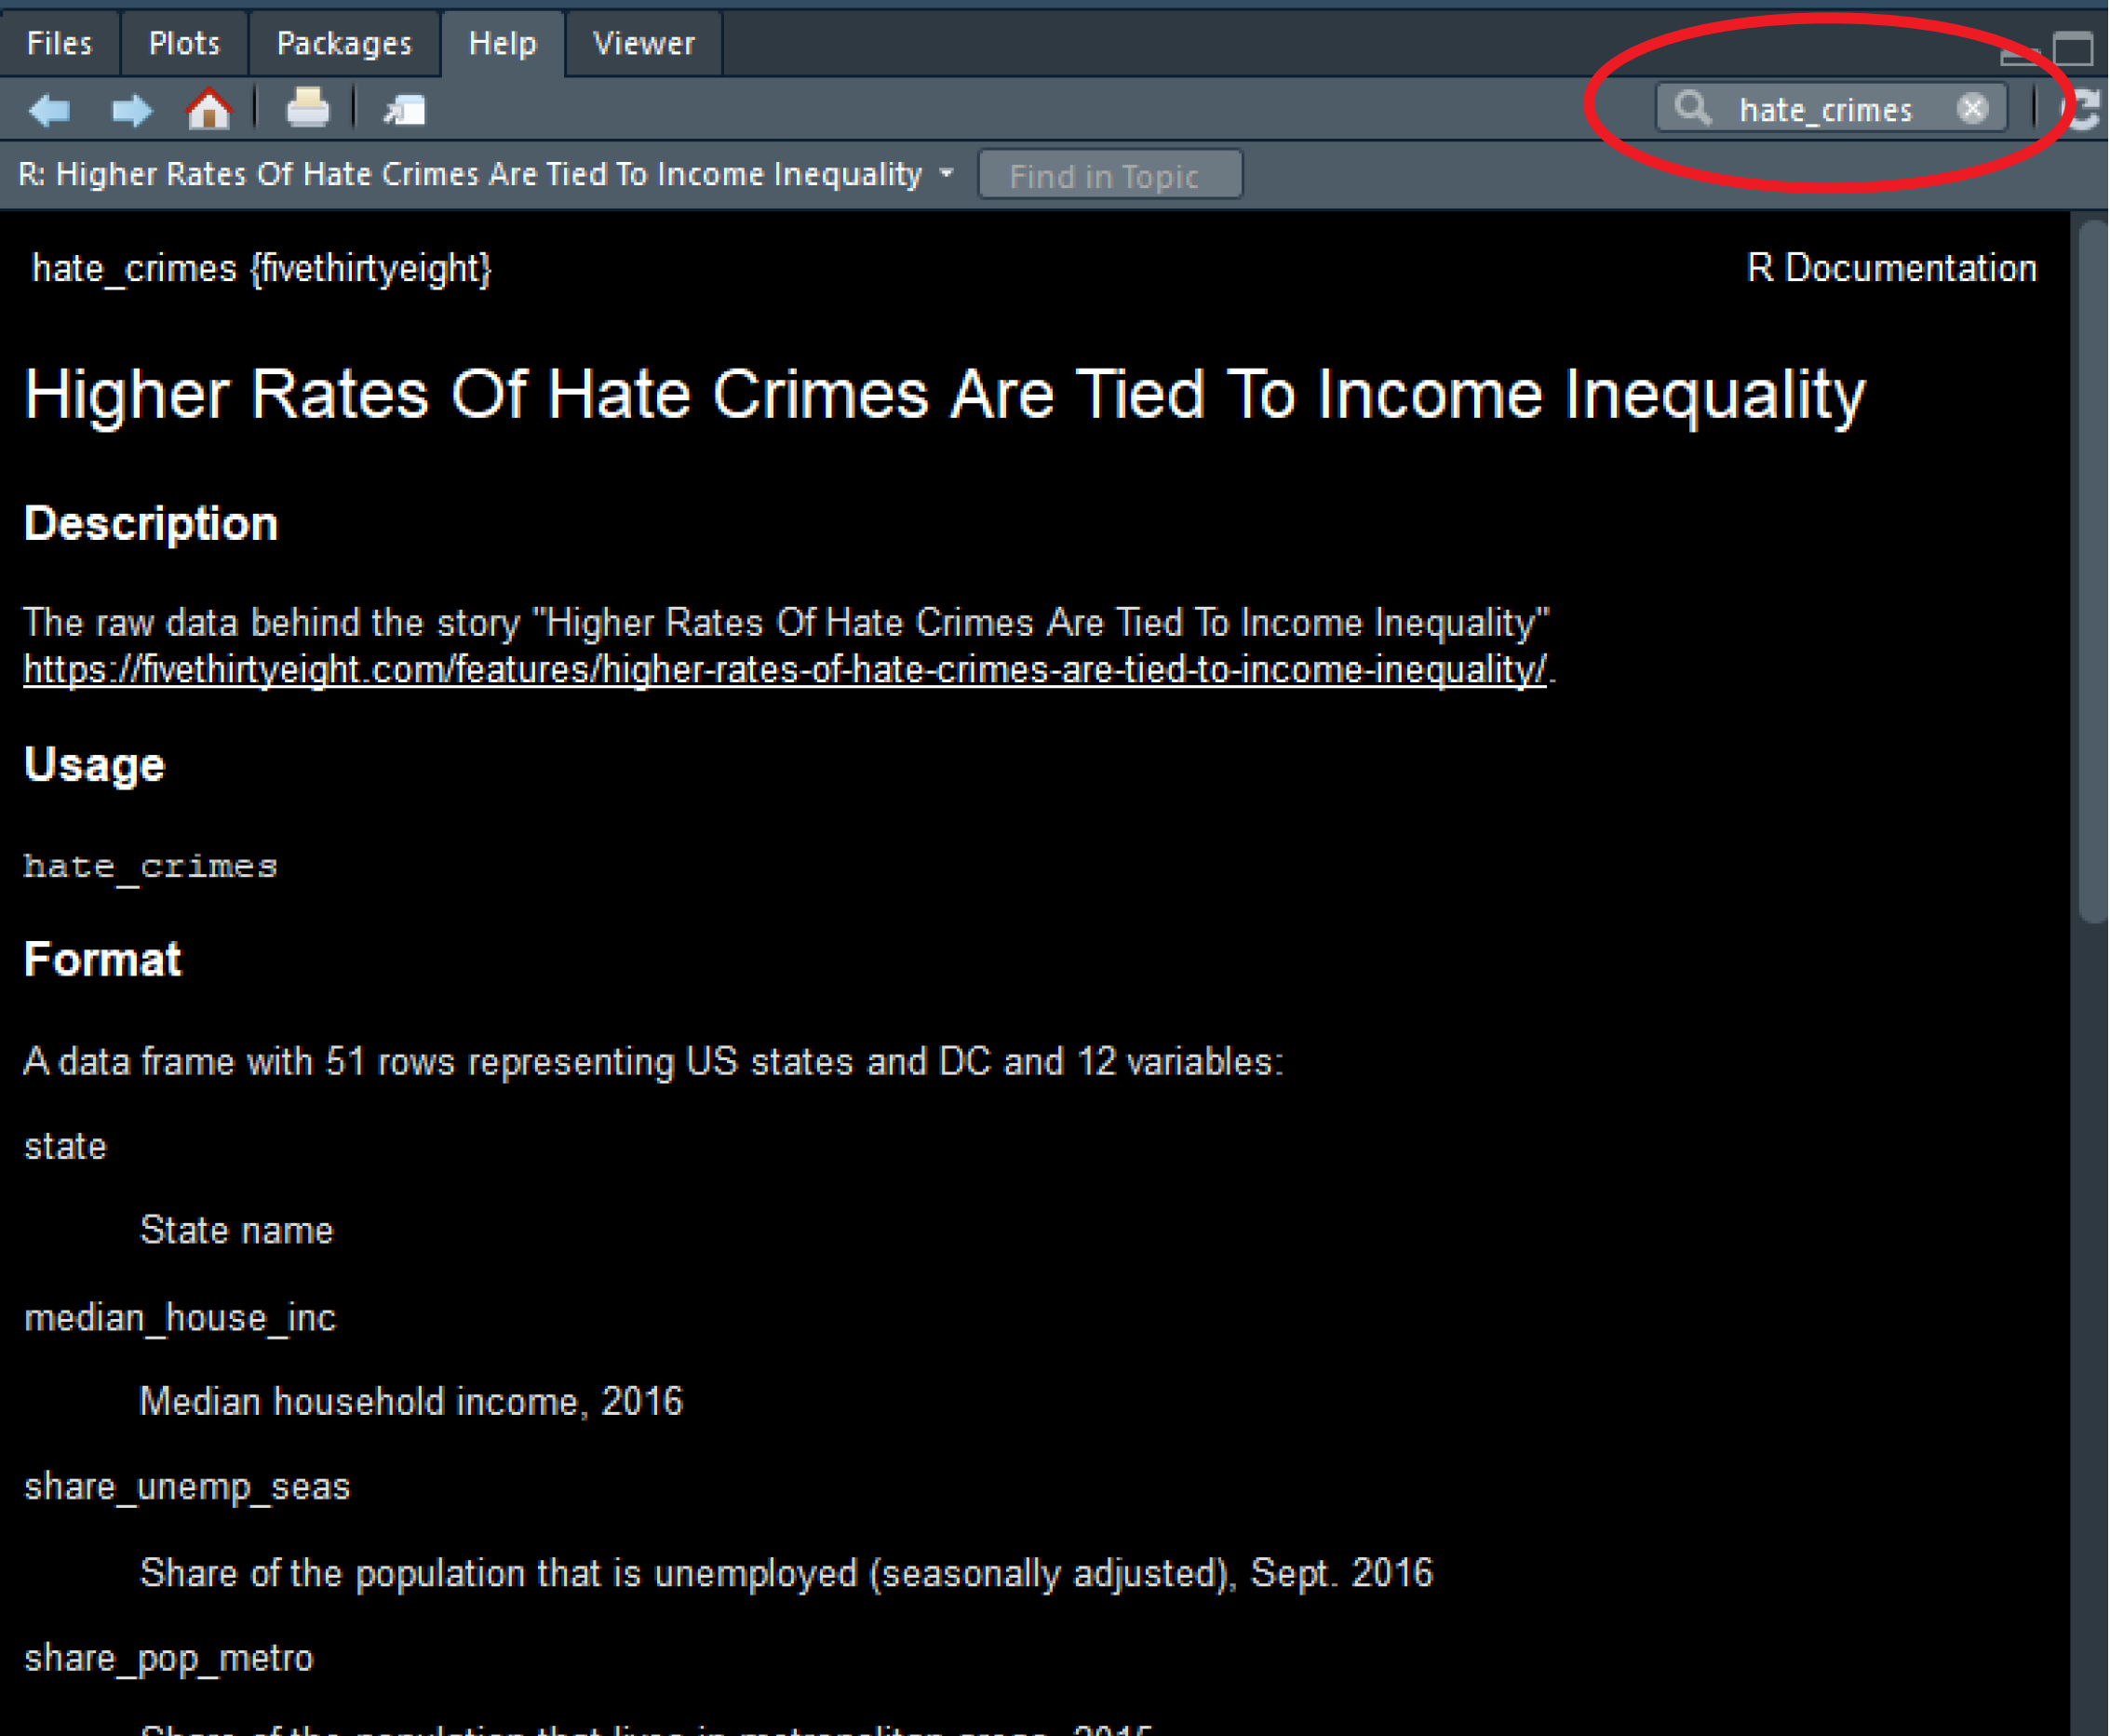
\includegraphics{imgs/codebook.png}

Let's start with the \emph{mean}. This function takes as an argument the
numeric variable for which you want to obtain the mean. Because of the
way that R works you cannot simply put the name of the variable you have
to tell R as well in which data frame is that variable located. To do
that you write the name of the data frame, the dollar sign, and then the
name of the variable you want to summarise. If you want to obtain the
mean of the variable that gives us the proportion of people that voted
for Donald Trump you can use the following expression:

\begin{Shaded}
\begin{Highlighting}[]
\KeywordTok{mean}\NormalTok{(hate_crimes}\OperatorTok{$}\NormalTok{share_vote_trump)}
\end{Highlighting}
\end{Shaded}

\begin{verbatim}
## [1] 0.49
\end{verbatim}

Another function you may want to use with numeric variables is
\texttt{summary()}:

\begin{Shaded}
\begin{Highlighting}[]
\KeywordTok{summary}\NormalTok{(hate_crimes}\OperatorTok{$}\NormalTok{share_vote_trump)}
\end{Highlighting}
\end{Shaded}

\begin{verbatim}
##    Min. 1st Qu.  Median    Mean 3rd Qu.    Max. 
##   0.040   0.415   0.490   0.490   0.575   0.700
\end{verbatim}

This gives you the five number summary (minimum, first quartile, median,
third quartile, and maximum, plus the mean and the count of missing
values if there are any).

You don't have to specify a variable you can ask for these summaries
from the whole data frame:

\begin{Shaded}
\begin{Highlighting}[]
\KeywordTok{summary}\NormalTok{(hate_crimes)}
\end{Highlighting}
\end{Shaded}

\begin{verbatim}
##     state           median_house_inc share_unemp_seas  share_pop_metro 
##  Length:51          Min.   :35521    Min.   :0.02800   Min.   :0.3100  
##  Class :character   1st Qu.:48657    1st Qu.:0.04200   1st Qu.:0.6300  
##  Mode  :character   Median :54916    Median :0.05100   Median :0.7900  
##                     Mean   :55224    Mean   :0.04957   Mean   :0.7502  
##                     3rd Qu.:60719    3rd Qu.:0.05750   3rd Qu.:0.8950  
##                     Max.   :76165    Max.   :0.07300   Max.   :1.0000  
##                                                                        
##   share_pop_hs    share_non_citizen share_white_poverty   gini_index    
##  Min.   :0.7990   Min.   :0.01000   Min.   :0.04000     Min.   :0.4190  
##  1st Qu.:0.8405   1st Qu.:0.03000   1st Qu.:0.07500     1st Qu.:0.4400  
##  Median :0.8740   Median :0.04500   Median :0.09000     Median :0.4540  
##  Mean   :0.8691   Mean   :0.05458   Mean   :0.09176     Mean   :0.4538  
##  3rd Qu.:0.8980   3rd Qu.:0.08000   3rd Qu.:0.10000     3rd Qu.:0.4665  
##  Max.   :0.9180   Max.   :0.13000   Max.   :0.17000     Max.   :0.5320  
##                   NA's   :3                                             
##  share_non_white  share_vote_trump hate_crimes_per_100k_splc
##  Min.   :0.0600   Min.   :0.040    Min.   :0.06745          
##  1st Qu.:0.1950   1st Qu.:0.415    1st Qu.:0.14271          
##  Median :0.2800   Median :0.490    Median :0.22620          
##  Mean   :0.3157   Mean   :0.490    Mean   :0.30409          
##  3rd Qu.:0.4200   3rd Qu.:0.575    3rd Qu.:0.35694          
##  Max.   :0.8100   Max.   :0.700    Max.   :1.52230          
##                                    NA's   :4                
##  avg_hatecrimes_per_100k_fbi
##  Min.   : 0.2669            
##  1st Qu.: 1.2931            
##  Median : 1.9871            
##  Mean   : 2.3676            
##  3rd Qu.: 3.1843            
##  Max.   :10.9535            
##  NA's   :1
\end{verbatim}

There are multiple ways of getting results in R. Particularly for basic
and intermediate-level statistical analysis many core functions and
packages can give you the answer that you are looking for. For example,
there are a variety of packages that allow you to look at summary
statistics using functions defined within those packages. You will need
to install these packages before you can use them.

I am only going to introduce one of them here \emph{skimr}. It is neat
and is maintained by one of my former stats teachers, the criminologist
Elin Waring. You will need to install it before anything else. Use the
code you have learnt to do so and then load it. I won't be providing you
the code for it, by now you should now how to do this.

Once you have loaded the \emph{skimr} package you can use it. Its main
function is \emph{skim}. Like \emph{summary} for data frames, skim
presents results for all the columns and the statistics will depend on
the class of the variable. However, the results are displayed and stored
in a nicer way -though we won't get into the details of this right now.

\begin{Shaded}
\begin{Highlighting}[]
\KeywordTok{skim}\NormalTok{(hate_crimes)}
\end{Highlighting}
\end{Shaded}

Skim summary statistics\\
n obs: 51\\
n variables: 12

Variable type: character

\begin{tabular}{l|l|l|l|l|l|l|l}
\hline
variable & missing & complete & n & min & max & empty & n\_unique\\
\hline
state & 0 & 51 & 51 & 4 & 20 & 0 & 51\\
\hline
\end{tabular}

Variable type: integer

\begin{tabular}{l|l|l|l|l|l|l|l|l|l|l}
\hline
variable & missing & complete & n & mean & sd & p0 & p25 & p50 & p75 & p100\\
\hline
median\_house\_inc & 0 & 51 & 51 & 55223.61 & 9208.48 & 35521 & 48657 & 54916 & 60719 & 76165\\
\hline
\end{tabular}

Variable type: numeric

\begin{tabular}{l|l|l|l|l|l|l|l|l|l|l}
\hline
variable & missing & complete & n & mean & sd & p0 & p25 & p50 & p75 & p100\\
\hline
avg\_hatecrimes\_per\_100k\_fbi & 1 & 50 & 51 & 2.37 & 1.71 & 0.27 & 1.29 & 1.99 & 3.18 & 10.95\\
\hline
gini\_index & 0 & 51 & 51 & 0.45 & 0.021 & 0.42 & 0.44 & 0.45 & 0.47 & 0.53\\
\hline
hate\_crimes\_per\_100k\_splc & 4 & 47 & 51 & 0.3 & 0.25 & 0.067 & 0.14 & 0.23 & 0.36 & 1.52\\
\hline
share\_non\_citizen & 3 & 48 & 51 & 0.055 & 0.031 & 0.01 & 0.03 & 0.045 & 0.08 & 0.13\\
\hline
share\_non\_white & 0 & 51 & 51 & 0.32 & 0.16 & 0.06 & 0.2 & 0.28 & 0.42 & 0.81\\
\hline
share\_pop\_hs & 0 & 51 & 51 & 0.87 & 0.034 & 0.8 & 0.84 & 0.87 & 0.9 & 0.92\\
\hline
share\_pop\_metro & 0 & 51 & 51 & 0.75 & 0.18 & 0.31 & 0.63 & 0.79 & 0.9 & 1\\
\hline
share\_unemp\_seas & 0 & 51 & 51 & 0.05 & 0.011 & 0.028 & 0.042 & 0.051 & 0.058 & 0.073\\
\hline
share\_vote\_trump & 0 & 51 & 51 & 0.49 & 0.12 & 0.04 & 0.41 & 0.49 & 0.57 & 0.7\\
\hline
share\_white\_poverty & 0 & 51 & 51 & 0.092 & 0.025 & 0.04 & 0.075 & 0.09 & 0.1 & 0.17\\
\hline
\end{tabular}

Apart from summary statistics, last semester we discussed a variety of
ways to graphically display variables. In week 3 we covered
scatterplots, a graphical device to show the relationship between two
quantitative variables. I don't know if you remember the amount of point
and click you had to do in Excel for getting this done. If not you can
review the notes
\href{https://rawgit.com/maczokni/MSCD/master/Lesson_3.html\#visualising-the-differences-between-groups}{here}.

There's also many different ways of producing graphics in R. In this
course we rely on a package called \emph{ggplot2}. It is already in the
clusters, but if you are using your own laptop will need to install it
first and then load it.

\begin{Shaded}
\begin{Highlighting}[]
\KeywordTok{library}\NormalTok{(ggplot2)}
\end{Highlighting}
\end{Shaded}

Then we will use one of its functions to create a scatterplot. Don't
worry about understanding this code below, we will have a whole session
on the ggplot function:

\begin{Shaded}
\begin{Highlighting}[]
\KeywordTok{ggplot}\NormalTok{(hate_crimes, }\KeywordTok{aes}\NormalTok{(}\DataTypeTok{x=}\NormalTok{share_vote_trump, }\DataTypeTok{y=}\NormalTok{avg_hatecrimes_per_100k_fbi)) }\OperatorTok{+}
\StringTok{    }\KeywordTok{geom_point}\NormalTok{(}\DataTypeTok{shape=}\DecValTok{1}\NormalTok{) }\OperatorTok{+}
\StringTok{     }\KeywordTok{geom_smooth}\NormalTok{(}\DataTypeTok{method=}\NormalTok{lm)}
\end{Highlighting}
\end{Shaded}

\begin{verbatim}
## Warning: Removed 1 rows containing non-finite values (stat_smooth).
\end{verbatim}

\begin{verbatim}
## Warning: Removed 1 rows containing missing values (geom_point).
\end{verbatim}

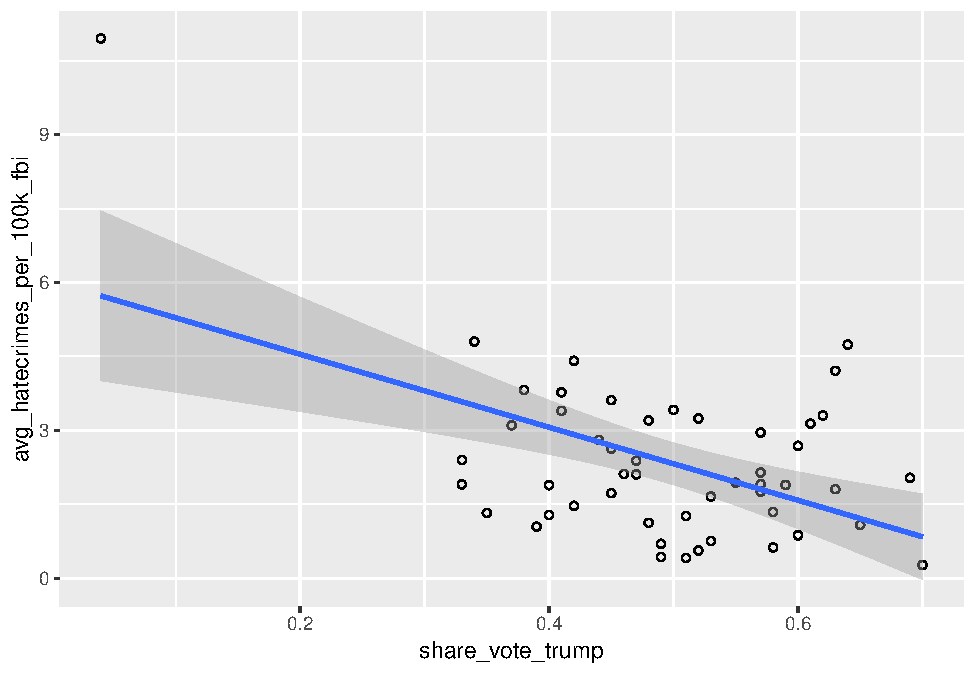
\includegraphics{01-intro_files/figure-latex/unnamed-chunk-34-1.pdf}

What do you think this graphic is telling you?

\#\#Quitting RStudio

At some point, you will quit your R/R Studio session. I know, hard to
visualise, right? Why would you want to do that? Anyhow, when that
happens R Studio will ask you a hard question: ``Save work space image
to bla bla bla/.RData?'' What to do? What does that even mean?

If you say ``yes'' what will happen is that all the objects you have in
your environment will be preserved, alongside the \emph{History} (which
you can access in the top right set of windows) listing all the
functions you have run within your session. So, next time you open this
project all will be there. If you think that what is \emph{real} is
those objects and that history, well then you may think that's what you
want to do.

Truth is what is real is your scripts and the data that your scripts use
as inputs. You don't need anything that is in your environment, because
you can recreate those things by re-running your scripts. I like keeping
things tidy, so when I am asked whether I want to save the image, my
answer is always no. Most long time users of R never save the workspace,
nor care about saving the history either. Remember what is real is your
scripts and the data.

Keep in mind though that you should not then panic if you open your next
R Studio session and you don't see any objects in your environment. The
good news is you can generate them quickly enough (if you really need
them) by re-running your scripts. I would suggest that at this point it
may be helpful for you to get into this habit as well. I suspect
otherwise you will be in week 9 of the semester and have an environment
full of garbage you don't really need.

What is more. I would suggest you go to the Tools drop down menu, select
Global Options, and make sure you select ``Never'' where it says ``Save
workspace''. Then click ``Apply''. This way you will never be asked to
save what is in your global environment when you terminate a session.

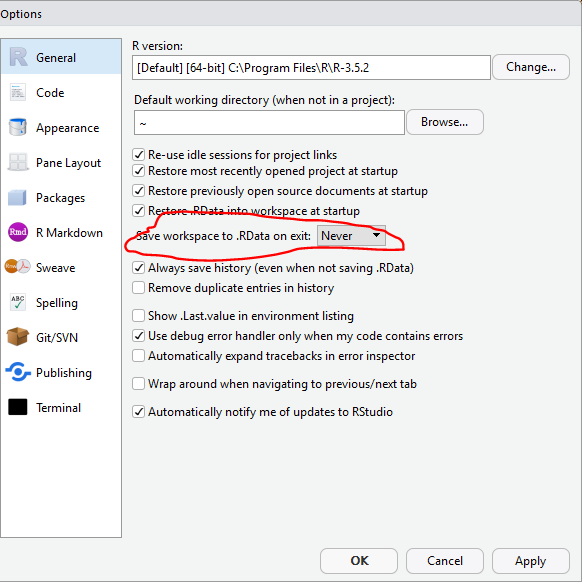
\includegraphics{imgs/neversave.PNG}

\#Causality in randomised experiments (Week 2)

\hypertarget{causality-in-social-sciences}{%
\section{Causality in social
sciences}\label{causality-in-social-sciences}}

In today's week we will refresh some of the themes you have explored in
previous research methods courses. We are going to talk specifically
about causality. This is one of the central concepts in empirical
research. We often do research because we want to make causal
inferences. We want to be in a position where we establish whether an
intervention or a social process is causally linked to crime or some
other relevant criminological outcome.

Making causal inferences typically involves making comparisons between
cases that have been subject to an intervention or that present some
sort of attribute that we think may have a causal effect to cases that
have not being subject to the causal process we are trying to establish.
But by your previous training, you should already know that not all kind
of comparisons are the same. In the first semester we discussed the
differeces between experimental and observational studies and we
established how this different kinds of research designs have a bearing
on your ability to make causal inference.

Let's think about a specific case so that this makes more sense. Is
there discrimination against former offenders in the labor market? In
other words, are offenders less likely to find employment after release
because of prejudice among employers? Or can we say that the fact that
former offenders are less likely to be in employment may be due to other
factors? Perhaps, they are less skilled. Perhaps they have less social
capital, people they know that can help them to get jobs or to learn
about job opportunities. Perhaps, they are less interested in finding
employment and more in
\href{https://www.youtube.com/watch?v=p47fEXGabaY}{living ``la vida
loca''}.

Only in comparisons when other things are equal you can make causal
inferences. It would only be fair to compare John, an ex-offender with a
high school degree and X number of personal connections and Y numbers of
professional experience, with Peter, a non-ex offender, with the same
educational and profesisonal credentials than John (and everything else
that matters when getting jobs also being equal between Peter and John).

How can you do that? How can you create situations when other things are
equal? Well, that's what courses in research design are oriented to
teach you. What is important for you to remember is that the way data
are generated, the way you do your study, will, of course, affect the
kind of interpretations that you make from your statistical comparisons.
And not all studies are created equal. Some research designs put you in
a better position than others to make causal inference.

You should have learnt by now that the
\href{https://link.springer.com/article/10.1007/s11292-005-3538-2}{``bronze''
standard} for establishing causality in the social sciences is the
randomized experiment. In a randomised trial, the researchers change the
causal variable of interest for a group using something like a coin
toss. As Angrist and Pischke (2015: xiii) highlight:

\emph{``By changing circumstances randomly, we make it highly likely
that the variable of interest is unrelated to the many other factors
determining the outcomes we mean to study\ldots{} Random manipulation
makes other things equal hold on average across the groups that did and
did not experience manipulation''}

So, say you want to establish whether arresting a perpetrator may have a
deterrent effect on subsequent domestic abuse. You could randomise,
basically use the equivalent of a lottery, to decide whether the police
officer is going to arrest the perpetrator or not and then compare those
you arrest with those you don't arrest. Because you are randomising your
treatment (the arrest) on average the treatment and the control group on
the long run should be fairly similar and any differences you observe
between them in the outcome of interest (domestic abuse recidivism) you
could link it to your intervention -if you are interested in the answer
to this you can read about it
\href{http://niccsa.org/uploads/file/f815aa02a0804639a53bb4a800952235/EFFECTSOFARRESTONINTIMATEPARTNERVIOLENCE.pdf}{here}.

In this session we will look at data from a randomised trial that tried
to establish whether there is discrimination in the labour market
against former offenders. In doing so, we will also learn various
functions used in R to read data, transform data, and to obtain summary
statistics for groups. We will also very quickly introduce a plotting
function used in R to generate graphics.

\hypertarget{getting-data-thanks-to-reproducibility}{%
\section{Getting data thanks to
reproducibility}\label{getting-data-thanks-to-reproducibility}}

Last week we introduced the notion of reproducible research and said
that using and publishing code (particularly if using open source tools
like R) is the way that
\href{https://osf.io/?gclid=EAIaIQobChMIq-jM6MuY2QIV7Z3tCh04vAycEAAYASAAEgLptPD_BwE}{many
researchers} around the world think that science ought to be done. This
way of operating makes research more open, more credible, and more
legitimate. It also means that we can more easily access the data used
in published research. For this session we are going to use the data
from \href{https://academic.oup.com/qje/article/133/1/191/4060073}{this}
and
\href{https://pubs.aeaweb.org/doi/pdfplus/10.1257/aer.p20171003}{this
paper}. In this research project, the authors tried to answer the
question of whether criminal antecendents and other personal
characteristics have an impact on access to employment.

\href{http://economics.rutgers.edu/people/626-amanda-agan}{Amanda Agan}
and
\href{https://www.law.umich.edu/FacultyBio/Pages/FacultyBio.aspx?FacID=sbstarr}{Sonja
Starr} developed a randomised experiment in which they created 15,220
fake resumes randomly generating these critical characteristics (such as
having a criminal record) and used these resumes to send online job
applications to low-skill, entry level job openings in New Jersey and
New York City. All the fictious applicants were male and about 21 to 22
years old. These kind of experiments are very common among researchers
that want to explore through these ``audits'' whether some personal
characteristics are discriminated against in the labor market.

Because Amanda Agan and Sonja Starr conformed to reproducibly standards
when doing their research we can access this data from the \emph{Harvard
Dataverse} (a repositoty for open research data). Click
\href{https://dataverse.harvard.edu/dataset.xhtml?persistentId=doi:10.7910/DVN/VPHMNT}{here}
to locate the data.

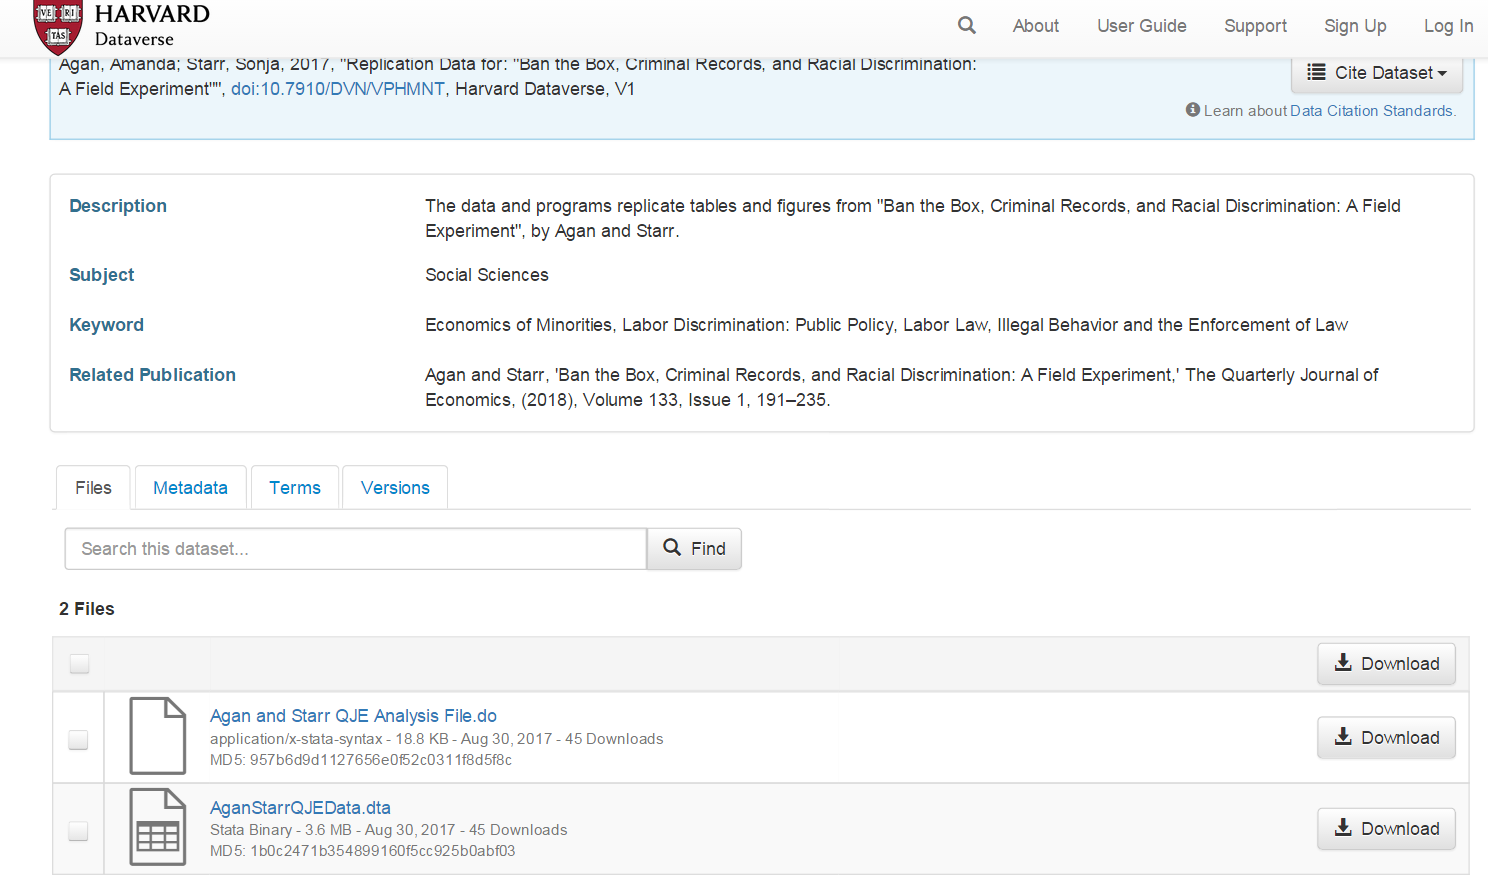
\includegraphics{imgs/harvarddataverse.PNG}

In this page you can see a download section and some files that can be
accessed. One of them contains analytical code pertaning to the study
and the other contains the data. You also see a link called
\textbf{metadata}. Metadata is data about data, it simply provides you
with some information about the data. If you clink in metadata you will
see at the bottom a reference to the software the authors used (STATA).
So we know these files are in \href{https://www.stata.com/}{STATA}
proprietary format. Let's download the data file and then read the data
into R.

You could just click download and then place the file in your project
directory. Alternatively, and preferably, you may want to use code to
make your whole work more reproducible. Think of it this way, every time
you click or use drop down menus you are doing things that others cannot
reproduce because there won't be a written record of your steps. You
will need though to do some clicking for finding out the required url
you will use for writing your code. The file we want is the
AganStarrQJEData.dta. Click in the name of this file. You will be taken
to another webpage. On it you will see the download url. Copy and paste
this url in your code below.

\begin{Shaded}
\begin{Highlighting}[]
\CommentTok{#First, let's create an object with the link, paste the copied address here:}
\NormalTok{data_url <-}\StringTok{ "https://dataverse.harvard.edu/api/access/datafile/3036350"}
\end{Highlighting}
\end{Shaded}

This data file is a STATA .dta file in our working directory. To read
STATA files we will need the \emph{haven} package. If you don't have it
you will need to install it. And then load it.

\begin{Shaded}
\begin{Highlighting}[]
\KeywordTok{library}\NormalTok{(haven)}
\CommentTok{#Now we can use the read_dta function, within this function we will}
\CommentTok{#pass an argument, url, specifying to the read_dta function the need to}
\CommentTok{#make a url connection. The url function takes as an argument the url}
\CommentTok{#we are using and that we encoded in the data_url object in our case.}
\NormalTok{banbox <-}\StringTok{ }\KeywordTok{read_dta}\NormalTok{(}\KeywordTok{url}\NormalTok{(data_url))}
\end{Highlighting}
\end{Shaded}

You should now have a new object in your global environment. Check the
dimensions of the file.

\hypertarget{getting-a-sense-for-your-data}{%
\section{Getting a sense for your
data}\label{getting-a-sense-for-your-data}}

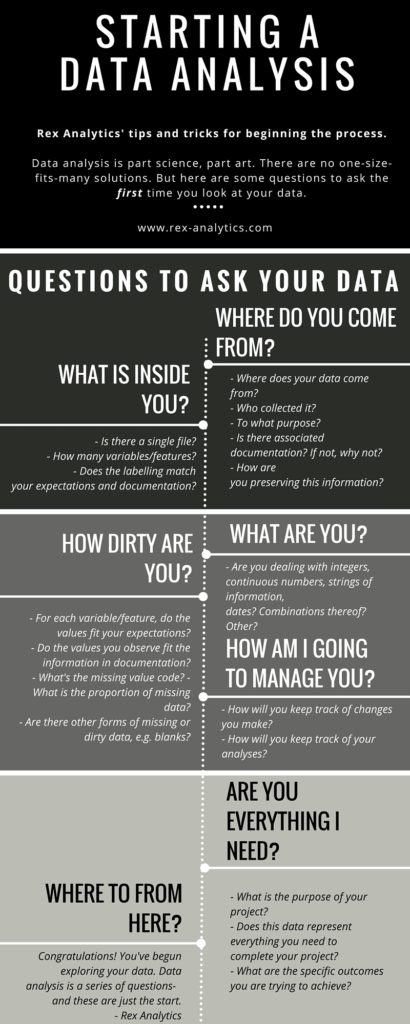
\includegraphics{imgs/firstlookatdata.jpg}

What is the first thing you need to ask yourself when you look at a
dataset? Data are often too big to look at the whole thing. It is almost
always impossible to eyeball the entire dataset and see what you have in
terms of interesting patterns or potential problems. It is often a case
of information overload and we want to be able to extract what is
relevant and important about it. But where do you start?
\href{http://rex-analytics.com/data-analysis-questions-to-ask-the-first-time/}{Here}
you can find a brief but very useful overview put together by Steph de
Silva. Read it before we carry on.

As Mara Averick (somebody you want to follow in twitter at
\citet{dataanndme} if you want to be in top of R related resources)
suggests this also makes for good relationship advice!


\includegraphics{imgs/relationships.png}

Here we are going to introduce a few functions that will help you to
start making sense for what you have just downloaded. Summarising the
data is the first step in any analysis and it is also used for finding
out potential problems with the data. Regarding the latter you want to
look out for: missing values; values outside the expected range (e.g.,
someone aged 200 years); values that seem to be in the wrong units;
mislabelled variables; or variables that seem to be the wrong class
(e.g., a quantitative variable encoded as a factor). Lets start by the
basic things you always look first in a datasets.

You can see in the Environment window that banbox has 14813 observations
(rows) of 62 variables (columns). You can also obtain this information
using code. Here you want the \textbf{DIM}ensions of the dataframe (the
number of rows and columns) so you use the \texttt{dim()} function:

\begin{Shaded}
\begin{Highlighting}[]
\KeywordTok{dim}\NormalTok{(banbox)}
\end{Highlighting}
\end{Shaded}

\begin{verbatim}
## [1] 14813    62
\end{verbatim}

Looking at this information will help you to diagnose whether there was
any trouble getting your data into R (e.g., imagine you know there
should be more cases or more variables). You may also want to have a
look at the names of the columns using the \texttt{names()} function. We
will see the names of the variables.

\begin{Shaded}
\begin{Highlighting}[]
\KeywordTok{names}\NormalTok{(banbox)}
\end{Highlighting}
\end{Shaded}

\begin{verbatim}
##  [1] "nj"                   "nyc"                  "app_date_d"          
##  [4] "pre"                  "post"                 "storeid"             
##  [7] "chain_id"             "center"               "crimbox"             
## [10] "crime"                "drugcrime"            "propertycrime"       
## [13] "ged"                  "empgap"               "white"               
## [16] "black"                "remover"              "noncomplier_store"   
## [19] "balanced"             "response"             "response_date_d"     
## [22] "daystoresponse"       "interview"            "cogroup_comb"        
## [25] "cogroup_njnyc"        "post_cogroup_njnyc"   "white_cogroup_njnyc" 
## [28] "ged_cogroup_njnyc"    "empgap_cogroup_njnyc" "box_white"           
## [31] "pre_white"            "post_white"           "white_nj"            
## [34] "post_remover_ged"     "post_ged"             "remover_ged"         
## [37] "post_remover_empgap"  "post_empgap"          "remover_empgap"      
## [40] "post_remover_white"   "post_remover"         "remover_white"       
## [43] "raerror"              "retail"               "num_stores"          
## [46] "avg_salesvolume"      "avg_num_employees"    "retail_white"        
## [49] "retail_post"          "retail_post_white"    "percblack"           
## [52] "percwhite"            "tot_crime_rate"       "nocrimbox"           
## [55] "nocrime_box"          "nocrime_pre"          "response_white"      
## [58] "response_black"       "response_ged"         "response_hsd"        
## [61] "response_empgap"      "response_noempgap"
\end{verbatim}

As you may notice, these names may be hard to interpret. If you open the
dataset in the data viewer of RStudio you will see that each column has
a variable name and underneath a longer and more meaninful
\emph{variable label} that tells you what each variable means.

You also want to understand what the banbox object actually is. You can
do that using the \emph{class()} function:

\begin{Shaded}
\begin{Highlighting}[]
\KeywordTok{class}\NormalTok{(banbox)}
\end{Highlighting}
\end{Shaded}

\begin{verbatim}
## [1] "tbl_df"     "tbl"        "data.frame"
\end{verbatim}

What does tbl stands for? It refers to \textbf{tibbles}. This is
essentially a new type of data structure introduced into R. Tibbles
\emph{are} data frames. That's what the class() function also says, but
they introduce some tweaks to make life easier.

The R language has been around for a while and sometimes things that
made sense a couple of decades ago, make less sense now. A number of
programmers are trying to create code that is more modern and more
useful today. They are doing this by introducing a set of packages that
speak to each other in order to modernise R without breaking existing
code. You can think of it as a modern dialect of R. This set of packages
is called the \textbf{tidyverse}. Tibbles are dataframes that have been
optimised within this new set of packages. You can read a bit more about
tibbles \href{http://r4ds.had.co.nz/tibbles.html}{here}.

You can also look at the class of each individual column. As discussed,
class of the variable lets us know if its an integer (number) or factor.

To get the class of one variable, you pass it to the \texttt{class()}
function. For example:

\begin{Shaded}
\begin{Highlighting}[]
\KeywordTok{class}\NormalTok{(banbox}\OperatorTok{$}\NormalTok{crime)}
\end{Highlighting}
\end{Shaded}

\begin{verbatim}
## [1] "haven_labelled"
\end{verbatim}

\begin{Shaded}
\begin{Highlighting}[]
\KeywordTok{class}\NormalTok{(banbox}\OperatorTok{$}\NormalTok{num_stores)}
\end{Highlighting}
\end{Shaded}

\begin{verbatim}
## [1] "numeric"
\end{verbatim}

We talked about numeric vectors in week one. It is simply a collection
of numbers. But what is a labelled vector? This is a new type of vector
introduced by the \emph{haven} package. Labelled vectors are categorical
variables that have labels. Go to the \emph{Environment} panel and left
click in the banbox object. This should open the data browser in the top
left quadrant of RStudio.

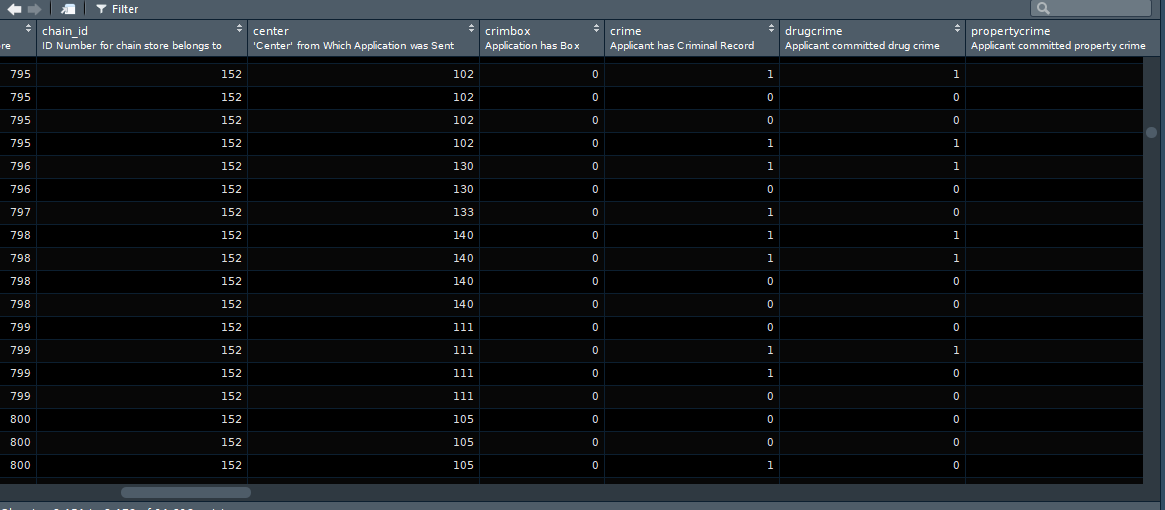
\includegraphics{imgs/dataview_causality.png}

If you look carefully you will see that the various columns that include
categorical variables only contain numbers. In many statistical
environments, such as STATA or SPSS, this is a common standard. The
variables have a numeric value for each observation and then each of
these numeric values is associated with a label. This kind of made sense
when computer memory was an issue - for this was an efficient way of
saving resources. These days it makes perhaps less sense. But labelled
vectors give you a chance to reproduce data from other statistical
environments without losing any fidelity in the import process. See what
happens if we try to summarise this labelled vector. We will use the
\emph{table()} to provide a count of observations on the various valid
values of the \emph{crime} variable. It is a function to obtain your
frequency distribution.

\begin{Shaded}
\begin{Highlighting}[]
\KeywordTok{table}\NormalTok{(banbox}\OperatorTok{$}\NormalTok{crime)}
\end{Highlighting}
\end{Shaded}

\begin{verbatim}
## 
##    0    1 
## 7323 7490
\end{verbatim}

So, we see that we have 7490 observations classed as 1 and 7323 classed
as 2. If only we knew what those numbers represent! Well, we actually
do. We will use the \emph{attributes()} function to see the different
``compartments''" within your ``box'', your object.

\begin{Shaded}
\begin{Highlighting}[]
\KeywordTok{attributes}\NormalTok{(banbox}\OperatorTok{$}\NormalTok{crime)}
\end{Highlighting}
\end{Shaded}

\begin{verbatim}
## $label
## [1] "Applicant has Criminal Record"
## 
## $format.stata
## [1] "%9.0g"
## 
## $class
## [1] "haven_labelled"
## 
## $labels
## No Crime    Crime 
##        0        1
\end{verbatim}

So this object has different compartments. The first one is called label
and it provides a description of what the variable measures. This is
what you saw in the RStudio data viewer earlier. The second compartment
explains the original format in which it was. The third one identifies
the class of the vector. Whereas the final one \emph{labels} provides
the labels that allows us to identify what the meaning of 0 and 1 mean
in this context.

Last week we said that many R functions expect factors when you have
categorical data, so typically after you import data into R you may want
to coerce your labelled vectors into factors. To do that you need to use
the \emph{as\_factor()} function of the \emph{haven} package. Let's see
how we do that.

\begin{Shaded}
\begin{Highlighting}[]
\CommentTok{#This code asks R to create a new column in your banbox tibble}
\CommentTok{#that is going to be called crime_f. Typically, when you alter}
\CommentTok{#variables you can to create a new one so that the original gets}
\CommentTok{#preserved in case you do something wrong. Then we use the}
\CommentTok{#as_factor() function to explain to R that what we want to do}
\CommentTok{#is to get the original crime variable and mutate it into }
\CommentTok{#a factor, this resulting factor is what will be stored in}
\CommentTok{#the new column.}
\NormalTok{banbox}\OperatorTok{$}\NormalTok{crime_f <-}\StringTok{ }\KeywordTok{as_factor}\NormalTok{(banbox}\OperatorTok{$}\NormalTok{crime)}
\end{Highlighting}
\end{Shaded}

You will see now that you have 63 variables in your dataset, look at the
environment to check. Let's explore the new variable we have created
(you can also look for the new variable in the data browser and see how
it looks different to the original crime variable):

\begin{Shaded}
\begin{Highlighting}[]
\KeywordTok{class}\NormalTok{(banbox}\OperatorTok{$}\NormalTok{crime_f)}
\end{Highlighting}
\end{Shaded}

\begin{verbatim}
## [1] "factor"
\end{verbatim}

\begin{Shaded}
\begin{Highlighting}[]
\KeywordTok{table}\NormalTok{(banbox}\OperatorTok{$}\NormalTok{crime_f)}
\end{Highlighting}
\end{Shaded}

\begin{verbatim}
## 
## No Crime    Crime 
##     7323     7490
\end{verbatim}

\begin{Shaded}
\begin{Highlighting}[]
\KeywordTok{attributes}\NormalTok{(banbox}\OperatorTok{$}\NormalTok{crime_f)}
\end{Highlighting}
\end{Shaded}

\begin{verbatim}
## $levels
## [1] "No Crime" "Crime"   
## 
## $class
## [1] "factor"
## 
## $label
## [1] "Applicant has Criminal Record"
\end{verbatim}

So far we have a looked at single columns in your dataframe one at the
time. But there is a way that you can apply a function to all elements
of a vector (list or dataframe). You can use the functions
\texttt{sapply()}, \texttt{lapply()}, and \texttt{mapply()} . To find
out more about when to use each one see
\href{https://www.r-bloggers.com/using-apply-sapply-lapply-in-r/}{here}.

For example, we can use the \texttt{lapply()} function to look at each
column and get its class. To do so, we have to pass two arguments to the
\texttt{lapply()} function, the first is the name of the dataframe, to
tell it what to look through, and the second is the function we want it
to apply to every column of that function.

So we want to type ``lapply('' + ``name of dataframe'' + ``,'' + ``name
of function'' + ``)''

Which is:

\begin{Shaded}
\begin{Highlighting}[]
\KeywordTok{lapply}\NormalTok{(banbox, class)}
\end{Highlighting}
\end{Shaded}

As you can see many variables are classed as labelled. This is common
with survey data. Many of the questions in social surveys measure the
answers as categorical variables (e.g., these are nominal or ordinal
level measures). In fact, with this dataset there are many variables
that are encoded as numeric that really aren't. Welcome to real world
data, where things can be a bit messy and need tidying!

See for example the variable black:

\begin{Shaded}
\begin{Highlighting}[]
\KeywordTok{class}\NormalTok{(banbox}\OperatorTok{$}\NormalTok{black)}
\end{Highlighting}
\end{Shaded}

\begin{verbatim}
## [1] "numeric"
\end{verbatim}

\begin{Shaded}
\begin{Highlighting}[]
\KeywordTok{table}\NormalTok{(banbox}\OperatorTok{$}\NormalTok{black)}
\end{Highlighting}
\end{Shaded}

\begin{verbatim}
## 
##    0    1 
## 7406 7407
\end{verbatim}

We know that this variable measures whether someone is black or not.
When people use 0 and 1 to code binary responses, typically they use a 1
to denote a positive response, a yes. So, I think it is fair to assume
that a 1 here means the respondent is black. Because this variable is of
class numeric we cannot simply use as\_factor to assign the pre-existing
labels and create a new factor. In this case we don't have preexisting
labels, since this is not a labelled vector. So what can we do to tidy
this variable? We'll we need to do some further work.

\begin{Shaded}
\begin{Highlighting}[]
\CommentTok{#We will use a slightly different function as.factor()}
\NormalTok{banbox}\OperatorTok{$}\NormalTok{black_f <-}\StringTok{ }\KeywordTok{as.factor}\NormalTok{(banbox}\OperatorTok{$}\NormalTok{black)}
\CommentTok{#You can check that the resulting column is a factor}
\KeywordTok{class}\NormalTok{(banbox}\OperatorTok{$}\NormalTok{black_f)}
\end{Highlighting}
\end{Shaded}

\begin{verbatim}
## [1] "factor"
\end{verbatim}

\begin{Shaded}
\begin{Highlighting}[]
\CommentTok{#But if you print the frequency distribution you will see the}
\CommentTok{#data are still presented in relation to 0 and 1}
\KeywordTok{table}\NormalTok{(banbox}\OperatorTok{$}\NormalTok{black_f)}
\end{Highlighting}
\end{Shaded}

\begin{verbatim}
## 
##    0    1 
## 7406 7407
\end{verbatim}

\begin{Shaded}
\begin{Highlighting}[]
\CommentTok{#You can use the levels function to see the levels, the }
\CommentTok{#categories, in your factor}
\KeywordTok{levels}\NormalTok{(banbox}\OperatorTok{$}\NormalTok{black_f)}
\end{Highlighting}
\end{Shaded}

\begin{verbatim}
## [1] "0" "1"
\end{verbatim}

So, all we have done is create a new column that is a factor but still
refers to 0 and 1. If we assume (rightly) that 1 mean black we have 7407
black applicants. Of course, it makes sense we only get 0 and 1 here.
What else could R do? This is not a labelled vector, so there is no way
for R to know that 0 and 1 mean anything other than 0 and 1, which is
why those are the levels is using. But now that we have the factor we
can rename those levels. We can use the following code to do just that:

\begin{Shaded}
\begin{Highlighting}[]
\CommentTok{#We are using the levels function to access them and change}
\CommentTok{#them to the levels we specify with the c() function. Be}
\CommentTok{#careful here, because the order we specify here will map }
\CommentTok{#out to the order of the existing levels. So given that 1 is }
\CommentTok{#black and black is the second level (as shown when printing}
\CommentTok{#the results above) you want to make sure that in the c()}
\CommentTok{#you write black as the second level.}
\KeywordTok{levels}\NormalTok{(banbox}\OperatorTok{$}\NormalTok{black_f) <-}\StringTok{ }\KeywordTok{c}\NormalTok{(}\StringTok{"White"}\NormalTok{, }\StringTok{"Black"}\NormalTok{)}
\KeywordTok{table}\NormalTok{(banbox}\OperatorTok{$}\NormalTok{black_f)}
\end{Highlighting}
\end{Shaded}

\begin{verbatim}
## 
## White Black 
##  7406  7407
\end{verbatim}

This gives you an idea of the kind of transformations you often want to
perform to make your data more useful for your purposes. But let's keep
looking at functions you can use to explore your dataset.

You can, for example, use the \texttt{head()} function if you just want
to visualise the values for the first few cases in your dataset. The
next code for example ask for the values for the first two cases. If you
want a different number to be shown you just need to change the number
you are passing as an argument.

\begin{Shaded}
\begin{Highlighting}[]
\KeywordTok{head}\NormalTok{(banbox, }\DecValTok{2}\NormalTok{)}
\end{Highlighting}
\end{Shaded}

In the same way you could look at the last two cases in your dataset
using \texttt{tail()}:

\begin{Shaded}
\begin{Highlighting}[]
\KeywordTok{tail}\NormalTok{(banbox, }\DecValTok{2}\NormalTok{)}
\end{Highlighting}
\end{Shaded}

It is good practice to do this to ensure R has read the data correctly
and there's nothing terribly wrong with your dataset. If you have access
to STATA you can open the original file in STATA and check if there are
any discrepancies, for example. Glimpsing your data in this way can also
give you a first impression for what the data looks like.

One thing you may also want to do is to see if there are any
\textbf{missing values}. For that we can use the \texttt{is.na()}
function. Missing values in R are coded as NA. The code below, for
example, asks for NA values for the variable \emph{response\_black} in
the \emph{banbox} object for observations 1 to 10:

\begin{Shaded}
\begin{Highlighting}[]
\KeywordTok{is.na}\NormalTok{(banbox}\OperatorTok{$}\NormalTok{response_black[}\DecValTok{1}\OperatorTok{:}\DecValTok{10}\NormalTok{])}
\end{Highlighting}
\end{Shaded}

\begin{verbatim}
##  [1] FALSE  TRUE  TRUE FALSE FALSE  TRUE  TRUE  TRUE FALSE  TRUE
\end{verbatim}

The result is a logical vector that tells us if it is true that there is
missing (NA) data for each of those first ten observations. You can see
that there are 6 observations out of those 10 that have missing values
for this variable.

\begin{Shaded}
\begin{Highlighting}[]
\KeywordTok{sum}\NormalTok{(}\KeywordTok{is.na}\NormalTok{(banbox}\OperatorTok{$}\NormalTok{response_black)) }
\end{Highlighting}
\end{Shaded}

\begin{verbatim}
## [1] 7406
\end{verbatim}

This is asking R to sum how many cases are TRUE NA in this variable.
When reading a logical vector as the one we are creating, R will treat
the FALSE elements as 0s and the TRUE elements as 1s. So basically the
sum() function will count the number of TRUE cases returned by the
is.na() function.

You can use a bit of a hack to get the proportion of missing cases
instead of the count:

\begin{Shaded}
\begin{Highlighting}[]
\KeywordTok{mean}\NormalTok{(}\KeywordTok{is.na}\NormalTok{(banbox}\OperatorTok{$}\NormalTok{response_black))}
\end{Highlighting}
\end{Shaded}

\begin{verbatim}
## [1] 0.4999662
\end{verbatim}

This code is exploiting the mathematical fact that the mean of binary
outcomes (0 or 1) gives you the proportion of 1s in your data. If you
see more than 5\% of the cases declared as NA, you need to start
thinking about the implications of this. Beware of formulaic application
of rules of thumb such as this though! In this case, we know that 49\%\%
of the observations have missing values in this variable. When you see
things like this the first thing to do is to look at the codebook or
documenation to try to get some clues as to why there are so many
missing cases. With survey data you often have questions that are simply
not asked to everybody, so it's not necessarily that something went very
wrong with the data collection, but simply that the variable in question
was only used with a subset of the sample.

There is a whole field of statistics devoted to doing analysis when
missing data is a problem. R has extensive capabilities for dealing with
missing data -see for example
\href{http://www.crcpress.com/product/isbn/9781439868249}{here}. For the
purpose of this introductory course, we only explain how to do analysis
that ignore missing data. This is often referred to a
\textbf{full/complete case analysis}, because you only use observations
for which you have full information in all the variables you employ. You
would cover techniques for dealing with this sort of issues in more
advanced courses.

\hypertarget{data-wrangling-with-dplyr}{%
\section{Data wrangling with dplyr}\label{data-wrangling-with-dplyr}}

The data analysis workflow has a number of stages. The diagram below
(produced by Hadley Wickham) is a nice illustration of this process:

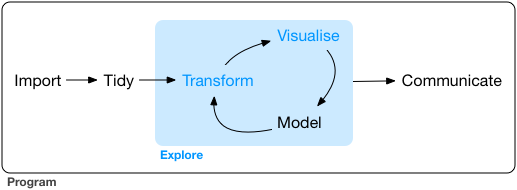
\includegraphics{imgs/data-science-explore.png}

We have started to see different ways of bringing data into R. And we
have also started to see how we can explore our data. It is now time we
start discussing one of the following stages, \textbf{transform}. A good
deal of time and effort in data analysis is devoted to this. You get
your data and then you have to do some transformations to it so that you
can answer the questions you want to address in your research.

R offers a great deal of flexibility in how to do this kind of thing,
Here we are going to illustrate some of the functionality of the
\emph{dplyr} package for data carpentry. This package is part of the
tydiverse and it aims to provide a friendly and modern take on how to
work with dataframes (or tibbles) in R. It offers, as the authors of the
package put it, ``a flexible grammar of data manipulation''.

Dplyr aims to provide a function for each basic verbs of data
manipulation:

\begin{itemize}
\tightlist
\item
  \emph{filter()} to select cases based on their values.
\item
  \emph{arrange()} to reorder the cases.
\item
  \emph{select()} and \emph{rename()} to select variables based on their
  names.
\item
  \emph{mutate()} and \emph{transmute()} to add new variables that are
  functions of existing variables.
\item
  \emph{summarise()} to condense multiple values to a single value.
\item
  \emph{sample\_n()} and \emph{sample\_frac()} to take random samples.
\end{itemize}

In this session we will introduce and practice some of these. But we
won't have time to cover everything. There is, however, a very nice set
of vignettes for this package in the help files, so you can try to go
through those if you want a greater degree of detail or more practice.

Now let's load the package:

\begin{Shaded}
\begin{Highlighting}[]
\KeywordTok{library}\NormalTok{(dplyr)}
\end{Highlighting}
\end{Shaded}

\begin{verbatim}
## 
## Attaching package: 'dplyr'
\end{verbatim}

\begin{verbatim}
## The following objects are masked from 'package:stats':
## 
##     filter, lag
\end{verbatim}

\begin{verbatim}
## The following objects are masked from 'package:base':
## 
##     intersect, setdiff, setequal, union
\end{verbatim}

Notice that when you run this package you get a series of warnings. It
is telling us that some functions from certain packages are being
``masked''. One the things with a language like R is that sometimes
packages introduce functions that have the same name than others that
are already loaded into your session. When that happens the newly loaded
ones will over-ride the previous ones. You can still use them but you
will have to refer to them explicitly. Otherwise R will assume you are
using the function most recently loaded:

\begin{Shaded}
\begin{Highlighting}[]
\CommentTok{#Example:}
\CommentTok{#If you use load dplyr and then invoke the *filter()* function}
\CommentTok{#R will assume you are using the filter function from dplyr}
\CommentTok{#rather than the *filter()* function that exist in the *stats*}
\CommentTok{#package, which is part of the basic installation of R. If }
\CommentTok{#after loading dplyr you want to use the filter function from}
\CommentTok{#the stats package you will have to invoke it like this:}
\NormalTok{stats}\OperatorTok{::}\KeywordTok{filter}\NormalTok{()}
\CommentTok{#Notice the grammar, first you write the name of the package,}
\CommentTok{#then colon twice, and then the name of the function. Don't }
\CommentTok{#run this code. You would need to pass some valid arguments}
\CommentTok{#for this to produce meaningful results.}
\end{Highlighting}
\end{Shaded}

\hypertarget{using-dplyr-single-verbs}{%
\section{Using dplyr single verbs}\label{using-dplyr-single-verbs}}

One of the first operations you may want to carry out when working with
dataframes is to subset them based on values of particular variables.
Say we want to replicate the results reported by Agan and Starr in 2017.
In this earlier paper, these researchers only used data from the period
prior to the introduction of Ban the Box legislation and only used data
from businesses that asked about criminal records in their online
applications. How can we recreate this dataset?

For this kind of operations we use the \emph{filter()} function. Like
all single verbs in dplyr, the first argument is the tibble (or data
frame). The second and subsequent arguments refer to variables within
that data frame, selecting rows where the expression is TRUE.

Ok, so if we look at the dataset we can see that there is a variable
called crimbox that identifies applications that require information
about criminal antecedents and there is a variable called pre that
identifies whether the application was sent before the legislation was
introduced. In this dataset the value 1 is being used to denote positive
responses. So, if we want to create the 2017 dataset we would start by
selecting only data where the value in these two variables equals 1.

\begin{Shaded}
\begin{Highlighting}[]
\CommentTok{#We will store the results of filtering the data in a new }
\CommentTok{#object that I am calling aer (short for the name of the }
\CommentTok{#journal in which the paper was published)}

\NormalTok{aer2017<-}\StringTok{ }\KeywordTok{filter}\NormalTok{(banbox, crimbox }\OperatorTok{==}\StringTok{ }\DecValTok{1}\NormalTok{, pre }\OperatorTok{==}\StringTok{ }\DecValTok{1}\NormalTok{)}
\end{Highlighting}
\end{Shaded}

Notice that the number of cases equals the number of cases reported by
the authors in their 2017 paper. That's cool! So far we are replicating
with same results.

You may have noticed in the code above that I wrote ``==''" instead of
``=''. Logical operators in R are not written exactly the same way than
in normal practice. Keep this in mind when you get error messages from
running your code. Often the source of your error may be that you are
writing the logical operators the wrong way (as far as R is concerned).
Look \href{https://www.statmethods.net/management/operators.html}{here}
for valid logic operators in R.

Sometimes you may want to select only a few variables. Earlier we said
than real life data may have hundreds of variables and only a few of
those may be relevant for your analysis. Say you only want ``crime'',
``ged'' (a ged is a high school equivalence diploma rather than a proper
high school diploma and is sometimes seen as inferior), ``empgap'' (a
gap year on employment), ``black\_f'', ``response'', and
``daystoresponse'' from this dataset. For this kind of operations you
use the \emph{select()} function.

The syntax of this funciton is easy. First we name the dataframe object
(aer2017) and then we list the variables. The order in which we list the
variables within the select function will determine the order in which
those columns appear in the new dataframe we are creating. So this is a
handy function to use if you want to change the order of your columns
for some reason. Since I am pretty confident I am not making a mistake I
will transform the original ``aer2017'' tibble rather than creating an
entirely new object.

\begin{Shaded}
\begin{Highlighting}[]
\NormalTok{aer2017 <-}\StringTok{ }\KeywordTok{select}\NormalTok{(aer2017, crime, ged, empgap, black_f, response, daystoresponse)}
\end{Highlighting}
\end{Shaded}

If you now look at the global environment you will see that the
``aer2017'' tibble has reduced in size and now only has 6 columns. If
you view the data you will see these are the 6 variables we selected.

\hypertarget{using-dplyr-for-grouped-operations}{%
\section{Using dplyr for grouped
operations}\label{using-dplyr-for-grouped-operations}}

So far we have used dplyr sinle verbs for ungrouped operations. But we
can also use some of the functionality of dplyr for obtaining answers to
questions that relate to groups of cases within our dataframe. Imagine
that you want to know if applicants with a criminal record are less
likely to receive a positive response from employers. How could you
figure that one out? For answering this kind of questions we can use the
\emph{group\_by()} function in conjunction with other dplyr functions.
In particular we are going to look at the \emph{summarise} function.

\begin{Shaded}
\begin{Highlighting}[]
\CommentTok{#First we group the observations by criminal record in a new}
\CommentTok{#object, by using as_factor in the call to the crime variable}
\CommentTok{#the results will be labelled later on (even though we are}
\CommentTok{#not changing the crime variable in the aer2017 dataframe. Keep}
\CommentTok{#in mind we are using as_factor because the column crime is}
\CommentTok{#a labelled vector rather than a factor or a character vector,}
\CommentTok{#and we do this to aid interpretation (it is easier to}
\CommentTok{#interpret labels than 0 and 1).}
\NormalTok{by_antecedents <-}\StringTok{ }\KeywordTok{group_by}\NormalTok{(aer2017, }\KeywordTok{as_factor}\NormalTok{(crime))}
\CommentTok{#Then we run the summarise function to provide some useful}
\CommentTok{#summaries of the groups we are using: the number of cases}
\CommentTok{#and the mean of the response variable}
\NormalTok{results <-}\StringTok{ }\KeywordTok{summarise}\NormalTok{(by_antecedents,}
  \DataTypeTok{count =} \KeywordTok{n}\NormalTok{(),}
  \DataTypeTok{outcome =} \KeywordTok{mean}\NormalTok{(response, }\DataTypeTok{na.rm =} \OtherTok{TRUE}\NormalTok{))}
\CommentTok{#autoprint the results stored in the newly created object}
\NormalTok{results}
\end{Highlighting}
\end{Shaded}

\begin{verbatim}
## # A tibble: 2 x 3
##   `as_factor(crime)` count outcome
##   <fct>              <int>   <dbl>
## 1 No Crime            1319  0.136 
## 2 Crime               1336  0.0846
\end{verbatim}

Let's look at the code in the summarise function above. First we are
asking R to place the results in an object we are calling results. Then
we are specifying that we want to group the data in the way we specified
in our group\_by() function before, that is by criminal record. Then we
pass two arguments. Each of these arguments is creating a new variable
in the resulting object called ``results''. The first variable we are
creating is called \emph{count} by saying this equals n() we are
specifying to R that this new variable simply counts the number of cases
in each of the grouping categories. The second variable we are creating
is called \emph{outcome} and to compute this variable we are asking R to
compute the mean of the variable response for each of the two groups of
applicants (those with records, those without). Remember that the
variable response in the ``aer2017'' dataframe was coded as numeric
variable, even though in truth is categorical in nature (there was a
response, or not, from the employers). It doesn't really matter. Taking
the mean of a binary variable in this case is mathematically equivalent
to computing a proportion as we discussed earlier.

So, what we see here is that about 13.6\% of applicants with no criminal
record received a positive response from the employers, whereas only 8\%
of those with criminal records did receive such a response. Given that
the asignation of a criminal record was randomised to the applicants,
there's a pretty good chance that no other
\href{https://en.wikipedia.org/wiki/Confounding}{\textbf{confounders}}
are influencing this outcome. And that is the beauty of randomised
experiments. You may be in a position to make stronger claims about your
results.

\emph{HOMEWORK 1:} \emph{Use what we have learned so far to see if there
is an interaction effect between race and criminal records. That is,
what would happen if we compare 4 groups whites with no records, whites
with records, blacks with no records, and blacks with records. What do
you think? Is there an interaction effect? In other words, is the impact
of having a criminal record more accentuated for either of the two
racial groups? Be ready to answer these questions before you attempt the
Blackboard test}

\hypertarget{making-comparisons-with-numerical-outcomes}{%
\section{Making comparisons with numerical
outcomes}\label{making-comparisons-with-numerical-outcomes}}

We have been looking at relationships so far between categorical
variables, specifically between having a criminal record (yes or no),
race (black or white), and receiving a positive response from employers
(yes or no). Often we may be interested in looking at the impact of a
factor on a numerical outcome. In the banbox object we have such an
outcome measured by the researchers. The variable daystoresponse tells
us how long it took the employers to provide a positive response. Let's
look at this variable:

\begin{Shaded}
\begin{Highlighting}[]
\KeywordTok{summary}\NormalTok{(banbox}\OperatorTok{$}\NormalTok{daystoresponse)}
\end{Highlighting}
\end{Shaded}

\begin{verbatim}
##    Min. 1st Qu.  Median    Mean 3rd Qu.    Max.    NA's 
##    0.00    3.00   10.00   19.48   28.00  153.00   14361
\end{verbatim}

The summary() function provides some useful stats for numerical
variables. We obtain the minimum and maximum value, the 25th percentile,
the median, the mean, the 75th percentile, and the number of missing
data (NA). You can see the number of missing data here is massive. Most
cases have missing data on this variable. Clearly this is a function of,
first and foremost, the fact that the number of days to receive a
positive response will only be collected in cases where there was a
positive response. But even accounting for that, it is clear that this
information is also missing in many cases that received a positive
response. So given all of this, we need to be very careful when
interpreting this variable. Yet, because it is the only numeric variable
here we will use it to illustrate some handy functions.

We could do as before and get results by groups. Let's look at the
impact of race on days to response:

\begin{Shaded}
\begin{Highlighting}[]
\NormalTok{by_race <-}\StringTok{ }\KeywordTok{group_by}\NormalTok{(banbox, black_f)}
\NormalTok{results_}\DecValTok{3}\NormalTok{ <-}\StringTok{ }\KeywordTok{summarise}\NormalTok{(by_race,}
  \DataTypeTok{avg_delay =} \KeywordTok{mean}\NormalTok{(daystoresponse, }\DataTypeTok{na.rm =} \OtherTok{TRUE}\NormalTok{))}
\NormalTok{results_}\DecValTok{3}
\end{Highlighting}
\end{Shaded}

\begin{verbatim}
## # A tibble: 2 x 2
##   black_f avg_delay
##   <fct>       <dbl>
## 1 White        18.7
## 2 Black        20.4
\end{verbatim}

But we could also try to represent these differences graphically. The
problem with comparing groups on quantitative variables using numerical
summaries such as the mean, is that these comparisons hide more than
they show. We want to see the full distribution, not just the mean. For
this we are going to use ggplot2 the main graphical package we will use
this semester. We won't get into the details of this package or what the
code below means, but just try to run it. We will cover graphics in R in
the next section. This is just a taster for it.

\begin{Shaded}
\begin{Highlighting}[]
\KeywordTok{library}\NormalTok{(ggplot2)}
\KeywordTok{ggplot}\NormalTok{(banbox, }\KeywordTok{aes}\NormalTok{(}\DataTypeTok{y =}\NormalTok{ daystoresponse, }\DataTypeTok{x =}\NormalTok{ black_f)) }\OperatorTok{+}\StringTok{ }
\StringTok{  }\KeywordTok{geom_boxplot}\NormalTok{() }
\end{Highlighting}
\end{Shaded}

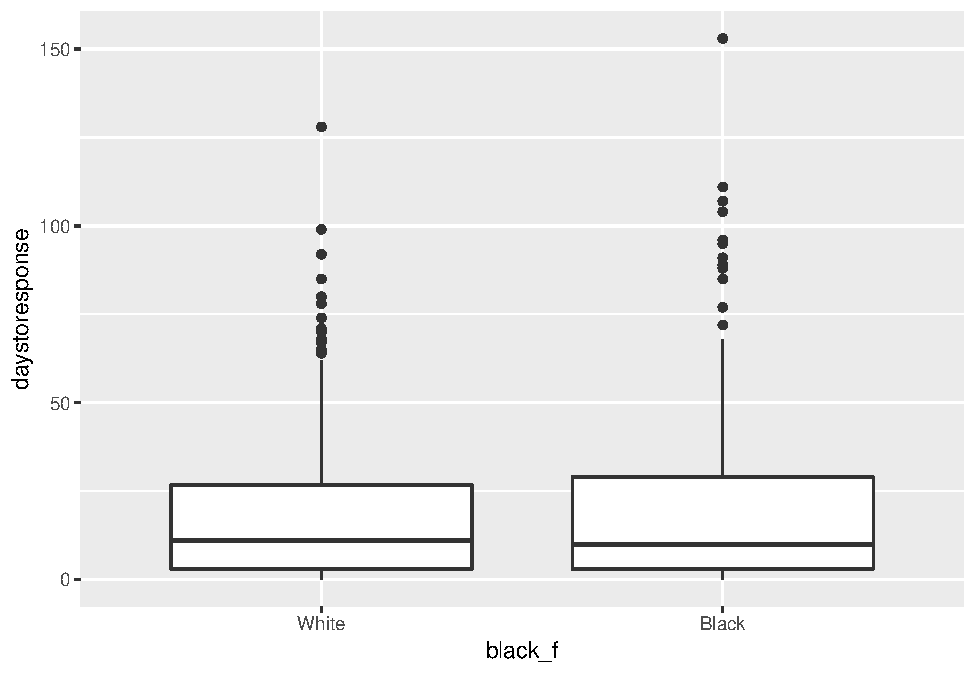
\includegraphics{02-causality_files/figure-latex/unnamed-chunk-29-1.pdf}

Watch
\href{https://www.khanacademy.org/math/probability/data-distributions-a1/box--whisker-plots-a1/v/reading-box-and-whisker-plots}{this
video} and see if you can interpret the results portrayed here. What do
you think?

\emph{Homework 2: For this course unit you need to write a coursework
assignment in which you will use data from a social survey to explore
relationships between various variables.}

\emph{Specifically, you will be allowed to use. So you will need to pick
one of them and then select a topic (of those listed below) to explore
with each of these surveys:} \emph{- The 2014 wave of the European
Social Survey, which you can access
\href{http://www.europeansocialsurvey.org/data/download.html?r=5}{here}
and explore \href{http://nesstar.ess.nsd.uib.no/webview/}{here}. From
this dataset you will be able to explore the following topic:
``Perception of an association between crime and immigration\emph{ }-
The 2013-2014 Crime Survey for England and Wales (the Teaching Dataset
version) which you can access
\href{https://discover.ukdataservice.ac.uk/catalogue/?sn=7911\&type=Data\%20catalogue}{here}
or explore \href{http://nesstar.ukdataservice.ac.uk/webview/}{here}.
From this dataset you will need to focus on one of two topics''violent
victimisation``,''perceptions of antisocial behaviour``, or''confidende
in the police".}

\textbf{As part of this week homework you need to let us know which
survey and which topic you want to focus on for your coursework
assignment}. \emph{Think about which of these topics appeals the most to
you when making your decision. Be ready to answer questions about this
when starting the Blackboard test}.

\emph{You can explore the datasets and what other variables are
available. For your coursework you will need to identify other variables
in these surveys that you think may be associated or helpful to
understand why people vary in worry of crime, attitudes toward
punishment, etc. At this point you don't need to identify those other
variables, but you may find it useful to explore what's available in
those datasets using NESSTAR (a guide for how to use NESSTAR is
available
\href{http://nesstar.com/help/4.0/webview/getting-started/getting-to-know-nesstar-webview.html}{here})and
the existing documentation for those studies}

\begin{verbatim}
## [1] "C/C/C/C/C/en_GB.UTF-8"
\end{verbatim}

\#Data visualisation with R (Week 3)

\#\#Introduction

A picture is worth a thousand words; when presenting and interpreting
data this basic idea also applies. There has been, indeed, a growing
shift in data analysis toward more visual approaches to both
interpretation and dissemination of numerical analysis. Part of the new
data revolution consists in the mixing of ideas from visualisation of
statistical analysis and visual design. Indeed data visualisation is one
of the most interesting areas of development in the field.

Good graphics not only help researchers to make their data easier to
understand by the general public. They are also a useful way for
understanding the data ourselves. In many ways it is very often a more
intuitive way to understand patterns in our data than trying to look at
numerical results presented in a tabular form.

Recent research has revealed that papers which have good graphics are
perceived as overall more clear and more interesting, and their authors
perceived as smarter (see \href{https://vimeo.com/181771433}{this
presentation})

The preparation for this session includes many great resources on
visualising quantitative information, and if you have not had time to go
thorugh them, I recommend that you take some time to do so.

As with other aspects of R, there are a number of core functions that
can be used to produced graphics. However these offer limited
possibilities for building graphs.

The package we will be using throughout this tutorial is
\texttt{ggplot2}. The aim of ggplot is to implement the
\href{http://www.springer.com/statistics/computational+statistics/book/978-0-387-24544-7}{grammar
of graphics}. The \texttt{ggplot2} package has excellent online
\href{http://ggplot2.org/}{documentation}.

If you don't already have the package installed, you will need to do so
using the \texttt{install.packages()} function.

You will then need to load up the package

\begin{Shaded}
\begin{Highlighting}[]
\KeywordTok{library}\NormalTok{(ggplot2)                                  }
\end{Highlighting}
\end{Shaded}

The grammar of graphics defines various components of the graphic. Some
of the most important are:

-\textbf{The data}: For using \texttt{ggplot2} the data has to be stored
as a data frame

-\textbf{The geoms}: They describe the objects that represent the data
(e.g., points, lines, polygons, etc.).

-\textbf{The aesthetics}: They describe the visual characteristics that
represent data (e.g., position, size, colour, shape, transparency).

-\textbf{Facets}: They describe how data is split into subsets and
displayed as multiple small graphs.

-\textbf{Stats}: They describe statistical transformations that
typically summarise data.

\#\#Anatomy of a plot

Essentially the philosophy behind this as that all graphics are made up
of layers. The package ggplot2 is based on the grammar of graphics, the
idea that you can build every graph from the same few components: a data
set, a set of geoms---visual marks that represent data points, and a
coordinate system.

Take this example (all taken from \emph{Wickham, H. (2010). A layered
grammar of graphics. Journal of Computational and Graphical Statistics,
19(1), 3-28.})

You have a table such as:

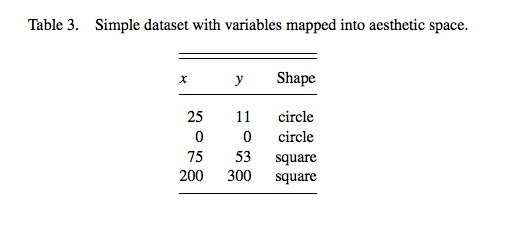
\includegraphics{imgs/table.png}

You then want to plot this. To do so, you want to create a plot that
combines the following layers:

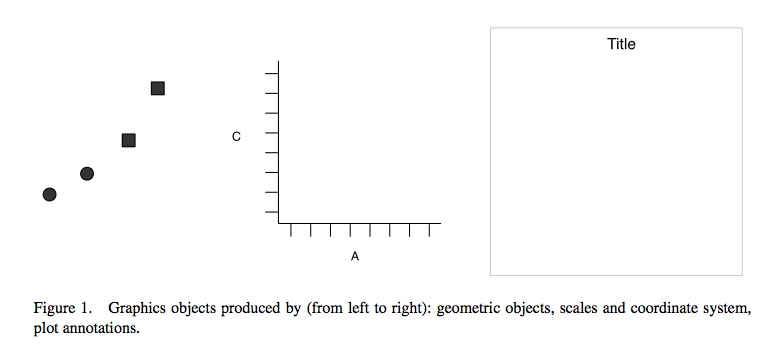
\includegraphics{imgs/layers.png}

This will result in a final plot:

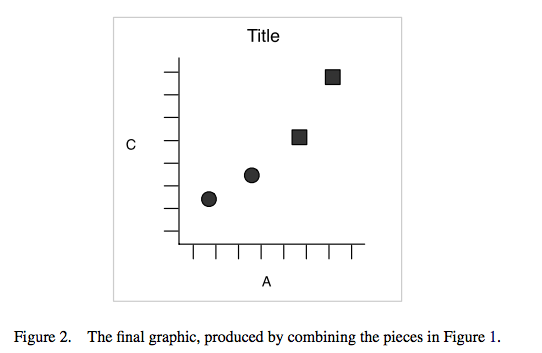
\includegraphics{imgs/combined.png}

Let's have a look at what this looks like for a graph.

Let's have a look at some data about
\href{https://www.gov.uk/government/publications/football-related-arrests-and-banning-orders-england-and-wales-season-2016-to-2017/football-related-arrests-and-banning-order-statistics-england-and-wales-2016-to-2017-season}{banning
orders} for different football clubs.

First you need to read the data. We keep this data in a website and you
can download it with the following code:

\begin{Shaded}
\begin{Highlighting}[]
\NormalTok{fbo_url <-}\StringTok{ "https://raw.githubusercontent.com/maczokni/R-for-Criminologists/master/fbo-by-club-supported-cleaned.csv"}
\NormalTok{fbo <-}\StringTok{ }\KeywordTok{read.csv}\NormalTok{(}\KeywordTok{url}\NormalTok{(fbo_url))}
\end{Highlighting}
\end{Shaded}

Now let's explore the question of number of banning orders for clubs in
different leagues. But as a first step, let's just plot the number of
banning orders for each club. Let's build this plot:

\begin{Shaded}
\begin{Highlighting}[]
\KeywordTok{ggplot}\NormalTok{(}\DataTypeTok{data =}\NormalTok{ fbo, }\KeywordTok{aes}\NormalTok{(}\DataTypeTok{x =}\NormalTok{ Club.Supported, }\DataTypeTok{y=}\NormalTok{Banning.Orders)) }\OperatorTok{+}\StringTok{          }\CommentTok{#data}
\StringTok{   }\KeywordTok{geom_point}\NormalTok{() }\OperatorTok{+}\StringTok{                           }\CommentTok{#geometry}
\StringTok{  }\KeywordTok{theme_bw}\NormalTok{()                                    }\CommentTok{#backgroud coordinate system}
\end{Highlighting}
\end{Shaded}

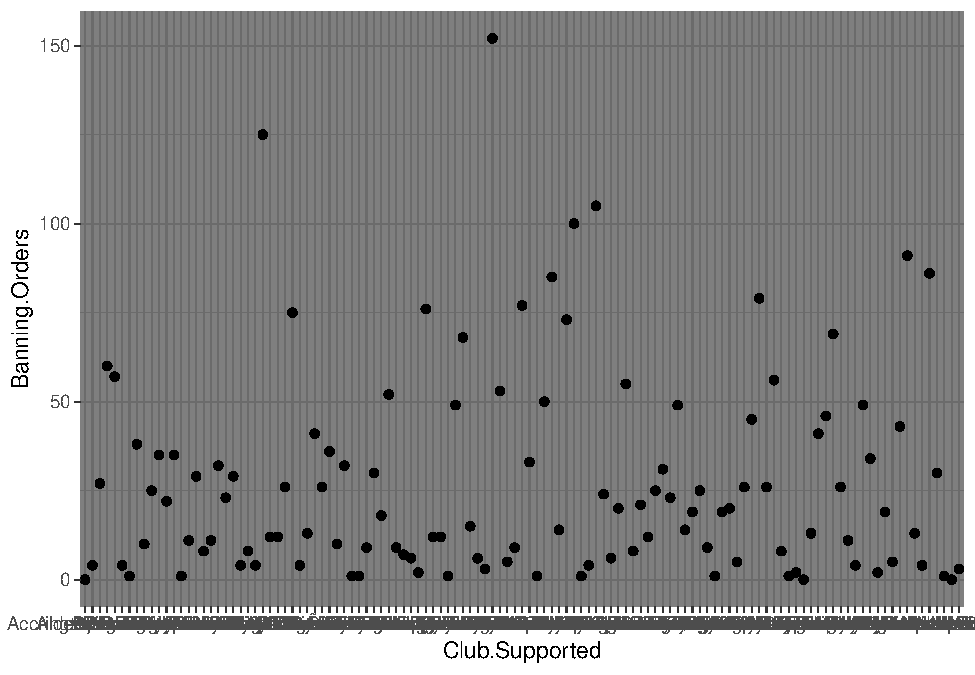
\includegraphics{03-visualisation_files/figure-latex/unnamed-chunk-4-1.pdf}

The first line above begins a plot by calling the \texttt{ggplot()}
function, and putting the data into it. You have to name your dataframe,
and then, within the \texttt{aes()} command you pass the specific
variables which you want to plot. In this case, we only want to see the
distribution of one variable, banning orders, in the y axis and we will
plot the club supported in the x axis.

The second line is where we add the geometry. This is where we tell R
what we want the graph to be. Here we say we want it to be points by
using geom\_points. You can see a list of all possible geoms
\href{http://docs.ggplot2.org/current/}{here}.

The third line is where we can tweak the display of the graph. Here I
used theme\_bw() which is a nice clean theme. You can try with other
themes. To get a list of themes you can also see the resource
\href{http://docs.ggplot2.org/current/}{here}.

\begin{Shaded}
\begin{Highlighting}[]
\KeywordTok{ggplot}\NormalTok{(}\DataTypeTok{data =}\NormalTok{ fbo, }\KeywordTok{aes}\NormalTok{(}\DataTypeTok{x =}\NormalTok{ Club.Supported, }\DataTypeTok{y=}\NormalTok{Banning.Orders)) }\OperatorTok{+}\StringTok{     }\CommentTok{#data}
\StringTok{   }\KeywordTok{geom_point}\NormalTok{() }\OperatorTok{+}\StringTok{                                                   }\CommentTok{#geometry}
\StringTok{  }\KeywordTok{theme_dark}\NormalTok{()                                                      }\CommentTok{#backgroud coordinate system}
\end{Highlighting}
\end{Shaded}

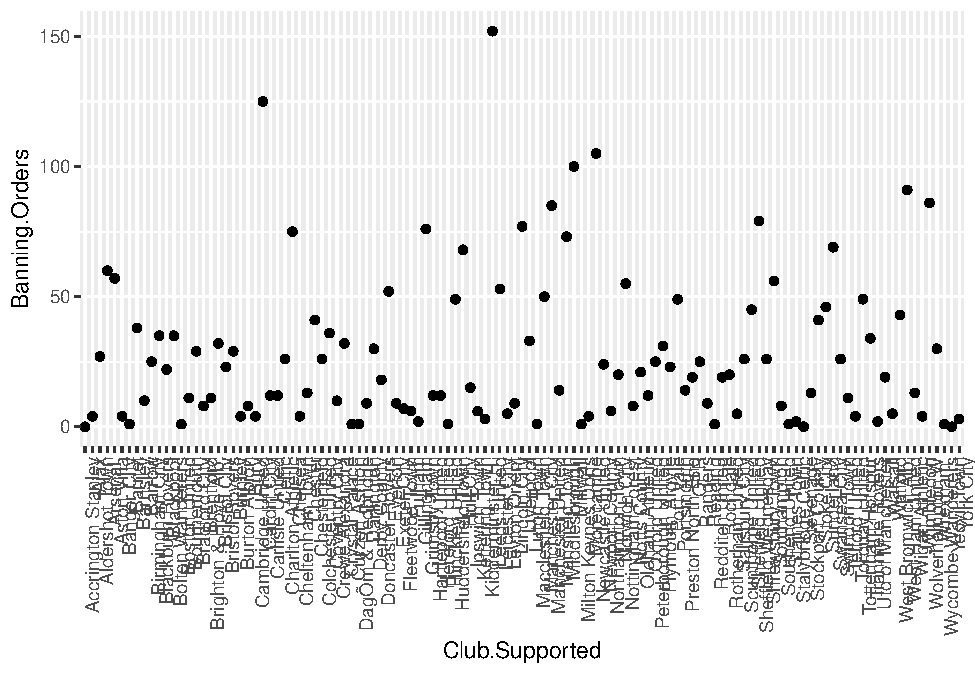
\includegraphics{03-visualisation_files/figure-latex/unnamed-chunk-5-1.pdf}

Changing the theme is not all you can do with the third element. For
example here you can't really read the axis labels, because they're all
overlapping. One solution would be to rotate your axis labels 90
degrees, with the following code:
\texttt{axis.text.x\ =\ element\_text(angle\ =\ 90,\ hjust\ =\ 1)}. You
pass this code to the theme argument.

\begin{Shaded}
\begin{Highlighting}[]
\KeywordTok{ggplot}\NormalTok{(}\DataTypeTok{data =}\NormalTok{ fbo, }\KeywordTok{aes}\NormalTok{(}\DataTypeTok{x =}\NormalTok{ Club.Supported, }\DataTypeTok{y=}\NormalTok{Banning.Orders)) }\OperatorTok{+}\StringTok{     }
\StringTok{   }\KeywordTok{geom_point}\NormalTok{() }\OperatorTok{+}\StringTok{                                                   }
\StringTok{  }\KeywordTok{theme}\NormalTok{(}\DataTypeTok{axis.text.x =} \KeywordTok{element_text}\NormalTok{(}\DataTypeTok{angle =} \DecValTok{90}\NormalTok{, }\DataTypeTok{hjust =} \DecValTok{1}\NormalTok{))                                   }
\end{Highlighting}
\end{Shaded}

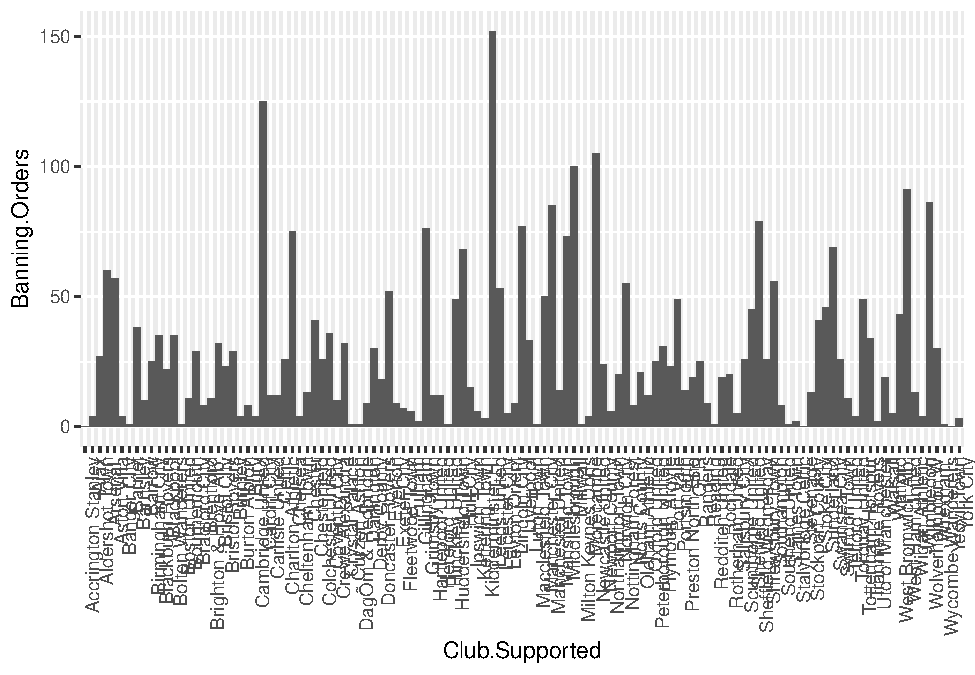
\includegraphics{03-visualisation_files/figure-latex/unnamed-chunk-6-1.pdf}

OK what if we don't want it to be points, but instead we wanted it to be
a bar graph?

\begin{Shaded}
\begin{Highlighting}[]
\KeywordTok{ggplot}\NormalTok{(}\DataTypeTok{data =}\NormalTok{ fbo, }\KeywordTok{aes}\NormalTok{(}\DataTypeTok{x =}\NormalTok{ Club.Supported, }\DataTypeTok{y=}\NormalTok{Banning.Orders)) }\OperatorTok{+}\StringTok{   }\CommentTok{#data}
\StringTok{   }\KeywordTok{geom_bar}\NormalTok{(}\DataTypeTok{stat =} \StringTok{"identity"}\NormalTok{) }\OperatorTok{+}\StringTok{                                  }\CommentTok{#geometry}
\StringTok{  }\KeywordTok{theme}\NormalTok{(}\DataTypeTok{axis.text.x =} \KeywordTok{element_text}\NormalTok{(}\DataTypeTok{angle =} \DecValTok{90}\NormalTok{, }\DataTypeTok{hjust =} \DecValTok{1}\NormalTok{))                                                       }\CommentTok{#backgroud coordinate system}
\end{Highlighting}
\end{Shaded}

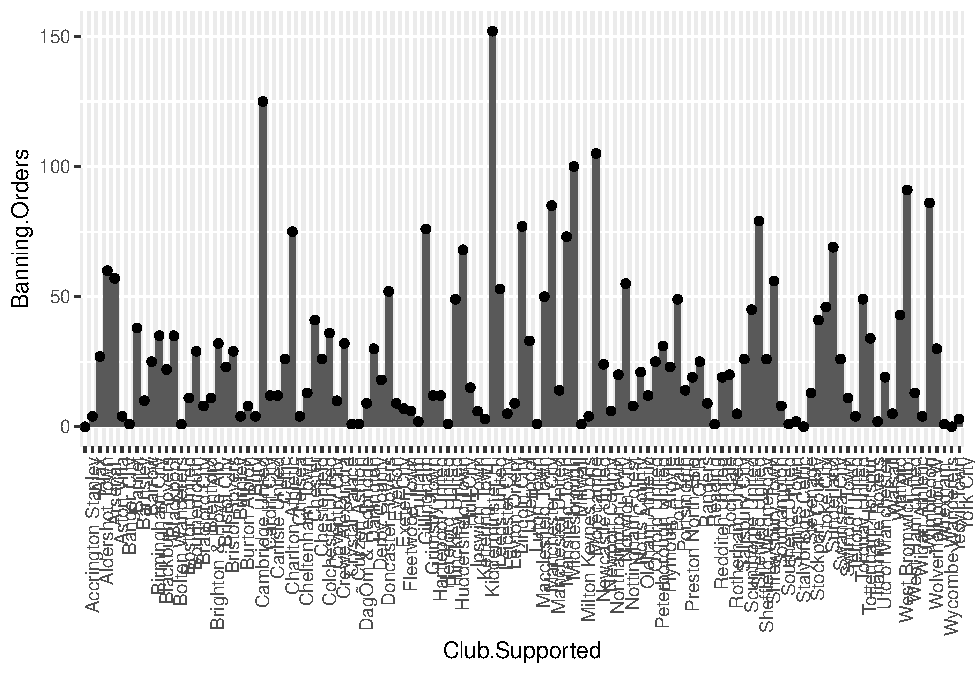
\includegraphics{03-visualisation_files/figure-latex/unnamed-chunk-7-1.pdf}

You might notice here we pass an argument \texttt{stat\ =\ "identity"}
to \texttt{geo\_bar()} function. This is because you can have a bar
graph where the height of the bar shows frequency (stat = ``count''), or
where the height is taken from a variable in your dataframe (stat =
``identity''). Here we specified a y-value (height) as the
Banning.Orders variable.

So this is cool! But what if I like both?

Well this is the beauty of the layering approach of ggplot2. You can
layer on as many geoms as your little heart desires! XD

\begin{Shaded}
\begin{Highlighting}[]
\KeywordTok{ggplot}\NormalTok{(}\DataTypeTok{data =}\NormalTok{ fbo, }\KeywordTok{aes}\NormalTok{(}\DataTypeTok{x =}\NormalTok{ Club.Supported, }\DataTypeTok{y=}\NormalTok{Banning.Orders)) }\OperatorTok{+}\StringTok{  }\CommentTok{#data}
\StringTok{  }\KeywordTok{geom_bar}\NormalTok{(}\DataTypeTok{stat =} \StringTok{"identity"}\NormalTok{) }\OperatorTok{+}\StringTok{                                  }\CommentTok{#geometry 1 }
\StringTok{  }\KeywordTok{geom_point}\NormalTok{()}\OperatorTok{+}\StringTok{                                                  }\CommentTok{#geometry 2}
\KeywordTok{theme}\NormalTok{(}\DataTypeTok{axis.text.x =} \KeywordTok{element_text}\NormalTok{(}\DataTypeTok{angle =} \DecValTok{90}\NormalTok{, }\DataTypeTok{hjust =} \DecValTok{1}\NormalTok{))                                                      }\CommentTok{#backgroud coordinate system}
\end{Highlighting}
\end{Shaded}

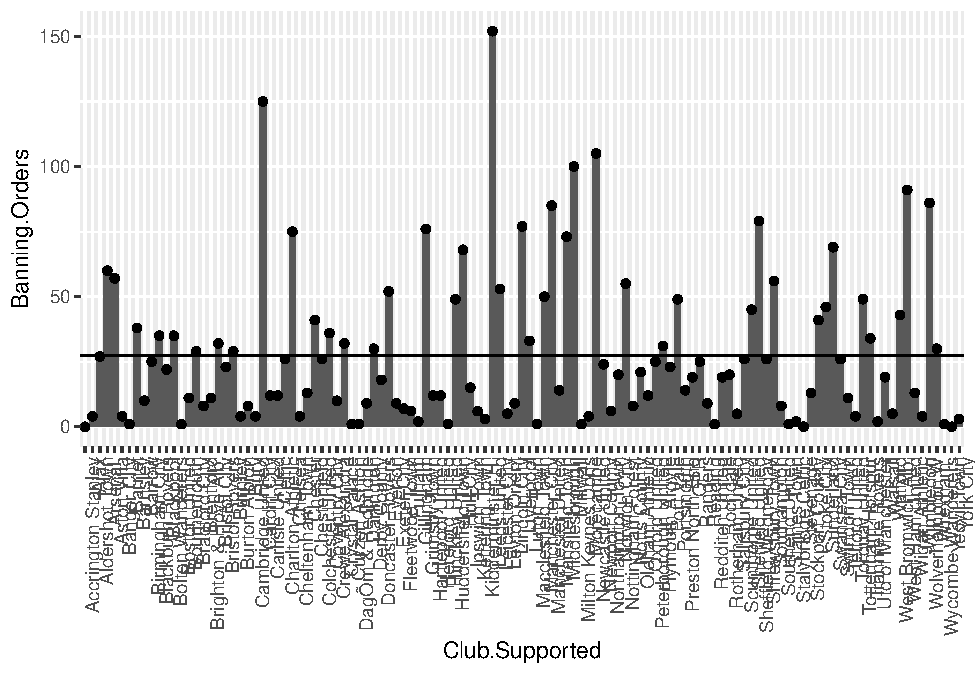
\includegraphics{03-visualisation_files/figure-latex/unnamed-chunk-8-1.pdf}

You can add other things too. For example you can add the mean number of
Banning.Orders:

\begin{Shaded}
\begin{Highlighting}[]
\KeywordTok{ggplot}\NormalTok{(}\DataTypeTok{data =}\NormalTok{ fbo, }\KeywordTok{aes}\NormalTok{(}\DataTypeTok{x =}\NormalTok{ Club.Supported, }\DataTypeTok{y=}\NormalTok{Banning.Orders)) }\OperatorTok{+}\StringTok{  }\CommentTok{#data}
\StringTok{  }\KeywordTok{geom_bar}\NormalTok{(}\DataTypeTok{stat =} \StringTok{"identity"}\NormalTok{) }\OperatorTok{+}\StringTok{                                  }\CommentTok{#geometry 1 }
\StringTok{  }\KeywordTok{geom_point}\NormalTok{() }\OperatorTok{+}\StringTok{                                                 }\CommentTok{#geometry 2}
\StringTok{  }\KeywordTok{geom_hline}\NormalTok{(}\DataTypeTok{yintercept =} \KeywordTok{mean}\NormalTok{(fbo}\OperatorTok{$}\NormalTok{Banning.Orders)) }\OperatorTok{+}\StringTok{            }\CommentTok{#mean line}
\KeywordTok{theme}\NormalTok{(}\DataTypeTok{axis.text.x =} \KeywordTok{element_text}\NormalTok{(}\DataTypeTok{angle =} \DecValTok{90}\NormalTok{, }\DataTypeTok{hjust =} \DecValTok{1}\NormalTok{))                                                      }\CommentTok{#backgroud coordinate system}
\end{Highlighting}
\end{Shaded}

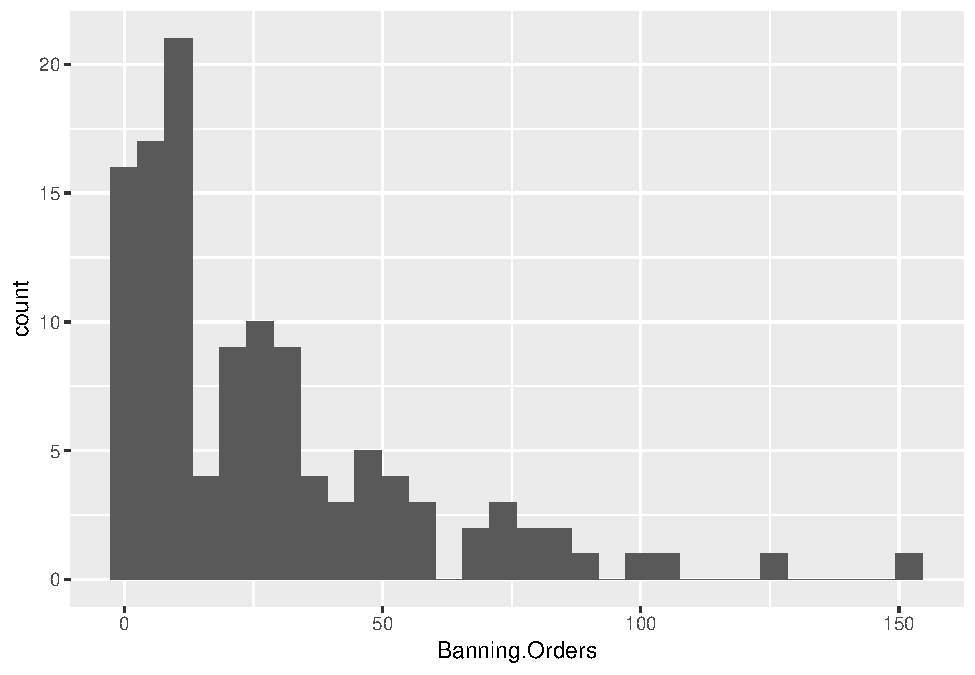
\includegraphics{03-visualisation_files/figure-latex/unnamed-chunk-9-1.pdf}

This is basically all you need to know to build a graph! So far we have
introduced a lot of code some of which you may not fully understand.
Don't worry too much, we just wanted to give you a quick introduction to
some of the possibilities. Later in the session we will go back to some
of these functions in a slower way.

\#\#What graph should I use?

There are a lot of points to consider when you are choosing what graph
to use to visually represent your data. There are some best practice
guidelines, but at the end of the day, you need to consider what is best
for your data. What do you want to show? What graph will best
communicate your message? Is it a comparison between groups? Is it the
frequency distribution of 1 variable?

As some guidance, you can use the below
\href{https://flowingdata.com/2009/01/15/flow-chart-shows-you-what-chart-to-use/}{cheatsheet,
taken from Nathan Yau's blog Flowingdata}:

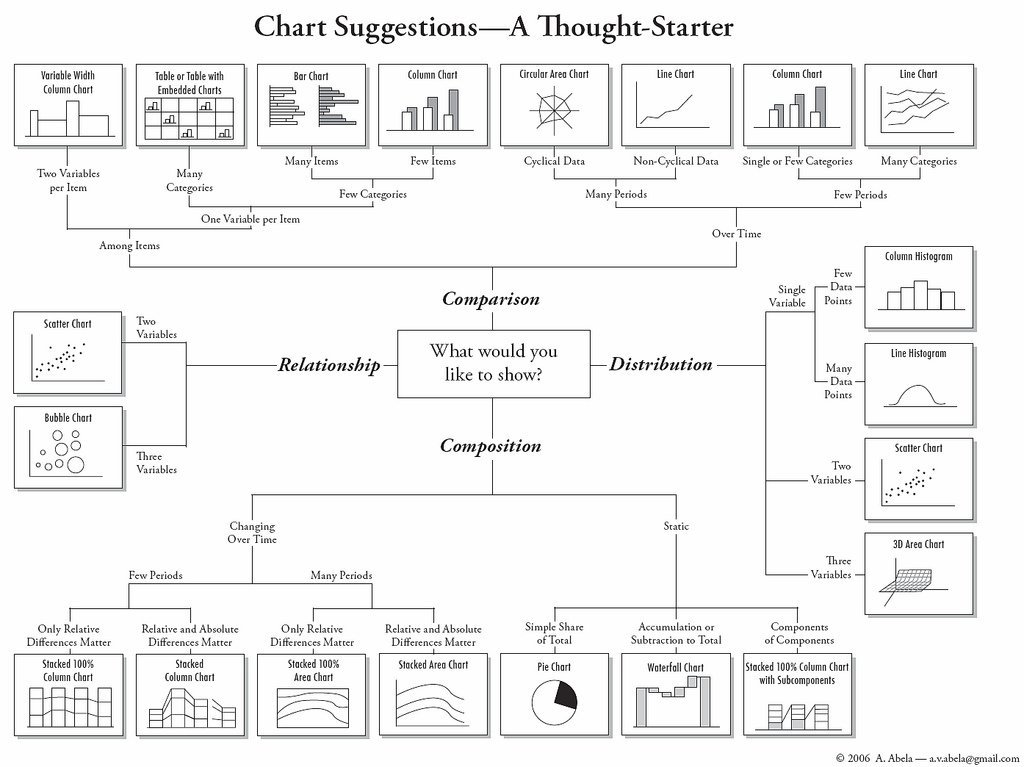
\includegraphics{imgs/chart-chart.jpg}

However, keep in mind that this is more of a guideline, aimed to nudge
you in the right direction. There are many ways to visualise the same
data, and sometimes you might want to experiment with some of these, see
what the differences are.

There is also a vast amount of research into what works in displaying
quantitative information. The classic book is by Edward Tufte \footnote{Various
  of these can be obtained invoking the \texttt{pR2()} function from the
  \texttt{pscl} package.}, but since him there are many other
researchers as well who focus on approaches to displaying data. Two
useful books you may want to consider are Few (2012) \footnote{Alternatively
  one could use the \texttt{ROCR} package. For details, see
  \href{http://rocr.bioinf.mpi-sb.mpg.de/}{here}.} and Cairo (2016)
\footnote{\href{http://blog.minitab.com/blog/adventures-in-statistics/regression-analysis-how-do-i-interpret-r-squared-and-assess-the-goodness-of-fit}{This}
  is a reasonable explanation of how to interpret R-Squared.}. Claus
Wilke is also producing a textbook that is work in progress but freely
available \href{https://serialmentor.com/dataviz/}{in the internet}.
These authors tend to produce recommendations on what to use (and not
use) in certain contexts.

For example, most data visualisation experts agree that you should not
use 3D graphics unless there is a meaning to the third dimension. So
using 3D graphics just for decoration, as in
\href{https://mir-s3-cdn-cf.behance.net/project_modules/disp/2505dd10837923.56030acd2ef20.jpg}{this
case} is normally frowned upon. However there are cases when including a
third dimension is vital to communicating your findings. See this
\href{http://www.visualisingdata.com/2015/03/when-3d-works/}{example}.

Also often certain chart types are villanified. For example, the pie
chart is one such example. A lot of people really dislike pie charts, eg
see
\href{http://www.storytellingwithdata.com/blog/2011/07/death-to-pie-charts}{here}
or
\href{http://www.businessinsider.com/pie-charts-are-the-worst-2013-6?IR=T}{here}.
If you want to display proportion, research indicates that a square pie
chart is more likely to be interpreted correctly by viewers see
\href{https://eagereyes.org/blog/2016/a-reanalysis-of-a-study-about-square-pie-charts-from-2009}{here}

Also, in some cases bar plots can hide important features of your data,
and might not be the most appropriate means for comparison:

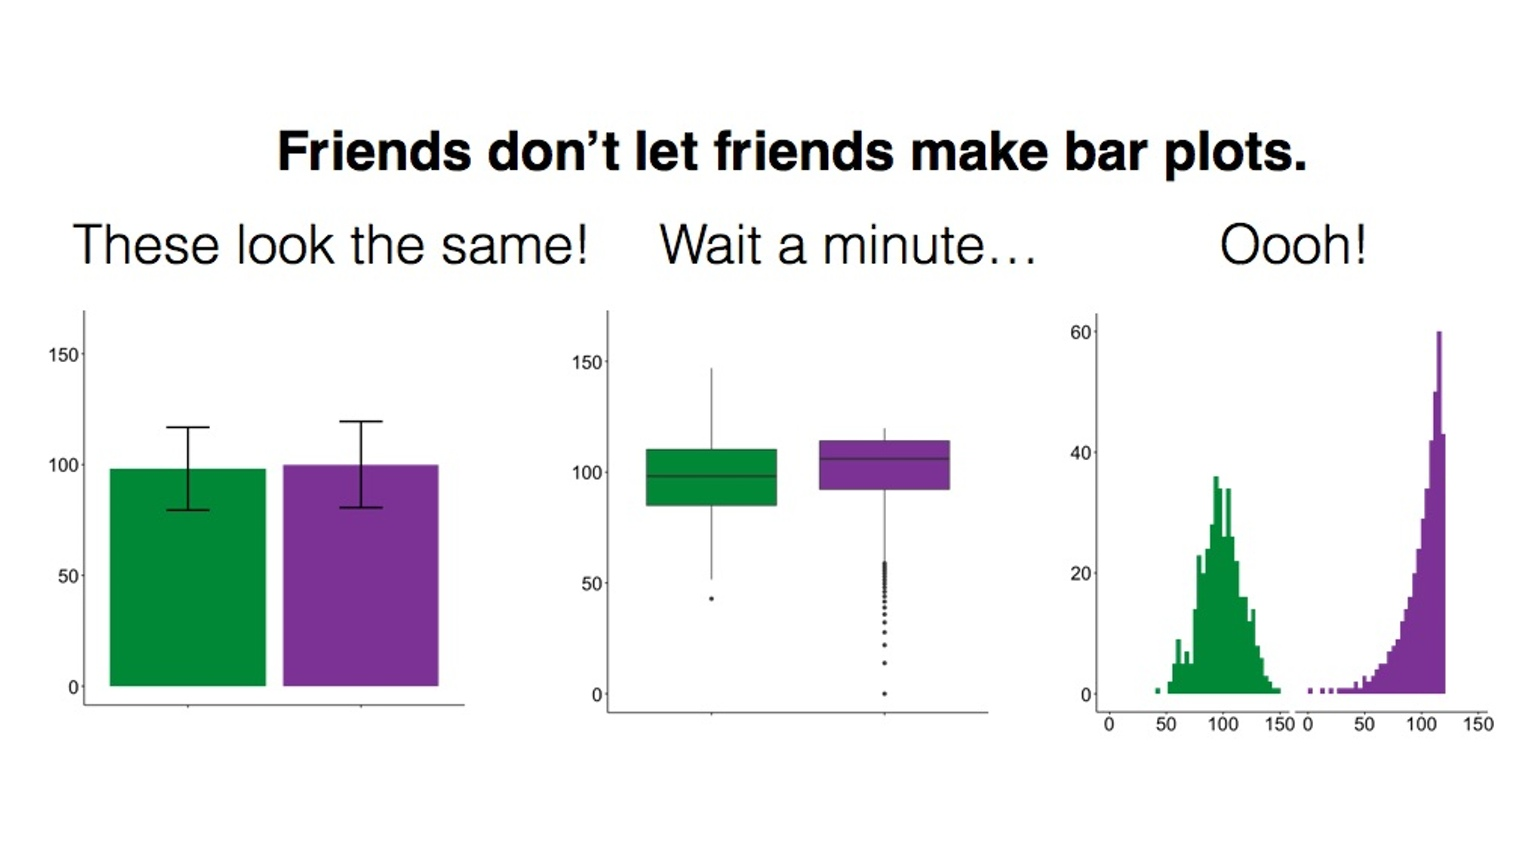
\includegraphics{imgs/barbarplots.jpg}

This has lead to a
\href{https://www.kickstarter.com/projects/1474588473/barbarplots/description}{kickstarter
campaign} around actually banning bar plots\ldots{}!

So choosing the right plot and how to design the different elements of a
plot is somehow of an art that requires practice and a good
understanding of the data visualisation literature. Here we can only
provide you with an introduction to some of these issues. Other books
that focus on

An important consideration is that the plot that you use depends on the
data you are plotting, as well as the message you want to convey with
the plot, the audience that is intended for, and even the format in
which it will be presented (a website, a printed report, a power point
presentation, etc.). So for example, returning again to the difference
between number of banning orders between clubs in different leagues,
what are some ways of plotting these?

One suggestion is to make a histogram for each one. You can use ggplot's
facet\_wrap() option to split graphs by a grouping variable. For
example, to create a histogram of banning orders you write:

\begin{Shaded}
\begin{Highlighting}[]
\KeywordTok{ggplot}\NormalTok{(}\DataTypeTok{data =}\NormalTok{ fbo, }\KeywordTok{aes}\NormalTok{(}\DataTypeTok{x =}\NormalTok{ Banning.Orders)) }\OperatorTok{+}\StringTok{ }
\StringTok{  }\KeywordTok{geom_histogram}\NormalTok{()}
\end{Highlighting}
\end{Shaded}

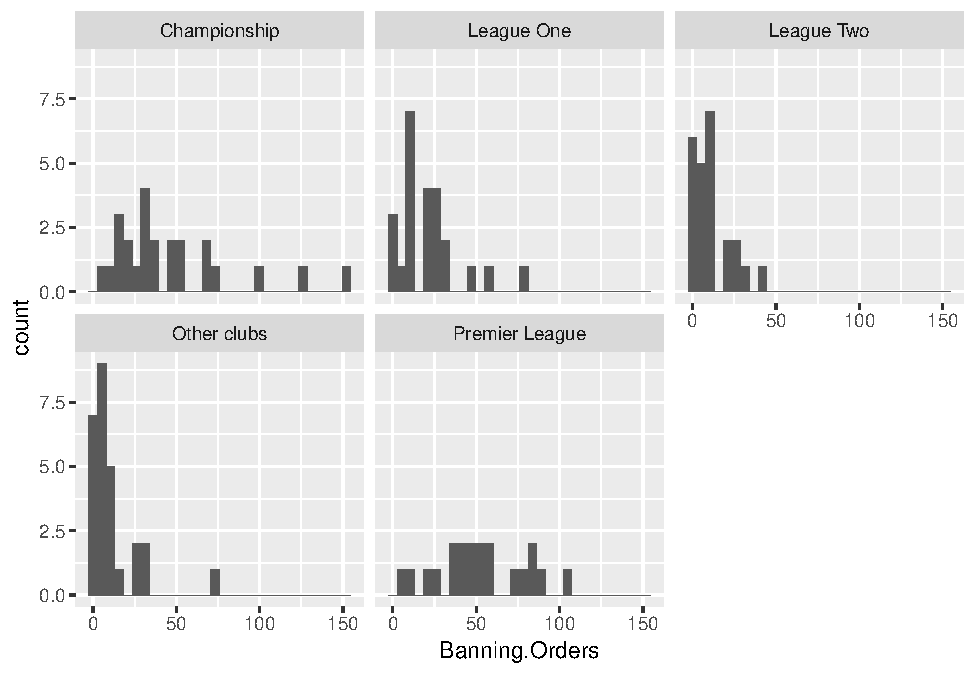
\includegraphics{03-visualisation_files/figure-latex/unnamed-chunk-10-1.pdf}

Now to split this by League.of.the.Club.Supported, you use facet\_wrap()
in the coordinate layer of the plot.

\begin{Shaded}
\begin{Highlighting}[]
\KeywordTok{ggplot}\NormalTok{(}\DataTypeTok{data =}\NormalTok{ fbo, }\KeywordTok{aes}\NormalTok{(}\DataTypeTok{x =}\NormalTok{ Banning.Orders)) }\OperatorTok{+}\StringTok{ }
\StringTok{  }\KeywordTok{geom_histogram}\NormalTok{() }\OperatorTok{+}\StringTok{ }
\StringTok{  }\KeywordTok{facet_wrap}\NormalTok{(}\OperatorTok{~}\NormalTok{League.of.the.Club.Supported)}
\end{Highlighting}
\end{Shaded}

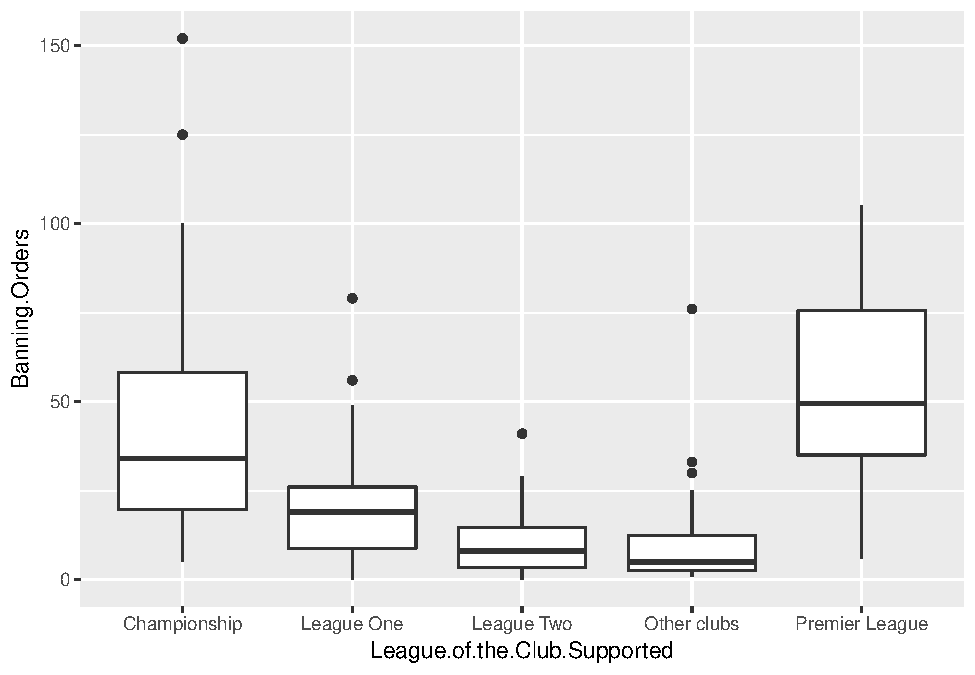
\includegraphics{03-visualisation_files/figure-latex/unnamed-chunk-11-1.pdf}

Well you can see there's different distribution in each league. But is
this easy to compare? Maybe another approach would make it easier?
Personally I like boxplots for showing distribution. So let's try:

\begin{Shaded}
\begin{Highlighting}[]
\KeywordTok{ggplot}\NormalTok{(}\DataTypeTok{data =}\NormalTok{ fbo, }\KeywordTok{aes}\NormalTok{(}\DataTypeTok{x =}\NormalTok{ League.of.the.Club.Supported, }\DataTypeTok{y =}\NormalTok{ Banning.Orders)) }\OperatorTok{+}\StringTok{ }
\StringTok{  }\KeywordTok{geom_boxplot}\NormalTok{() }
\end{Highlighting}
\end{Shaded}

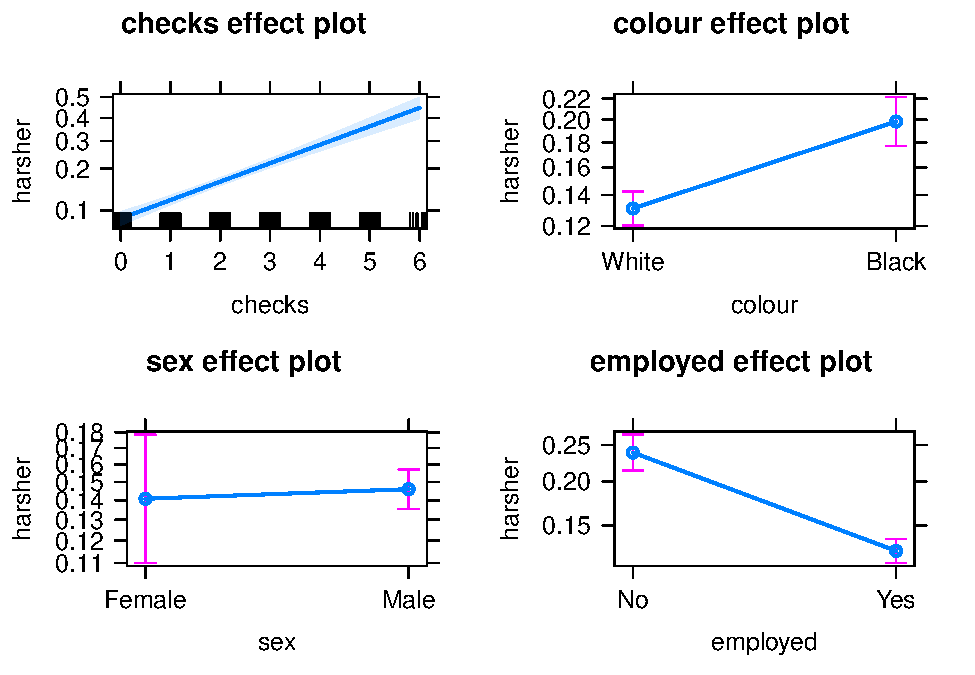
\includegraphics{03-visualisation_files/figure-latex/unnamed-chunk-12-1.pdf}

This makes the comparison significantly easier, right? But the order is
strange! Remember we talked about factors in previous weeks? Well the
good thing about factors is that we can arrange them in their natural
order. If we dont' describe an order, then R uses the alphabetical
order. So let's reorder our factor. To do that we are specifying the
levels in the order in which we want to be embedded witin the factor. We
use code we introduced last week to do this.

\begin{Shaded}
\begin{Highlighting}[]
\NormalTok{fbo}\OperatorTok{$}\NormalTok{League.of.the.Club.Supported <-}\StringTok{ }\KeywordTok{factor}\NormalTok{(fbo}\OperatorTok{$}\NormalTok{League.of.the.Club.Supported, }\DataTypeTok{levels =} \KeywordTok{c}\NormalTok{(}\StringTok{"Premier League"}\NormalTok{, }\StringTok{"Championship"}\NormalTok{, }\StringTok{"League One"}\NormalTok{, }\StringTok{"League Two"}\NormalTok{, }\StringTok{"Other clubs"}\NormalTok{))}
\end{Highlighting}
\end{Shaded}

And now create the plot again!

\begin{Shaded}
\begin{Highlighting}[]
\KeywordTok{ggplot}\NormalTok{(}\DataTypeTok{data =}\NormalTok{ fbo, }\KeywordTok{aes}\NormalTok{(}\DataTypeTok{x =}\NormalTok{ League.of.the.Club.Supported, }\DataTypeTok{y =}\NormalTok{ Banning.Orders)) }\OperatorTok{+}\StringTok{ }
\StringTok{  }\KeywordTok{geom_boxplot}\NormalTok{() }
\end{Highlighting}
\end{Shaded}

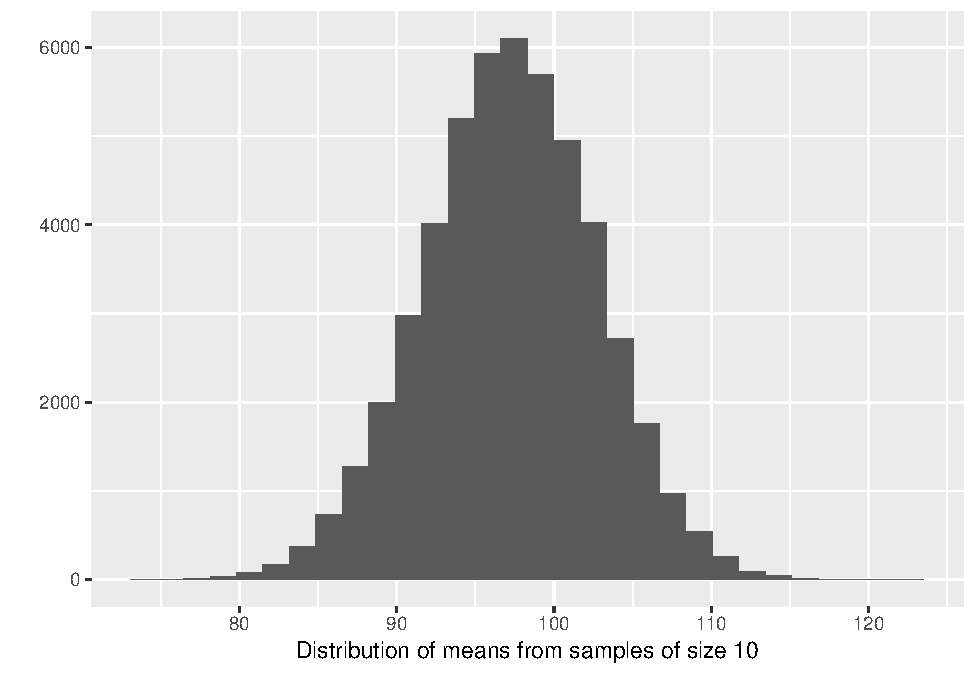
\includegraphics{03-visualisation_files/figure-latex/unnamed-chunk-14-1.pdf}

Now this is great! We can see that the higher the league the more
banning orders they have. Any ideas why?

We'll now go through some examples of making graphs using ggplot package
stopping a bit more on each of them.

\#\#Histograms

\href{http://www.learner.org/courses/againstallodds/unitpages/unit03.html}{Histograms}
are useful ways of representing quantitative variables visually.

As mentioned earlier, we will emphasise in this course the use of the
\texttt{ggplot()} function. With \texttt{ggplot()} you start with a
blank canvass and keep adding specific layers. The \texttt{ggplot()}
function can specify the dataset and the aesthetics (the visual
characteristics that represent the data).

To get the data we're going to use here, load up the package ``MASS''
and then call the Boston data into your environment.

\begin{Shaded}
\begin{Highlighting}[]
\KeywordTok{library}\NormalTok{(MASS)}
\KeywordTok{data}\NormalTok{(Boston)}
\end{Highlighting}
\end{Shaded}

This package has a dataframe called ``Boston''. This has data about
Housing Values in suburbs of Boston (USA). To access the codebook (how
you find out what variables are) use the ``?''.

OK so let's make a graph about the variable which represents the per
capita crime rate by town ('crim').

If you want to produce a histogram with the \texttt{ggplot} function you
would use the following equivalent code:

\begin{Shaded}
\begin{Highlighting}[]
\KeywordTok{ggplot}\NormalTok{(Boston, }\KeywordTok{aes}\NormalTok{(}\DataTypeTok{x =}\NormalTok{ crim)) }\OperatorTok{+}\StringTok{ }
\StringTok{  }\KeywordTok{geom_histogram}\NormalTok{()}
\end{Highlighting}
\end{Shaded}

\begin{verbatim}
## `stat_bin()` using `bins = 30`. Pick better value with `binwidth`.
\end{verbatim}

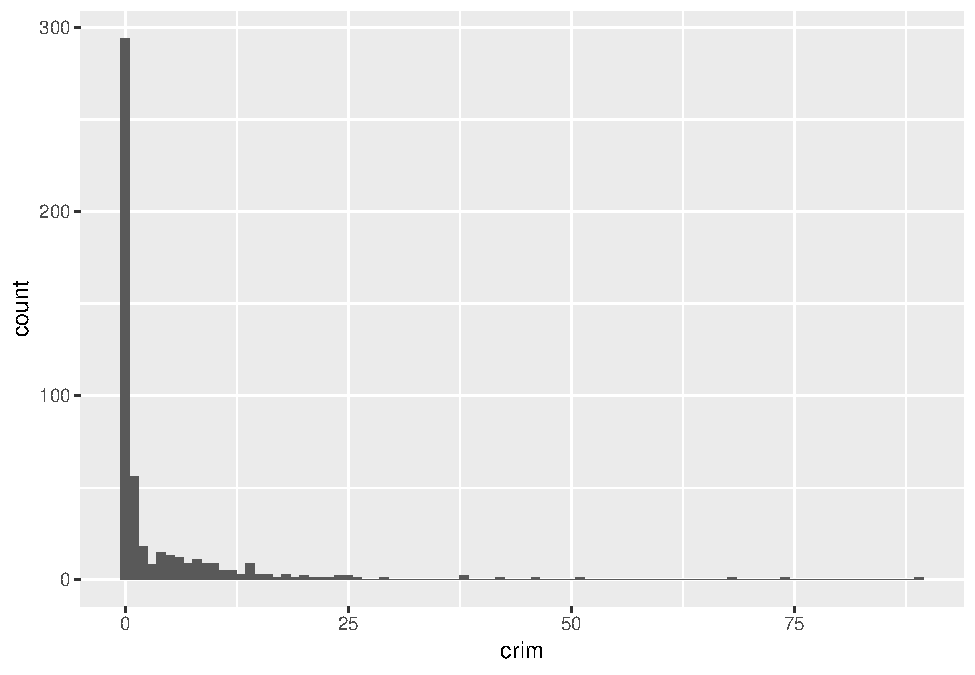
\includegraphics{03-visualisation_files/figure-latex/unnamed-chunk-16-1.pdf}

So you can see that \texttt{ggplot} works in a way that you can add a
series of additional specifications (layers, annotations). In this
simple plot the \texttt{ggplot} function simply maps \emph{crim} as the
variable to be displayed (as one of the aesthetics) and the dataset.
Then you add the \texttt{geom\_histogram} to tell R that you want this
variable to be represented as a histogram. Later we will see what other
things you can add.

A histogram is simply putting cases in ``bins'' and then creates a bar
for each bin. You can think of it as a visual grouped frequency
distribution. The code we have used so far has used a bin-width of size
range/30 as R kindly reminded us in the output. But you can modify this
parameter if you want to get a rougher or a more granular picture. In
fact, you should \emph{always} play around with different specifications
of the bin-width until you find one that tells the full story in a
parsimonious way.

\begin{Shaded}
\begin{Highlighting}[]
\KeywordTok{ggplot}\NormalTok{(Boston, }\KeywordTok{aes}\NormalTok{(}\DataTypeTok{x =}\NormalTok{ crim)) }\OperatorTok{+}
\StringTok{  }\KeywordTok{geom_histogram}\NormalTok{(}\DataTypeTok{binwidth =} \DecValTok{1}\NormalTok{) }
\end{Highlighting}
\end{Shaded}

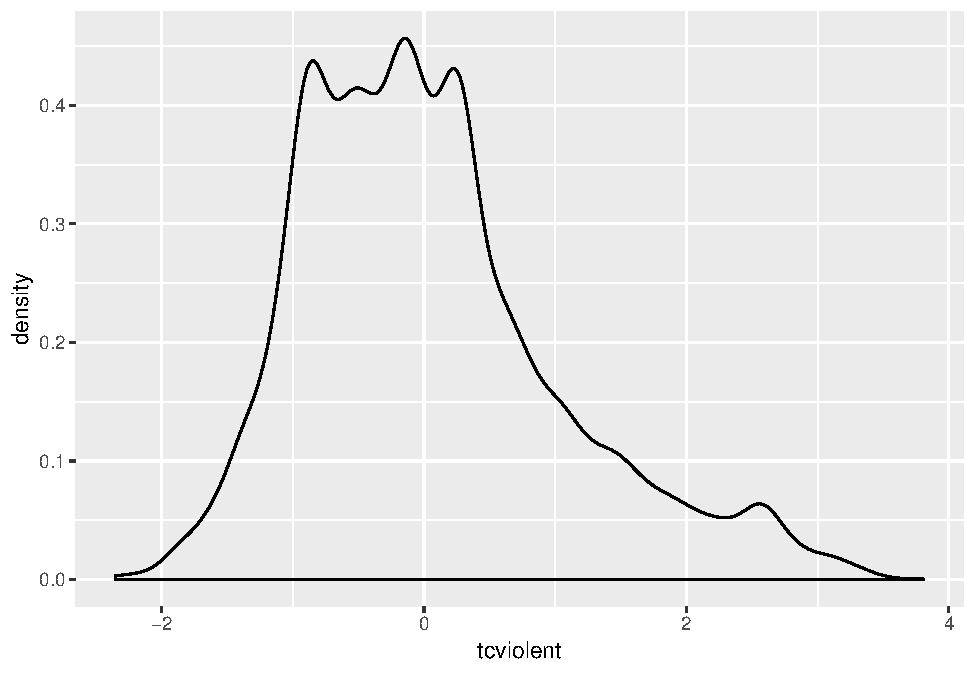
\includegraphics{03-visualisation_files/figure-latex/unnamed-chunk-17-1.pdf}

We can pass arguments to the the geoms, here we are changing the size of
the bins (for further details on other arguments you can check the help
files). Using bin-width of 1 we are essentially creating a bar for every
one unit increase in the percent rate of crime. We can still see that
most towns have a very low level of crime.

Let's sum the number of towns with a value lower than 1 in the per
capita crime rate. We use the sum function for this, specifying we are
only interested in adding cases where the value of the variable crim is
lower than 1.

\begin{Shaded}
\begin{Highlighting}[]
\KeywordTok{sum}\NormalTok{(Boston}\OperatorTok{$}\NormalTok{crim }\OperatorTok{<}\StringTok{ }\DecValTok{1}\NormalTok{)}
\end{Highlighting}
\end{Shaded}

\begin{verbatim}
## [1] 332
\end{verbatim}

We can see that the large majority of towns, 332 out of 506, have a per
capita crime rate below 1\%. But we can also see that there are some
towns that have a high concentration of crime. This is a spatial feature
of crime; it tends to concentrate in particular areas and places. You
can see how we can use visualisations to show the data and get a first
feeling for how it may be distributed.

When plotting a continuous variable we are interested in the following
features:

\begin{itemize}
\tightlist
\item
  \textbf{Asymmetry}: whether the distribution is skewed to the right or
  to the left.
\item
  \textbf{Outliers}: Are there one or more values that seem very unlike
  the others?
\item
  \textbf{Multimodality}: How many peaks has the distribution? More than
  one peak may indicate that the variable is measuring different groups.
\item
  \textbf{Impossibilities or other anomalies}: Values that are simply
  unrealistic given what we are measuring (e.g., somebody with an age of
  a 1000 years). Sometimes you may come across a distribution of data
  with a very high (and implausible) frequency count for a particular
  value. Maybe you measure age and you have a large number of cases aged
  99 (which is often a code used for missing data).
\item
  \textbf{Spread}: this gives us an idea of variability in our data.
\end{itemize}

Often we visualise data because we want to compare distributions.
\textbf{Most of data analysis is about making comparisons}. We are going
to explore whether the distribution of crime in this dataset is
different for less affluent areas. The variable \emph{medv} measures in
the Boston dataset the median value of owner-occupied homes. For the
purposes of this illustration I want to dichotomise\footnote{\href{http://www.sumsar.net/blog/2013/12/an-animation-of-the-construction-of-a-confidence-interval/}{This
  blog post} provides a nice animation of the confidence interval and
  hypothesis testing.} this variable, to create a group of towns with
particularly low values versus all the others. For further details in
how to recode variables with R you may want to read the relevant
sections in
\href{http://www.statmethods.net/management/variables.html}{Quick R} or
the \href{http://www.cookbook-r.com/Manipulating_data/Recoding_data/}{R
Cookbook}. We will learn more about recoding and transforming variables
in R soon.

How can we create a categorical variable based on information from a
quantitative variable? Let's see the following code and pay attention to
it and the explanation below.

\begin{Shaded}
\begin{Highlighting}[]
\NormalTok{Boston}\OperatorTok{$}\NormalTok{lowval[Boston}\OperatorTok{$}\NormalTok{medv }\OperatorTok{<=}\StringTok{ }\FloatTok{17.02}\NormalTok{] <-}\StringTok{ "Low value"} 
\NormalTok{Boston}\OperatorTok{$}\NormalTok{lowval[Boston}\OperatorTok{$}\NormalTok{medv }\OperatorTok{>}\StringTok{ }\FloatTok{17.02}\NormalTok{] <-}\StringTok{ "Higher value"}
\end{Highlighting}
\end{Shaded}

First we tell R to create a new vector (``lowval'') in the Boston data
frame. This vector will be assigned the character value ``Low value''
when the condition within the square brackets is met. That is, we are
saying that whenever the value in ``medv'' is below 17.02 then the new
variable lowval will equal ``Low value''. I have chosen 17.02 as this is
the first quartile for medv. Then we tell R that when the value is
greater than 17.02 we will assign those cases to a new textual category
called ``Higher Value''.

The variable we created was a character vector (as we can see if we run
the class function). so we are going to transform it into a factor using
the as.factor function (many functions designed to work with categorical
variables expect a factor as an input, not just a character vector). If
we rerun the class function we will see we changed the original variable

\begin{Shaded}
\begin{Highlighting}[]
\KeywordTok{class}\NormalTok{(Boston}\OperatorTok{$}\NormalTok{lowval)}
\end{Highlighting}
\end{Shaded}

\begin{verbatim}
## [1] "character"
\end{verbatim}

\begin{Shaded}
\begin{Highlighting}[]
\NormalTok{Boston}\OperatorTok{$}\NormalTok{lowval <-}\StringTok{ }\KeywordTok{as.factor}\NormalTok{(Boston}\OperatorTok{$}\NormalTok{lowval)}
\KeywordTok{class}\NormalTok{(Boston}\OperatorTok{$}\NormalTok{lowval)}
\end{Highlighting}
\end{Shaded}

\begin{verbatim}
## [1] "factor"
\end{verbatim}

Now we can produce the plot. We will do this using facets. Facets are
another element of the grammar of graphics, we use it to define subsets
of the data to be represented as multiple groups, here we are asking R
to produce two plots defined by the two levels of the factor we just
created.

\begin{Shaded}
\begin{Highlighting}[]
\KeywordTok{ggplot}\NormalTok{(Boston, }\KeywordTok{aes}\NormalTok{(}\DataTypeTok{x =}\NormalTok{ crim)) }\OperatorTok{+}
\StringTok{  }\KeywordTok{geom_histogram}\NormalTok{(}\DataTypeTok{binwidth =} \DecValTok{1}\NormalTok{) }\OperatorTok{+}
\StringTok{  }\KeywordTok{facet_grid}\NormalTok{(lowval }\OperatorTok{~}\StringTok{ }\NormalTok{.) }
\end{Highlighting}
\end{Shaded}

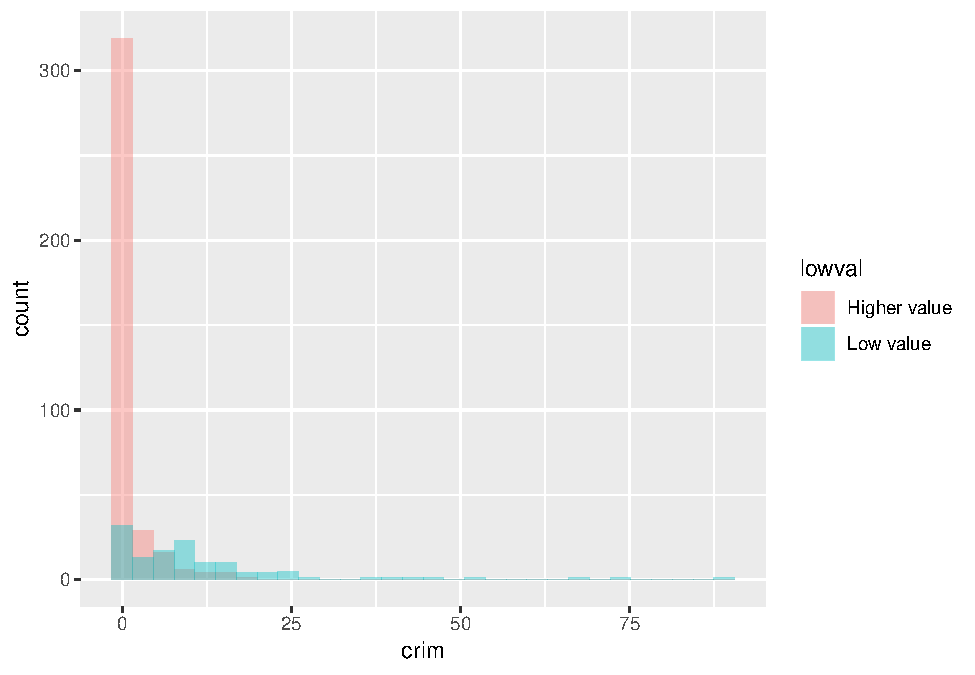
\includegraphics{03-visualisation_files/figure-latex/unnamed-chunk-21-1.pdf}

Visually this may not look great, but it begins to tell a story. We can
see that there is a considerable lower proportion of towns with low
levels of crime in the group of towns that have cheaper homes. It is a
flatter, less skewed distribution. You can see how the
\texttt{facet\_grid()} expression is telling R to create the histogram
of the variable mentioned in the ggplot function for the groups defined
by the categorical input of interest (the factor ``lowval'').

Instead of using facets, we could overlay the histograms with a bit of
transparency. Transparencies work better in screens than in printed
document, so keep in mind this when deciding whether to use them instead
of facets. The code is as follows:

\begin{Shaded}
\begin{Highlighting}[]
\KeywordTok{ggplot}\NormalTok{(Boston, }\KeywordTok{aes}\NormalTok{(}\DataTypeTok{x =}\NormalTok{ crim, }\DataTypeTok{fill =}\NormalTok{ lowval)) }\OperatorTok{+}\StringTok{ }
\StringTok{  }\KeywordTok{geom_histogram}\NormalTok{(}\DataTypeTok{position =} \StringTok{"identity"}\NormalTok{, }\DataTypeTok{alpha =} \FloatTok{0.4}\NormalTok{)}
\end{Highlighting}
\end{Shaded}

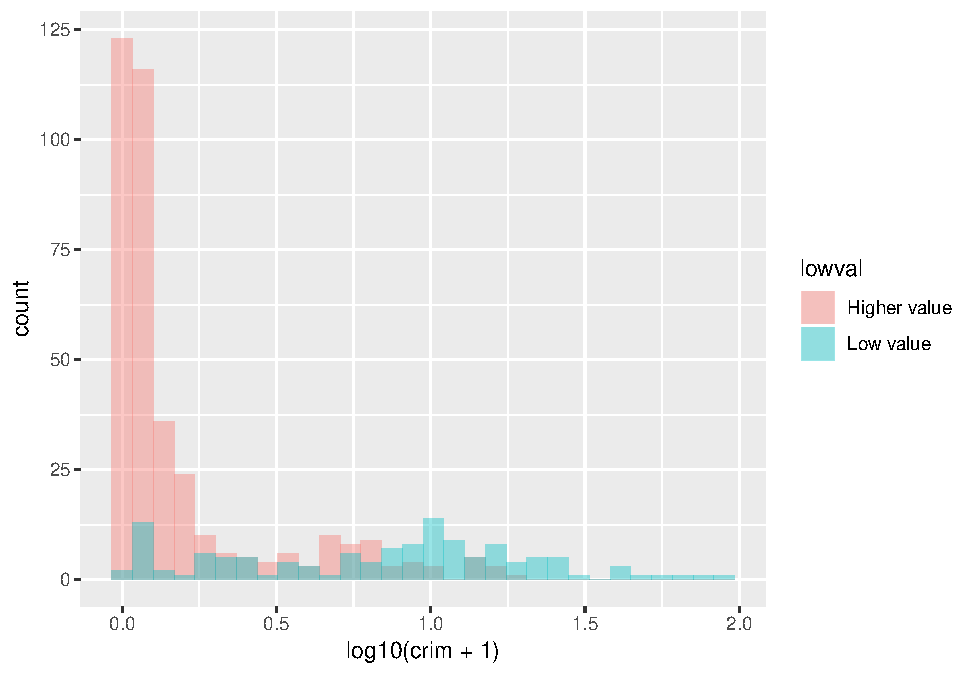
\includegraphics{03-visualisation_files/figure-latex/unnamed-chunk-22-1.pdf}

In the code above, the \texttt{fill} argument identifies the factor
variable in the dataset grouping the cases. Also,
\texttt{position\ =\ identity} tells R to overlay the distributions and
\texttt{alpha} asks for the degree of transparency, a lower value (e.g.,
0.2) will be more transparent.

In this case, part of the problem we have is that the skew can make it
difficult to appreciate the differences. When you are dealing with
skewed distributions such as this, it is sometimes convenient to use a
transformation \footnote{\href{http://vudlab.com/simpsons/}{This} is a
  nice illustration of the Simpon's Paradox, a well known example of
  ommitted variable bias.}. We will come back to this later this
semester. For now suffice to say, that taking the logarithm of a skewed
variable helps to reduce the skew and to see patterns more clearly. In
order to visualise the differences here a bit better we could ask for
the logarithm of the crime per capita rate. Notice how I also add a
constant of 1 to the variable \emph{crim}, this is to avoid NA values in
the newly created variable if the value in \emph{crim} is zero (you
cannot take the log of 0).

\begin{Shaded}
\begin{Highlighting}[]
\KeywordTok{ggplot}\NormalTok{(Boston, }\KeywordTok{aes}\NormalTok{(}\DataTypeTok{x =} \KeywordTok{log10}\NormalTok{(crim }\OperatorTok{+}\StringTok{ }\DecValTok{1}\NormalTok{), }\DataTypeTok{fill =}\NormalTok{ lowval)) }\OperatorTok{+}
\StringTok{  }\KeywordTok{geom_histogram}\NormalTok{(}\DataTypeTok{position =} \StringTok{"identity"}\NormalTok{, }\DataTypeTok{alpha =} \FloatTok{0.4}\NormalTok{)}
\end{Highlighting}
\end{Shaded}

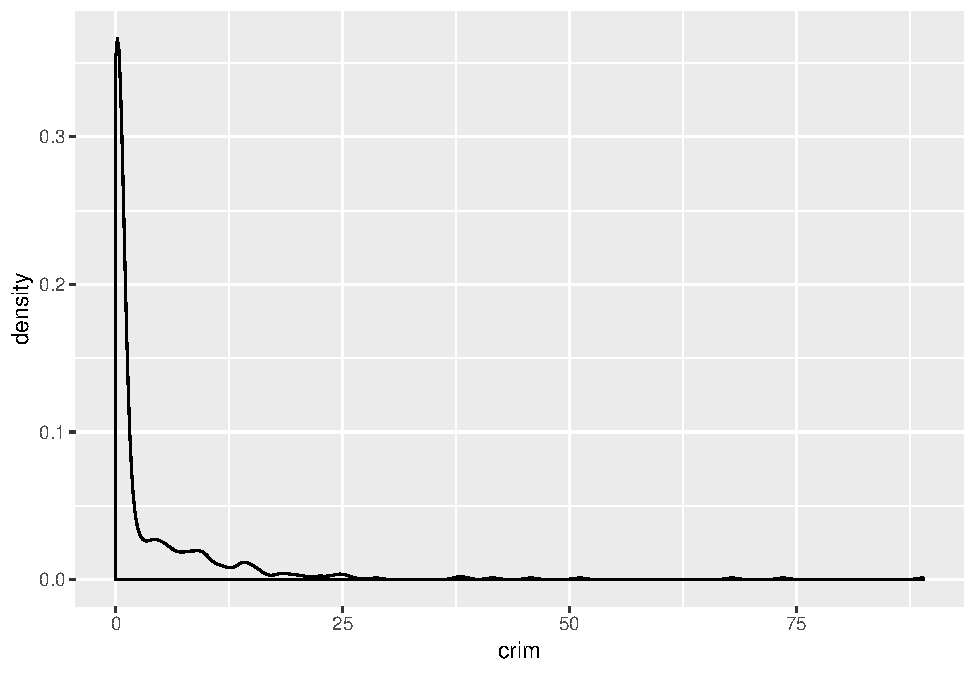
\includegraphics{03-visualisation_files/figure-latex/unnamed-chunk-23-1.pdf}

The plot now is a bit clearer. It seems pretty evident that the
distribution of crime is slightly different between these two types of
towns.

\#\#Density plots

For smoother distributions, you can use density plot. You should have a
healthy amount of data to use these or you could end up with a lot of
unwanted noise. Let's first look at the single density plot for all
cases. Notice all we are doing is invoking a different kind of geom:

\begin{Shaded}
\begin{Highlighting}[]
\KeywordTok{ggplot}\NormalTok{(Boston, }\KeywordTok{aes}\NormalTok{(}\DataTypeTok{x =}\NormalTok{ crim)) }\OperatorTok{+}
\StringTok{  }\KeywordTok{geom_density}\NormalTok{() }
\end{Highlighting}
\end{Shaded}

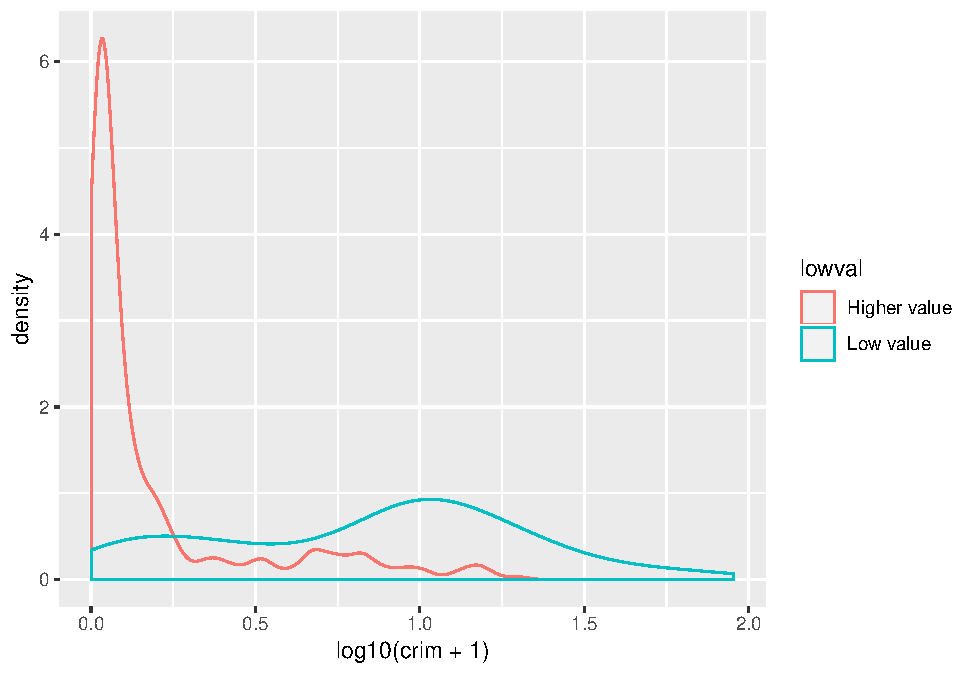
\includegraphics{03-visualisation_files/figure-latex/unnamed-chunk-24-1.pdf}

In a density plot, we attempt to visualize the underlying probability
distribution of the data by drawing an appropriate continuous curve. So
in a density plot then the area under the lines sum to 1 and the Y,
vertical, axis now gives you the estimated (guessed) probability for the
different values in the X, horizontal, axis. This curve is guessed from
the data and the method we use for this guessing or estimation is called
kernel density estimation. You can read more about density plots
\href{https://serialmentor.com/dataviz/histograms-density-plots.html}{here}.

In this plot we can see that there is a high estimated probability of
observing a town with near zero per capita crime rate and a low
estimated probability of seeing towns with large per capita crime rates.
As you can observe it provides a smoother representation of the
distribution (as compared to the histograms).

You can also use this to compare the distribution of a quantitative
variable across the levels in a categorical variable (factor) and, as
before, is possibly better to take the log of skewed variables such as
crime:

\begin{Shaded}
\begin{Highlighting}[]
\CommentTok{#We are mapping "lowval" as the variable colouring the lines }
\KeywordTok{ggplot}\NormalTok{(Boston, }\KeywordTok{aes}\NormalTok{(}\DataTypeTok{x =} \KeywordTok{log10}\NormalTok{(crim }\OperatorTok{+}\StringTok{ }\DecValTok{1}\NormalTok{), }\DataTypeTok{colour =}\NormalTok{ lowval)) }\OperatorTok{+}\StringTok{ }
\StringTok{  }\KeywordTok{geom_density}\NormalTok{() }
\end{Highlighting}
\end{Shaded}

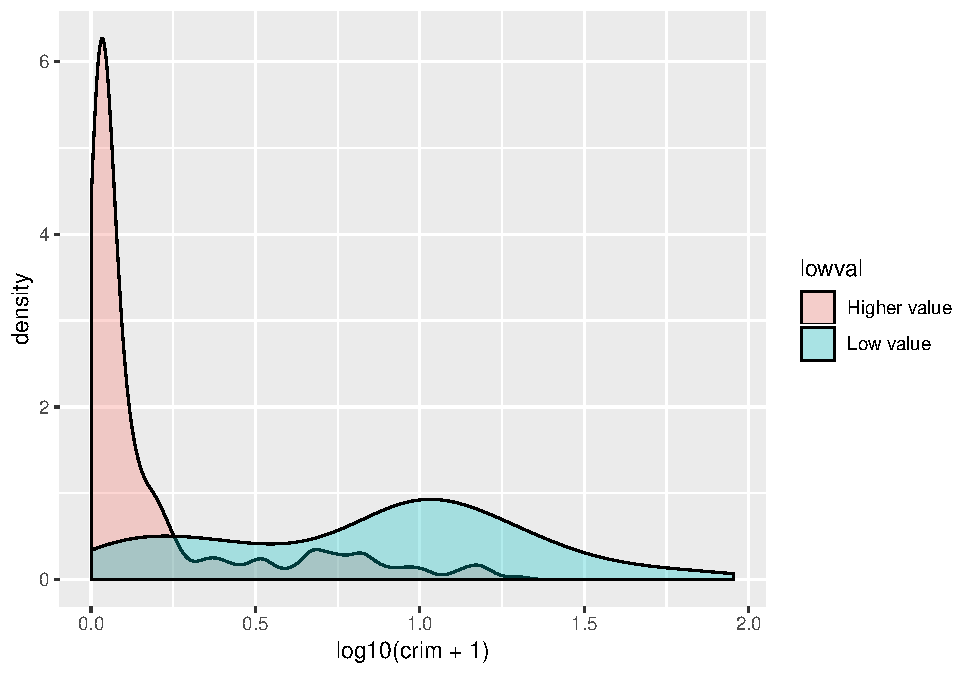
\includegraphics{03-visualisation_files/figure-latex/unnamed-chunk-25-1.pdf}

Or you could use transparencies:

\begin{Shaded}
\begin{Highlighting}[]
\KeywordTok{ggplot}\NormalTok{(Boston, }\KeywordTok{aes}\NormalTok{(}\DataTypeTok{x =} \KeywordTok{log10}\NormalTok{(crim }\OperatorTok{+}\StringTok{ }\DecValTok{1}\NormalTok{), }\DataTypeTok{fill =}\NormalTok{ lowval)) }\OperatorTok{+}\StringTok{ }
\StringTok{  }\KeywordTok{geom_density}\NormalTok{(}\DataTypeTok{alpha =} \FloatTok{.3}\NormalTok{)}
\end{Highlighting}
\end{Shaded}

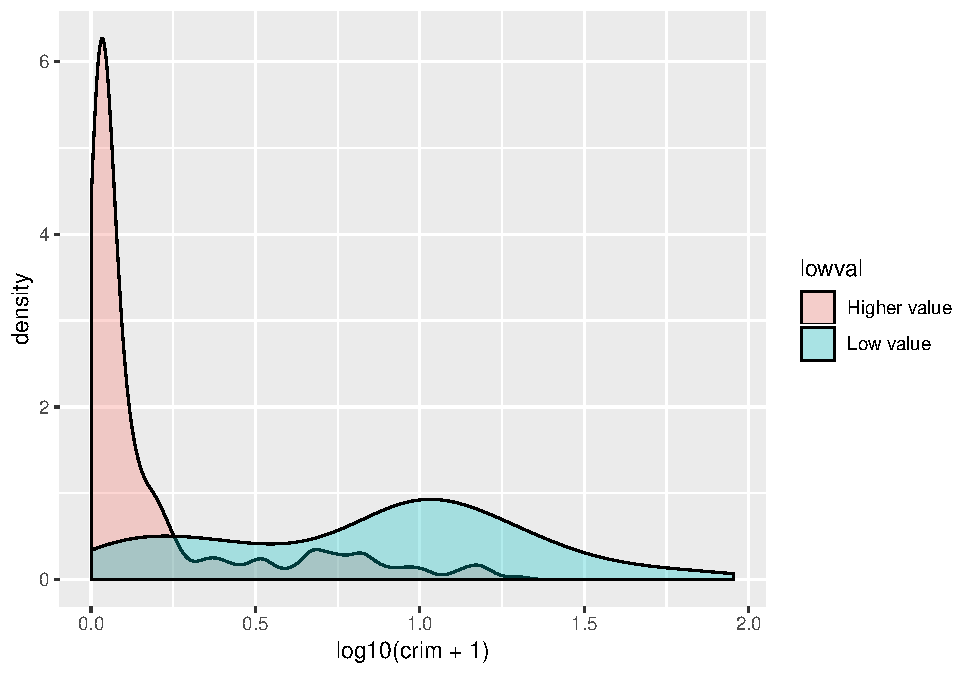
\includegraphics{03-visualisation_files/figure-latex/unnamed-chunk-26-1.pdf}

Did you notice the difference with the comparative histograms? By using
density plots we are rescaling to ensure the same area for each of the
levels in our grouping variable. This makes it easier to compare two
groups that have different frequencies. The areas under the curve add up
to 1 for both of the groups, whereas in the histogram the area within
the bars represent the number of cases in each of the groups. If you
have many more cases in one group than the other it may be difficult to
make comparisons or to clearly see the distribution for the group with
fewer cases. So, this is one of the reasons why you may want to use
density plots.

Density plots are a good choice when you want to compare up to three
groups. If you have many more groups you may want to consider other
alternatives. One such alternative is the ridgeline plot, also often
called the Joy Division plot (since it was immortalised in the cover of
one of their albums):


\includegraphics{imgs/joydivision.png}

They can be produced with the \texttt{ggridges} package. BEfore we
dichotomised the variable medv in a manual way, we can use more direct
ways of splitting nummerica variables into various categories using
information already embedded on them. Say we want to split medv into
deciles. We could use the \texttt{mutate} function in dplyr for this.

\begin{Shaded}
\begin{Highlighting}[]
\KeywordTok{library}\NormalTok{(dplyr)}
\end{Highlighting}
\end{Shaded}

\begin{verbatim}
## 
## Attaching package: 'dplyr'
\end{verbatim}

\begin{verbatim}
## The following object is masked from 'package:MASS':
## 
##     select
\end{verbatim}

\begin{verbatim}
## The following objects are masked from 'package:stats':
## 
##     filter, lag
\end{verbatim}

\begin{verbatim}
## The following objects are masked from 'package:base':
## 
##     intersect, setdiff, setequal, union
\end{verbatim}

\begin{Shaded}
\begin{Highlighting}[]
\NormalTok{Boston <-}\StringTok{ }\KeywordTok{mutate}\NormalTok{(Boston, }\DataTypeTok{dec_medv =} \KeywordTok{ntile}\NormalTok{(medv, }\DecValTok{10}\NormalTok{))}
\end{Highlighting}
\end{Shaded}

The \texttt{mutate} function adds a new variable to our existing data
frame object. We are naming this variable dec\_medv because we are going
to split medv into ten groups of equal size. To do this we will use the
\texttt{ntile} function as an argument within mutate. We will define the
new dec\_medv variable explaining to R that this variable will be the
result of passing the \texttt{ntile} function to medv. So that
\texttt{ntile} breaks medv into 10 we pass this value as an argument to
the function. So that the result of executing \texttt{mutate} are stored
we assign this to the Boston object.

Check the results:

\begin{Shaded}
\begin{Highlighting}[]
\KeywordTok{table}\NormalTok{(Boston}\OperatorTok{$}\NormalTok{dec_medv)}
\end{Highlighting}
\end{Shaded}

\begin{verbatim}
## 
##  1  2  3  4  5  6  7  8  9 10 
## 51 51 50 51 50 51 51 50 51 50
\end{verbatim}

We can now use this new variable to illustrate the use of the
\texttt{ggridge} package. First you will need to install this package
and then load it. You will see all this package does is to extend the
functionality of ggplot by adding a new type of geom. Here the variable
defining the groups needs to be a factor, so we will tell ggplot to
treat dec\_medv as a factor using \texttt{as.factor}.

\begin{Shaded}
\begin{Highlighting}[]
\KeywordTok{library}\NormalTok{(ggridges)}
\end{Highlighting}
\end{Shaded}

\begin{verbatim}
## 
## Attaching package: 'ggridges'
\end{verbatim}

\begin{verbatim}
## The following object is masked from 'package:ggplot2':
## 
##     scale_discrete_manual
\end{verbatim}

\begin{Shaded}
\begin{Highlighting}[]
\KeywordTok{ggplot}\NormalTok{(Boston, }\KeywordTok{aes}\NormalTok{(}\DataTypeTok{x =} \KeywordTok{log10}\NormalTok{(crim }\OperatorTok{+}\StringTok{ }\DecValTok{1}\NormalTok{), }\DataTypeTok{y =} \KeywordTok{as.factor}\NormalTok{(dec_medv))) }\OperatorTok{+}\StringTok{ }\KeywordTok{geom_density_ridges}\NormalTok{()}
\end{Highlighting}
\end{Shaded}

\begin{verbatim}
## Picking joint bandwidth of 0.072
\end{verbatim}

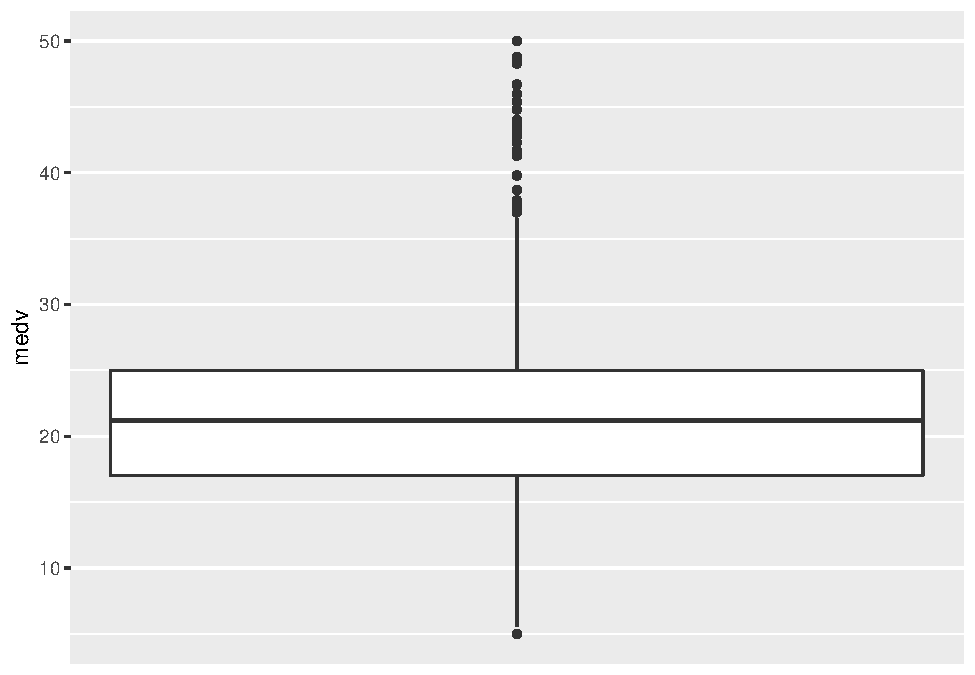
\includegraphics{03-visualisation_files/figure-latex/unnamed-chunk-29-1.pdf}

We can see that the distribution of crime is particularly different when
we focus in the three deciles with the lowest level of income. For more
details you can read the
\href{https://cran.r-project.org/web/packages/ggridges/vignettes/introduction.html}{vignette}
for this package.

\#\#Box plots

\href{http://tomhopper.me/2014/07/04/the-most-useful-data-plot-youve-never-used/}{Box
plots} are an interesting way of presenting the 5 number summary in a
visual way.
\href{http://www.learner.org/courses/againstallodds/unitpages/unit05.html}{This
video} may help you to understand them better. If we want to use
\texttt{ggplot} for plotting a single numerical variable we need some
convoluted code, since \texttt{ggplot} assumes you want a boxplot to
compare various groups. Therefore we need to set some arbitrary value
for the grouping variable and we also may want to remove the x-axis tick
markers and label.

For this illustration, I am going to display the distribution of the
median value of property in the various towns instead of crime.

\begin{Shaded}
\begin{Highlighting}[]
\KeywordTok{ggplot}\NormalTok{(Boston, }\KeywordTok{aes}\NormalTok{(}\DataTypeTok{x =} \DecValTok{1}\NormalTok{, }\DataTypeTok{y =}\NormalTok{ medv)) }\OperatorTok{+}\StringTok{ }
\StringTok{  }\KeywordTok{geom_boxplot}\NormalTok{() }\OperatorTok{+}
\StringTok{  }\KeywordTok{scale_x_continuous}\NormalTok{(}\DataTypeTok{breaks =} \OtherTok{NULL}\NormalTok{) }\OperatorTok{+}\StringTok{ }\CommentTok{#removes the tick markers from the x axis}
\StringTok{  }\KeywordTok{theme}\NormalTok{(}\DataTypeTok{axis.title.x =} \KeywordTok{element_blank}\NormalTok{())}
\end{Highlighting}
\end{Shaded}

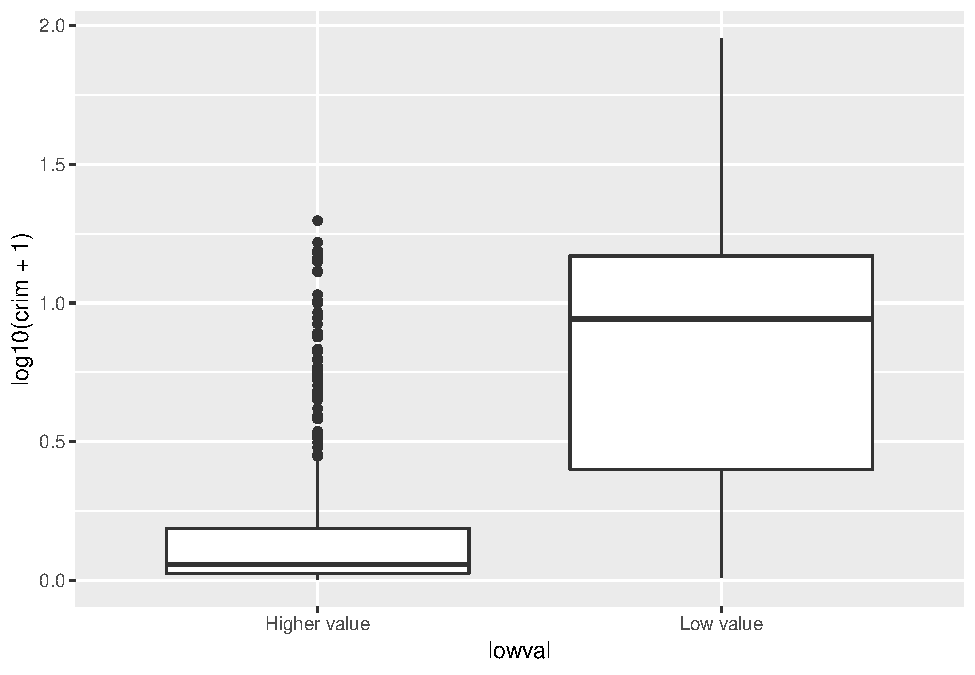
\includegraphics{03-visualisation_files/figure-latex/unnamed-chunk-30-1.pdf}

Boxplots, however, really come to life when you do use them to compare
the distribution of a quantitative variable across various groups. Let's
look at the distribution of log(crime) across cheaper and more expensive
areas:

\begin{Shaded}
\begin{Highlighting}[]
\KeywordTok{ggplot}\NormalTok{(Boston, }\KeywordTok{aes}\NormalTok{(}\DataTypeTok{x =}\NormalTok{ lowval, }\DataTypeTok{y=}\KeywordTok{log10}\NormalTok{(crim }\OperatorTok{+}\StringTok{ }\DecValTok{1}\NormalTok{))) }\OperatorTok{+}
\StringTok{  }\KeywordTok{geom_boxplot}\NormalTok{()}
\end{Highlighting}
\end{Shaded}

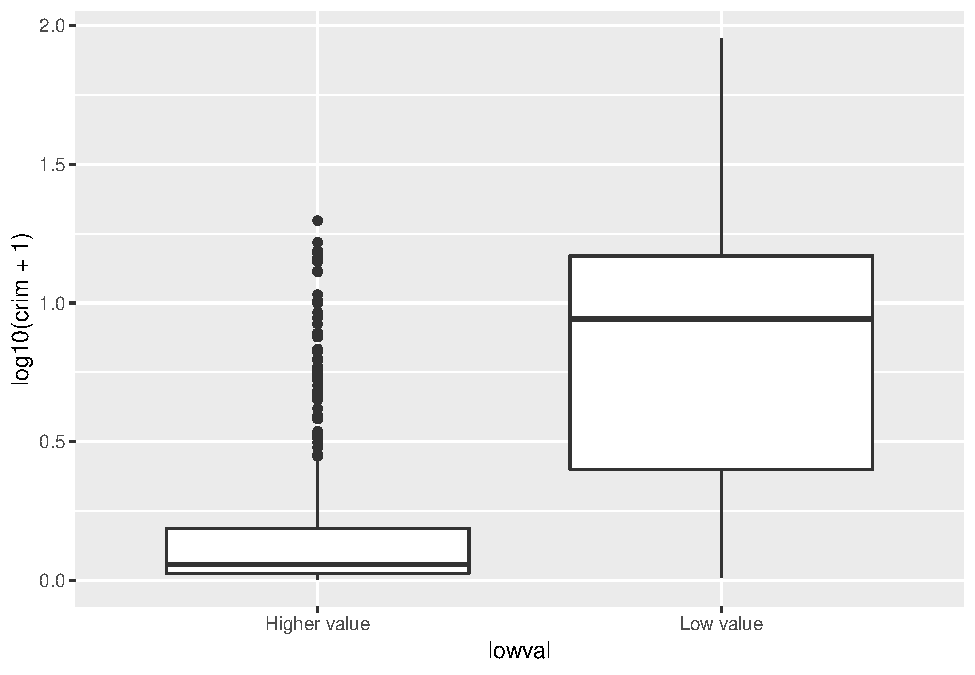
\includegraphics{03-visualisation_files/figure-latex/unnamed-chunk-31-1.pdf}

With a boxplot like this you can see straight away that the bulk of
cheaper areas are very different from the bulk of more expensive areas.
The first quartile of the distribution for low areas about matches the
point at which we start to see \textbf{outliers} for the more expensive
areas.

This can be even more helpful when you have various groups. Let's try an
example using the \texttt{BCS0708} data frame. This is a dataset from
the 207/08 British Crime Survey.You can use the code below to download
it.

\begin{Shaded}
\begin{Highlighting}[]
\CommentTok{##R in Windows have some problems with https addresses, that's why we need to do this first:}
\NormalTok{urlfile<-}\StringTok{'https://raw.githubusercontent.com/jjmedinaariza/LAWS70821/master/BCS0708.csv'}
\CommentTok{#We create a data frame object reading the data from the remote .csv file}
\NormalTok{BCS0708<-}\KeywordTok{read.csv}\NormalTok{(}\KeywordTok{url}\NormalTok{(urlfile))}
\end{Highlighting}
\end{Shaded}

This dataset contains a quantitative variable that measures the level of
worry for crime (\texttt{tcviolent}): high scores represent high levels
of worry. We are going to see how the score in this variable changes
according to ethnicity (\texttt{ethgrp2}).

\begin{Shaded}
\begin{Highlighting}[]
\CommentTok{#A comparative boxplot of ethnicity and worry about violent crime}
\KeywordTok{ggplot}\NormalTok{(BCS0708, }\KeywordTok{aes}\NormalTok{(}\DataTypeTok{x =}\NormalTok{ ethgrp2, }\DataTypeTok{y =}\NormalTok{ tcviolent)) }\OperatorTok{+}
\StringTok{  }\KeywordTok{geom_boxplot}\NormalTok{()}
\end{Highlighting}
\end{Shaded}

\begin{verbatim}
## Warning: Removed 3242 rows containing non-finite values (stat_boxplot).
\end{verbatim}

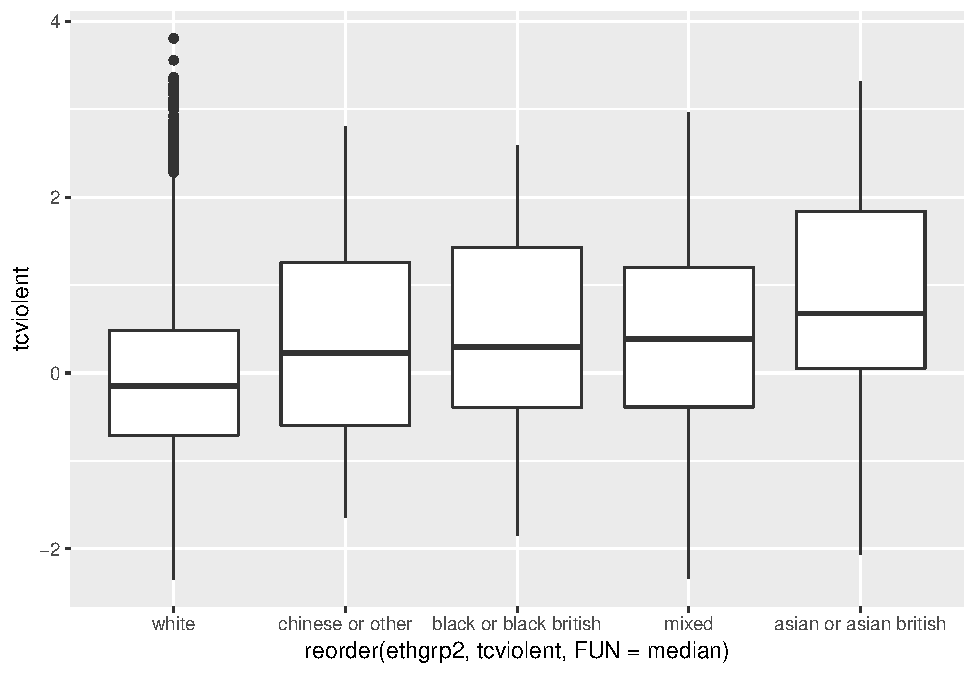
\includegraphics{03-visualisation_files/figure-latex/unnamed-chunk-33-1.pdf}

Nice. But could be nicer. To start with we could order the groups along
the X axis so that the ethnic groups are positioned according to their
level of worry. Secondly, we may want to exclude the information for the
NA cases on ethnicity (represented by a flat line).

\begin{Shaded}
\begin{Highlighting}[]
\CommentTok{#A nicer comparative boxplot (excluding NA and reordering the X variable)}
\KeywordTok{ggplot}\NormalTok{(}\KeywordTok{subset}\NormalTok{(BCS0708, }\OperatorTok{!}\KeywordTok{is.na}\NormalTok{(ethgrp2) }\OperatorTok{&}\StringTok{ }\OperatorTok{!}\KeywordTok{is.na}\NormalTok{(tcviolent)), }
       \KeywordTok{aes}\NormalTok{(}\DataTypeTok{x =} \KeywordTok{reorder}\NormalTok{(ethgrp2, tcviolent, }\DataTypeTok{FUN =}\NormalTok{ median), }\DataTypeTok{y =}\NormalTok{ tcviolent)) }\OperatorTok{+}
\StringTok{        }\KeywordTok{geom_boxplot}\NormalTok{()}
\end{Highlighting}
\end{Shaded}

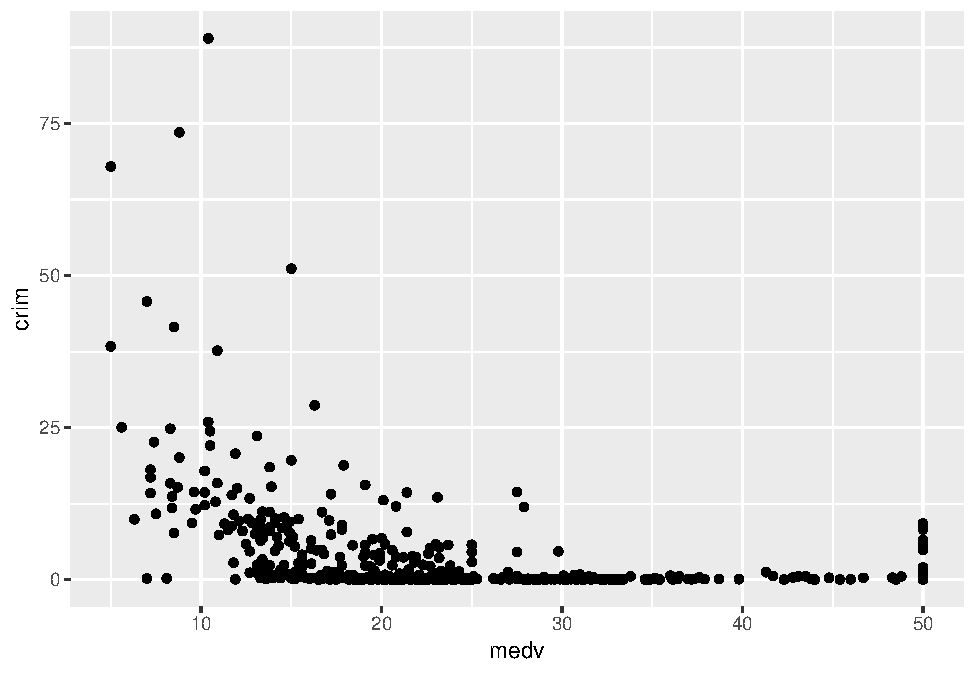
\includegraphics{03-visualisation_files/figure-latex/unnamed-chunk-34-1.pdf}

The \texttt{subset} function is using a logical argument to tell R to
only use the cases that do not have NA values in the two variables that
we are using. The exclamation mark followed by is.na and then the name
of a variable is R way os saying ``the contrary of is NA for the
specified variable''. The \texttt{reorder} function on the other hand is
asking R to reorder the levels in ethnicity according to the median
value of worry of violent crime. Since we are using those functions
\emph{within} the \texttt{ggplot} function this subsetting and this
reordering are not introducing permanent changes in your original
dataset. If you prefer to reorder according to the mean you only need to
change that parameter after the \texttt{FUN} option (e.g,
\texttt{FUN\ =\ mean}).

\#\#Scatter plots with two variables

When looking at the relationship between two quantitative variables
nothing beats the \textbf{scatterplot}.
\href{http://www.datavis.ca/papers/friendly-scat.pdf}{This} is a lovely
article in the history of the scatterplot and
\href{http://www.learner.org/courses/againstallodds/unitpages/unit10.html}{this
video} may help you to understand them better.

A scatterplot plots one variable in the Y axis, and another in the X
axis. Typically, if you have a clear outcome or response variable in
mind, you place it in the Y axis, and you place the explanatory variable
in the X axis.

This is how you produce a scatterplot with \texttt{ggplot()}:

\begin{Shaded}
\begin{Highlighting}[]
\CommentTok{#A scatterplot of crime versus median value of the properties}
\KeywordTok{ggplot}\NormalTok{(Boston, }\KeywordTok{aes}\NormalTok{(}\DataTypeTok{x =}\NormalTok{ medv, }\DataTypeTok{y =}\NormalTok{ crim)) }\OperatorTok{+}
\StringTok{  }\KeywordTok{geom_point}\NormalTok{()}
\end{Highlighting}
\end{Shaded}

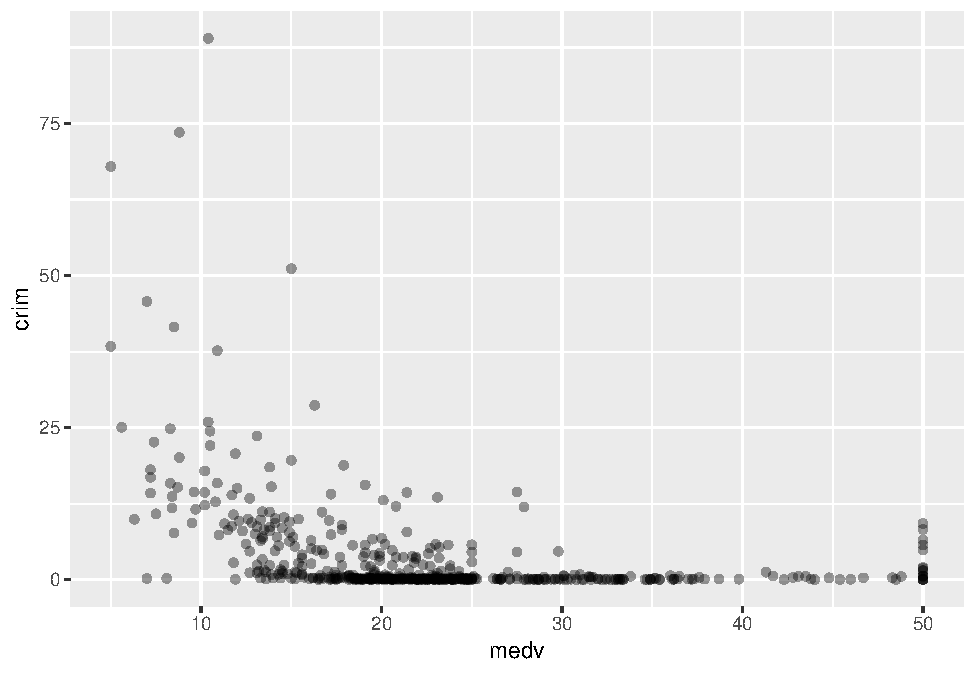
\includegraphics{03-visualisation_files/figure-latex/unnamed-chunk-35-1.pdf}

Each point represents a case in our dataset and the coordinates attached
to it in this two dimensional plane are given by their value in the Y
(crime) and X (median value of the properties) variables.

What do you look for in a scatterplot? You want to assess global and
local patterns, as well as deviations. We can see clearly that at low
levels of \texttt{medv} there is a higher probability in this data that
the level of crime is higher. Once the median value of the property hits
\$30,000 the level of crime is nearly zero for all towns. So far so
good, and surely predictable. The first reason why we look at
scatterplots is to check our hypothesis (e.g., poorer areas, more
crime).

However, something odd seems to be going on when the median property
value is around \$50,000. All of the sudden the variability for crime
goes up. We seem to have some of the more expensive areas also
exhibiting some decent level of crime. What's going on? To be honest I
have no clue (although I have some hypothesis)! This is my first look at
this dataset. But the pattern at the higher level of property value is
indeed odd.

This is the second reason why you want to plot your data before you do
anything else. It helps you to detect apparent anomalies. I say this is
an anomaly because the break in pattern is quite noticeable. It is hard
to think of a natural process that would generate this sudden radical
increase in crime once the median property value reaches the \$50k mark.
If you were analysing this for real, you would want to know what's
driving this pattern (e.g., find out about the original data collection,
the codebook, etc.): perhaps the maximum median value was capped at
\$50K and we are seeing this as a dramatic increase when the picture is
more complex? For now we are going to let this rest.

One of the things you may notice with a scatterplot is that even with a
smallish dataset such as this, with just about 500 cases,
\textbf{overplotting} may be a problem. When you have many cases with
similar (or even worse the same) value, it is difficult to tell them
apart. There's a variety of ways of dealing with overplotting. One
possibility is to add some \textbf{transparency} to the points:

\begin{Shaded}
\begin{Highlighting}[]
\KeywordTok{ggplot}\NormalTok{(Boston, }\KeywordTok{aes}\NormalTok{(}\DataTypeTok{x =}\NormalTok{ medv, }\DataTypeTok{y =}\NormalTok{ crim)) }\OperatorTok{+}
\StringTok{  }\KeywordTok{geom_point}\NormalTok{(}\DataTypeTok{alpha=}\NormalTok{.}\DecValTok{4}\NormalTok{) }\CommentTok{#you will have to test different values for alpha}
\end{Highlighting}
\end{Shaded}

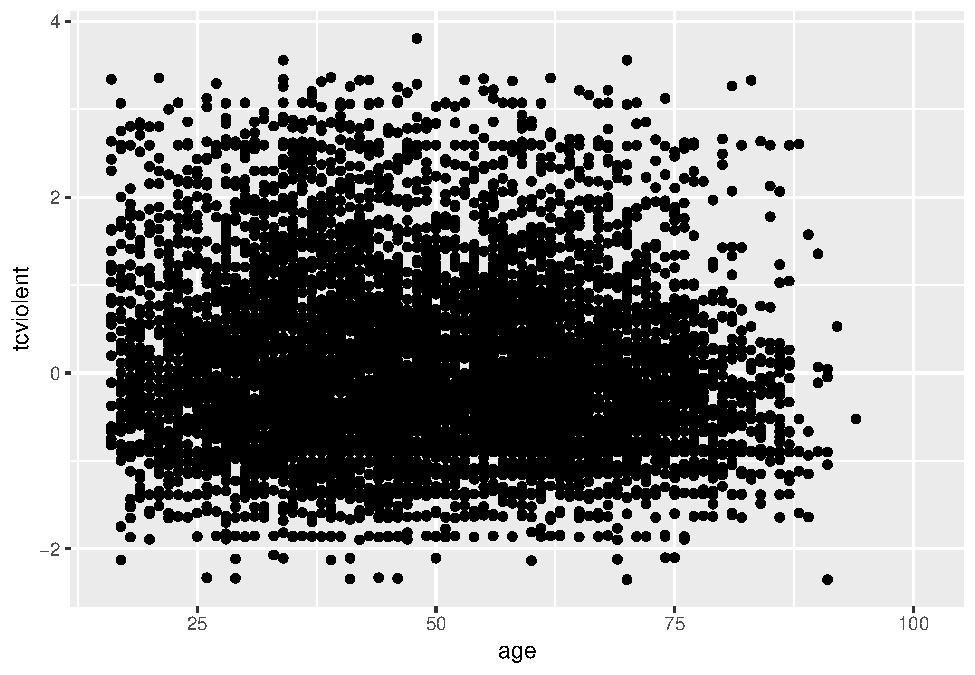
\includegraphics{03-visualisation_files/figure-latex/unnamed-chunk-36-1.pdf}

Why this is an issue may be more evident with the
\texttt{BCS0708\ data}. Compare the two plots:

\begin{Shaded}
\begin{Highlighting}[]
\KeywordTok{ggplot}\NormalTok{(BCS0708, }\KeywordTok{aes}\NormalTok{(}\DataTypeTok{x =}\NormalTok{ age, }\DataTypeTok{y =}\NormalTok{ tcviolent)) }\OperatorTok{+}
\StringTok{  }\KeywordTok{geom_point}\NormalTok{()}
\end{Highlighting}
\end{Shaded}

\begin{verbatim}
## Warning: Removed 3252 rows containing missing values (geom_point).
\end{verbatim}

\includegraphics{03-visualisation_files/figure-latex/unnamed-chunk-37-1.pdf}

\begin{Shaded}
\begin{Highlighting}[]
\KeywordTok{ggplot}\NormalTok{(BCS0708, }\KeywordTok{aes}\NormalTok{(}\DataTypeTok{x =}\NormalTok{ age, }\DataTypeTok{y =}\NormalTok{ tcviolent)) }\OperatorTok{+}
\StringTok{  }\KeywordTok{geom_point}\NormalTok{(}\DataTypeTok{alpha=}\NormalTok{.}\DecValTok{2}\NormalTok{)}
\end{Highlighting}
\end{Shaded}

\begin{verbatim}
## Warning: Removed 3252 rows containing missing values (geom_point).
\end{verbatim}

\includegraphics{03-visualisation_files/figure-latex/unnamed-chunk-38-1.pdf}

The second plot gives us a better idea of where the observations seem to
concentrate in a way that we could not see with the first.

Overplotting can occur when a continuous measurement is rounded to some
convenient unit. This has the effect of changing a continuous variable
into a discrete ordinal variable. For example, age is measured in years
and body weight is measured in pounds or kilograms. Age is a discrete
variable, it only takes integer values. That's why you see the points
lined up in parallel vertical lines. This also contributes to the
overplotting in this case.

One way of dealing with this particular problem is by
\textbf{jittering}. Jittering is the act of adding random noise to data
in order to prevent overplotting in statistical graphs. In
\texttt{ggplot} one way of doing this is by passing an argument to
\texttt{geom\_point} specifying you want to jitter the points. This will
introduce some random noise so that age looks less discrete.

\begin{Shaded}
\begin{Highlighting}[]
\KeywordTok{ggplot}\NormalTok{(BCS0708, }\KeywordTok{aes}\NormalTok{(}\DataTypeTok{x =}\NormalTok{ age, }\DataTypeTok{y =}\NormalTok{ tcviolent)) }\OperatorTok{+}
\StringTok{  }\KeywordTok{geom_point}\NormalTok{(}\DataTypeTok{alpha=}\NormalTok{.}\DecValTok{2}\NormalTok{, }\DataTypeTok{position=}\StringTok{"jitter"}\NormalTok{) }\CommentTok{#Alternatively you could replace geom_point() with geom_jitter() in which case you don't need to specify the position}
\end{Highlighting}
\end{Shaded}

\begin{verbatim}
## Warning: Removed 3252 rows containing missing values (geom_point).
\end{verbatim}

\includegraphics{03-visualisation_files/figure-latex/unnamed-chunk-39-1.pdf}

Another alternative for solving overplotting is to \textbf{bin the data}
into rectangles and map the density of the points to the fill of the
colour of the rectangles.

\begin{Shaded}
\begin{Highlighting}[]
\KeywordTok{ggplot}\NormalTok{(BCS0708, }\KeywordTok{aes}\NormalTok{(}\DataTypeTok{x =}\NormalTok{ age, }\DataTypeTok{y =}\NormalTok{ tcviolent)) }\OperatorTok{+}
\StringTok{  }\KeywordTok{stat_bin2d}\NormalTok{()}
\end{Highlighting}
\end{Shaded}

\begin{verbatim}
## Warning: Removed 3252 rows containing non-finite values (stat_bin2d).
\end{verbatim}

\includegraphics{03-visualisation_files/figure-latex/unnamed-chunk-40-1.pdf}

\begin{Shaded}
\begin{Highlighting}[]
\CommentTok{#The same but with nicer graphical parameters}
\KeywordTok{ggplot}\NormalTok{(BCS0708, }\KeywordTok{aes}\NormalTok{(}\DataTypeTok{x =}\NormalTok{ age, }\DataTypeTok{y =}\NormalTok{ tcviolent)) }\OperatorTok{+}
\StringTok{  }\KeywordTok{stat_bin2d}\NormalTok{(}\DataTypeTok{bins=}\DecValTok{50}\NormalTok{) }\OperatorTok{+}\StringTok{ }\CommentTok{#by increasing the number of bins we get more granularity}
\StringTok{  }\KeywordTok{scale_fill_gradient}\NormalTok{(}\DataTypeTok{low =} \StringTok{"lightblue"}\NormalTok{, }\DataTypeTok{high =} \StringTok{"red"}\NormalTok{) }\CommentTok{#change colors}
\end{Highlighting}
\end{Shaded}

\begin{verbatim}
## Warning: Removed 3252 rows containing non-finite values (stat_bin2d).
\end{verbatim}

\includegraphics{03-visualisation_files/figure-latex/unnamed-chunk-41-1.pdf}

What this is doing is creating boxes within the two dimensional plane;
counting the number of points within those boxes; and attaching a colour
to the box in function of the density of points within each of the
rectangles.

When looking at scatterplots, sometimes it is useful to summarise the
relationships by mean of drawing lines. You could for example add a line
representing the \textbf{conditional mean}. A conditional mean is simply
mean of your Y variable for each value of X. Let's go back to the Boston
dataset. We can ask R to plot a line connecting these means using
\texttt{geom\_line()} and specifying you want the conditional means.

\begin{Shaded}
\begin{Highlighting}[]
\KeywordTok{ggplot}\NormalTok{(Boston, }\KeywordTok{aes}\NormalTok{(}\DataTypeTok{x =}\NormalTok{ medv, }\DataTypeTok{y =}\NormalTok{ crim)) }\OperatorTok{+}
\StringTok{  }\KeywordTok{geom_point}\NormalTok{(}\DataTypeTok{alpha=}\NormalTok{.}\DecValTok{4}\NormalTok{) }\OperatorTok{+}
\StringTok{  }\KeywordTok{geom_line}\NormalTok{(}\DataTypeTok{stat=}\StringTok{'summary'}\NormalTok{, }\DataTypeTok{fun.y=}\NormalTok{mean)}
\end{Highlighting}
\end{Shaded}

\includegraphics{03-visualisation_files/figure-latex/unnamed-chunk-42-1.pdf}

With only about 500 cases there are loads of ups and downs. If you have
many more cases for each level of X the line would look less rough. You
can, in any case, produce a smoother line using \texttt{geom\_smooth}
instead. We will discuss later this semester how this line is computed
(although you will see the R output tells you, you are using something
call the ``loess'' method). For now just know that is a line that tries
to \emph{estimate}, to guess, the typical value for Y for each value of
X.

\begin{Shaded}
\begin{Highlighting}[]
\KeywordTok{ggplot}\NormalTok{(Boston, }\KeywordTok{aes}\NormalTok{(}\DataTypeTok{x =}\NormalTok{ medv, }\DataTypeTok{y =}\NormalTok{ crim)) }\OperatorTok{+}
\StringTok{  }\KeywordTok{geom_point}\NormalTok{(}\DataTypeTok{alpha=}\NormalTok{.}\DecValTok{4}\NormalTok{) }\OperatorTok{+}
\StringTok{  }\KeywordTok{geom_smooth}\NormalTok{(}\DataTypeTok{colour=}\StringTok{"red"}\NormalTok{, }\DataTypeTok{size=}\DecValTok{1}\NormalTok{, }\DataTypeTok{se=}\OtherTok{FALSE}\NormalTok{) }\CommentTok{#We'll explain later this semester what the se argument does, colour is simply asking for a red line instead of blue (which I personally find harder to see. I'm also making the line a bit thicker with size 1)}
\end{Highlighting}
\end{Shaded}

\begin{verbatim}
## `geom_smooth()` using method = 'loess' and formula 'y ~ x'
\end{verbatim}

\includegraphics{03-visualisation_files/figure-latex/unnamed-chunk-43-1.pdf}

As you can see here you produce a smoother line than with the
conditional means. The line, as the scatterplot, seems to be suggesting
an overall curvilinear relationship that almost flattens out once
property values hit \$20k.

\#\#Scatter plots conditioning in a third variable

There are various ways to plot a third variable in a scatterplot. You
could go 3D and in some contexts that may be appropriate. But more often
than not it is preferable to use only a two dimensional plot.

If you have a grouping variable you could map it to the colour of the
points as one of the aesthetics arguments. Here we return to the Boston
scatterplot but will add a third variable, that indicates whether the
town is located by the river or not.

\begin{Shaded}
\begin{Highlighting}[]
\CommentTok{#Scatterplot with two quantitative variables and a grouping variable, we are telling R to tell "chas", a numeric vector, as a factor. }
\KeywordTok{ggplot}\NormalTok{(Boston, }\KeywordTok{aes}\NormalTok{(}\DataTypeTok{x =}\NormalTok{ medv, }\DataTypeTok{y =}\NormalTok{ crim, }\DataTypeTok{colour =} \KeywordTok{as.factor}\NormalTok{(chas))) }\OperatorTok{+}
\StringTok{  }\KeywordTok{geom_point}\NormalTok{() }
\end{Highlighting}
\end{Shaded}

\includegraphics{03-visualisation_files/figure-latex/unnamed-chunk-44-1.pdf}

Curiously, we can see that there's quite a few of those expensive areas
with high levels of crime that seem to be located by the river.

As before you can add smooth lines to capture the relationship. What
happens now, though, is that \texttt{ggplot} will produce a line for
each of the levels in the categorical variable grouping the cases:

\begin{Shaded}
\begin{Highlighting}[]
\KeywordTok{ggplot}\NormalTok{(Boston, }\KeywordTok{aes}\NormalTok{(}\DataTypeTok{x =}\NormalTok{ medv, }\DataTypeTok{y =}\NormalTok{ crim, }\DataTypeTok{colour =} \KeywordTok{as.factor}\NormalTok{(chas))) }\OperatorTok{+}
\StringTok{  }\KeywordTok{geom_point}\NormalTok{(}\DataTypeTok{alpha=}\NormalTok{.}\DecValTok{4}\NormalTok{) }\OperatorTok{+}\StringTok{ }\CommentTok{#I am doing the points semi-transparent to see the lines better}
\StringTok{  }\KeywordTok{geom_smooth}\NormalTok{(}\DataTypeTok{se=}\OtherTok{FALSE}\NormalTok{, }\DataTypeTok{size=}\DecValTok{1}\NormalTok{) }\CommentTok{#I am doing the lines thicker to see them better}
\end{Highlighting}
\end{Shaded}

\begin{verbatim}
## `geom_smooth()` using method = 'loess' and formula 'y ~ x'
\end{verbatim}

\includegraphics{03-visualisation_files/figure-latex/unnamed-chunk-45-1.pdf}

You can see how the relationship between crime and property values is
more marked for areas not bordering the river, mostly because you have
considerably fewer cheaper areas bordering the river. Notice as well the
upward trend in the green line at high values of \texttt{medv}. As we
saw there seems to be quite a few of those particularly more expensive
areas that have high crime and seem to be by the river.

We can also map a quantitative variable to the colour aesthetic. When we
do that, instead of different colours for each category we have a
gradation in colour from darker to lighter depending on the value of the
quantitative variable. Below we display the relationship between crime
and property values conditioning on the status of the area (high values
in \texttt{lstat} represent lower status).

\begin{Shaded}
\begin{Highlighting}[]
\KeywordTok{ggplot}\NormalTok{(Boston, }\KeywordTok{aes}\NormalTok{(}\DataTypeTok{x =}\NormalTok{ medv, }\DataTypeTok{y =}\NormalTok{ crim, }\DataTypeTok{colour =}\NormalTok{ lstat)) }\OperatorTok{+}
\StringTok{  }\KeywordTok{geom_point}\NormalTok{() }
\end{Highlighting}
\end{Shaded}

\includegraphics{03-visualisation_files/figure-latex/unnamed-chunk-46-1.pdf}

As one could predict \texttt{lstat} and \texttt{medv} seem to be
correlated. The areas with low status tend to be the areas with cheaper
properties (and more crime) and the areas with higher status tend to be
the areas with more expensive properties (and less crime).

You could map the third variable to a different aesthetic (rather than
colour). For example, you could map \texttt{lstat} to size of the
points. This is called a \textbf{bubblechart}. The problem with this,
however, is that it can make overplotting more acute sometimes.

\begin{Shaded}
\begin{Highlighting}[]
\KeywordTok{ggplot}\NormalTok{(Boston, }\KeywordTok{aes}\NormalTok{(}\DataTypeTok{x =}\NormalTok{ medv, }\DataTypeTok{y =}\NormalTok{ crim, }\DataTypeTok{size =}\NormalTok{ lstat)) }\OperatorTok{+}
\StringTok{  }\KeywordTok{geom_point}\NormalTok{() }\CommentTok{#You may want to add alpha for some transparency here.}
\end{Highlighting}
\end{Shaded}

\includegraphics{03-visualisation_files/figure-latex/unnamed-chunk-47-1.pdf}

If you have larger samples and the patterns are not clear (as we saw
when looking at the relationship between age and worry of violent crime)
conditioning in a third variable can produce hard to read scatterplots
(even if you use transparencies and jittering). Let's look at the
relationship between worry for violent crime and age conditioned on
victimisation during the previous year:

\begin{Shaded}
\begin{Highlighting}[]
\KeywordTok{ggplot}\NormalTok{(BCS0708, }\KeywordTok{aes}\NormalTok{(}\DataTypeTok{x =}\NormalTok{ age, }\DataTypeTok{y =}\NormalTok{ tcviolent, }\DataTypeTok{colour =}\NormalTok{ bcsvictim)) }\OperatorTok{+}
\StringTok{  }\KeywordTok{geom_point}\NormalTok{(}\DataTypeTok{alpha=}\NormalTok{.}\DecValTok{4}\NormalTok{, }\DataTypeTok{position=}\StringTok{"jitter"}\NormalTok{)}
\end{Highlighting}
\end{Shaded}

\begin{verbatim}
## Warning: Removed 3252 rows containing missing values (geom_point).
\end{verbatim}

\includegraphics{03-visualisation_files/figure-latex/unnamed-chunk-48-1.pdf}

You can possibly notice that there are more green points in the left
hand side (since victimisation tend to be more common among youth). But
it is hard to read the relationship with age. We could try to use facets
instead using \texttt{facet\_grid}?

\begin{Shaded}
\begin{Highlighting}[]
\KeywordTok{ggplot}\NormalTok{(BCS0708, }\KeywordTok{aes}\NormalTok{(}\DataTypeTok{x =}\NormalTok{ age, }\DataTypeTok{y =}\NormalTok{ tcviolent)) }\OperatorTok{+}
\StringTok{  }\KeywordTok{geom_point}\NormalTok{(}\DataTypeTok{alpha=}\NormalTok{.}\DecValTok{4}\NormalTok{, }\DataTypeTok{position=}\StringTok{"jitter"}\NormalTok{) }\OperatorTok{+}
\StringTok{  }\KeywordTok{facet_grid}\NormalTok{( .}\OperatorTok{~}\StringTok{ }\NormalTok{bcsvictim)}
\end{Highlighting}
\end{Shaded}

\begin{verbatim}
## Warning: Removed 3252 rows containing missing values (geom_point).
\end{verbatim}

\includegraphics{03-visualisation_files/figure-latex/unnamed-chunk-49-1.pdf}

It is still hard to see anything, though perhaps you can notice the
lower density the points in the bottom right corner in the facet
displaying victims of crime. In a case like this may be helpful to draw
a smooth line

\begin{Shaded}
\begin{Highlighting}[]
\KeywordTok{ggplot}\NormalTok{(BCS0708, }\KeywordTok{aes}\NormalTok{(}\DataTypeTok{x =}\NormalTok{ age, }\DataTypeTok{y =}\NormalTok{ tcviolent, }\DataTypeTok{colour =}\NormalTok{ bcsvictim)) }\OperatorTok{+}
\StringTok{  }\KeywordTok{geom_point}\NormalTok{(}\DataTypeTok{alpha=}\NormalTok{.}\DecValTok{1}\NormalTok{, }\DataTypeTok{position=}\StringTok{"jitter"}\NormalTok{) }\OperatorTok{+}
\StringTok{  }\KeywordTok{geom_smooth}\NormalTok{(}\DataTypeTok{size=}\FloatTok{1.5}\NormalTok{, }\DataTypeTok{se=}\OtherTok{FALSE}\NormalTok{)}
\end{Highlighting}
\end{Shaded}

\begin{verbatim}
## `geom_smooth()` using method = 'gam' and formula 'y ~ s(x, bs = "cs")'
\end{verbatim}

\begin{verbatim}
## Warning: Removed 3252 rows containing non-finite values (stat_smooth).
\end{verbatim}

\begin{verbatim}
## Warning: Removed 3252 rows containing missing values (geom_point).
\end{verbatim}

\includegraphics{03-visualisation_files/figure-latex/unnamed-chunk-50-1.pdf}

What we see here is that for the most part the relationship of age and
worry for violent crime looks quite flat, regardless of whether you have
been a victim of crime or not. At least, for most people. However, once
we get to the 60s things seem to change a bit. Those over 62 that have
not been a victim of crime in the past year start to manifest a lower
concern with crime as they age (in comparison with those that have been
a victim of crime).

\#\#Scatterplot matrix

Sometimes you want to produce many scatterplots simultaneously to have a
first peak at the relationship between the various variables in your
data frame. The way to do this is by using a scatterplot matrix.
Unfortunately, \texttt{ggplot2} doesn't do scatterplot matrix too well.
For this it is better to use the graphics tools of base R.

Not to overcomplicate things we will only use a few variables from the
\texttt{Boston} dataset:

\begin{Shaded}
\begin{Highlighting}[]
\CommentTok{#I create a new data frame that only contains 4 variables included in the Boston dataset and I am calling this new data frame object BostonSM}
\NormalTok{Boston_SM <-}\StringTok{ }\KeywordTok{subset}\NormalTok{(Boston, }\DataTypeTok{select =} \KeywordTok{c}\NormalTok{(crim, medv, indus, lstat))}
\end{Highlighting}
\end{Shaded}

Then we run the scatterplot matrix using the \textbf{pairs()} function:

\begin{Shaded}
\begin{Highlighting}[]
\KeywordTok{pairs}\NormalTok{(Boston_SM)}
\end{Highlighting}
\end{Shaded}

\includegraphics{03-visualisation_files/figure-latex/unnamed-chunk-52-1.pdf}

We can modify this code to put additional information in the matrix. As
you may have noticed the matrix is symmetrical, for every scatterplot in
the upper left side there is a similar on the the bottom right side. We
are going to modify this matrix so that the diagonal boxes not only
display the name of the variable but also a histogram for the variables
and to display the correlation coefficients in the upper left side
(instead of printing twice the same scatterplot). We will also make the
points smaller and will add a smooth line within each scatterplot.

The code for this is a bit complicated. We are going to introduce
\textbf{customised functions} for the panels (I took them from Winston
Chang book). First we are going to create these two customised
functions. One to produce the correlations between each pair of
variables and another for producing the histograms for each of the
variables.

After that we will use the \texttt{pairs()} function inserting the
inputs that result form using these customised functions. You are likely
not to understand the code for the first part. Particularly because
apart from doing computations is controlling the aspect of the results.
Don't worry, I'm not expecting to understand this code. Just cut and
paste. But I think it is important you understand that apart from using
the functions created by others and included in packages, once you
become proficient in R you can start producing your own functions to
expand the range of what you can do with R.

\begin{Shaded}
\begin{Highlighting}[]
\NormalTok{panel.cor <-}\StringTok{ }\ControlFlowTok{function}\NormalTok{(x, y, }\DataTypeTok{digits=}\DecValTok{2}\NormalTok{, }\DataTypeTok{prefix=}\StringTok{""}\NormalTok{, cex.cor, ...)\{}
\NormalTok{  usr <-}\StringTok{ }\KeywordTok{par}\NormalTok{(}\StringTok{"usr"}\NormalTok{)}
  \KeywordTok{on.exit}\NormalTok{(}\KeywordTok{par}\NormalTok{(usr))}
  \KeywordTok{par}\NormalTok{(}\DataTypeTok{usr =} \KeywordTok{c}\NormalTok{(}\DecValTok{0}\NormalTok{, }\DecValTok{1}\NormalTok{, }\DecValTok{0}\NormalTok{, }\DecValTok{1}\NormalTok{))}
\NormalTok{  r <-}\StringTok{ }\KeywordTok{abs}\NormalTok{(}\KeywordTok{cor}\NormalTok{(x, y, }\DataTypeTok{use=}\StringTok{"complete.obs"}\NormalTok{))}
\NormalTok{  txt <-}\StringTok{ }\KeywordTok{format}\NormalTok{(}\KeywordTok{c}\NormalTok{(r, }\FloatTok{0.123456789}\NormalTok{), }\DataTypeTok{digits=}\NormalTok{digits)[}\DecValTok{1}\NormalTok{]}
\NormalTok{  txt <-}\StringTok{ }\KeywordTok{paste}\NormalTok{(prefix, txt, }\DataTypeTok{sep=}\StringTok{""}\NormalTok{)}
  \ControlFlowTok{if}\NormalTok{(}\KeywordTok{missing}\NormalTok{(cex.cor)) cex.cor <-}\StringTok{ }\FloatTok{0.8}\OperatorTok{/}\KeywordTok{strwidth}\NormalTok{(txt)}
  \KeywordTok{text}\NormalTok{(}\FloatTok{0.5}\NormalTok{, }\FloatTok{0.5}\NormalTok{, txt, }\DataTypeTok{cex =}\NormalTok{ cex.cor }\OperatorTok{*}\StringTok{ }\NormalTok{(}\DecValTok{1}\OperatorTok{+}\NormalTok{r)}\OperatorTok{/}\DecValTok{2}\NormalTok{)}
\NormalTok{\}}
\NormalTok{panel.hist <-}\ControlFlowTok{function}\NormalTok{(x, ...)\{}
\NormalTok{  usr <-}\StringTok{ }\KeywordTok{par}\NormalTok{(}\StringTok{"usr"}\NormalTok{)}
  \KeywordTok{on.exit}\NormalTok{(}\KeywordTok{par}\NormalTok{(usr))}
  \KeywordTok{par}\NormalTok{(}\DataTypeTok{usr =} \KeywordTok{c}\NormalTok{(usr[}\DecValTok{1}\OperatorTok{:}\DecValTok{2}\NormalTok{], }\DecValTok{0}\NormalTok{, }\FloatTok{1.5}\NormalTok{))}
\NormalTok{  h <-}\StringTok{ }\KeywordTok{hist}\NormalTok{(x, }\DataTypeTok{plot =} \OtherTok{FALSE}\NormalTok{)}
\NormalTok{  breaks <-}\StringTok{ }\NormalTok{h}\OperatorTok{$}\NormalTok{breaks}
\NormalTok{  nB <-}\StringTok{ }\KeywordTok{length}\NormalTok{(breaks)}
\NormalTok{  y <-}\StringTok{ }\NormalTok{h}\OperatorTok{$}\NormalTok{counts}
\NormalTok{  y <-}\StringTok{ }\NormalTok{y}\OperatorTok{/}\KeywordTok{max}\NormalTok{(y)}
  \KeywordTok{rect}\NormalTok{(breaks[}\OperatorTok{-}\NormalTok{nB], }\DecValTok{0}\NormalTok{, breaks[}\OperatorTok{-}\DecValTok{1}\NormalTok{], y, }\DataTypeTok{col=}\StringTok{"white"}\NormalTok{, ...)}
\NormalTok{\}}
\end{Highlighting}
\end{Shaded}

We can now run the \texttt{pairs()} function using our customised
functions as inputs.

\begin{Shaded}
\begin{Highlighting}[]
\KeywordTok{pairs}\NormalTok{(Boston_SM, }\DataTypeTok{pch=}\StringTok{"."}\NormalTok{, }\CommentTok{#Produces smaller points to make it easier to see}
      \DataTypeTok{upper.panel=}\NormalTok{panel.smooth, }\CommentTok{#Adds for smoothed lines to be added to the lower panel scatterplots }
      \DataTypeTok{lower.panel=}\NormalTok{panel.cor, }\CommentTok{#Ask for correlation coeffients in the upper panel using our customised functions (the size of the numer is bigger is the correlation is bigger, but notice that the coefficient does not include the sign, whether is positve or negative, you need to infer that from the scatterplot)}
      \DataTypeTok{diag.panel=}\NormalTok{panel.hist) }\CommentTok{#Ask for histograms in the diagonal using our customised function}
\end{Highlighting}
\end{Shaded}

\includegraphics{03-visualisation_files/figure-latex/unnamed-chunk-54-1.pdf}

We will explain what correlation coefficients are and when they are
appropriate later this semester. For now just focus in trying to
understand what the plots show. What do you think may be going on with
the distribution of ``indus'' (proportion of non-retail business acres
per town)?

As you can see getting results, once you get the knack of it, is only
half of the way. The other, and more important, half is trying to make
sense of the results. R cannot do that for you. For this you need to use
a better tool: \textbf{your brain} (scepticism, curiosity, creativity, a
lifetime of knowledge) and what Kaiser Fung calls
\href{http://www.amazon.co.uk/Numbersense-How-Data-Your-Advantage/dp/0071799664}{``numbersense''}.

\#\#Titles and legends in ggplot2

We have introduced a number of various graphical tools, but what if you
want to customise the way the produce graphic looks like? Here I am just
going to give you some code for how to modify the titles and legends you
use. For adding a title for a \texttt{ggplot} graph you use
\texttt{ggtitle()}.

\begin{Shaded}
\begin{Highlighting}[]
\CommentTok{#Notice how here we are using an additional function to ask R to treat the variable chas, which is numeric in our dataset, as if it were a factor (as.factor()). You need to do this if your variable is categorical but is encoded as numeric in your dataframe.}
\KeywordTok{ggplot}\NormalTok{(Boston, }\KeywordTok{aes}\NormalTok{(}\DataTypeTok{x =}\NormalTok{ medv, }\DataTypeTok{y =}\NormalTok{ crim, }\DataTypeTok{colour =} \KeywordTok{as.factor}\NormalTok{(chas))) }\OperatorTok{+}
\StringTok{  }\KeywordTok{geom_point}\NormalTok{() }\OperatorTok{+}
\StringTok{  }\KeywordTok{ggtitle}\NormalTok{(}\StringTok{"Fig 1.Crime, Property Value and River Proximity of Boston Towns"}\NormalTok{)}
\end{Highlighting}
\end{Shaded}

\includegraphics{03-visualisation_files/figure-latex/unnamed-chunk-55-1.pdf}

If you don't like the default background theme for \texttt{ggplot} you
can use a theme as discussed at the start, for example with creating a
black and white background by adding \texttt{theme\_bw()} as a layer:

\begin{Shaded}
\begin{Highlighting}[]
\KeywordTok{ggplot}\NormalTok{(Boston, }\KeywordTok{aes}\NormalTok{(}\DataTypeTok{x =}\NormalTok{ medv, }\DataTypeTok{y =}\NormalTok{ crim, }\DataTypeTok{colour =} \KeywordTok{as.factor}\NormalTok{(chas))) }\OperatorTok{+}
\StringTok{  }\KeywordTok{geom_point}\NormalTok{() }\OperatorTok{+}
\StringTok{  }\KeywordTok{ggtitle}\NormalTok{(}\StringTok{"Fig 1.Crime, Property Value and River Proximity of Boston Towns"}\NormalTok{) }\OperatorTok{+}
\StringTok{  }\KeywordTok{theme_bw}\NormalTok{()}
\end{Highlighting}
\end{Shaded}

\includegraphics{03-visualisation_files/figure-latex/unnamed-chunk-56-1.pdf}

Using \texttt{labs()} you can change the text of axis labels (and the
legend title), which may be handy if your variables have cryptic names.
Equally you can manually name the labels in a legend. The value for
``chas'' are 0 and 1. This is not informative. We can change that.

\begin{Shaded}
\begin{Highlighting}[]
\KeywordTok{ggplot}\NormalTok{(Boston, }\KeywordTok{aes}\NormalTok{(}\DataTypeTok{x =}\NormalTok{ medv, }\DataTypeTok{y =}\NormalTok{ crim, }\DataTypeTok{colour =} \KeywordTok{as.factor}\NormalTok{(chas))) }\OperatorTok{+}
\StringTok{  }\KeywordTok{geom_point}\NormalTok{() }\OperatorTok{+}
\StringTok{  }\KeywordTok{ggtitle}\NormalTok{(}\StringTok{"Fig 1.Crime, Property Value and River Proximity of Boston Towns"}\NormalTok{) }\OperatorTok{+}
\StringTok{  }\KeywordTok{labs}\NormalTok{(}\DataTypeTok{x =} \StringTok{"Median Property Value (in US Dollars x 1000)"}\NormalTok{,}
       \DataTypeTok{y =} \StringTok{"Per capita crime rate"}\NormalTok{,}
       \DataTypeTok{colour =} \StringTok{"Borders the river"}\NormalTok{) }\OperatorTok{+}
\StringTok{  }\KeywordTok{scale_colour_discrete}\NormalTok{(}\DataTypeTok{labels =} \KeywordTok{c}\NormalTok{(}\StringTok{"No"}\NormalTok{, }\StringTok{"Yes"}\NormalTok{))}
\end{Highlighting}
\end{Shaded}

\includegraphics{03-visualisation_files/figure-latex/unnamed-chunk-57-1.pdf}

Sometimes you may want to present several plots together. For this the
\texttt{gridExtra} package is very good. You will first need to install
it and then load it. You can then create several plots and put them all
in the same image.

\begin{Shaded}
\begin{Highlighting}[]
\CommentTok{#You may need to install first with install.packages("gridExtra")}
\KeywordTok{library}\NormalTok{(gridExtra)}
\end{Highlighting}
\end{Shaded}

\begin{verbatim}
## 
## Attaching package: 'gridExtra'
\end{verbatim}

\begin{verbatim}
## The following object is masked from 'package:dplyr':
## 
##     combine
\end{verbatim}

\begin{Shaded}
\begin{Highlighting}[]
\CommentTok{#Store your plots in various objects}
\NormalTok{p1 <-}\StringTok{ }\KeywordTok{qplot}\NormalTok{(}\DataTypeTok{x=}\NormalTok{crim, }\DataTypeTok{data=}\NormalTok{Boston)}
\NormalTok{p2 <-}\StringTok{ }\KeywordTok{qplot}\NormalTok{(}\DataTypeTok{x=}\NormalTok{indus, }\DataTypeTok{data=}\NormalTok{Boston)}
\NormalTok{p3 <-}\StringTok{ }\KeywordTok{qplot}\NormalTok{(}\DataTypeTok{x=}\NormalTok{medv, }\DataTypeTok{data=}\NormalTok{Boston)}
\CommentTok{#Then put them all together using grid.arrange()}
\KeywordTok{grid.arrange}\NormalTok{(p1, p2, p3, }\DataTypeTok{ncol=}\DecValTok{3}\NormalTok{) }\CommentTok{#ncol tells R we want them side by side, if you want them one in top of the other try ncol=1, in this case, however ncol=2 would possibly be the better solution. Try it!}
\end{Highlighting}
\end{Shaded}

\begin{verbatim}
## `stat_bin()` using `bins = 30`. Pick better value with `binwidth`.
\end{verbatim}

\begin{verbatim}
## `stat_bin()` using `bins = 30`. Pick better value with `binwidth`.
## `stat_bin()` using `bins = 30`. Pick better value with `binwidth`.
\end{verbatim}

\includegraphics{03-visualisation_files/figure-latex/unnamed-chunk-58-1.pdf}

\#\#Plotting categorical data: bar charts

You may be wondering what about categorical data? So far we have only
discussed various visualisations where at least one of your variables is
quantitative. When your variable is categorical you can use bar plots
(similar to histograms). We map the factor variable in the aesthetics
and then use the \texttt{geom\_bar()} function to ask for a bar chart.

\begin{Shaded}
\begin{Highlighting}[]
\KeywordTok{ggplot}\NormalTok{(BCS0708, }\KeywordTok{aes}\NormalTok{(}\DataTypeTok{x=}\NormalTok{walkday)) }\OperatorTok{+}
\StringTok{  }\KeywordTok{geom_bar}\NormalTok{()}
\end{Highlighting}
\end{Shaded}

\includegraphics{03-visualisation_files/figure-latex/unnamed-chunk-59-1.pdf}

Unfortunately, the levels in this factor are ordered by alphabetical
order, which is confusing. We can modify this by reordering the factors
levels first -click
\href{http://www.cookbook-r.com/Manipulating_data/Changing_the_order_of_levels_of_a_factor/}{here}
for more details. You could do this within the ggplot function (just for
the visualisation), but in real life you would want to sort out your
factor levels in an appropriate manner more permanently. As discussed
last week, this is the sort of thing you do as part of pre-processing
your data. And then plot.

\begin{Shaded}
\begin{Highlighting}[]
\CommentTok{#Print the original order}
\KeywordTok{print}\NormalTok{(}\KeywordTok{levels}\NormalTok{(BCS0708}\OperatorTok{$}\NormalTok{walkday))}
\end{Highlighting}
\end{Shaded}

\begin{verbatim}
## [1] "a bit unsafe"   "fairly safe"    "or very unsafe" "very safe"
\end{verbatim}

\begin{Shaded}
\begin{Highlighting}[]
\CommentTok{#Reordering the factor levels from very safe to very unsafe (rather than by alphabet). Notice that I am creating a new variable, it is often not unwise to do this to avoid messing up your original data.}
\NormalTok{BCS0708}\OperatorTok{$}\NormalTok{walkdayR <-}\StringTok{ }\KeywordTok{factor}\NormalTok{(BCS0708}\OperatorTok{$}\NormalTok{walkday, }\DataTypeTok{levels=}\KeywordTok{c}\NormalTok{(}\StringTok{'very safe'}\NormalTok{,}
  \StringTok{'fairly safe'}\NormalTok{,}\StringTok{'a bit unsafe'}\NormalTok{,}\StringTok{'or very unsafe'}\NormalTok{))}
\CommentTok{#Plotting the variable again (and subsetting out the NA data)}
\KeywordTok{ggplot}\NormalTok{(}\KeywordTok{subset}\NormalTok{(BCS0708, }\OperatorTok{!}\KeywordTok{is.na}\NormalTok{(walkdayR)), }\KeywordTok{aes}\NormalTok{(}\DataTypeTok{x=}\NormalTok{walkdayR)) }\OperatorTok{+}
\StringTok{  }\KeywordTok{geom_bar}\NormalTok{()}
\end{Highlighting}
\end{Shaded}

\includegraphics{03-visualisation_files/figure-latex/unnamed-chunk-61-1.pdf}

We can also map a second variable to the aesthetics, for example, let's
look at victimisation in relation to feelings of safety. For this we
produce a \textbf{stacked bar chart}.

\begin{Shaded}
\begin{Highlighting}[]
\KeywordTok{ggplot}\NormalTok{(}\KeywordTok{subset}\NormalTok{(BCS0708, }\OperatorTok{!}\KeywordTok{is.na}\NormalTok{(walkdayR)), }\KeywordTok{aes}\NormalTok{(}\DataTypeTok{x=}\NormalTok{walkdayR, }\DataTypeTok{fill=}\NormalTok{bcsvictim)) }\OperatorTok{+}
\StringTok{  }\KeywordTok{geom_bar}\NormalTok{()}
\end{Highlighting}
\end{Shaded}

\includegraphics{03-visualisation_files/figure-latex/unnamed-chunk-62-1.pdf}

These sort of stacked bar charts are not terribly helpful if you are
interested in understanding the relationship between these two
variables. Instead what you want is a \textbf{proportional stacked bar
chart}, that gives you the proportion of your ``explanatory variable''
(here victimisation in the past 12 months) within each of the levels of
your ``response variable'' (here feelings of safety).

First we need to scale the data to 100\% within each stack and then
plot. The code here is also more complex. Again, I'm not expecting you
to fully understand all of it. In your early days of using R, you will
find yourself cutting and pasting chunks of code that you will only
fully understand with practice.

\begin{Shaded}
\begin{Highlighting}[]
\CommentTok{#First we create a subset with the relevant data}
\NormalTok{.df1 <-}\StringTok{ }\KeywordTok{data.frame}\NormalTok{(}\DataTypeTok{x =}\NormalTok{ BCS0708}\OperatorTok{$}\NormalTok{walkdayR, }\DataTypeTok{z =}\NormalTok{ BCS0708}\OperatorTok{$}\NormalTok{bcsvictim)}
\CommentTok{#Then we compute the proportions within the stacks}
\NormalTok{.df1 <-}\StringTok{ }\KeywordTok{as.data.frame}\NormalTok{(}\KeywordTok{with}\NormalTok{(.df1, }\KeywordTok{prop.table}\NormalTok{(}\KeywordTok{table}\NormalTok{(x, z), }\DataTypeTok{margin =} \OtherTok{NULL}\NormalTok{)))}
\CommentTok{#Finally we plot}
\NormalTok{stbcf <-}\StringTok{ }\KeywordTok{ggplot}\NormalTok{(.df1, }\KeywordTok{aes}\NormalTok{(}\DataTypeTok{x =}\NormalTok{ x, }\DataTypeTok{y =}\NormalTok{ Freq, }\DataTypeTok{fill =}\NormalTok{ z)) }\OperatorTok{+}
\StringTok{  }\KeywordTok{geom_bar}\NormalTok{(}\DataTypeTok{position =} \StringTok{"fill"}\NormalTok{, }\DataTypeTok{stat =} \StringTok{"identity"}\NormalTok{) }\OperatorTok{+}
\StringTok{  }\KeywordTok{scale_y_continuous}\NormalTok{(}\DataTypeTok{expand =} \KeywordTok{c}\NormalTok{(}\FloatTok{0.01}\NormalTok{, }\DecValTok{0}\NormalTok{), }\DataTypeTok{labels =}\NormalTok{ scales}\OperatorTok{::}\KeywordTok{percent_format}\NormalTok{()) }\OperatorTok{+}\StringTok{ }\CommentTok{#Adapts the scale of the y axis and express the values in percentage terms}
\StringTok{  }\KeywordTok{xlab}\NormalTok{(}\StringTok{"Feelings of safety"}\NormalTok{) }\OperatorTok{+}\StringTok{ }\CommentTok{#Another way of changing the label for the x axis}
\StringTok{  }\KeywordTok{ylab}\NormalTok{(}\StringTok{"Percent"}\NormalTok{) }\OperatorTok{+}\StringTok{ }\CommentTok{#Change the label for the Y axis}
\StringTok{  }\KeywordTok{guides}\NormalTok{(}\DataTypeTok{fill =} \KeywordTok{guide_legend}\NormalTok{(}\DataTypeTok{title =} \OtherTok{NULL}\NormalTok{)) }\CommentTok{#This removes the title of the legent (bcsvictim), since the labels of the categories are self-explanatory}
\NormalTok{stbcf }\CommentTok{#autoprint the plot, notice how earlier rather than printing directly I stored the plot in the object with this name (the reason is that I want to use this plot later and don't want to rerun all the code again)}
\end{Highlighting}
\end{Shaded}

\includegraphics{03-visualisation_files/figure-latex/unnamed-chunk-63-1.pdf}

\begin{Shaded}
\begin{Highlighting}[]
\KeywordTok{rm}\NormalTok{(.df1) }\CommentTok{#to remove the data frame we created}
\end{Highlighting}
\end{Shaded}

Here we can see that the those that express less feelings of safety are
more likely to have experienced a victimisation in the past 12 months.

Sometimes, you may want to flip the axis, so that the bars are displayed
horizontally. You can use the \texttt{coord\_flip()} function for that.

\begin{Shaded}
\begin{Highlighting}[]
\CommentTok{#First we invoke the plot we created and stored earlier and then we add an additional specification with coord_flip()}
\NormalTok{stbcf }\OperatorTok{+}\StringTok{ }\KeywordTok{coord_flip}\NormalTok{()}
\end{Highlighting}
\end{Shaded}

\includegraphics{03-visualisation_files/figure-latex/unnamed-chunk-65-1.pdf}

You can also use \texttt{coord\_flip()} with other \texttt{ggplot} plots
(e.g., boxplots).

A particular type of bar chart is the divergent stacked bar chart, often
used to visualise
\href{http://en.wikipedia.org/wiki/Likert_scale}{\textbf{Likert
scales}}. You may want to look at some of the options available for it
via the \href{http://www.jstatsoft.org/v57/i05/paper}{HH package}, the
\href{http://jason.bryer.org/likert/}{likert package} or
\href{http://strengejacke.wordpress.com/2013/07/17/plotting-likert-scales-net-stacked-distributions-with-ggplot-rstats/}{sjPlot}.
But we won't cover them here in detail.

Keep in mind that knowing \emph{how} to get R to produce a particular
visualisation is only half the job. The other half is knowing
\emph{when} to produce a particular kind of visualisation.
\href{https://solomonmessing.wordpress.com/2014/10/11/when-to-use-stacked-barcharts/}{This
blog}, for example, discusses some of the problems with stacked bar
charts and the exceptional circumstances in which you may want to use
them.

There are other tools sometimes used for visualising categorical data.
Pie charts is one of them. However, as mentioned at the beginning, many
people advocate strongly against using pie charts and therefore this is
the only pie chart you will see in this course:

\begin{figure}
\centering
\includegraphics{https://pbs.twimg.com/media/BsymGJJCYAE-oTd.jpg}
\caption{cute pie chart}
\end{figure}

Also increasingly popular are \textbf{mosaic plots}. R is pretty good at
doing them. However, we have covered already a lot of ground, plus I
have some sympathy for
\href{http://www.perceptualedge.com/articles/visual_business_intelligence/are_mosaic_plots_worthwhile.pdf}{Stephen
Few's arguments} against mosaic plots.

What I would use instead are waffle charts. They're super easy to make
with the ``waffle'' package but I don't think there's time for them at
this point, but look into them
\href{https://www.r-bloggers.com/making-waffle-charts-in-r-with-the-new-waffle-package/}{here}.

\#\#Further resources

By now you should know the path to data analysis wisdom will take time.
The good news is that we live in a time where there are multiple (very
often free) resources to help you along the way. The time where this
knowledge was just the preserve of a few is long distant. If you are a
motivated and disciplined person there is a lot that you can do to
further consolidate and expand your data visualisation skills without
spending money. I already recommended you the excellent ggplot2 online
documentation. Here I just want to point you to a a few useful resources
that you can pursue in the future.

First \textbf{MOOCS (Massive Online Open Courses)}. There are loads of
useful MOOCS that provide training in data visualisation for free (well,
you can pay if you want a certificate, but you can also use the
resources and learn for free).

\begin{itemize}
\item
  \href{https://www.coursera.org/specializations/information-visualization}{Information
  visualisation}. This course offers an introduction to some more
  advanced concepts to those presented in our tutorial. It also covers
  more advanced software for visualisations in the web.
\item
  You may also want to keep your eyes open for any new edition of
  Alberto Cairo's MOOC on
  \href{https://journalismcourses.org/data-viz-course-material.html}{``Data
  Visualisation for Storytelling and Discovery''} which covers not the
  software but the principles and theory of good static and interactive
  visualisation. But you can find the free materials for the course
  posted in the linked site (including the videolectures).
\end{itemize}

Second, \textbf{online tutorials}. One of the things you will also soon
discover is that R users are keen to write ``how to'' guides in some of
the \href{http://www.r-bloggers.com/}{750 R devoted blogs} or as part of
\href{https://rpubs.com/}{Rpubs}. Using google or similar you will often
find solutions to almost any problem you will encounter using R. For
example, in this blog there are a few tutorials that you may want to
look to complement my own:

\begin{itemize}
\tightlist
\item
  \href{http://rforpublichealth.blogspot.co.uk/2013/11/ggplot2-cheatsheet-for-scatterplots.html}{Cheatsheet
  for visualising scatterplots}\\
\item
  \href{http://rforpublichealth.blogspot.co.uk/2014/02/ggplot2-cheatsheet-for-visualizing.html}{Cheatsheet
  for visualizing distributions}\\
\item
  \href{http://rforpublichealth.blogspot.co.uk/2014_01_01_archive.html}{Cheatsheet
  for barplots}
\end{itemize}

Third, \emph{blogs on data visualisation}. If you use
\href{https://feedly.com/index.html\#discover}{Feedly} or a similar blog
aggregator, you should add the following blogs to your reading list.
They are written by leading people in the field and are full of useful
advice: + \href{http://flowingdata.com/}{Flowing Data} +
\href{http://www.thefunctionalart.com/}{The Functional Art} +
\href{http://www.perceptualedge.com/blog/}{Visual Business Intelligence}
+ \href{https://kpq.github.io/chartsnthings/}{chartsnthings} +
\href{http://www.datarevelations.com/category/blog}{Data Revelations}

Fourth, \textbf{resources for visualisations we don't have the time to
cover}. R is way ahead some of the more popular data analysis programs
you may be more familiar with (e.g SPSS or Excel). There's many things
you can do.

For example, if you like maps, \textbf{R can also be used to produce
visualisations of spatial data}. There are various resources to learn
how to do this and we teach this in our Crime Mapping module in the
third year.

Also, you may be interested in producing interactive graphics in the
internet. Data journalism is making big inroads into this area. You may
want to have a look at the \href{http://ggvis.rstudio.com/}{ggvis}
package, produced by the R Studio team, or
\href{http://rcharts.io/}{rcharts}.

\textbf{Homework:}

Download the NCOVR dataset from blackboard. You can look at the pdf
provided there to understand better the variables in the dataset. Then
read the data into R. You can use the read.csv function for this. So,
provided you have the dataset sitting in your working directory you
could use the following code to read the data into R:

\begin{Shaded}
\begin{Highlighting}[]
\NormalTok{ncovr <-}\StringTok{ }\KeywordTok{read.csv}\NormalTok{(}\StringTok{"NAT.csv"}\NormalTok{)}
\end{Highlighting}
\end{Shaded}

Produce an appropriate visualisation to compare the distribution of
homicide rate in the 1990s comparing Southern and Northern counties.
Discuss the results.

Produce a scatterplot to explore the relationship between the homicide
rate in the 1970s and the level of unemployment. Make sure you use
geom\_smooth to draw a line summarising the relationship. Discuss the
results.

Is the relationship between homicide in 1970 and unemployment different
in Southern and Northern counties? Produce a visualisation to explore
this question. Remember the code we use above to look at conditioning on
a third variable.

Now that you have selected a dataset for your essay you should aim to
read it into R. Download the files (using code or manually) and then try
to read it into R. You may come into problems, don't worry. At least do
try. Submit the code you use to do this and let us know, as part of your
submission, if you were succesful or not in reading the data into an R
object.

In the first lecture we introduced the idea that R is an object-oriented
language, it is important you understand it is also \emph{polymorphic};
which means that a single function can be applied to different types of
inputs, which the function processes in the appropriate way. This will
become clearer in a later example when we pass different inputs to the
qplot function. In this case, since qplot only sees one quantitative
variable it produces the histogram, an appropriate visualisation for
this scenario.

\#Data Carpentry (Week 4)

\#\#Introduction

There are many situation in the process of data analysis where you have
to work around your data to get it in shape ready for analysis.You may
need for example to change your existing variables or create new
variables (often using information stored in existing ones) in order to
achieve your analytical goals. In this session, we are going to discuss
and cover some of the scenarios in which this may be required and also
explain how to do this. These skills will be particularly useful for
getting your data ready for your coursework assignment.

For this practical we will use the data from a Eurobarometer.
Eurobarometers are opinon polls conducted regularly on behalf of the
European Commission since 1973. Some of them ask the same questions over
time to evaluate changes in European's views in a variety of subjects
(standard Eurobarometers). Others are focused on special topics and are
conducted less regularly (special Eurobarometers). They are a useful
source of datasets that you could use for your undergraduate
dissertation.

The data from these surveys is accessible through the data catalog of
GESIS, a data warehouse at the Leibniz Institute for the Social Sciences
in Germany. For downloading data from GESIS you have to register with
them (following the registration link)
\href{https://dbk.gesis.org/dbksearch/register.asp}{here}. Once you
activate your registration you should be able to access the data at
GESIS.

\includegraphics{imgs/register.PNG}

GESIS has a section of their website devoted to the Eurobarometer
survey. You can access that section
\href{https://www.gesis.org/eurobarometer-data-service/home/}{here}. You
could navigate this webpage to find the data we will be using for this
tutorial, but to save time I will provide you a direct link to it. We
will be using the special Eurobarometer 85.3 form 2016. This survey
among other things asked Europeans about their views on gender violence.

\includegraphics{imgs/eb.PNG}

You can access the data for this eurobarometer
\href{https://dbk.gesis.org/dbksearch/sdesc2.asp?no=6695\&db=e\&doi=10.4232/1.13169}{here}.

\includegraphics{imgs/gesis.PNG}

You will see here that there are links to the files with the data in
SPSS and STATA format. You can also see a tab where you could obtain the
questionnaire for the survey. Once you are registered download the STATA
version of the file and also an English version of the questionnaire.
Make sure you place the file in your working directory. Once you do this
you should be able to use the code we are using in this session.

First, we will load the data into our session. Since the data is in
STATA format we will need to read the data into R using the
\texttt{haven} package. Specifically, we will use the \texttt{read\_dta}
function for importing STATA data into R. As an argument we need to
write the name of the file with the data (and if it is not in your
working directory, the appropriate pathfile).

\begin{Shaded}
\begin{Highlighting}[]
\KeywordTok{library}\NormalTok{(haven)}
\NormalTok{eb85_}\DecValTok{3}\NormalTok{ <-}\StringTok{ }\KeywordTok{read_dta}\NormalTok{(}\StringTok{"ZA6695_v1-1-0.dta"}\NormalTok{)}
\KeywordTok{dim}\NormalTok{(eb85_}\DecValTok{3}\NormalTok{)}
\end{Highlighting}
\end{Shaded}

\begin{verbatim}
## [1] 27818   483
\end{verbatim}

We can see there are over 27000 cases (survey participants) and 483
variables.

\#\#Thinking about your data

For the final coursework assignment, you will need to download other
datasets but the process will be similar in that once you have the
datasets you will need to think about what cases and what variables you
want to work with. Imagine that we had to write our final assignment
using this dataset and that we had to write a report about attitudes to
sexual violence.

First, we would need to think if we wanted to use all cases in the data
or only a subset of the cases. For example, when using something like
the Eurobarometer we would need to consider if we are interested in
exploring the substantive topic across Europe or only for some
countries. Or alternatively you may want to focus your analysis only on
men attitudes to sexual violence. In a situation like this you would
need to filter cases.

So, for example, if we only wanted to work with the UK sample we would
need tho figure out if there is a variable that identifies the country
in the dataset. In the questionnaire you can see indeed that there is
such a variable:

\includegraphics{imgs/question1.PNG}

What we do not know is how this variable is named in the dataset. For
this we need to look at the codebook. In this case, we can look at the
interactive facility provided for GESIS for online data analysis, which
provides an interactive online codebook for this dataset. You can access
this facility in the link higlighted in the image below:

\includegraphics{imgs/linktoonline.PNG}

You can access similar applications for the two datasets that you need
to use for the final coursework assignment. If you will use the ESS you
can use an online facility
\href{http://nesstar.ess.nsd.uib.no/webview/}{here} and if you are using
the CSEW you can acccess a similar tool
\href{http://nesstar.ukdataservice.ac.uk/webview/}{here}.

Let's explore the online facility for the Eurobarometer. If we expand
the menus in the left hand side by clickin in variable description, and
then in standard nation id variables, you will see there is a variable
that provides a ``country code''. This must be it. click on it and then
you will see in the right hand side some information about this
variable. You see the name of this variable (as it will appear in the
dataset) ``isocntry'' and we can see this variable uses
\href{https://en.wikipedia.org/wiki/ISO_3166}{ISO 3166} codes to
designate the country. This is an international standard set of
abbreviations for country names. For the UK these codes are GB-GBN and
GB-NIR (for Northern Ireland).

\includegraphics{imgs/country.PNG}

Now that we have this information we can run the code to select only the
cases that have these values in the dataset. For doing something like
that we would use the \texttt{dplyr::filter} function. We used the
\texttt{filter} function in week 2. You can read more about it in the
\texttt{dplyr} vignette.

\begin{Shaded}
\begin{Highlighting}[]
\KeywordTok{library}\NormalTok{(dplyr)}
\end{Highlighting}
\end{Shaded}

\begin{verbatim}
## 
## Attaching package: 'dplyr'
\end{verbatim}

\begin{verbatim}
## The following objects are masked from 'package:stats':
## 
##     filter, lag
\end{verbatim}

\begin{verbatim}
## The following objects are masked from 'package:base':
## 
##     intersect, setdiff, setequal, union
\end{verbatim}

\begin{Shaded}
\begin{Highlighting}[]
\CommentTok{#First, let's see what type of vector isocntry is}
\KeywordTok{class}\NormalTok{(eb85_}\DecValTok{3}\OperatorTok{$}\NormalTok{isocntry)}
\end{Highlighting}
\end{Shaded}

\begin{verbatim}
## [1] "character"
\end{verbatim}

\begin{Shaded}
\begin{Highlighting}[]
\NormalTok{uk_eb85_}\DecValTok{3}\NormalTok{ <-}\StringTok{ }\KeywordTok{filter}\NormalTok{(eb85_}\DecValTok{3}\NormalTok{, isocntry }\OperatorTok\StringTok{ }\KeywordTok{c}\NormalTok{(}\StringTok{"GB-GBN"}\NormalTok{, }\StringTok{"GB-NIR"}\NormalTok{))}
\end{Highlighting}
\end{Shaded}

The variable \texttt{isocntry} is a character vector with codes for the
different participating countries. Here we want to select all the cases
in the survey that have either of two values in this vector (GB-GBN or
GB-NIR). Since these values are text we need to use quotes to wrappen
them up. Because we are selecting more one value we cannot simply say
\texttt{isocntry\ ==\ "GB-BGN"}. We also need the cases from Northern
Ireland. So, we use a particular operator introduced by \texttt{dplyr}
called the piping operator (\texttt{\%in\%}). Basically, here we are
creating a vector with the values we want and then asking R to look at
those values within the isocntry vector so that we can filter everything
else out. We will come back to the piping operator in greater detail
later on.

If you run this code you will end up with a new object called
\texttt{uk\_eb85\_3} that only has 1306 observations. We have now a
dataset that only has the British participants.

\#\#Selecting variables

Perhaps for your coursework you define your essay question in such a way
that you do not need to do any a priori filtering. Perhaps, for the sake
of this example, we decide to do an analysis that focuses on looking at
attitudes toward sexual violence for all of Europe and for all
participants. Yet, you won't be using 483 variables for certain. Among
other reasons because our guidelines for the essay suggest you use fewer
variables. The first thing you need to do is think about what variables
you are going to use. This involves first thinking about what variables
are available in the dataset that measure your outcome of interest.

The thing you are interested in explaining or better understanding is
attitudes regarding sexual violence. So, you would need to spend some
time thinking about how this survey measures these attitudes. You would
need to screen the questionnaire and the codebook to identify these
variables and their names in the dataset. Have a look at the
questionnaire. The questions about gender violence start at the bottom
of page 7. Which of these questions are questions about attitudes
towards sexual violence?

\textbf{Homework 1: Identify the name of all the variables that pertain
to attitudes toward sexual violence. You will need this list in front of
you when doing the Blackboard test}

Once you have all of this you would need to think about which of these
survey questions and items make more sense for your research question.
This is something where you will need to use your common sense but also
your understanding of the literature in the topic. Criminologists and
survey researchers spend a lot of time thinking about what is the best
way of asking questions about topics or concepts of interest. They often
debate and write about this. So, as part of your essay, you will need to
consider what do researchers consider are good questions to tap into the
concepts you are studying.

There are many items in this survey that relate to this topic (and you
need to identify as part of homework 1), but for purposes of continuing
our illustration we are going to focus on the answers to question QB10.
This question asks respondents to identify in what circumstances may be
justified to have sexual intercourse without consent. The participants
are read a list of items (e.g., ``flirting before hand'') and they can
select various of them if so they wish.

\includegraphics{imgs/qb10.PNG}

Ok, so we have now selected our variable. Say that we have done so on
the basis of our understanding of the literature. Next we need to
identify these variables in the dataset. What name is associated with
this variable? Let's look at the online interactive facility.

\includegraphics{imgs/qb10codes.PNG}

Damn! We have one question but several variables! This is common when
the question in the survey allows for multiple responses. Typically when
this is read into a dataset, survey researchers create a variable for
each of the possible multiple responses. If the respondent identified
one of those potential responses they will be assigned a ``yes'' or a
``1'' for that column. If they did not they will be assigned a ``no'' or
a ``0''. Let's see how this was done in this case:

\begin{Shaded}
\begin{Highlighting}[]
\KeywordTok{class}\NormalTok{(eb85_}\DecValTok{3}\OperatorTok{$}\NormalTok{qb10_}\DecValTok{1}\NormalTok{)}
\end{Highlighting}
\end{Shaded}

\begin{verbatim}
## [1] "haven_labelled"
\end{verbatim}

This is a vector labelled by haven. We could see what labels were used
using the \texttt{attributes} function.

\begin{Shaded}
\begin{Highlighting}[]
\KeywordTok{attributes}\NormalTok{(eb85_}\DecValTok{3}\OperatorTok{$}\NormalTok{qb10_}\DecValTok{1}\NormalTok{)}
\end{Highlighting}
\end{Shaded}

\begin{verbatim}
## $label
## [1] "INTERCOURSE W/O CONSENT APPROPRIATE WHEN: WEARING SEXY CLOTHES"
## 
## $format.stata
## [1] "%8.0g"
## 
## $class
## [1] "haven_labelled"
## 
## $labels
## Not mentioned     Mentioned 
##             0             1
\end{verbatim}

We can see here that the value 1 corresponds to cases where this
circumstance was mentioned. Let's see how many people considered this a
valid circumstance to have sex without consent.

\begin{Shaded}
\begin{Highlighting}[]
\KeywordTok{table}\NormalTok{(eb85_}\DecValTok{3}\OperatorTok{$}\NormalTok{qb10_}\DecValTok{1}\NormalTok{)}
\end{Highlighting}
\end{Shaded}

\begin{verbatim}
## 
##     0     1 
## 24787  3031
\end{verbatim}

Fortunately, only a minority of respondents.

Apart from thinking about the variables we will use to measure our
outcome of interest for the coursework assignment you will need to
select some variables that you think may be associated with this
outcome. In the essay you will need to select a wider set. Here we will
only do a few. Again, this is something that needs to be informed by the
literature (what variables does the literature considers important) and
your own interest. Let's say we are going to look at gender, political
background of the respondent, country of origin, age, occupation of the
respondents, and type of community they live in. Most of these are
demographic variables (not always the more fun or theoretically
interesting), but that's all we have in this eurobarometer and so they
will do. The same way you try to identify the names of the variables for
your outcome variable, you would need to do this for the variables you
use to ``explain'' your outcome. Once you have done your variable
selection you can subset your data to only include these.

\begin{Shaded}
\begin{Highlighting}[]
\NormalTok{df <-}\StringTok{ }\KeywordTok{select}\NormalTok{(eb85_}\DecValTok{3}\NormalTok{, qb10_}\DecValTok{1}\NormalTok{, qb10_}\DecValTok{2}\NormalTok{, qb10_}\DecValTok{3}\NormalTok{, qb10_}\DecValTok{4}\NormalTok{,}
\NormalTok{             qb10_}\DecValTok{5}\NormalTok{, qb10_}\DecValTok{6}\NormalTok{, qb10_}\DecValTok{7}\NormalTok{, qb10_}\DecValTok{8}\NormalTok{, qb10_}\DecValTok{9}\NormalTok{,}
\NormalTok{             qb10_}\DecValTok{10}\NormalTok{, qb10_}\DecValTok{11}\NormalTok{, qb10_}\DecValTok{12}\NormalTok{, d10, d11,}
\NormalTok{             isocntry, d1, d25, d15a, uniqid)}
\end{Highlighting}
\end{Shaded}

Ta-da! We now have a new object called df with only the variables we
will be working with. In this format, it is easier to visualise the
data. Notice we have also added a variable called \texttt{uniqid}. With
many datasets like this you will have a unique id value that allows you
to identify individuals. This id may be handy later on, so we will
preserve it in our object.

\#\#Creating summated scales

Now comes the next part. What are going to do with this variables? How
are we going to use them? Here you need to do some thinking using your
common sense and also considering how other researchers may have used
this question. There's always many possibilities. We could, for example,
consider that we are going to split the sample in two: those that
consider any of these circumstances valid and those that didn't. We
would then end up with a binary indicator that we could use as our
outcome variable in our analysis. The thing is that doing that implies
loosing information. We may think that someone that consider many
circumstances as valid is not the same than the person that only
considers one as valid. Yet, creating a global binary indicator would
treat these two individuals in the same way.

Another alternative could be to see how many of these circumstances are
considered valid excuses for each individual and to produce a sum then
for every respondent. Since there are 9 ``excuses'' we could have a sum
from 0 to 9. Let's do this. We are going to create a new variable that
add up the responses to qb10\_1 all the way to qb10\_9. For this we use
the \texttt{mutate} function from the \texttt{dplyr} package.

\begin{Shaded}
\begin{Highlighting}[]
\NormalTok{df <-}\StringTok{ }\KeywordTok{mutate}\NormalTok{(df, }
       \DataTypeTok{at_sexviol =}\NormalTok{ qb10_}\DecValTok{1} \OperatorTok{+}\StringTok{ }\NormalTok{qb10_}\DecValTok{2} \OperatorTok{+}\StringTok{ }\NormalTok{qb10_}\DecValTok{3} \OperatorTok{+}\StringTok{ }\NormalTok{qb10_}\DecValTok{4} \OperatorTok{+}
\StringTok{         }\NormalTok{qb10_}\DecValTok{5} \OperatorTok{+}\StringTok{ }\NormalTok{qb10_}\DecValTok{6} \OperatorTok{+}\StringTok{ }\NormalTok{qb10_}\DecValTok{7} \OperatorTok{+}\StringTok{ }\NormalTok{qb10_}\DecValTok{8} \OperatorTok{+}\StringTok{ }\NormalTok{qb10_}\DecValTok{9}\NormalTok{)}
\KeywordTok{table}\NormalTok{(df}\OperatorTok{$}\NormalTok{at_sexviol)}
\end{Highlighting}
\end{Shaded}

\begin{verbatim}
## 
##     0     1     2     3     4     5     6     7     8     9 
## 19681  2529  2117  1643   841   416   255   155    57   124
\end{verbatim}

We have a skewed distribution. Most people in the survey consider that
none of the identified circumstances are valid excuses for having sexual
intercourse without consent. On the other hand, only a minority of
individuals (124) consider that all of these 9 circumstances are valid
excuses for having sex without consent. A high score in this count
variable is telling you the participant is more likely to accept a
number of circumstances in which sexual intercourse without consent is
acceptable. You may read more about count data of this kind
\href{https://en.wikipedia.org/wiki/Count_data}{here}.

Hold on for a second, though. There is a variable \texttt{qb10\_10} that
specifies people that answered ``none of these'' circumstnaces. In
theory the number of people with a ``1'' in that variable (that is,
selected this item) should equal 19681 (the number of zeros in our new
variable). Let's check this out:

\begin{Shaded}
\begin{Highlighting}[]
\KeywordTok{table}\NormalTok{(df}\OperatorTok{$}\NormalTok{qb10_}\DecValTok{10}\NormalTok{)}
\end{Highlighting}
\end{Shaded}

\begin{verbatim}
## 
##     0     1 
##  9400 18418
\end{verbatim}

Oops! Something does't add up! Only 18418 people said that none of these
circumstances were valid. So why when we add all the other items we end
up with 19681 rather than 18418? Notice that there is also a qb10\_11
and a qb10\_12. These two items identify the people that refused to
answer this question and those which did not know how to answer it.

\begin{Shaded}
\begin{Highlighting}[]
\KeywordTok{table}\NormalTok{(df}\OperatorTok{$}\NormalTok{qb10_}\DecValTok{11}\NormalTok{)}
\end{Highlighting}
\end{Shaded}

\begin{verbatim}
## 
##     0     1 
## 27563   255
\end{verbatim}

\begin{Shaded}
\begin{Highlighting}[]
\KeywordTok{table}\NormalTok{(df}\OperatorTok{$}\NormalTok{qb10_}\DecValTok{12}\NormalTok{)}
\end{Highlighting}
\end{Shaded}

\begin{verbatim}
## 
##     0     1 
## 26810  1008
\end{verbatim}

There are 255 people that refused to answer and 1008 that did not know
how to answer. If you add 1008, 255, and 18418 you get 19681. So our new
variable is actually computing as zeroes people that did not know how to
answer this question or refused to answer it. We do not want that. We do
not know what these people think, so it would be wrong to assume that
they consider that none of these circumstances are valid excuses for
sexual intercourse without consent.

There are many ways to deal with this. He could simply filter out cases
where we have values of 1 in these two variables (since we don't know
their answers we could as well get rid of them). But We could also
recode the variable to define this values as what they are NA (missing
data, cases for whivh we have no valid information).

\begin{Shaded}
\begin{Highlighting}[]
\NormalTok{df}\OperatorTok{$}\NormalTok{at_sexviol[df}\OperatorTok{$}\NormalTok{qb10_}\DecValTok{11} \OperatorTok{==}\StringTok{ }\DecValTok{1} \OperatorTok{|}\StringTok{ }\NormalTok{df}\OperatorTok{$}\NormalTok{qb10_}\DecValTok{12} \OperatorTok{==}\StringTok{ }\DecValTok{1}\NormalTok{] <-}\StringTok{ }\OtherTok{NA}
\KeywordTok{table}\NormalTok{(df}\OperatorTok{$}\NormalTok{at_sexviol)}
\end{Highlighting}
\end{Shaded}

\begin{verbatim}
## 
##     0     1     2     3     4     5     6     7     8     9 
## 18418  2529  2117  1643   841   416   255   155    57   124
\end{verbatim}

Pay attention to the code above. When we want to recode based in a
condition we use something like data. What we are saying with that code
is that we are going to assign as NA (missing data) the cases for which
the condition between the square brackets are met. Those conditions are
as defined, when the participants answered don't know or refused to
answer the question (that is when qb10\_11 or qb10\_12 equals 1). You
can see other scenarios for recoding using this kind of syntax in the
resources we link below. The \textbar{} sign is used to denote the
logical condition ``OR''. You can see other logical operators used in R
\href{https://www.datamentor.io/r-programming/operator/}{here}.

Notice that once we do the recoding and rerun the frequency distribution
you will see we achieved what we wanted. Now all those missing cases are
not counted as zero.

\#\#Collapsing categories in character variables

One of the variables we selected is the country in which the participant
lives. Let's have a look at this variable.

\begin{Shaded}
\begin{Highlighting}[]
\KeywordTok{table}\NormalTok{(df}\OperatorTok{$}\NormalTok{isocntry)}
\end{Highlighting}
\end{Shaded}

\begin{verbatim}
## 
##     AT     BE     BG     CY     CZ   DE-E   DE-W     DK     EE     ES 
##   1016   1029   1001    501   1060    533   1052   1010   1001   1008 
##     FI     FR GB-GBN GB-NIR     GR     HR     HU     IE     IT     LT 
##   1042   1009   1006    300   1000   1026   1046   1002   1013   1004 
##     LU     LV     MT     NL     PL     PT     RO     SE     SI     SK 
##    508   1010    500   1003   1002   1000   1007   1109   1012   1008
\end{verbatim}

There are 30 countries in the sample. You may consider that for the
purposes of your analysis maybe that is too much. For the sake of this
tutotial, let's say that maybe you are not really interested in national
differences but in regional differences across different parts of
Europe. Say you may want to explore whether these attitudes are
different across Western/Central Europe, Scandinavian countries,
Mediterranean countries, and Eastern Europe. You do not have a variable
with these categories but since you have a variable that gives you the
nations you could create such a variable. How would you do that?

First, you need to consider what the new categories are going to be and
how you are going to distribute the countries in your sample across
those categories. You may do that in a piece of paper. Then you would
need to write the code to have a new variable with this information.

We are going to group the countries in 4 regions: Western (AT, BE, CZ,
DE-E, DE-W, FR, GB-GBN, GB-NIR, IE, LU, NL), Eastern (BG, EE, HU, LT,
LV, PL, RO, SK), Southern (CY, ES, GR, HR, IT, MT, PT, SI), and Northern
Europe (DK, FI, SE).

Here we use code similar to the one above. We will have a variable with
four new categories (Western, Southern, Eastern, and Northern) whenever
the right conditions are met. See the code below:

\begin{Shaded}
\begin{Highlighting}[]
\NormalTok{df}\OperatorTok{$}\NormalTok{region[df}\OperatorTok{$}\NormalTok{isocntry }\OperatorTok{==}\StringTok{ "AT"} \OperatorTok{|}\StringTok{ }\NormalTok{df}\OperatorTok{$}\NormalTok{isocntry }\OperatorTok{==}\StringTok{ "BE"} \OperatorTok{|}\StringTok{ }
\StringTok{            }\NormalTok{df}\OperatorTok{$}\NormalTok{isocntry }\OperatorTok{==}\StringTok{ "CZ"} \OperatorTok{|}\StringTok{ }\NormalTok{df}\OperatorTok{$}\NormalTok{isocntry }\OperatorTok{==}\StringTok{ "DE-E"} \OperatorTok{|}
\StringTok{            }\NormalTok{df}\OperatorTok{$}\NormalTok{isocntry }\OperatorTok{==}\StringTok{ "DE-W"} \OperatorTok{|}\StringTok{ }\NormalTok{df}\OperatorTok{$}\NormalTok{isocntry }\OperatorTok{==}\StringTok{ "FR"} \OperatorTok{|}
\StringTok{            }\NormalTok{df}\OperatorTok{$}\NormalTok{isocntry }\OperatorTok{==}\StringTok{ "GB-GBN"} \OperatorTok{|}\StringTok{ }\NormalTok{df}\OperatorTok{$}\NormalTok{isocntry }\OperatorTok{==}\StringTok{ "GB-NIR"} \OperatorTok{|}
\StringTok{            }\NormalTok{df}\OperatorTok{$}\NormalTok{isocntry }\OperatorTok{==}\StringTok{ "IE"} \OperatorTok{|}\StringTok{ }\NormalTok{df}\OperatorTok{$}\NormalTok{isocntry }\OperatorTok{==}\StringTok{ "LU"} \OperatorTok{|}
\StringTok{            }\NormalTok{df}\OperatorTok{$}\NormalTok{isocntry }\OperatorTok{==}\StringTok{ "NL"}\NormalTok{] <-}\StringTok{ "Western"}
\end{Highlighting}
\end{Shaded}

\begin{verbatim}
## Warning: Unknown or uninitialised column: 'region'.
\end{verbatim}

\begin{Shaded}
\begin{Highlighting}[]
\NormalTok{df}\OperatorTok{$}\NormalTok{region[df}\OperatorTok{$}\NormalTok{isocntry }\OperatorTok{==}\StringTok{ "BG"} \OperatorTok{|}\StringTok{ }\NormalTok{df}\OperatorTok{$}\NormalTok{isocntry }\OperatorTok{==}\StringTok{ "EE"} \OperatorTok{|}
\StringTok{            }\NormalTok{df}\OperatorTok{$}\NormalTok{isocntry }\OperatorTok{==}\StringTok{ "HU"} \OperatorTok{|}\StringTok{ }\NormalTok{df}\OperatorTok{$}\NormalTok{isocntry }\OperatorTok{==}\StringTok{ "LT"} \OperatorTok{|}
\StringTok{            }\NormalTok{df}\OperatorTok{$}\NormalTok{isocntry }\OperatorTok{==}\StringTok{ "LV"} \OperatorTok{|}\StringTok{ }\NormalTok{df}\OperatorTok{$}\NormalTok{isocntry }\OperatorTok{==}\StringTok{ "PL"} \OperatorTok{|}
\StringTok{            }\NormalTok{df}\OperatorTok{$}\NormalTok{isocntry }\OperatorTok{==}\StringTok{ "RO"} \OperatorTok{|}\StringTok{ }
\StringTok{            }\NormalTok{df}\OperatorTok{$}\NormalTok{isocntry }\OperatorTok{==}\StringTok{ "SK"}\NormalTok{] <-}\StringTok{ "Eastern"}
\NormalTok{df}\OperatorTok{$}\NormalTok{region[df}\OperatorTok{$}\NormalTok{isocntry }\OperatorTok{==}\StringTok{ "DK"} \OperatorTok{|}\StringTok{ }\NormalTok{df}\OperatorTok{$}\NormalTok{isocntry }\OperatorTok{==}\StringTok{"FI"} \OperatorTok{|}
\StringTok{            }\NormalTok{df}\OperatorTok{$}\NormalTok{isocntry }\OperatorTok{==}\StringTok{ "SE"}\NormalTok{] <-}\StringTok{ "Northern"}
\NormalTok{df}\OperatorTok{$}\NormalTok{region[df}\OperatorTok{$}\NormalTok{isocntry }\OperatorTok{==}\StringTok{ "CY"} \OperatorTok{|}\StringTok{ }\NormalTok{df}\OperatorTok{$}\NormalTok{isocntry }\OperatorTok{==}\StringTok{ "ES"} \OperatorTok{|}
\StringTok{            }\NormalTok{df}\OperatorTok{$}\NormalTok{isocntry }\OperatorTok{==}\StringTok{ "GR"} \OperatorTok{|}\StringTok{ }\NormalTok{df}\OperatorTok{$}\NormalTok{isocntry }\OperatorTok{==}\StringTok{"HR"} \OperatorTok{|}
\StringTok{            }\NormalTok{df}\OperatorTok{$}\NormalTok{isocntry }\OperatorTok{==}\StringTok{ "IT"} \OperatorTok{|}\StringTok{ }\NormalTok{df}\OperatorTok{$}\NormalTok{isocntry }\OperatorTok{==}\StringTok{"MT"} \OperatorTok{|}
\StringTok{            }\NormalTok{df}\OperatorTok{$}\NormalTok{isocntry }\OperatorTok{==}\StringTok{ "PT"} \OperatorTok{|}\StringTok{ }
\StringTok{            }\NormalTok{df}\OperatorTok{$}\NormalTok{isocntry }\OperatorTok{==}\StringTok{"SI"}\NormalTok{] <-}\StringTok{ "Southern"}

\KeywordTok{table}\NormalTok{(df}\OperatorTok{$}\NormalTok{region)}
\end{Highlighting}
\end{Shaded}

\begin{verbatim}
## 
##  Eastern Northern Southern  Western 
##     8079     3161     7060     9518
\end{verbatim}

What we are doing above is initialising a new variable in the
\texttt{df} object that we are calling \texttt{region}. We are then
assigning to each of the four categories in this character vector those
participants in the survey that have the corresponding values in the
\texttt{isocntry} variable as defined for each category within the
square brackets. So for example if Austria) we are telling R we want
this person to be assign the value of ``Western'' in the \texttt{region}
variable. And so on. You can see the list of ISO country codes
\href{https://en.wikipedia.org/wiki/List_of_ISO_3166_country_codes}{here}.

Once you have created the variable you could start exploring if there is
any association with our outcome variable. For example, using mosaic
plots from tje \texttt{vcd} package (if you don't have it installed the
code won't run).

\begin{Shaded}
\begin{Highlighting}[]
\KeywordTok{library}\NormalTok{(vcd)}
\end{Highlighting}
\end{Shaded}

\begin{verbatim}
## Loading required package: grid
\end{verbatim}

\begin{Shaded}
\begin{Highlighting}[]
\KeywordTok{mosaic}\NormalTok{(}\OperatorTok{~}\NormalTok{region }\OperatorTok{+}\StringTok{ }\NormalTok{at_sexviol, }\DataTypeTok{data =}\NormalTok{ df)}
\end{Highlighting}
\end{Shaded}

\includegraphics{04-carpentry_files/figure-latex/unnamed-chunk-13-1.pdf}

In a mosaic plot like this the height of the region levels indicate how
big that group is. You can see there are many more observations in our
sample that come from Western countries than from Northern countries.
Here what we are interested is the lenght. We see that Northern
countries have proportionally more people in the zero category than any
other group. On the other hand, Eastern countries have the fewer zeros
(so looking as if attitudes more permisive towards sexual violence are
more common there, even if still minoritary). We will come back to this
kind of plots later on this semester.

\#\#Working with apparently cryptic variable names and levels

Let's look at the variable d10 in our dataset:

\begin{Shaded}
\begin{Highlighting}[]
\KeywordTok{table}\NormalTok{(df}\OperatorTok{$}\NormalTok{d10)}
\end{Highlighting}
\end{Shaded}

\begin{verbatim}
## 
##     1     2 
## 12230 15588
\end{verbatim}

What is this? Unclear, isn't it? If you look at the questionnaire you
will see that this variable measures gender, that values of 1 correspond
to men and that values of 2 corresponds to woman. But this is far from
straighforward just by looking a the printed table or the name of the
variable.

To start with we may want to change the name of the variable. One way to
do this is the following:

\begin{Shaded}
\begin{Highlighting}[]
\KeywordTok{colnames}\NormalTok{(data)[}\KeywordTok{colnames}\NormalTok{(data)}\OperatorTok{==}\StringTok{"old_name"}\NormalTok{] <-}\StringTok{ "new_name"}
\end{Highlighting}
\end{Shaded}

Of course, we need to change the names for valid ones in our case. So
adapting that code we would write as follows:

\begin{Shaded}
\begin{Highlighting}[]
\KeywordTok{colnames}\NormalTok{(df)[}\KeywordTok{colnames}\NormalTok{(df)}\OperatorTok{==}\StringTok{"d10"}\NormalTok{] <-}\StringTok{ "gender"}
\end{Highlighting}
\end{Shaded}

If you now check the names of the variables in \texttt{df} you will see
what has happened:

\begin{Shaded}
\begin{Highlighting}[]
\KeywordTok{names}\NormalTok{(df)}
\end{Highlighting}
\end{Shaded}

\begin{verbatim}
##  [1] "qb10_1"     "qb10_2"     "qb10_3"     "qb10_4"     "qb10_5"    
##  [6] "qb10_6"     "qb10_7"     "qb10_8"     "qb10_9"     "qb10_10"   
## [11] "qb10_11"    "qb10_12"    "gender"     "d11"        "isocntry"  
## [16] "d1"         "d25"        "d15a"       "uniqid"     "at_sexviol"
## [21] "region"
\end{verbatim}

If you want to change many variable names it may be more efficient doing
it all at once. First we are going to select fewer variables and retain
only the ones will continue using:

\begin{Shaded}
\begin{Highlighting}[]
\NormalTok{df <-}\StringTok{ }\KeywordTok{select}\NormalTok{(df, uniqid, at_sexviol, gender, d11, d1, d25, d15a, region)}
\end{Highlighting}
\end{Shaded}

Now we can change a bunch of names all at once with the following code:

\begin{Shaded}
\begin{Highlighting}[]
\KeywordTok{names}\NormalTok{(df)[}\DecValTok{4}\OperatorTok{:}\DecValTok{7}\NormalTok{] <-}\StringTok{ }\KeywordTok{c}\NormalTok{(}\StringTok{"age"}\NormalTok{, }\StringTok{"politics"}\NormalTok{, }\StringTok{"urban"}\NormalTok{, }\StringTok{"occupation"}\NormalTok{)}
\KeywordTok{names}\NormalTok{(df)}
\end{Highlighting}
\end{Shaded}

\begin{verbatim}
## [1] "uniqid"     "at_sexviol" "gender"     "age"        "politics"  
## [6] "urban"      "occupation" "region"
\end{verbatim}

You may have seen we wrote \texttt{{[}4:7{]}} above. That is indicating
to R that we only wanted to change the name of the variables defining
column 4 to 7 in the dataframe, those corresponded to d11, d1, d25, and
d15a, which respectively (we can see in the questionnaire) correspond to
age, politics, whether the respondent live in a urban setting, and
occupation. We assign to those columns the names we specify (in the
appropriate order) in the list that follows. Now we will be less likely
to confuse ourselves, since we have columns with meaningful names (which
will appear in any output and plots we produce).

Let's look at occupation:

\begin{Shaded}
\begin{Highlighting}[]
\KeywordTok{table}\NormalTok{(df}\OperatorTok{$}\NormalTok{occupation)}
\end{Highlighting}
\end{Shaded}

\begin{verbatim}
## 
##    1    2    3    4    5    6    7    8    9   10   11   12   13   14   15 
## 1588 1864 1845 8916  129   14  384  768  517  878  313 1921 2202  856 2062 
##   16   17   18 
##  271 2471  819
\end{verbatim}

There are 18 categories here. And it is not clear what they mean.

\begin{Shaded}
\begin{Highlighting}[]
\KeywordTok{class}\NormalTok{(df}\OperatorTok{$}\NormalTok{occupation)}
\end{Highlighting}
\end{Shaded}

\begin{verbatim}
## [1] "haven_labelled"
\end{verbatim}

Remember that this is haven\_labelled. If we look at the attributes we
can see the correspondence between the numbers above and the labels.

\begin{Shaded}
\begin{Highlighting}[]
\KeywordTok{attributes}\NormalTok{(df}\OperatorTok{$}\NormalTok{occupation)}
\end{Highlighting}
\end{Shaded}

\begin{verbatim}
## $label
## [1] "OCCUPATION OF RESPONDENT"
## 
## $format.stata
## [1] "%8.0g"
## 
## $class
## [1] "haven_labelled"
## 
## $labels
##       Responsible for ordinary shopping, etc. 
##                                             1 
##                                       Student 
##                                             2 
##           Unemployed, temporarily not working 
##                                             3 
##                       Retired, unable to work 
##                                             4 
##                                        Farmer 
##                                             5 
##                                     Fisherman 
##                                             6 
##                   Professional (lawyer, etc.) 
##                                             7 
##              Owner of a shop, craftsmen, etc. 
##                                             8 
##                    Business proprietors, etc. 
##                                             9 
## Employed professional (employed doctor, etc.) 
##                                            10 
##                      General management, etc. 
##                                            11 
##                       Middle management, etc. 
##                                            12 
##                    Employed position, at desk 
##                                            13 
##                 Employed position, travelling 
##                                            14 
##                Employed position, service job 
##                                            15 
##                                    Supervisor 
##                                            16 
##                         Skilled manual worker 
##                                            17 
##                 Unskilled manual worker, etc. 
##                                            18
\end{verbatim}

Having to look at this every time is not very convenient. You may prefer
to simply use the labels directly. For this we can use the
\texttt{to\_factor} function from the \texttt{labelled} package.

\begin{Shaded}
\begin{Highlighting}[]
\KeywordTok{library}\NormalTok{(labelled)}
\end{Highlighting}
\end{Shaded}

\begin{verbatim}
## Warning: package 'labelled' was built under R version 3.5.2
\end{verbatim}

\begin{verbatim}
## 
## LABELLED 2.0.0: BREAKING CHANGE
## 
## Following version 2.0.0 of `haven`, `labelled()` and `labelled_spss()` now produce objects with class 'haven_labelled' and 'haven_labelled_spss', due to conflict between the previous 'labelled' class and the 'labelled' class used by `Hmisc`.
## 
## A new function `update_labelled()` could be used to convert data imported with an older version of `haven`/`labelled` to the new classes.
\end{verbatim}

\begin{Shaded}
\begin{Highlighting}[]
\NormalTok{df}\OperatorTok{$}\NormalTok{f_occup <-}\StringTok{ }\KeywordTok{to_factor}\NormalTok{(df}\OperatorTok{$}\NormalTok{occupation)}
\KeywordTok{class}\NormalTok{(df}\OperatorTok{$}\NormalTok{f_occup)}
\end{Highlighting}
\end{Shaded}

\begin{verbatim}
## [1] "factor"
\end{verbatim}

\begin{Shaded}
\begin{Highlighting}[]
\KeywordTok{table}\NormalTok{(df}\OperatorTok{$}\NormalTok{f_occup)}
\end{Highlighting}
\end{Shaded}

\begin{verbatim}
## 
##       Responsible for ordinary shopping, etc. 
##                                          1588 
##                                       Student 
##                                          1864 
##           Unemployed, temporarily not working 
##                                          1845 
##                       Retired, unable to work 
##                                          8916 
##                                        Farmer 
##                                           129 
##                                     Fisherman 
##                                            14 
##                   Professional (lawyer, etc.) 
##                                           384 
##              Owner of a shop, craftsmen, etc. 
##                                           768 
##                    Business proprietors, etc. 
##                                           517 
## Employed professional (employed doctor, etc.) 
##                                           878 
##                      General management, etc. 
##                                           313 
##                       Middle management, etc. 
##                                          1921 
##                    Employed position, at desk 
##                                          2202 
##                 Employed position, travelling 
##                                           856 
##                Employed position, service job 
##                                          2062 
##                                    Supervisor 
##                                           271 
##                         Skilled manual worker 
##                                          2471 
##                 Unskilled manual worker, etc. 
##                                           819
\end{verbatim}

Now you have easier to interpret output.

\#\#Recoding factors

As we said there are many different types of objects in R and depending
on their nature the recoding procedures may vary. You may remember that
many times categorical variables will be encoded as factors. Let's lgo
back our newly created \texttt{f\_occup}. We have 18 categories here.
These are possibly too many. Some of them have to few cases, like
\texttt{fisherman}. Although this is a fairly large dataset we only have
14 fisherman. It would be a bit brave to guess what fishermen across
Europe think about sexual violence based in a sample of just 14 of them.
This is a very common scenario when you analyse data. In these cases is
helpful to think of ways of adding the groups with small counts (like
fishermen in this case) to a broader but still meaningful category. You
also have to think theoretically, do you have good enough reasons to
think that there's ought to be meaningful categories in attitudes to
sexual violence among these 18 groups? If you don't you may want to
collapse into fewer categories that may make more sense.

As when we created the \texttt{region} variable the first thing to do is
to come out with a new coding scheme for this variable. We are going to
use the following.

\begin{verbatim}
1   Self-employed (5 to 9 in d15a)  
2   Managers (10 to 12 in d15a) 
3   Other white collars (13 or 14 in d15a)  
4   Manual workers (15 to 18 in d15a)   
5   House persons (1 in d15a)   
6   Unemployed (3 in d15a)  
7   Retired (4 in d15a) 
8   Students (2 in d15a)
\end{verbatim}

In right life it would be quicker to recode from \texttt{d15a} into a
new variable. But here we are going to use this to show you how to
recode from a factor variable, so instead we will recode form
\texttt{f\_occup}. As often in R, there are multiple ways of doing this.
Here we will show you how to do this using the \texttt{recode} function
from the \texttt{car} library.

\begin{Shaded}
\begin{Highlighting}[]
\NormalTok{df}\OperatorTok{$}\NormalTok{occup2 <-}\StringTok{ }\NormalTok{df}\OperatorTok{$}\NormalTok{f_occup}
\KeywordTok{levels}\NormalTok{(df}\OperatorTok{$}\NormalTok{occup2) <-}\StringTok{ }\KeywordTok{list}\NormalTok{(}\StringTok{"Self-employed"}\NormalTok{ =}\StringTok{ }
\StringTok{                            }\KeywordTok{c}\NormalTok{(}\StringTok{"Farmer"}\NormalTok{ , }\StringTok{"Fisherman"}\NormalTok{ ,}
                              \StringTok{"Professional (lawyer, etc.)"}\NormalTok{ ,}
                              \StringTok{"Owner of a shop, craftsmen, etc."}\NormalTok{,}
                              \StringTok{"Business proprietors, etc."}\NormalTok{),}
                          \StringTok{"Managers"}\NormalTok{ =}\StringTok{ }
\StringTok{                            }\KeywordTok{c}\NormalTok{(}\StringTok{"Employed professional (employed doctor, etc.)"}\NormalTok{,}
                              \StringTok{"General management, etc."}\NormalTok{, }
                              \StringTok{"Middle management, etc."}\NormalTok{),}
                          \StringTok{"Other white collar"}\NormalTok{ =}\StringTok{ }
\StringTok{                            }\KeywordTok{c}\NormalTok{(}\StringTok{"Employed position, at desk"}\NormalTok{, }
                              \StringTok{"Employed position, travelling"}\NormalTok{),}
                          \StringTok{"Manual workers"}\NormalTok{ =}\StringTok{ }
\StringTok{                            }\KeywordTok{c}\NormalTok{(}\StringTok{"Employed position, service job"}\NormalTok{,}
                              \StringTok{"Supervisor"}\NormalTok{,}
                              \StringTok{"Skilled manual worker"}\NormalTok{,}
                              \StringTok{"Unskilled manual worker, etc."}\NormalTok{),}
                          \StringTok{"House persons"}\NormalTok{ =}\StringTok{ "Responsible for ordinary shopping, etc."}\NormalTok{,}
                          \StringTok{"Unemployed"}\NormalTok{ =}\StringTok{ "Unemployed, temporarily not working"}\NormalTok{,}
                          \StringTok{"Retired"}\NormalTok{ =}\StringTok{  "Retired, unable to work"}\NormalTok{,}
                          \StringTok{"Student"}\NormalTok{ =}\StringTok{ "Student"}\NormalTok{)}

\KeywordTok{table}\NormalTok{(df}\OperatorTok{$}\NormalTok{occup2)}
\end{Highlighting}
\end{Shaded}

\begin{verbatim}
## 
##      Self-employed           Managers Other white collar 
##               1812               3112               3058 
##     Manual workers      House persons         Unemployed 
##               5623               1588               1845 
##            Retired            Student 
##               8916               1864
\end{verbatim}

One of the things you need to be very careful with when recoding factors
or character variables is that you need to input the chunk of texts in
the existing variables exactly as they appear in the variable. Otherwise
you will get into trouble. So, for example, if in the code above you
wrote \texttt{fishermen} instead of \texttt{Fisherman} you would have 14
less cases in the \texttt{Self-Employed} level than you should have.

\#\#Further resources

There are many other ways to recode variables and create new variables
based in existing ones. Here we only provided some examples. We cannot
exhaust all possibilities in this tutorial. For the purposes of the
assignment you may have specific ideas of how you may want to combine
variables or recode existing ones. You can find additional examples and
code for how to do the recoding of variables in the following links.
Please make sure that you spend some time looking at these additional
resources. They are not optional.

\href{https://peerj.com/preprints/3163.pdf}{Wrangling categorical data
in R}

\url{http://rprogramming.net/recode-data-in-r/}

\url{http://www.cookbook-r.com/Manipulating_data/Recoding_data/}

\url{https://mgimond.github.io/ES218/Week03a.html}

\url{https://www.r-bloggers.com/from-continuous-to-categorical/}

You should also look for the dplyr documentation for the functions
mutate() and recode().

If you would like to combine several variables into one for your
analysis in more complex ways but do not know how to do that, please do
get in touch. Also do not hesitate to approach us if you have any other
specific queries.

\#Foundations of statistical inference: confidence intervals (Week 5)

\#\#Introduction

Up to know we have introduced a series of concepts and tools that are
helpful to describe sample data. But in data analysis we often do not
observe full populations. We often only have sample data.

Think of the following two problems:

You want to know the extent of intimate partner violence in a given
country. You could look at police data. But not every instance of
intimate partner violence gets reported to, or recorded by, the police.
We know there is a large proportion of those instances that are not
reflected in police statistics. You could do a survey. But it would not
be practical to ask everybody in the country about this. So you select a
sample and try to develop an estimate of what the extent of this problem
is in the population based on what you observe in the sample. But, how
can you be sure your sample guess, your estimate, is any good? Would you
get a different estimate if you select a different sample?

You conduct a study to evaluate the impact of a particular crime
prevention program. You select a a number of areas as part of the study.
Half of it you randomly allocate to your intervention and the othe half
to your control or comparison group. Imagine that you observe these
areas after the intervention is implemented and you notice there is a
difference. There is less crime in your intervention areas. How can you
reach conclusions about the effectiveness of the intervetion based on
observations of differences on crime in these areas? What would have
happened if your randomisation would have split your sample in different
ways, would you still be able to observe an effect?

For this and similar problems we need to apply statistical inference: a
set of tools that allows us to draw inferences from sample data. In this
session we will cover a set of important concepts that constitute the
basis for statistical inference. In particular, we will approach this
topic from the \textbf{frequentist} tradition.

It is important you understand this is not the only way of doing data
analysis. There is an alternative approach, \textbf{bayesian
statistics}, which is very important and increasingly popular.
Unfortunately, we do not have the time this semester to also cover
Bayesian statistics. Typically, you would learn about this approach in
more advanced courses.

Unlike in previous and future sessions, the focus today will be less
applied and a bit more theoretical. However, it is important you pay
attention since understanding the foundations of statistical inference
is essential for a proper understanding of everything else we will
discuss in this course.

\#\#Generating random data

For the purpose of today's session we are going to generate some
fictitious data. We use real data in all other sessions but it is
convenient for this session to have some randomly generated fake data
(actually technically speaking pseudo-random data)\footnote{Various of
  these can be obtained invoking the \texttt{pR2()} function from the
  \texttt{pscl} package.}.

So that all of us gets the same results (otherwise there would be random
differences!), we need to use the \texttt{set.seed()}. Basically your
numbers are pseudorandom because they're calculated by a number
generating algorithm, and setting the seed gives it a number to
``grow''" these pseudorandom numbers out of. If you start with the same
seed, you get the same set of random numbers.

So to guarantee that all of us get the same randomly generated numbers,
set your seed to 100:

\begin{Shaded}
\begin{Highlighting}[]
\KeywordTok{set.seed}\NormalTok{(}\DecValTok{100}\NormalTok{) }
\end{Highlighting}
\end{Shaded}

We are going to generate an object with skewed data. We often work with
severely skewed data in criminology. For generating this type of data I
am going to use the \texttt{rnbinom()} for something called negative
binomial distributions.

\begin{Shaded}
\begin{Highlighting}[]
\NormalTok{skewed <-}\StringTok{ }\KeywordTok{rnbinom}\NormalTok{(}\DecValTok{100000}\NormalTok{, }\DataTypeTok{mu =} \DecValTok{1}\NormalTok{, }\DataTypeTok{size =} \FloatTok{0.3}\NormalTok{) }\CommentTok{#Creates a negative binomial distribution, don't worry too much about the other parameters at this stage, but if curious look at ?rnbinom}
\end{Highlighting}
\end{Shaded}

We can also get the mean and standard deviation for this object:

\begin{Shaded}
\begin{Highlighting}[]
\KeywordTok{mean}\NormalTok{(skewed)}
\end{Highlighting}
\end{Shaded}

\begin{verbatim}
## [1] 1.00143
\end{verbatim}

\begin{Shaded}
\begin{Highlighting}[]
\KeywordTok{sd}\NormalTok{(skewed)}
\end{Highlighting}
\end{Shaded}

\begin{verbatim}
## [1] 2.083404
\end{verbatim}

And we can also see what it looks like:

\begin{Shaded}
\begin{Highlighting}[]
\KeywordTok{library}\NormalTok{(ggplot2)}
\KeywordTok{qplot}\NormalTok{(skewed)}
\end{Highlighting}
\end{Shaded}

\includegraphics{05-inference_files/figure-latex/unnamed-chunk-4-1.pdf}

We are going to pretend this variable measures numbers of crime
perpetrated by an individual in the previous year. Let's see how many
offenders we have in this fake population.

\begin{Shaded}
\begin{Highlighting}[]
\KeywordTok{sum}\NormalTok{(skewed }\OperatorTok{>}\StringTok{ }\DecValTok{0}\NormalTok{)}
\end{Highlighting}
\end{Shaded}

\begin{verbatim}
## [1] 35623
\end{verbatim}

We are now going to put this variable in a dataframe and we are also
going to create a new categorical variable identifying whether someone
offended over the past year (e.g., anybody with a count of crime higher
than 0):

\begin{Shaded}
\begin{Highlighting}[]
\CommentTok{#Let's start by creating a new dataframe ("fakepopulation") with the skewed variable rebaptised as crimecount. }
\NormalTok{fake_population <-}\StringTok{ }\KeywordTok{data.frame}\NormalTok{(}\DataTypeTok{crime =}\NormalTok{ skewed)}
\CommentTok{#Then let's define all values above 0 as "Yes" in a variable identifying offenders and everybody else as "No". We use the ifelse() funciton for this.}
\NormalTok{fake_population}\OperatorTok{$}\NormalTok{offender <-}\StringTok{ }\KeywordTok{ifelse}\NormalTok{(fake_population}\OperatorTok{$}\NormalTok{crime }\OperatorTok{>}\StringTok{ }\DecValTok{0}\NormalTok{, }\KeywordTok{c}\NormalTok{(}\StringTok{"Yes"}\NormalTok{), }\KeywordTok{c}\NormalTok{(}\StringTok{"No"}\NormalTok{))}
\CommentTok{#Let's check the results}
\KeywordTok{table}\NormalTok{(fake_population}\OperatorTok{$}\NormalTok{offender)}
\end{Highlighting}
\end{Shaded}

\begin{verbatim}
## 
##    No   Yes 
## 64377 35623
\end{verbatim}

We are now going to generate a normally distributed variable. We are
going to pretend that this variable measures IQ. We are going to assume
that this variable has a mean of 100 in the non-criminal population
(pretending there is such a thing) with a standard deviation of 15 and a
mean of 92 with a standard deviation of 20 in the criminal population. I
am pretty much making up these figures.

\begin{Shaded}
\begin{Highlighting}[]
\CommentTok{#The first expression is asking R to generate random values from a normal distribution with mean 100 and standard deviation for every of the 64394 "non-offenders" in our fake population data frame}
\NormalTok{fake_population}\OperatorTok{$}\NormalTok{IQ[fake_population}\OperatorTok{$}\NormalTok{offender }\OperatorTok{==}\StringTok{ "No"}\NormalTok{] <-}\StringTok{ }\KeywordTok{rnorm}\NormalTok{(}\DecValTok{64377}\NormalTok{, }\DataTypeTok{mean =} \DecValTok{100}\NormalTok{, }\DataTypeTok{sd =} \DecValTok{15}\NormalTok{)}
\CommentTok{#And now we are going to artificially create somehow dumber offenders.}
\NormalTok{fake_population}\OperatorTok{$}\NormalTok{IQ[fake_population}\OperatorTok{$}\NormalTok{offender }\OperatorTok{==}\StringTok{ "Yes"}\NormalTok{] <-}\StringTok{ }\KeywordTok{rnorm}\NormalTok{(}\DecValTok{35623}\NormalTok{, }\DataTypeTok{mean =} \DecValTok{92}\NormalTok{, }\DataTypeTok{sd =} \DecValTok{20}\NormalTok{)}
\end{Highlighting}
\end{Shaded}

We can now have a look at the data. Let's plot the density of IQ for
each of the two groups and have a look at the summary statistics.

\begin{Shaded}
\begin{Highlighting}[]
\CommentTok{##This will give us the mean IQ for the whole population}
\KeywordTok{mean}\NormalTok{(fake_population}\OperatorTok{$}\NormalTok{IQ)}
\end{Highlighting}
\end{Shaded}

\begin{verbatim}
## [1] 97.19921
\end{verbatim}

\begin{Shaded}
\begin{Highlighting}[]
\CommentTok{#We will load the plyr package to get the means for IQ for each of the two offending groups}
\KeywordTok{library}\NormalTok{(plyr)}
\CommentTok{#We will store this mean in a data frame (IQ_means) after getting them with the ddply function}
\NormalTok{IQ_means <-}\StringTok{ }\KeywordTok{ddply}\NormalTok{(fake_population, }\StringTok{"offender"}\NormalTok{, summarise, }\DataTypeTok{IQ =} \KeywordTok{mean}\NormalTok{(IQ))}
\CommentTok{#You can see the mean value of IQ for each of the two groups, unsurprisingly they are as we defined them}
\NormalTok{IQ_means}
\end{Highlighting}
\end{Shaded}

\begin{verbatim}
##   offender       IQ
## 1       No 99.96347
## 2      Yes 92.20370
\end{verbatim}

\begin{Shaded}
\begin{Highlighting}[]
\CommentTok{#We are going to create a plot with the density estimation for each of the plots (first two lines of code) and then I will add a vertical line at the point of the means (that we saved) for each of the groups}
\KeywordTok{ggplot}\NormalTok{(fake_population, }\KeywordTok{aes}\NormalTok{(}\DataTypeTok{x =}\NormalTok{ IQ, }\DataTypeTok{colour =}\NormalTok{ offender)) }\OperatorTok{+}\StringTok{ }
\StringTok{  }\KeywordTok{geom_density}\NormalTok{() }\OperatorTok{+}
\StringTok{  }\KeywordTok{geom_vline}\NormalTok{(}\KeywordTok{aes}\NormalTok{(}\DataTypeTok{xintercept =}\NormalTok{ IQ, }\DataTypeTok{colour =}\NormalTok{ offender), }\DataTypeTok{data =}\NormalTok{ IQ_means,}
             \DataTypeTok{linetype =} \StringTok{"dashed"}\NormalTok{, }\DataTypeTok{size =} \DecValTok{1}\NormalTok{)}
\end{Highlighting}
\end{Shaded}

\includegraphics{05-inference_files/figure-latex/unnamed-chunk-8-1.pdf}

So, now we have our fake population data. In this case, because we
generated the data ourselves, we know what the population data looks
like and we know what the summary statistics for the various attributes
(IQ, crime) of the population are. But in real life we don't normally
have access to full population data. It is not practical or economic. It
is for this reason we rely on samples.

\#\#Sampling data and sampling variability

It is fairly straightforward to sample data with R. The following code
shows you how to obtain a random sample of size 10 from our population
data above:

\begin{Shaded}
\begin{Highlighting}[]
\CommentTok{#We will use the sample function within the mosaic package. }
\KeywordTok{library}\NormalTok{(mosaic) }
\KeywordTok{sample}\NormalTok{(fake_population}\OperatorTok{$}\NormalTok{IQ, }\DecValTok{10}\NormalTok{)}
\end{Highlighting}
\end{Shaded}

\begin{verbatim}
##  [1] 105.33498  89.91923 110.34449  74.27133  78.27559  88.10284  51.85960
##  [8]  73.79595  97.45203  58.10007
\end{verbatim}

You may be getting results that are different from mine, depending on
the seed you used and how many times before you tried to obtain a
\emph{random} sample. You can compute the mean for a sample generated
this way:

\begin{Shaded}
\begin{Highlighting}[]
\KeywordTok{mean}\NormalTok{(}\KeywordTok{sample}\NormalTok{(fake_population}\OperatorTok{$}\NormalTok{IQ, }\DecValTok{10}\NormalTok{))}
\end{Highlighting}
\end{Shaded}

\begin{verbatim}
## [1] 86.37317
\end{verbatim}

And every time you do this, you will be getting a slightly different
mean. Try to rerun the code several times. This is one of the problems
with sample data. Not two samples are going to be exactly the same and
as a result, every time you compute the mean you will be getting a
slightly different value. Run the function three or four times and
notice the different means you get.

We can also use code to automitise the process. The following code will
ask R to draw 15 samples of size 10 and obtain the means for each of
them.

\begin{Shaded}
\begin{Highlighting}[]
\KeywordTok{do}\NormalTok{(}\DecValTok{15}\NormalTok{) }\OperatorTok{*}\StringTok{ }\KeywordTok{with}\NormalTok{(}\KeywordTok{sample}\NormalTok{(fake_population, }\DecValTok{10}\NormalTok{), }\KeywordTok{mean}\NormalTok{(IQ))}
\end{Highlighting}
\end{Shaded}

\begin{verbatim}
##         with
## 1  106.22017
## 2  105.18270
## 3  100.87614
## 4  100.62368
## 5   93.09230
## 6  102.47644
## 7  102.10881
## 8   91.47627
## 9   86.91715
## 10 100.52563
## 11  96.65420
## 12  94.76000
## 13  95.61116
## 14 100.35543
## 15 105.00081
\end{verbatim}

We can store the results from an exercise such as this as a variable and
plot it:

\begin{Shaded}
\begin{Highlighting}[]
\CommentTok{#The following code will create a dataframe with the results}
\NormalTok{samp_IQ <-}\StringTok{ }\KeywordTok{do}\NormalTok{(}\DecValTok{15}\NormalTok{) }\OperatorTok{*}\StringTok{ }\KeywordTok{with}\NormalTok{(}\KeywordTok{sample}\NormalTok{(fake_population, }\DecValTok{10}\NormalTok{), }\KeywordTok{mean}\NormalTok{(IQ))}
\CommentTok{#You can see the name of the variable designating the means in the create data frame}
\KeywordTok{names}\NormalTok{(samp_IQ)}
\end{Highlighting}
\end{Shaded}

\begin{verbatim}
## [1] "with"
\end{verbatim}

\begin{Shaded}
\begin{Highlighting}[]
\CommentTok{#We are going to create a data frame with the population mean}
\NormalTok{IQ_mean <-}\StringTok{ }\KeywordTok{data.frame}\NormalTok{(}\KeywordTok{mean}\NormalTok{(fake_population}\OperatorTok{$}\NormalTok{IQ))}
\CommentTok{#Have a look inside the object to see what the variable containing the mean is called (and we can then use this name in our plot function)}
\KeywordTok{names}\NormalTok{(IQ_mean)}
\end{Highlighting}
\end{Shaded}

\begin{verbatim}
## [1] "mean.fake_population.IQ."
\end{verbatim}

\begin{Shaded}
\begin{Highlighting}[]
\CommentTok{#And we can plot it then}
\KeywordTok{ggplot}\NormalTok{(samp_IQ, }\KeywordTok{aes}\NormalTok{(}\DataTypeTok{x =}\NormalTok{ with)) }\OperatorTok{+}\StringTok{ }
\StringTok{  }\KeywordTok{geom_histogram}\NormalTok{() }\OperatorTok{+}
\StringTok{  }\KeywordTok{geom_vline}\NormalTok{(}\KeywordTok{aes}\NormalTok{(}\DataTypeTok{xintercept =}\NormalTok{ mean.fake_population.IQ.), }\DataTypeTok{data =}\NormalTok{ IQ_mean,}
             \DataTypeTok{linetype =} \StringTok{"dashed"}\NormalTok{, }\DataTypeTok{size =} \DecValTok{1}\NormalTok{, }\DataTypeTok{colour =} \StringTok{"red"}\NormalTok{) }\OperatorTok{+}\StringTok{ }\CommentTok{#This code will add a red line with the overall mean}
\StringTok{  }\KeywordTok{labs}\NormalTok{(}\DataTypeTok{x =} \StringTok{"Value of the sample means"}\NormalTok{, }\DataTypeTok{y =} \StringTok{"Number of samples"}\NormalTok{) }\OperatorTok{+}
\StringTok{  }\KeywordTok{annotate}\NormalTok{(}\StringTok{"text"}\NormalTok{, }\DataTypeTok{x =} \FloatTok{99.8}\NormalTok{, }\DataTypeTok{y =} \DecValTok{3}\NormalTok{, }\DataTypeTok{label =} \StringTok{"Population mean"}\NormalTok{, }\DataTypeTok{colour =} \StringTok{"red"}\NormalTok{) }\OperatorTok{+}\StringTok{ }\CommentTok{#Annotate is used to insert elements in the graphic, in this case text indicating what the red line means, the x and y indicate the position where the annotation will appear in regards to the x and the y axis (this position may not be optimal depending on the means you get when you run this code)}
\StringTok{  }\KeywordTok{theme_bw}\NormalTok{()}
\end{Highlighting}
\end{Shaded}

\begin{verbatim}
## `stat_bin()` using `bins = 30`. Pick better value with `binwidth`.
\end{verbatim}

\includegraphics{05-inference_files/figure-latex/unnamed-chunk-12-1.pdf}

Your exact results may differ from those shown here, but you can surely
see the point. We have a problem with using sample means as a guess for
population means. Your guesses will vary. How much of a problem is this?
\href{http://www.nytimes.com/2014/05/02/upshot/how-not-to-be-misled-by-the-jobs-report.html?_r=0}{This
excellent piece and demonstration} by New York Times reporters
illustrate the problem well. We are going to learn that something called
the central limit theorem is of great assistance here.

\#\#Sampling distributions and sampling experiments

We are going to introduce an important new concept here:
\textbf{sampling distribution}. A sampling distribution is the
probability distribution of a given statistic based on a random sample.
It may be considered as the distribution of the statistic for all
possible samples from the same population of a given size.

We can have a sense for what the sampling distribution of the means of
IQ for samples of size 10 in our example by taking a large number of
samples from the population. This is called a \textbf{sampling
experiment}. Let's do that:

\begin{Shaded}
\begin{Highlighting}[]
\CommentTok{#We will take 50000 samples and compute the means, it may take a bit}
\NormalTok{sampd_IQ_}\DecValTok{10}\NormalTok{ <-}\StringTok{ }\KeywordTok{do}\NormalTok{(}\DecValTok{50000}\NormalTok{) }\OperatorTok{*}\StringTok{ }\KeywordTok{with}\NormalTok{(}\KeywordTok{sample}\NormalTok{(fake_population, }\DecValTok{10}\NormalTok{), }\KeywordTok{mean}\NormalTok{(IQ))}
\CommentTok{#And compute the mean of this sampling distribution of the means and compare it to the population mean}
\KeywordTok{mean}\NormalTok{(sampd_IQ_}\DecValTok{10}\OperatorTok{$}\NormalTok{with) }\CommentTok{#mean of the sample means}
\end{Highlighting}
\end{Shaded}

\begin{verbatim}
## [1] 97.18912
\end{verbatim}

\begin{Shaded}
\begin{Highlighting}[]
\KeywordTok{mean}\NormalTok{(fake_population}\OperatorTok{$}\NormalTok{IQ) }\CommentTok{#mean of the population}
\end{Highlighting}
\end{Shaded}

\begin{verbatim}
## [1] 97.19921
\end{verbatim}

What we have observed is part of something called the \textbf{central
limit theorem}, a concept from probability theory. One of the first
things that the central limit theorem tells us is that \emph{the mean of
the sampling distribution of the means} (also called the
\textbf{expected value}) \emph{should equal the mean of the population}.
It won't be quite the same in this case (to all the decimals) because we
only took 50000 samples, but in the very long run (if you take many more
samples) they would be the same.

Let's now visually explore the distribution of the sample means.

\begin{Shaded}
\begin{Highlighting}[]
\CommentTok{#Now we plot the means}
\KeywordTok{qplot}\NormalTok{(sampd_IQ_}\DecValTok{10}\OperatorTok{$}\NormalTok{with, }\DataTypeTok{xlab =} \StringTok{"Distribution of means from samples of size 10"}\NormalTok{)}
\end{Highlighting}
\end{Shaded}

\begin{verbatim}
## `stat_bin()` using `bins = 30`. Pick better value with `binwidth`.
\end{verbatim}

\includegraphics{05-inference_files/figure-latex/unnamed-chunk-14-1.pdf}

Amazing, isn't it? When you take many random samples from a normally
distributed variables; compute the means for each of these samples; and
plot the means of each of these samples, you end up with something that
is also normally distributed. \emph{The sampling distribution of the
means of normally distributed variables in the population is normally
distributed}. I want you to think for a few seconds as to what this
means and then keep reading.

Did you think about it? What this type of distribution for the sample
means is telling us is that most of the samples will give us guesses
that are clustered around their own mean, as long as the variable is
normally distributed in the population (which is something, however,
that we may not know). Most of the sample means will cluster around the
value of 97.11 (in the long run), which is the population mean in this
case. There will be some samples that will give us much larger and much
smaller means (look at the right and left tail of the distribution), but
most of the samples won't gives us such extreme values.

Another way of saying this is that the means obtained from random
samples behave in a predictable way. When we take just one sample and
compute the mean we won't we able to tell whether the mean for that
sample is close to the centre of its sampling distribution. But we will
know the probability of getting an extreme value for the mean is lower
than the probability of getting a value closer to the mean. That is, if
we can assume that the variable in question is normally distributed in
the population.

But it get's better. Let's repeat the exercise with a sample size of 30,
100 and 1000.

\begin{Shaded}
\begin{Highlighting}[]
\NormalTok{sampd_IQ_}\DecValTok{30}\NormalTok{ <-}\StringTok{ }\KeywordTok{do}\NormalTok{(}\DecValTok{50000}\NormalTok{) }\OperatorTok{*}\StringTok{ }\KeywordTok{with}\NormalTok{(}\KeywordTok{sample}\NormalTok{(fake_population, }\DecValTok{30}\NormalTok{), }\KeywordTok{mean}\NormalTok{(IQ))}
\NormalTok{sampd_IQ_}\DecValTok{100}\NormalTok{ <-}\StringTok{ }\KeywordTok{do}\NormalTok{(}\DecValTok{50000}\NormalTok{) }\OperatorTok{*}\StringTok{ }\KeywordTok{with}\NormalTok{(}\KeywordTok{sample}\NormalTok{(fake_population, }\DecValTok{100}\NormalTok{), }\KeywordTok{mean}\NormalTok{(IQ))}
\NormalTok{sampd_IQ_}\DecValTok{1000}\NormalTok{ <-}\StringTok{ }\KeywordTok{do}\NormalTok{(}\DecValTok{50000}\NormalTok{) }\OperatorTok{*}\StringTok{ }\KeywordTok{with}\NormalTok{(}\KeywordTok{sample}\NormalTok{(fake_population, }\DecValTok{1000}\NormalTok{), }\KeywordTok{mean}\NormalTok{(IQ))}
\CommentTok{#Plot the results, notice how we have changed the aesthetics. We are definig them within each geom because we are using different data stored in different dataframes.}
\KeywordTok{ggplot}\NormalTok{() }\OperatorTok{+}\StringTok{ }
\StringTok{    }\KeywordTok{geom_density}\NormalTok{(}\DataTypeTok{data =}\NormalTok{ sampd_IQ_}\DecValTok{1000}\NormalTok{, }\KeywordTok{aes}\NormalTok{(}\DataTypeTok{x =}\NormalTok{ with, }\DataTypeTok{fill =} \StringTok{"1000"}\NormalTok{), }\DataTypeTok{position =} \StringTok{"identity"}\NormalTok{, }\DataTypeTok{alpha =} \FloatTok{0.4}\NormalTok{) }\OperatorTok{+}
\StringTok{   }\KeywordTok{geom_density}\NormalTok{(}\DataTypeTok{data =}\NormalTok{ sampd_IQ_}\DecValTok{100}\NormalTok{, }\KeywordTok{aes}\NormalTok{(}\DataTypeTok{x =}\NormalTok{ with, }\DataTypeTok{fill =} \StringTok{"100"}\NormalTok{), }\DataTypeTok{position =} \StringTok{"identity"}\NormalTok{, }\DataTypeTok{alpha =} \FloatTok{0.4}\NormalTok{) }\OperatorTok{+}
\StringTok{   }\KeywordTok{geom_density}\NormalTok{(}\DataTypeTok{data =}\NormalTok{ sampd_IQ_}\DecValTok{30}\NormalTok{, }\KeywordTok{aes}\NormalTok{(}\DataTypeTok{x =}\NormalTok{ with, }\DataTypeTok{fill =} \StringTok{"30"}\NormalTok{), }\DataTypeTok{position =} \StringTok{"identity"}\NormalTok{, }\DataTypeTok{alpha =} \FloatTok{0.4}\NormalTok{) }\OperatorTok{+}
\StringTok{  }\KeywordTok{labs}\NormalTok{(}\DataTypeTok{fill =} \StringTok{"Sample size"}\NormalTok{) }\OperatorTok{+}\StringTok{ }\CommentTok{#This will change the title of the legend}
\StringTok{  }\KeywordTok{scale_fill_discrete}\NormalTok{(}\DataTypeTok{limits =} \KeywordTok{c}\NormalTok{(}\StringTok{"1000"}\NormalTok{, }\StringTok{"100"}\NormalTok{, }\StringTok{"30"}\NormalTok{)) }\OperatorTok{+}\StringTok{ }\CommentTok{#This will ensure the order of the items in the legend is correct}
\StringTok{  }\KeywordTok{xlab}\NormalTok{(}\StringTok{"Distribution of mean value of IQ"}\NormalTok{)}
\end{Highlighting}
\end{Shaded}

\includegraphics{05-inference_files/figure-latex/unnamed-chunk-15-1.pdf}

Pay attention to the aesthetics here. Because essentially we are looking
at three different datasets they are located not in the general ggplot()
statement but specified within each of the geoms we are plotting.

But back to the substantive point, can you notice the differences
between these sampling distributions? As the sample size increases, more
and more of the samples tend to cluster closely around the mean of the
sampling distribution. In other words with larger samples the means you
get will tend to differ less from the population mean than with smaller
samples. You will be more unlikely to get means that are dramatically
different from the population mean.

Let's look closer to the summary statistics using \texttt{favstats()}
from the loaded \texttt{mosaic} package:

\begin{Shaded}
\begin{Highlighting}[]
\KeywordTok{favstats}\NormalTok{(}\OperatorTok{~}\NormalTok{with, }\DataTypeTok{data =}\NormalTok{ sampd_IQ_}\DecValTok{30}\NormalTok{)}
\end{Highlighting}
\end{Shaded}

\begin{verbatim}
##       min       Q1   median       Q3      max     mean       sd     n
##  84.36466 95.07485 97.22715 99.35524 109.4407 97.20893 3.168994 50000
##  missing
##        0
\end{verbatim}

\begin{Shaded}
\begin{Highlighting}[]
\KeywordTok{favstats}\NormalTok{(}\OperatorTok{~}\NormalTok{with, }\DataTypeTok{data =}\NormalTok{ sampd_IQ_}\DecValTok{100}\NormalTok{)}
\end{Highlighting}
\end{Shaded}

\begin{verbatim}
##       min       Q1   median       Q3      max    mean       sd     n
##  89.33202 96.02436 97.21006 98.38033 104.6069 97.1994 1.741871 50000
##  missing
##        0
\end{verbatim}

\begin{Shaded}
\begin{Highlighting}[]
\KeywordTok{favstats}\NormalTok{(}\OperatorTok{~}\NormalTok{with, }\DataTypeTok{data =}\NormalTok{ sampd_IQ_}\DecValTok{1000}\NormalTok{)}
\end{Highlighting}
\end{Shaded}

\begin{verbatim}
##       min       Q1   median       Q3      max     mean        sd     n
##  94.86825 96.82042 97.18802 97.56334 99.31574 97.19098 0.5490715 50000
##  missing
##        0
\end{verbatim}

As you can see the mean of the sampling distributions is pretty much the
same regardless of sample size, though since we only did 50000 samples
there's still some variability. But notice how the \textbf{range} (the
difference between the smaller and larger value) is much larger when we
use smaller samples. When I run this code I get one sample of size 30
with a sample mean as low as 83 and another as high as 110. But when I
use a sample size of a 1000 the smallest sample mean I get is 95 and the
largest sample size I get is 99. \emph{When the sample size is smaller
the range of possible means is wider and you are more likely to get
sample means that are wide off from the expected value.}

This variability is also captured by the standard deviation of the
sampling distributions, which is smaller the larger the sample size is.
The standard deviation of a sampling distribution receives a special
name you need to remember: the \textbf{standard error}. In our example,
with samples of size 30 the standard error is 3.17, whereas with samples
of size 1000 the standard error is 0.55.

We can see that the precision of our guess or estimate improves as we
increase the sample size. Using the sample mean as a estimate (we call
it a \textbf{point estimate} because it is a single value, a single
guess) of the population mean is not a bad thing to do if your sample
size is large enough and the variable can be assumed to be normally
distributed in the population. As we have illustrated here, more often
than not this guess won't be too far off in those circumstances.

But what about variables that are not normally distributed. What about
``crime''? We saw this variable was quite skewed. Let's take numerous
samples, compute the mean of ``crime'', and plot its distribution.

\begin{Shaded}
\begin{Highlighting}[]
\NormalTok{sampd_CR_}\DecValTok{30}\NormalTok{ <-}\StringTok{ }\KeywordTok{do}\NormalTok{(}\DecValTok{50000}\NormalTok{) }\OperatorTok{*}\StringTok{ }\KeywordTok{with}\NormalTok{(}\KeywordTok{sample}\NormalTok{(fake_population, }\DecValTok{30}\NormalTok{), }\KeywordTok{mean}\NormalTok{(crime))}
\NormalTok{sampd_CR_}\DecValTok{100}\NormalTok{ <-}\StringTok{ }\KeywordTok{do}\NormalTok{(}\DecValTok{50000}\NormalTok{) }\OperatorTok{*}\StringTok{ }\KeywordTok{with}\NormalTok{(}\KeywordTok{sample}\NormalTok{(fake_population, }\DecValTok{100}\NormalTok{), }\KeywordTok{mean}\NormalTok{(crime))}
\NormalTok{sampd_CR_}\DecValTok{1000}\NormalTok{ <-}\StringTok{ }\KeywordTok{do}\NormalTok{(}\DecValTok{50000}\NormalTok{) }\OperatorTok{*}\StringTok{ }\KeywordTok{with}\NormalTok{(}\KeywordTok{sample}\NormalTok{(fake_population, }\DecValTok{1000}\NormalTok{), }\KeywordTok{mean}\NormalTok{(crime))}
\CommentTok{#Plot the results, notice how we have changed the aesthetics. We are definig them within each geom because we are using different data stored in different dataframes}
\end{Highlighting}
\end{Shaded}

\begin{Shaded}
\begin{Highlighting}[]
\KeywordTok{ggplot}\NormalTok{() }\OperatorTok{+}\StringTok{ }
\StringTok{    }\KeywordTok{geom_density}\NormalTok{(}\DataTypeTok{data=}\NormalTok{sampd_CR_}\DecValTok{1000}\NormalTok{, }\KeywordTok{aes}\NormalTok{(}\DataTypeTok{x =}\NormalTok{ result, }\DataTypeTok{fill =} \StringTok{"1000"}\NormalTok{), }\DataTypeTok{position =} \StringTok{"identity"}\NormalTok{, }\DataTypeTok{alpha =} \FloatTok{0.4}\NormalTok{) }\OperatorTok{+}
\StringTok{   }\KeywordTok{geom_density}\NormalTok{(}\DataTypeTok{data=}\NormalTok{sampd_CR_}\DecValTok{100}\NormalTok{, }\KeywordTok{aes}\NormalTok{(}\DataTypeTok{x =}\NormalTok{ result, }\DataTypeTok{fill =} \StringTok{"100"}\NormalTok{), }\DataTypeTok{position =} \StringTok{"identity"}\NormalTok{, }\DataTypeTok{alpha =} \FloatTok{0.4}\NormalTok{) }\OperatorTok{+}
\StringTok{   }\KeywordTok{geom_density}\NormalTok{(}\DataTypeTok{data=}\NormalTok{sampd_CR_}\DecValTok{30}\NormalTok{, }\KeywordTok{aes}\NormalTok{(}\DataTypeTok{x =}\NormalTok{ result, }\DataTypeTok{fill =} \StringTok{"30"}\NormalTok{), }\DataTypeTok{position =} \StringTok{"identity"}\NormalTok{, }\DataTypeTok{alpha =} \FloatTok{0.4}\NormalTok{) }\OperatorTok{+}
\StringTok{  }\KeywordTok{labs}\NormalTok{(}\DataTypeTok{fill =} \StringTok{"Sample size"}\NormalTok{) }\OperatorTok{+}\StringTok{ }\CommentTok{#This will change the title of the legend}
\StringTok{  }\KeywordTok{scale_fill_discrete}\NormalTok{(}\DataTypeTok{limits =} \KeywordTok{c}\NormalTok{(}\StringTok{"1000"}\NormalTok{, }\StringTok{"100"}\NormalTok{, }\StringTok{"30"}\NormalTok{)) }\CommentTok{#This will ensure the order of the items in the legend is correct}
\end{Highlighting}
\end{Shaded}

\includegraphics{05-inference_files/figure-latex/unnamed-chunk-19-1.pdf}

\begin{Shaded}
\begin{Highlighting}[]
\KeywordTok{favstats}\NormalTok{(}\OperatorTok{~}\NormalTok{result, }\DataTypeTok{data =}\NormalTok{ sampd_CR_}\DecValTok{30}\NormalTok{)}
\end{Highlighting}
\end{Shaded}

\begin{verbatim}
##         min        Q1    median       Q3      max     mean        sd     n
##  0.06666667 0.7333333 0.9666667 1.233333 3.066667 1.001147 0.3818984 50000
##  missing
##        0
\end{verbatim}

\begin{Shaded}
\begin{Highlighting}[]
\KeywordTok{favstats}\NormalTok{(}\OperatorTok{~}\NormalTok{result, }\DataTypeTok{data =}\NormalTok{ sampd_CR_}\DecValTok{100}\NormalTok{)}
\end{Highlighting}
\end{Shaded}

\begin{verbatim}
##   min   Q1 median   Q3  max     mean        sd     n missing
##  0.32 0.85   0.99 1.13 2.06 1.002126 0.2085133 50000       0
\end{verbatim}

\begin{Shaded}
\begin{Highlighting}[]
\KeywordTok{favstats}\NormalTok{(}\OperatorTok{~}\NormalTok{result, }\DataTypeTok{data =}\NormalTok{ sampd_CR_}\DecValTok{1000}\NormalTok{)}
\end{Highlighting}
\end{Shaded}

\begin{verbatim}
##    min    Q1 median    Q3  max     mean         sd     n missing
##  0.742 0.956      1 1.045 1.29 1.000996 0.06551087 50000       0
\end{verbatim}

\begin{Shaded}
\begin{Highlighting}[]
\KeywordTok{mean}\NormalTok{(fake_population}\OperatorTok{$}\NormalTok{crime)}
\end{Highlighting}
\end{Shaded}

\begin{verbatim}
## [1] 1.00143
\end{verbatim}

You can see something similar happens. Even though ``crime'' itself is
not normally distributed. The sampling distribution of the means of
``crime'' becomes more normally distributed the larger the sample size
gets. Although we are not going to repeat the exercise again, the same
would happen even for the variable ``offender''. With a binary
categorical variable such as offender (remember it could take two
values: yes or no) the ``mean'' represents the proportion with one of
the outcomes. But essentially the same process applies.

What we have seen in this section is an illustration of various amazing
facts associated with the central limit theorem. Most sample means are
close to the population mean, very few are far away from the population
mean, and on average, we get the right answer (i.e., the mean of the
sample means is equal to the population mean). This is why statisticians
say that the sample mean is an \textbf{unbiased} estimate of the
population mean.

How is this helpful? Well, it tells us we need large samples if we want
to use samples to guess population parameters without being too far off.
It also shows that although sampling introduces error (sampling error:
the difference between the sample mean and the population mean), this
error behaves in predictable ways (in most of the samples the error will
be small, but it will be larger in some: following a normal
distribution). In the next section, we will see how we can use this to
produce something called confidence intervals.

If you want to further consolidate some of these concepts you may find
\href{https://www.khanacademy.org/math/probability/statistics-inferential/sampling_distribution/v/central-limit-theorem}{these
videos} on sampling distributions from Khan Academy useful.

In terms of optimal sample sizes, in the first lecture we discussed a
possibility of diminishing returns on increasing sample sizes.
Basically, the greater the sample size, the more likely you are to find
a smaller effect \emph{statistically} significant. We'll talk about this
later, when we discuss effect sizes and power calculations, but if
you're interested to read ahead, the main reference paper here (which
you can tell by it being cited over 21 THOUSAND times) is Cohen's
\href{http://neuron4.psych.ubc.ca/~schaller/528Readings/Cohen1992.pdf}{Power
Primer}

\#\#The normal distribution and confidence intervals with known standard
errors

While the sample mean may be the best single number to use as an
estimate of the population mean, particularly with large samples, each
sample mean will continue to come with some sample error (with some
distance from the population mean). How can we take into account the
uncertainty in estimating the population mean that derives from this
fact?

The key to solving the problem relies in the fact that the sampling
distribution of the means will approach normality with large samples. If
we can assume that the sampling distribution of the means is normally
distributed then we can take advantage of the properties of the
\textbf{standard normal distribution}.

One of the peculiarities of the standard normal distribution is that we
know the proportion of cases that fall within standard deviation units
away from the mean. In the graphic below you can see the percentage of
cases that fall within one and two standard deviations from the mean in
the standard normal distribution:

\begin{figure}
\centering
\includegraphics{normpdf.jpg}
\caption{Normal Distribution}
\end{figure}

We know that the sampling distribution of the means can be assumed with
large samples to have a shape like this. We saw that running our
sampling experiment. You can think of the sampling distribution of the
means as the distribution of sampling error. Most sample means fall
fairly close to the \emph{expected value} (i.e., the population mean)
and so have small sampling error; many fall a moderate distance away;
and just a few fall in the tails of the sampling distribution, which
signals large estimation errors. So although working with sample data we
don't have a precise distance, we have a model that tells us how that
distance behaves (i.e., it follows a normal distribution). Let this sink
in for a few seconds.

This is very useful because then we can use this knowledge to generate
the \textbf{margin of error}.

The margin of error is simply \emph{the largest likely sampling error}.
In social science we typically choose likely to imply 95\%, so that
there is a 95\% chance that the sampling error is less than the margin
of error. By extension this means that there is only a 5\% chance that
the sampling error will be bigger: that we have been very unlucky and
our sample mean falls in one of the tails of the sampling distribution.

Looking at the standard normal distribution we know that about 95\% of
the cases fall within 2 standard deviations on either side of the mean.
We know then that 95\% of the sample means (95.46\% to be more precise)
will fall within two standard errors of the expected value (e.g., the
mean of the sampling distribution). So we can say that the margin of
error, the largest likely estimation error, equals 2 standard errors.
More accurately, the margin of error equals 1.96 standard errors (1.96
corresponds to 95\% whereas the value 2 corresponds to 95.46\%).

This may be clearer with an example. Let's focus in our variable ``IQ''.
Look at the standard error (the standard deviation of the collection of
sample means) for the sampling distribution of ``IQ'' when we took
samples of 100 cases. We produced this earlier on.

\begin{Shaded}
\begin{Highlighting}[]
\NormalTok{se_sampd_IQ_}\DecValTok{100}\NormalTok{ <-}\StringTok{ }\KeywordTok{favstats}\NormalTok{(}\OperatorTok{~}\NormalTok{with, }\DataTypeTok{data=}\NormalTok{sampd_IQ_}\DecValTok{100}\NormalTok{)}
\end{Highlighting}
\end{Shaded}

The standard error was 1.7418706. If we multiply 1.7418706 times 1.96 we
obtain 3.4140664. This means that 95\% of the cases in this sampling
distribution will have an error that won't be bigger than that. They
will only at most differ from the mean of the sampling distribution by
(plus and minus) 3.4140664. However, 5\% of the samples will have a
margin of error bigger than that (in absolute terms).

The wonderful thing is that we can use the margin of error to provide
information about the degree to which our sample estimate may vary from
the population mean. We can use it to give a measure of the uncertainty
in our estimation. How?

\begin{quote}
``We rely on this obvious relation: If M'' (our sample mean) ``is likely
to be close to μ'' (the population mean) ``-as the last page or two has
illustrated- then μ is likely to be close to M. As simple as that. The
simulation shows us that, for most samples, M'' (the sample mean)
``falls pretty close to μ'' (the population mean) ``, in fact within
margin of error of μ. Now, we have only a single M and don't know μ.
But, unless we've been unlucky, our M has fallen within the margin of
error of μ, and so, if we mark out an interval extending the margin of
error on either side of our, most likely we've included μ. Indeed, and
that interval is the confidence interval (CI)'' (Cumming, 2012: 69).
\end{quote}

If we have a large random sample, the 95\% confidence interval will then
be:\\
Upper limit= sample mean + 1.96 standard error\\
Lower limit= sample mean - 1.96 standard error

This will be clearer with an example. Let's extract a sample of size 100
from the ``fakepopulation'' and look at the distribution of IQ:

\begin{Shaded}
\begin{Highlighting}[]
\NormalTok{sample_}\DecValTok{1}\NormalTok{ <-}\StringTok{ }\KeywordTok{sample}\NormalTok{(fake_population, }\DecValTok{100}\NormalTok{)}
\KeywordTok{mean}\NormalTok{(sample_}\DecValTok{1}\OperatorTok{$}\NormalTok{IQ)}
\end{Highlighting}
\end{Shaded}

\begin{verbatim}
## [1] 99.6274
\end{verbatim}

When I then take the mean of ``IQ'' in this sample I get the value of
99.6274001. It does not matter if you get a different value. Remember
the standard error for the sampling distribution of ``IQ'' when we took
samples of a 100 cases. It was 1.7418706. If we multiply 1.7418706 times
1.96 we obtain 3.4140664. The upper limit for the confidence interval
then will be 99.6274001 (my sample mean) plus 3.4140664 (the margin of
error) and the lower limit for the confidence interval will be
99.6274001 minus 3.4140664. This yields a confidence interval ranging
from 96.2133337 to 103.0414665.

Now, if your sample mean would have been different, your confidence
interval would have also been different. If you take 10,000 sample means
and compute 10,000 confidence intervals they will be different among
themselves. In the long run, that is, if you take a large enough numbers
of samples and then compute the confidence interval for each of the
samples, 95\% of those confidence intervals will capture the population
mean and 5\% will miss it. Let's explore this.

\begin{Shaded}
\begin{Highlighting}[]
\CommentTok{#We are first going to select 100 means (from the samples of size 100) out of the 50,000 samples that we created (if you don't understand this code, have a second look at the notes from week 1)}
\NormalTok{samp_IQ_}\DecValTok{100}\NormalTok{ <-}\StringTok{ }\NormalTok{sampd_IQ_}\DecValTok{100}\NormalTok{[}\DecValTok{1}\OperatorTok{:}\DecValTok{100}\NormalTok{, ]}
\NormalTok{ci_IQ <-}\StringTok{ }\KeywordTok{data.frame}\NormalTok{(}\DataTypeTok{meanofIQ =}\NormalTok{ samp_IQ_}\DecValTok{100}\NormalTok{)}
\CommentTok{#We are now going to create the lower and the upper limit for the confidence interval}
\CommentTok{#First we obtain the margin of error. To do this I will compute the summary statistics for the sampling distribution and then multiply the standard error (e.g., the standard deviation of the sampling distribution) times 1.96.}
\NormalTok{se_sampd_IQ_}\DecValTok{100}\NormalTok{ <-}\StringTok{ }\KeywordTok{favstats}\NormalTok{(}\OperatorTok{~}\NormalTok{with, }\DataTypeTok{data=}\NormalTok{sampd_IQ_}\DecValTok{100}\NormalTok{)}
\NormalTok{me_IQ_}\DecValTok{100}\NormalTok{ <-}\StringTok{ }\NormalTok{se_sampd_IQ_}\DecValTok{100}\OperatorTok{$}\NormalTok{sd }\OperatorTok{*}\StringTok{ }\FloatTok{1.96} \CommentTok{#sd is the name of the variable returned from favstats() that includes the information about the standard deviation of the distribution we were exploring. Notice how one of the beauties of R is that it allows you to extract content from the objects it creates so that then you use them for whatever purpose you want. Here we compute the margin of error by multiplying this times 1.96.}
\CommentTok{#Then I will create two numerical vectors with the upper and the lower limit and then add them to the data frame we created}
\NormalTok{ci_IQ}\OperatorTok{$}\NormalTok{LowerLimit <-}\StringTok{ }\NormalTok{samp_IQ_}\DecValTok{100} \OperatorTok{-}\StringTok{ }\NormalTok{me_IQ_}\DecValTok{100}
\NormalTok{ci_IQ}\OperatorTok{$}\NormalTok{UpperLimit <-}\StringTok{ }\NormalTok{samp_IQ_}\DecValTok{100} \OperatorTok{+}\StringTok{ }\NormalTok{me_IQ_}\DecValTok{100}
\end{Highlighting}
\end{Shaded}

You may want to use the \texttt{View()} function to see inside the
\texttt{ci\_IQ} data frame that we have created. Every row represents a
sample and for each sample we have the mean and the limits of the
confidence interval. We can now query how many of these confidence
intervals include the mean of the variable crime in our fake population
data.

\begin{Shaded}
\begin{Highlighting}[]
\NormalTok{ci_IQ}\OperatorTok{$}\NormalTok{indx <-}\StringTok{ }\NormalTok{(ci_IQ}\OperatorTok{$}\NormalTok{LowerLimit }\OperatorTok{<=}\StringTok{ }\KeywordTok{mean}\NormalTok{(fake_population}\OperatorTok{$}\NormalTok{IQ)) }\OperatorTok{&}\StringTok{ }
\StringTok{  }\NormalTok{(ci_IQ}\OperatorTok{$}\NormalTok{UpperLimit }\OperatorTok{>=}\StringTok{ }\KeywordTok{mean}\NormalTok{(fake_population}\OperatorTok{$}\NormalTok{IQ))}
\KeywordTok{sum}\NormalTok{(ci_IQ}\OperatorTok{$}\NormalTok{indx)}
\end{Highlighting}
\end{Shaded}

\begin{verbatim}
## [1] 95
\end{verbatim}

Thus 95 intervals contain the true population mean. If you feel playful
(and curious) you may want to modify the code we have use above to check
how many of a 100 or of 200 samples for example would contain the true
population mean. It should be roughly around 95\% of them. Pretty cool,
isn't it?

We can also plot these confidence intervals:

\begin{Shaded}
\begin{Highlighting}[]
\CommentTok{#First I am going to create an ID variable to identify each sample (I will need this as an input in the plot I will create). I will use the row name (that list the samples from 1 to 1 100) as my ID variable.}
\NormalTok{ci_IQ}\OperatorTok{$}\NormalTok{id <-}\StringTok{ }\KeywordTok{rownames}\NormalTok{(ci_IQ)}
\CommentTok{#We are going to use a new geom we have not covered so far that allows you to create lines with a point in the middle. You need to tell R where the line begins and ends, as well as where to locate the point in the middle. The point in the middle is our mean and the lines range from the lower limit and upper limit. In this sense each line represents the confidence interval. We will use the ID variable so that R plots one line for each of the samples. Finally I am asking R to use the "indx" variable we create so that we can distinguish clearly the confidence intervals that cover the population mean.}
\KeywordTok{ggplot}\NormalTok{(ci_IQ, }\KeywordTok{aes}\NormalTok{(}\DataTypeTok{x =}\NormalTok{ id, }\DataTypeTok{y =}\NormalTok{ meanofIQ, }\DataTypeTok{ymin =}\NormalTok{ LowerLimit, }\DataTypeTok{ymax =}\NormalTok{ UpperLimit, }\DataTypeTok{group=}\NormalTok{ indx, }\DataTypeTok{color =}\NormalTok{ indx)) }\OperatorTok{+}
\StringTok{  }\KeywordTok{geom_hline}\NormalTok{(}\DataTypeTok{yintercept  =} \KeywordTok{mean}\NormalTok{(fake_population}\OperatorTok{$}\NormalTok{IQ), }\DataTypeTok{colour =} \StringTok{"red"}\NormalTok{, }\DataTypeTok{size =} \DecValTok{1}\NormalTok{) }\OperatorTok{+}\StringTok{ }\CommentTok{#This will create a horizontal line representing the population mean, so that we can clearly see it}
\StringTok{  }\KeywordTok{geom_pointrange}\NormalTok{(}\KeywordTok{aes}\NormalTok{(}\DataTypeTok{ymin =}\NormalTok{ LowerLimit, }\DataTypeTok{ymax =}\NormalTok{ UpperLimit)) }\OperatorTok{+}
\StringTok{  }\KeywordTok{theme_bw}\NormalTok{() }\OperatorTok{+}
\StringTok{  }\KeywordTok{ggtitle}\NormalTok{(}\StringTok{"Confidence intervals for the mean (100 samples of size 100)"}\NormalTok{) }\OperatorTok{+}
\StringTok{  }\KeywordTok{labs}\NormalTok{(}\DataTypeTok{colour=}\StringTok{"Covers μ?"}\NormalTok{, }\DataTypeTok{x =} \StringTok{""}\NormalTok{, }\DataTypeTok{y =}\StringTok{"Mean of IQ"}\NormalTok{) }\OperatorTok{+}
\StringTok{  }\KeywordTok{scale_x_discrete}\NormalTok{(}\DataTypeTok{breaks =} \StringTok{""}\NormalTok{) }\OperatorTok{+}\StringTok{ }\CommentTok{#this ensures that no tick marks and labels are used in the axis defining each sample (try to run the code witout this line to see what happens if you don't include it)}
\StringTok{  }\KeywordTok{coord_flip}\NormalTok{() }
\end{Highlighting}
\end{Shaded}

\begin{verbatim}
## Warning in grid.Call(C_textBounds, as.graphicsAnnot(x$label), x$x, x$y, :
## conversion failure on 'Covers μ?' in 'mbcsToSbcs': dot substituted for <ce>
\end{verbatim}

\begin{verbatim}
## Warning in grid.Call(C_textBounds, as.graphicsAnnot(x$label), x$x, x$y, :
## conversion failure on 'Covers μ?' in 'mbcsToSbcs': dot substituted for <bc>
\end{verbatim}

\begin{verbatim}
## Warning in grid.Call(C_textBounds, as.graphicsAnnot(x$label), x$x, x$y, :
## conversion failure on 'Covers μ?' in 'mbcsToSbcs': dot substituted for <ce>
\end{verbatim}

\begin{verbatim}
## Warning in grid.Call(C_textBounds, as.graphicsAnnot(x$label), x$x, x$y, :
## conversion failure on 'Covers μ?' in 'mbcsToSbcs': dot substituted for <bc>
\end{verbatim}

\begin{verbatim}
## Warning in grid.Call(C_textBounds, as.graphicsAnnot(x$label), x$x, x$y, :
## conversion failure on 'Covers μ?' in 'mbcsToSbcs': dot substituted for <ce>
\end{verbatim}

\begin{verbatim}
## Warning in grid.Call(C_textBounds, as.graphicsAnnot(x$label), x$x, x$y, :
## conversion failure on 'Covers μ?' in 'mbcsToSbcs': dot substituted for <bc>
\end{verbatim}

\begin{verbatim}
## Warning in grid.Call(C_textBounds, as.graphicsAnnot(x$label), x$x, x$y, :
## conversion failure on 'Covers μ?' in 'mbcsToSbcs': dot substituted for <ce>
\end{verbatim}

\begin{verbatim}
## Warning in grid.Call(C_textBounds, as.graphicsAnnot(x$label), x$x, x$y, :
## conversion failure on 'Covers μ?' in 'mbcsToSbcs': dot substituted for <bc>
\end{verbatim}

\begin{verbatim}
## Warning in grid.Call(C_textBounds, as.graphicsAnnot(x$label), x$x, x$y, :
## conversion failure on 'Covers μ?' in 'mbcsToSbcs': dot substituted for <ce>
\end{verbatim}

\begin{verbatim}
## Warning in grid.Call(C_textBounds, as.graphicsAnnot(x$label), x$x, x$y, :
## conversion failure on 'Covers μ?' in 'mbcsToSbcs': dot substituted for <bc>
\end{verbatim}

\begin{verbatim}
## Warning in grid.Call(C_textBounds, as.graphicsAnnot(x$label), x$x, x$y, :
## conversion failure on 'Covers μ?' in 'mbcsToSbcs': dot substituted for <ce>
\end{verbatim}

\begin{verbatim}
## Warning in grid.Call(C_textBounds, as.graphicsAnnot(x$label), x$x, x$y, :
## conversion failure on 'Covers μ?' in 'mbcsToSbcs': dot substituted for <bc>
\end{verbatim}

\begin{verbatim}
## Warning in grid.Call(C_textBounds, as.graphicsAnnot(x$label), x$x, x$y, :
## conversion failure on 'Covers μ?' in 'mbcsToSbcs': dot substituted for <ce>
\end{verbatim}

\begin{verbatim}
## Warning in grid.Call(C_textBounds, as.graphicsAnnot(x$label), x$x, x$y, :
## conversion failure on 'Covers μ?' in 'mbcsToSbcs': dot substituted for <bc>
\end{verbatim}

\begin{verbatim}
## Warning in grid.Call(C_textBounds, as.graphicsAnnot(x$label), x$x, x$y, :
## conversion failure on 'Covers μ?' in 'mbcsToSbcs': dot substituted for <ce>
\end{verbatim}

\begin{verbatim}
## Warning in grid.Call(C_textBounds, as.graphicsAnnot(x$label), x$x, x$y, :
## conversion failure on 'Covers μ?' in 'mbcsToSbcs': dot substituted for <bc>
\end{verbatim}

\begin{verbatim}
## Warning in grid.Call(C_textBounds, as.graphicsAnnot(x$label), x$x, x$y, :
## conversion failure on 'Covers μ?' in 'mbcsToSbcs': dot substituted for <ce>
\end{verbatim}

\begin{verbatim}
## Warning in grid.Call(C_textBounds, as.graphicsAnnot(x$label), x$x, x$y, :
## conversion failure on 'Covers μ?' in 'mbcsToSbcs': dot substituted for <bc>
\end{verbatim}

\begin{verbatim}
## Warning in grid.Call(C_textBounds, as.graphicsAnnot(x$label), x$x, x$y, :
## conversion failure on 'Covers μ?' in 'mbcsToSbcs': dot substituted for <ce>
\end{verbatim}

\begin{verbatim}
## Warning in grid.Call(C_textBounds, as.graphicsAnnot(x$label), x$x, x$y, :
## conversion failure on 'Covers μ?' in 'mbcsToSbcs': dot substituted for <bc>
\end{verbatim}

\begin{verbatim}
## Warning in grid.Call(C_textBounds, as.graphicsAnnot(x$label), x$x, x$y, :
## conversion failure on 'Covers μ?' in 'mbcsToSbcs': dot substituted for <ce>
\end{verbatim}

\begin{verbatim}
## Warning in grid.Call(C_textBounds, as.graphicsAnnot(x$label), x$x, x$y, :
## conversion failure on 'Covers μ?' in 'mbcsToSbcs': dot substituted for <bc>
\end{verbatim}

\begin{verbatim}
## Warning in grid.Call(C_textBounds, as.graphicsAnnot(x$label), x$x, x$y, :
## conversion failure on 'Covers μ?' in 'mbcsToSbcs': dot substituted for <ce>
\end{verbatim}

\begin{verbatim}
## Warning in grid.Call(C_textBounds, as.graphicsAnnot(x$label), x$x, x$y, :
## conversion failure on 'Covers μ?' in 'mbcsToSbcs': dot substituted for <bc>
\end{verbatim}

\begin{verbatim}
## Warning in grid.Call(C_textBounds, as.graphicsAnnot(x$label), x$x, x$y, :
## conversion failure on 'Covers μ?' in 'mbcsToSbcs': dot substituted for <ce>
\end{verbatim}

\begin{verbatim}
## Warning in grid.Call(C_textBounds, as.graphicsAnnot(x$label), x$x, x$y, :
## conversion failure on 'Covers μ?' in 'mbcsToSbcs': dot substituted for <bc>
\end{verbatim}

\begin{verbatim}
## Warning in grid.Call(C_textBounds, as.graphicsAnnot(x$label), x$x, x$y, :
## conversion failure on 'Covers μ?' in 'mbcsToSbcs': dot substituted for <ce>
\end{verbatim}

\begin{verbatim}
## Warning in grid.Call(C_textBounds, as.graphicsAnnot(x$label), x$x, x$y, :
## conversion failure on 'Covers μ?' in 'mbcsToSbcs': dot substituted for <bc>
\end{verbatim}

\begin{verbatim}
## Warning in grid.Call(C_textBounds, as.graphicsAnnot(x$label), x$x, x$y, :
## conversion failure on 'Covers μ?' in 'mbcsToSbcs': dot substituted for <ce>
\end{verbatim}

\begin{verbatim}
## Warning in grid.Call(C_textBounds, as.graphicsAnnot(x$label), x$x, x$y, :
## conversion failure on 'Covers μ?' in 'mbcsToSbcs': dot substituted for <bc>
\end{verbatim}

\begin{verbatim}
## Warning in grid.Call(C_textBounds, as.graphicsAnnot(x$label), x$x, x$y, :
## conversion failure on 'Covers μ?' in 'mbcsToSbcs': dot substituted for <ce>
\end{verbatim}

\begin{verbatim}
## Warning in grid.Call(C_textBounds, as.graphicsAnnot(x$label), x$x, x$y, :
## conversion failure on 'Covers μ?' in 'mbcsToSbcs': dot substituted for <bc>
\end{verbatim}

\begin{verbatim}
## Warning in grid.Call(C_textBounds, as.graphicsAnnot(x$label), x$x, x$y, :
## conversion failure on 'Covers μ?' in 'mbcsToSbcs': dot substituted for <ce>
\end{verbatim}

\begin{verbatim}
## Warning in grid.Call(C_textBounds, as.graphicsAnnot(x$label), x$x, x$y, :
## conversion failure on 'Covers μ?' in 'mbcsToSbcs': dot substituted for <bc>
\end{verbatim}

\begin{verbatim}
## Warning in grid.Call(C_textBounds, as.graphicsAnnot(x$label), x$x, x$y, :
## conversion failure on 'Covers μ?' in 'mbcsToSbcs': dot substituted for <ce>
\end{verbatim}

\begin{verbatim}
## Warning in grid.Call(C_textBounds, as.graphicsAnnot(x$label), x$x, x$y, :
## conversion failure on 'Covers μ?' in 'mbcsToSbcs': dot substituted for <bc>
\end{verbatim}

\begin{verbatim}
## Warning in grid.Call(C_textBounds, as.graphicsAnnot(x$label), x$x, x$y, :
## conversion failure on 'Covers μ?' in 'mbcsToSbcs': dot substituted for <ce>
\end{verbatim}

\begin{verbatim}
## Warning in grid.Call(C_textBounds, as.graphicsAnnot(x$label), x$x, x$y, :
## conversion failure on 'Covers μ?' in 'mbcsToSbcs': dot substituted for <bc>
\end{verbatim}

\begin{verbatim}
## Warning in grid.Call(C_textBounds, as.graphicsAnnot(x$label), x$x, x$y, :
## conversion failure on 'Covers μ?' in 'mbcsToSbcs': dot substituted for <ce>
\end{verbatim}

\begin{verbatim}
## Warning in grid.Call(C_textBounds, as.graphicsAnnot(x$label), x$x, x$y, :
## conversion failure on 'Covers μ?' in 'mbcsToSbcs': dot substituted for <bc>
\end{verbatim}

\begin{verbatim}
## Warning in grid.Call(C_textBounds, as.graphicsAnnot(x$label), x$x, x$y, :
## conversion failure on 'Covers μ?' in 'mbcsToSbcs': dot substituted for <ce>
\end{verbatim}

\begin{verbatim}
## Warning in grid.Call(C_textBounds, as.graphicsAnnot(x$label), x$x, x$y, :
## conversion failure on 'Covers μ?' in 'mbcsToSbcs': dot substituted for <bc>
\end{verbatim}

\begin{verbatim}
## Warning in grid.Call(C_textBounds, as.graphicsAnnot(x$label), x$x, x$y, :
## conversion failure on 'Covers μ?' in 'mbcsToSbcs': dot substituted for <ce>
\end{verbatim}

\begin{verbatim}
## Warning in grid.Call(C_textBounds, as.graphicsAnnot(x$label), x$x, x$y, :
## conversion failure on 'Covers μ?' in 'mbcsToSbcs': dot substituted for <bc>
\end{verbatim}

\begin{verbatim}
## Warning in grid.Call(C_textBounds, as.graphicsAnnot(x$label), x$x, x$y, :
## conversion failure on 'Covers μ?' in 'mbcsToSbcs': dot substituted for <ce>
\end{verbatim}

\begin{verbatim}
## Warning in grid.Call(C_textBounds, as.graphicsAnnot(x$label), x$x, x$y, :
## conversion failure on 'Covers μ?' in 'mbcsToSbcs': dot substituted for <bc>
\end{verbatim}

\begin{verbatim}
## Warning in grid.Call(C_textBounds, as.graphicsAnnot(x$label), x$x, x$y, :
## conversion failure on 'Covers μ?' in 'mbcsToSbcs': dot substituted for <ce>
\end{verbatim}

\begin{verbatim}
## Warning in grid.Call(C_textBounds, as.graphicsAnnot(x$label), x$x, x$y, :
## conversion failure on 'Covers μ?' in 'mbcsToSbcs': dot substituted for <bc>
\end{verbatim}

\begin{verbatim}
## Warning in grid.Call.graphics(C_text, as.graphicsAnnot(x$label), x$x,
## x$y, : conversion failure on 'Covers μ?' in 'mbcsToSbcs': dot substituted
## for <ce>
\end{verbatim}

\begin{verbatim}
## Warning in grid.Call.graphics(C_text, as.graphicsAnnot(x$label), x$x,
## x$y, : conversion failure on 'Covers μ?' in 'mbcsToSbcs': dot substituted
## for <bc>
\end{verbatim}

\includegraphics{05-inference_files/figure-latex/unnamed-chunk-24-1.pdf}

As you can see most of the confidence intervals cover the population
mean, but some times this does not happen. If you know the population
mean, then you can see whether that happens or not. But in real life we
run samples because we don't know the population parameters. So,
unfortunately, when you do a sample you can never be sure whether your
estimated confidence interval is one of the red or the green ones. The
truth is we will never know whether our confidence interval captures the
population parameter or not, \emph{we can only say that under certain
assumptions if we had repeated the procedure many times it will include
it 95\% of the time}. This is one of the reasons why in statistics when
making inferences we cannot provide definitive answers\footnote{Alternatively
  one could use the \texttt{ROCR} package. For details, see
  \href{http://rocr.bioinf.mpi-sb.mpg.de/}{here}.}.

It is, however, better to report your confidence intervals than your
point estimates. Why?

\begin{itemize}
\tightlist
\item
  First, because you are being explicit about the fact you are just
  guessing. Point estimates such as the mean create a false impression
  of precision.\\
\item
  But beware the CI can also be misleading! 95\% of the times you may
  get the true parameter, but that's not the same than to say that 95\%
  of the time your mean will lie between your upper and lower boundaries
  for your confidence interval.
  \href{http://link.springer.com/article/10.3758\%2Fs13423-013-0572-3}{This
  is a common interpretative mistake made by researchers and, even,
  teachers}. \textbf{A confidence interval can only be used to evaluate
  the procedure not a specific estimated interval}.
\end{itemize}

So to reiterate:

\begin{itemize}
\tightlist
\item
  FALSE INTERPRETATION: ``There is a 95\% chance that the mean IQ is
  between 89.7 and 104.7 minutes''. This is a very common misconception!
  It seems very close to true, but it isn't because the population mean
  value is fixed. So, it is either in the interval or not. This is
  subtle but important.
\item
  What is correct? \textbf{95\% of the time, when we calculate a
  confidence interval in this way, the true mean will be between the two
  values. 5\% of the time, it will not.} Because the true mean
  (population mean) is an unknown value, we don't know if we are in the
  5\% or the 95\%. BUT 95\% is pretty good. So we say something like
  ``We are 95\% confident that the mean IQ for all people in our fake
  population is between 89.7 and 104.7.'' This is a common shorthand for
  the idea that the calculations ``work'' 95\% of the time.
\item
  Remember that we can't have a 100\% confidence interval. By
  definition, the population mean is not known . If we could calculate
  it exactly we would! But that would mean that we need a census of our
  population with is often not possible or feasible.
\item
  Finally, because if the range of values that you give me for your CI
  is smaller or bigger I will know that your estimate is more or less
  precise respectively. That is, with the CI you are giving me a measure
  of your uncertainty. The bigger the CI the more uncertain we are about
  the true population parameter.
\end{itemize}

\#\#Asymptotic confidence intervals for means and proportions using R

You may have spotted a big problem in what came before. How did we
compute the confidence interval? We multiplied 1.96 times the standard
error. Remember: the standard error is the standard deviation of the
sampling distribution of the mean. And\ldots{} well, at least you are
willing to repeat a survey thousands of times with the same population
you won't know what the standard error is! The population mean is
unknown and we want to estimate it. \emph{But the standard error that we
need for constructing our confidence interval is also unknown!}

If you are working with proportions there is an obvious way to estimate
the standard error only with sample data (for details see the required
reading). But with means this is not possible. There is, however, a
solution. You can use \emph{the standard deviation of your sample} as an
estimate for the standard error . You would also need to make some
adjustments to the formula for the confidence interval (you divide the
sample standard deviation by the square root of the sample mean). You
don't need to worry to much about the mathematics of it. In practice we
will rely on R to apply these formulas and compute the confidence
intervals.

It is important, though, that you know that this approach works
reasonably well when applying the Normal model to large samples. But
with small samples using the sample standard deviation as an estimate of
the standard error (so that we can compute the confidence interval) is
problematic. The sample standard deviation also varies from sample to
sample and this extra variation in smaller samples will mess up the
computation of the margin of errors. William Gosset's suggested we
needed to use a different probability distribution for this cases, the
\emph{t Student distribution}. You can learn more about this
distribution and the work of Gosset in the suggested reading. The t
Student distribution and the normal distribution are almost
indistinguishable for large samples. In essence that means you will
still multiply by 1.96. But with smaller sample sizes that value will be
different if you use a normal distribution or a t student distribution.
Refer to the recommended textbooks for further clarification.

It is fairly straightforward to get the confidence intervals using R. In
order to use the t Student distribution we need to assume the data were
randomly sampled and that the population distribution is unimodal and
symmetric. We know this is the case in the population and next week we
will discuss how you can check this assumption when you don't have the
population data.

Earlier we created a sample of 100 cases from our fake population. Let's
build the confidence intervals using the sample standard deviation as an
estimate for the standard error and assuming we can use the t Student
distribution:

\begin{Shaded}
\begin{Highlighting}[]
\KeywordTok{t.test}\NormalTok{(sample_}\DecValTok{1}\OperatorTok{$}\NormalTok{IQ)}
\end{Highlighting}
\end{Shaded}

\begin{verbatim}
## 
##  One Sample t-test
## 
## data:  sample_1$IQ
## t = 55.355, df = 99, p-value < 2.2e-16
## alternative hypothesis: true mean is not equal to 0
## 95 percent confidence interval:
##   96.05623 103.19857
## sample estimates:
## mean of x 
##   99.6274
\end{verbatim}

Ignore for now the few first lines. Just focus on the 95\% interval. You
will see it is not wildly different from the one we derived using the
actual standard error.

If you want a different confidence interval, say 99\%, you can pass an
additional argument to change the default in the \texttt{t.test()}
function:

\begin{Shaded}
\begin{Highlighting}[]
\KeywordTok{t.test}\NormalTok{(sample_}\DecValTok{1}\OperatorTok{$}\NormalTok{IQ, }\DataTypeTok{conf.level =} \FloatTok{.99}\NormalTok{)}
\end{Highlighting}
\end{Shaded}

\begin{verbatim}
## 
##  One Sample t-test
## 
## data:  sample_1$IQ
## t = 55.355, df = 99, p-value < 2.2e-16
## alternative hypothesis: true mean is not equal to 0
## 99 percent confidence interval:
##   94.90043 104.35437
## sample estimates:
## mean of x 
##   99.6274
\end{verbatim}

What if you have a factor and want to estimate a confidence interval for
a proportion. In our data we have a dichotomous variable that identifies
cases as offenders.

\begin{Shaded}
\begin{Highlighting}[]
\KeywordTok{table}\NormalTok{(sample_}\DecValTok{1}\OperatorTok{$}\NormalTok{offender)}
\end{Highlighting}
\end{Shaded}

\begin{verbatim}
## 
##  No Yes 
##  62  38
\end{verbatim}

We can use the \texttt{prop.test()} function in these cases:

\begin{Shaded}
\begin{Highlighting}[]
\KeywordTok{prop.test}\NormalTok{(sample_}\DecValTok{1}\OperatorTok{$}\NormalTok{offender}\OperatorTok{==}\StringTok{"Yes"}\NormalTok{) }\CommentTok{#We want to estimate the proportion of respondents who are offenders, which is why we specifically ask for those classified as "Yes"}
\end{Highlighting}
\end{Shaded}

\begin{verbatim}
## 
##  1-sample proportions test with continuity correction
## 
## data:  sample_1$offender == "Yes"  [with success = TRUE]
## X-squared = 5.29, df = 1, p-value = 0.02145
## alternative hypothesis: true p is not equal to 0.5
## 95 percent confidence interval:
##  0.2863947 0.4829411
## sample estimates:
##    p 
## 0.38
\end{verbatim}

You can also specify a different confidence level:

\begin{Shaded}
\begin{Highlighting}[]
\KeywordTok{prop.test}\NormalTok{(sample_}\DecValTok{1}\OperatorTok{$}\NormalTok{offender}\OperatorTok{==}\StringTok{"Yes"}\NormalTok{, }\DataTypeTok{conf.level =} \FloatTok{.99}\NormalTok{)}
\end{Highlighting}
\end{Shaded}

\begin{verbatim}
## 
##  1-sample proportions test with continuity correction
## 
## data:  sample_1$offender == "Yes"  [with success = TRUE]
## X-squared = 5.29, df = 1, p-value = 0.02145
## alternative hypothesis: true p is not equal to 0.5
## 99 percent confidence interval:
##  0.2617674 0.5137428
## sample estimates:
##    p 
## 0.38
\end{verbatim}

The \texttt{prop.test()} function uses a Normal approximation to compute
the confidence interval. This approximation may not work well when the
outcome of interest is rare or uncommon or with small smaples. A number
of alternative formulas have been proposed for these cases. Check
wikepedia for ``binomial proportion confidence interval''. To get R to
compute these alternative ways you need to install and load th
\texttt{binom} package.

\begin{Shaded}
\begin{Highlighting}[]
\KeywordTok{library}\NormalTok{(binom)}
\KeywordTok{binom.confint}\NormalTok{(}\DecValTok{34}\NormalTok{, }\DecValTok{100}\NormalTok{) }\CommentTok{#This function takes as the first argument the count for the outcome of interest and the sample size as the second argument}
\end{Highlighting}
\end{Shaded}

\begin{verbatim}
##           method  x   n      mean     lower     upper
## 1  agresti-coull 34 100 0.3400000 0.2544306 0.4374073
## 2     asymptotic 34 100 0.3400000 0.2471548 0.4328452
## 3          bayes 34 100 0.3415842 0.2507476 0.4341676
## 4        cloglog 34 100 0.3400000 0.2491861 0.4327669
## 5          exact 34 100 0.3400000 0.2482235 0.4415333
## 6          logit 34 100 0.3400000 0.2540660 0.4379354
## 7         probit 34 100 0.3400000 0.2527521 0.4368062
## 8        profile 34 100 0.3400000 0.2520471 0.4360562
## 9            lrt 34 100 0.3400000 0.2520248 0.4360417
## 10     prop.test 34 100 0.3400000 0.2501177 0.4423445
## 11        wilson 34 100 0.3400000 0.2546152 0.4372227
\end{verbatim}

Here you can see 11 different confidence intervals that are computed
using different formulas and approaches. You will see that in this case
the differences between the Normal approximation and these methods are
minimal, but there may be scenarios where this is not the case.

Remember that confidence intervals may be easy to construct (just one
line of code!) but they are easy to misinterpret. The word confidence in
everyday meaning is subjective. Perhaps it would be better to have terms
such as ``sampling precision interval'' (Kaplan, 2012), but we don't.
Another common mistake when reading them is to think that you can say
that ``if you repeat the study and take the mean, the new result will be
within the margin of error of the original study'', but this is not
correct mathematically (remember the plot of the confidence intervals).

\#\#A brief intro to resampling and bootstraping

We have seen how theoretically the sampling distribution reflects
variation from random samples. We also discussed how in practice we only
have one sample. In the previous sections we also saw how we can some
times use theoretical probability distributions (such as the normal or
the t distribution) provided we are willing to make some assumptions.
And we could then use these distributions to build our confidence
intervals.

Another way of building confidence intervals is called
\textbf{bootstrapping}. This comes from the phrase: ``He pulled himself
up by his own trousers'', which is said of someone who improves himself
without help. Essentially what we are doing is estimating the properties
of the sampling distribution from our single sample. How? By means of
taking repeated samples (with replacement) \emph{from our own sample}.
These samples are called \textbf{resamples}. Essentially the sample is
``used as a stand-in for the population and new samples are drawn from
the sample'' (Kaplan, 2012). Notice I said we use sampling \emph{with}
replacement. Every time we select a case from the sample, the case is
put back so that we can select it again.

\begin{Shaded}
\begin{Highlighting}[]
\CommentTok{#First, let's extract a sample of size 10}
\NormalTok{sample_}\DecValTok{2}\NormalTok{ <-}\StringTok{ }\KeywordTok{sample}\NormalTok{(fake_population}\OperatorTok{$}\NormalTok{IQ, }\DecValTok{10}\NormalTok{)}
\NormalTok{sample_}\DecValTok{2}
\end{Highlighting}
\end{Shaded}

\begin{verbatim}
##  [1] 132.38048 116.21393  84.27481 113.57432  87.39582  69.44512 109.20445
##  [8]  62.76150 101.82604 102.00167
\end{verbatim}

\begin{Shaded}
\begin{Highlighting}[]
\CommentTok{#We can then resample (drawing samples from the set of cases in our sample) with replacement}
\KeywordTok{resample}\NormalTok{(sample_}\DecValTok{2}\NormalTok{)}
\end{Highlighting}
\end{Shaded}

\begin{verbatim}
##  [1] 132.38048 113.57432 132.38048 109.20445 116.21393 113.57432  62.76150
##  [8]  69.44512 113.57432  62.76150
\end{verbatim}

You will notice that every element in our resample was present in the
sample, but it may now appears several times (because of the
replacement). Bootstrapping involve repeating this process many times
and examining the variation among the resamples to construct a
confidence interval based on the resampling distribution. Bootstraping
won't work well with very small samples. The sample size should be one
or two dozen or larger (Kaplan, 2012). So let's move to a slightly
larger sample and then we will create the resampling distribution.

\begin{Shaded}
\begin{Highlighting}[]
\NormalTok{sample_}\DecValTok{3}\NormalTok{ <-}\StringTok{ }\KeywordTok{sample}\NormalTok{(fake_population}\OperatorTok{$}\NormalTok{IQ, }\DecValTok{30}\NormalTok{)}
\NormalTok{resampling_IQ_}\DecValTok{30}\NormalTok{_}\DecValTok{1}\NormalTok{ <-}\StringTok{ }\KeywordTok{do}\NormalTok{(}\DecValTok{1000}\NormalTok{) }\OperatorTok{*}\StringTok{ }\KeywordTok{mean}\NormalTok{(}\KeywordTok{resample}\NormalTok{(sample_}\DecValTok{3}\NormalTok{))}
\end{Highlighting}
\end{Shaded}

Then we can use the Mosaic \texttt{qdata()} function to extract the 95\%
coverage intervals:

\begin{Shaded}
\begin{Highlighting}[]
\KeywordTok{qdata}\NormalTok{(}\OperatorTok{~}\NormalTok{mean, }\DataTypeTok{p =} \KeywordTok{c}\NormalTok{(.}\DecValTok{025}\NormalTok{, }\FloatTok{.975}\NormalTok{), resampling_IQ_}\DecValTok{30}\NormalTok{_}\DecValTok{1}\NormalTok{)}
\end{Highlighting}
\end{Shaded}

\begin{verbatim}
##       quantile     p
## 2.5%  83.87521 0.025
## 97.5% 94.65529 0.975
\end{verbatim}

How does this compare to the confidence interval using the t Student
distribution?

\begin{Shaded}
\begin{Highlighting}[]
\KeywordTok{t.test}\NormalTok{(sample_}\DecValTok{3}\NormalTok{)}
\end{Highlighting}
\end{Shaded}

\begin{verbatim}
## 
##  One Sample t-test
## 
## data:  sample_3
## t = 30.973, df = 29, p-value < 2.2e-16
## alternative hypothesis: true mean is not equal to 0
## 95 percent confidence interval:
##  83.53026 95.34170
## sample estimates:
## mean of x 
##  89.43598
\end{verbatim}

What if the sample size was larger?

\begin{Shaded}
\begin{Highlighting}[]
\NormalTok{sample_}\DecValTok{4}\NormalTok{ <-}\StringTok{ }\KeywordTok{sample}\NormalTok{(fake_population}\OperatorTok{$}\NormalTok{IQ, }\DecValTok{100}\NormalTok{)}
\NormalTok{resampling_IQ_}\DecValTok{100}\NormalTok{_}\DecValTok{1}\NormalTok{ <-}\StringTok{ }\KeywordTok{do}\NormalTok{(}\DecValTok{1000}\NormalTok{) }\OperatorTok{*}\StringTok{ }\KeywordTok{mean}\NormalTok{(}\KeywordTok{resample}\NormalTok{(sample_}\DecValTok{4}\NormalTok{))}
\KeywordTok{qdata}\NormalTok{(}\OperatorTok{~}\NormalTok{mean, }\DataTypeTok{p =} \KeywordTok{c}\NormalTok{(.}\DecValTok{025}\NormalTok{, }\FloatTok{.975}\NormalTok{), resampling_IQ_}\DecValTok{100}\NormalTok{_}\DecValTok{1}\NormalTok{)}
\end{Highlighting}
\end{Shaded}

\begin{verbatim}
##       quantile     p
## 2.5%  93.66474 0.025
## 97.5% 99.87918 0.975
\end{verbatim}

\begin{Shaded}
\begin{Highlighting}[]
\KeywordTok{t.test}\NormalTok{(sample_}\DecValTok{4}\NormalTok{)}
\end{Highlighting}
\end{Shaded}

\begin{verbatim}
## 
##  One Sample t-test
## 
## data:  sample_4
## t = 59.136, df = 99, p-value < 2.2e-16
## alternative hypothesis: true mean is not equal to 0
## 95 percent confidence interval:
##   93.52078 100.01452
## sample estimates:
## mean of x 
##  96.76765
\end{verbatim}

As you can see as the sample size grows the differences between the
bootstrap confidence interval and the one that relies on the t Student
model become more similar.

Before we conclude this section, it is important to remember that the
\emph{resampling} distributions won't construct the sampling
distribution. What they do is to show you how the sampling distribution
may look like \emph{if the population looked like your sample}. The
center of the resampling distribution is generally not aligned with the
center of the sampling distribution, although in practice the width of
the re-sampling distribution in practice tends to match the width of the
sampling distribution. The following figure shows you how three
resampling distributions compare to the sampling distribution of IQ for
samples of size 30.

\begin{Shaded}
\begin{Highlighting}[]
\NormalTok{resampling_IQ_}\DecValTok{30}\NormalTok{_}\DecValTok{2}\NormalTok{ <-}\StringTok{ }\KeywordTok{do}\NormalTok{(}\DecValTok{1000}\NormalTok{) }\OperatorTok{*}\StringTok{ }\KeywordTok{mean}\NormalTok{(}\KeywordTok{resample}\NormalTok{(sample_}\DecValTok{3}\NormalTok{))}
\end{Highlighting}
\end{Shaded}

\begin{Shaded}
\begin{Highlighting}[]
\NormalTok{resampling_IQ_}\DecValTok{30}\NormalTok{_}\DecValTok{3}\NormalTok{ <-}\StringTok{ }\KeywordTok{do}\NormalTok{(}\DecValTok{1000}\NormalTok{) }\OperatorTok{*}\StringTok{ }\KeywordTok{mean}\NormalTok{(}\KeywordTok{resample}\NormalTok{(sample_}\DecValTok{3}\NormalTok{))}
\end{Highlighting}
\end{Shaded}

\begin{verbatim}
## Warning: Ignoring unknown aesthetics: position

## Warning: Ignoring unknown aesthetics: position

## Warning: Ignoring unknown aesthetics: position

## Warning: Ignoring unknown aesthetics: position
\end{verbatim}

\includegraphics{05-inference_files/figure-latex/unnamed-chunk-39-1.pdf}

\#\#What about comparisons? Sampling distribution for the difference of
two means

So far we have seen how we can use confidence intervals to quantify the
unavoidable uncertainty that exists when you use sample data to make
inferences about population parameters. In doing this, the focus of our
discussion has been \emph{univariate} estimation; that is, we were
focusing on the logic involved in estimating single quantities
(descriptive values for single variables) such as the mean or the
proportion for a given variable (i.e., the proportion of households that
suffer a burglary victimisation). But statistics is all about
comparisons. And making comparisons involves working with several
variables or groups at the same time. So most often we need to estimate
information about various variables or groups at the same time. When
making comparisons we also have to take into account sampling
variability.

Imagine that we want to know whether there is a difference in the level
of fear experienced by males and females. Suppose we want to compare the
average level of fear of violent crime across the two genders. We could
use the data from the British Crime Survey we have been using so far
(please load the data if you don't have it in your global environment
from previous weeks). But we also need to take into account sampling
variability. The estimated mean for fear of crime for males will be
subject to some sampling error. The same for females. And the same for
the difference between the two means.

\begin{Shaded}
\begin{Highlighting}[]
\CommentTok{##R in Windows have some problems with https addresses, that's why we need to do this first:}
\NormalTok{urlfile<-}\StringTok{'https://raw.githubusercontent.com/jjmedinaariza/LAWS70821/master/BCS0708.csv'}
\CommentTok{#We create a data frame object reading the data from the remote .csv file}
\NormalTok{BCS0708<-}\KeywordTok{read.csv}\NormalTok{(}\KeywordTok{url}\NormalTok{(urlfile))}
\end{Highlighting}
\end{Shaded}

\begin{Shaded}
\begin{Highlighting}[]
\KeywordTok{library}\NormalTok{(psych)}
\KeywordTok{with}\NormalTok{(BCS0708, }\KeywordTok{describeBy}\NormalTok{(tcviolent, sex))}
\end{Highlighting}
\end{Shaded}

\begin{verbatim}
## 
##  Descriptive statistics by group 
## group: female
##    vars    n mean   sd median trimmed  mad   min  max range skew kurtosis
## X1    1 4475 0.33 1.04   0.23    0.25 0.96 -2.35 3.56  5.91 0.61     0.02
##      se
## X1 0.02
## -------------------------------------------------------- 
## group: male
##    vars    n  mean   sd median trimmed  mad   min  max range skew kurtosis
## X1    1 3959 -0.27 0.86  -0.44   -0.36 0.69 -2.35 3.81  6.16  1.1     1.91
##      se
## X1 0.01
\end{verbatim}

\begin{Shaded}
\begin{Highlighting}[]
\KeywordTok{ggplot}\NormalTok{(BCS0708, }\KeywordTok{aes}\NormalTok{(}\DataTypeTok{x =}\NormalTok{ sex, }\DataTypeTok{y =}\NormalTok{ tcviolent)) }\OperatorTok{+}
\StringTok{  }\KeywordTok{geom_boxplot}\NormalTok{()}
\end{Highlighting}
\end{Shaded}

\includegraphics{05-inference_files/figure-latex/unnamed-chunk-41-1.pdf}

The mean value of fear of violent crime is -0.27 for the males and 0.33
for the females. There is a difference in the mean value of fear of
crime of -0.6. Comparing the distributions in the boxplot seems to
suggest that the distribution of scores on fear of violent crime tend to
be higher than for the males. The question is: would we observe similar
differences if we were looking at population data (rather than sample
data)? The answer to the previous questions, as you can imagine by now,
is that here we also have the problem of sampling variability. If we
were to take a different sample from the same population (1) we would
obtain a slightly different mean score of fear for the men; (2) a
slightly different mean score of fear for the women; and (3)
correspondingly a slightly different difference between those two
quantities. So rather than a difference of -0.6 points we may find a
slightly different one.

How do we deal with this? Again, we can make assumptions about the
sampling distributions of the estimated parameters and try to quantify
our uncertainty around the observed difference. Earlier we only had to
worry about one parameter (the mean or the proportion in the
population). We said that thanks to the central limit theorem we can
assume that with large samples the sampling distribution of this single
parameter follows a normal distribution. Now instead we have two
different population parameters (i.e., the mean score of fear for men,
µ1, and the mean age of fear for women, µ2) and their difference (µ1 --
µ2) . Look at the Figure below:

\includegraphics{http://simon.cs.vt.edu/SoSci/converted/T-Dist/t-distribution.gif}

Now we are trying to work out two different population parameters (the
population meam of fear for males and females), which are unknown, based
on our observed sample estimates. If we were to take repeated samples
from the same populations these sample-based estimates of the means
would vary and so would the difference between them. But we know that if
we were to take large repeated samples of men the sampling distribution
of the means for fear of crime in the long run would follow a normal
distribution. Equally, if we were to take repeated samples of women the
same would happen. However, now we are not only interested in these two
quantities (the mean for each group) we are also interested in the
difference between them, the difference in the mean score of fear for
females and males.

In essence, however, the same principles apply. If we were to plot the
distribution of the difference between these two quantities, the means
for the men and the women for every single sample of repeated samples,
we would also have a sampling distribution: the sampling distribution of
the differences of the means as shown in the figure above. Here, as
earlier, we could invoke the central limit theorem that, in this case,
states that with large random samples the sampling distribution of the
difference of the means will be normal. We can also apply a variation of
this (Gosset's theorem) that states that with small samples of normally
distributed variables we can use the t-student distribution. We could
then construct a 95\% confidence interval for the difference of the
means that would give us the range of plausible values from the same
population.

Remember how we construct confidence intervals for the mean by adding
the mean to the standard error of the sampling distribution of the mean.
Also remember how we used the standard deviation of the sample mean as a
proxy for the standard error. The computation of the confidence interval
for the difference of two means works in a similar way but we need to
account for the fact that now we have two different variances (i.e., in
our example the variance for men and for women). Otherwise, the logic
for constructing the confidence interval remains the same. For details
on computation and formula see appropriate textbooks.

If you want to compare two samples means you would use the following
code to obtain the 95\% confidence interval for the difference of the
two means:

\begin{Shaded}
\begin{Highlighting}[]
\KeywordTok{t.test}\NormalTok{(tcviolent }\OperatorTok{~}\StringTok{ }\NormalTok{sex, }\DataTypeTok{data =}\NormalTok{ BCS0708)}
\end{Highlighting}
\end{Shaded}

\begin{verbatim}
## 
##  Welch Two Sample t-test
## 
## data:  tcviolent by sex
## t = 29.114, df = 8398.3, p-value < 2.2e-16
## alternative hypothesis: true difference in means is not equal to 0
## 95 percent confidence interval:
##  0.5614656 0.6425300
## sample estimates:
## mean in group female   mean in group male 
##            0.3281656           -0.2738322
\end{verbatim}

For now, I want you to ignore the first few lines of output and just
focus in the bottom part. You see how the mean value of ``tcviolent''
(fear of violent crime) is printed for each of the two groups. If you
substract this two values you obtain around -0.6. Right above you see
the confidence interval for the difference between these two means. This
confidence ranges from -.64 to -.56. We are simply stating that the
values in the interval are plausible as true values for the population
parameter, and that values outside the interval are relatively
implausible (although not impossible). Although our point estimate for
the difference was -0.6, the confidence interval gives us more
information as to what the true difference may be in the population. In
the long run, that is, if you take a large enough numbers of samples and
then compute the confidence interval for each of the samples, 95\% of
those confidence intervals will capture the difference in the population
and 5\% will miss it. As before, always remember, we may have been
unlucky and got one of those 5\% confidence intervals.

\emph{Notice that the confidence interval does not include the value
zero}. The observed difference that we have between females and males is
not consistent with a difference of zero in the population. The fact
that our estimated CI for the difference of the means does not include
zero invites the suggestion that the difference between males and
females is different from zero in the population. If, on the other hand,
you were to encounter a confidence interval for the difference of the
means including the value of zero then you would be less confident that
the difference in the population would not be zero, particularly in
those cases when the value of zero is near the middle of your confidence
interval. This makes sense. If zero is a very plausible value for the
difference of the means in the population then we cannot on the basis of
our sample data pretend otherwise.

\#\#Comparing means visually by using error bars representing confidence
intervals: inference by eye

In the previous section we have discussed how you can construct
\emph{the confidence interval for the difference between two means}.
Another way of looking at whether the means of two groups are different
in a population is by visually comparing \emph{the confidence interval
for the means of each of the two groups}. Think for a second about the
semantic difference. If you don't get it, look back at the figure we
represented above.

We can visualise the confidence interval for the sample mean score of
fear of crime for the men and the women using \texttt{ggplot()}:

\begin{Shaded}
\begin{Highlighting}[]
\CommentTok{#As usual we define the aesthetics first}
\KeywordTok{ggplot}\NormalTok{(BCS0708, }\KeywordTok{aes}\NormalTok{(}\DataTypeTok{x =}\NormalTok{ sex, }\DataTypeTok{y =}\NormalTok{ tcviolent)) }\OperatorTok{+}
\StringTok{        }\KeywordTok{stat_summary}\NormalTok{(}\DataTypeTok{fun.data =} \StringTok{"mean_cl_normal"}\NormalTok{, }\DataTypeTok{geom =} \StringTok{"pointrange"}\NormalTok{) }\CommentTok{#this function ask to display summary statistics as pointrange (the point is the mean and the lines end at the upper and lower CI limits). The "mean_cl_normal" uses the CI assuming normality.}
\end{Highlighting}
\end{Shaded}

\begin{verbatim}
## Warning: Removed 3242 rows containing non-finite values (stat_summary).
\end{verbatim}

\begin{verbatim}
## Warning: Computation failed in `stat_summary()`:
## Hmisc package required for this function
\end{verbatim}

\includegraphics{05-inference_files/figure-latex/unnamed-chunk-43-1.pdf}

\begin{Shaded}
\begin{Highlighting}[]
\CommentTok{#So if you prefer the bootstrapped confidence interval rather than assuming normality, you could use:}
\KeywordTok{ggplot}\NormalTok{(BCS0708, }\KeywordTok{aes}\NormalTok{(}\DataTypeTok{x =}\NormalTok{ sex, }\DataTypeTok{y =}\NormalTok{ tcviolent)) }\OperatorTok{+}
\StringTok{       }\KeywordTok{stat_summary}\NormalTok{(}\DataTypeTok{fun.data =} \StringTok{"mean_cl_boot"}\NormalTok{, }\DataTypeTok{geom =} \StringTok{"crossbar"}\NormalTok{) }\CommentTok{#Here we are using a different geom just to show you the range of options, but you could also have used "pointrange". Or finally, you could also use "errorbars"}
\end{Highlighting}
\end{Shaded}

\begin{verbatim}
## Warning: Removed 3242 rows containing non-finite values (stat_summary).

## Warning: Computation failed in `stat_summary()`:
## Hmisc package required for this function
\end{verbatim}

\includegraphics{05-inference_files/figure-latex/unnamed-chunk-43-2.pdf}

\begin{Shaded}
\begin{Highlighting}[]
\KeywordTok{ggplot}\NormalTok{(BCS0708, }\KeywordTok{aes}\NormalTok{(}\DataTypeTok{x =}\NormalTok{ sex, }\DataTypeTok{y =}\NormalTok{ tcviolent)) }\OperatorTok{+}
\StringTok{       }\KeywordTok{stat_summary}\NormalTok{(}\DataTypeTok{fun.data =} \StringTok{"mean_cl_boot"}\NormalTok{, }\DataTypeTok{geom =} \StringTok{"errorbar"}\NormalTok{) }\OperatorTok{+}
\StringTok{        }\KeywordTok{stat_summary}\NormalTok{(}\DataTypeTok{fun.y =}\NormalTok{ mean, }\DataTypeTok{geom =} \StringTok{"point"}\NormalTok{)}
\end{Highlighting}
\end{Shaded}

\begin{verbatim}
## Warning: Removed 3242 rows containing non-finite values (stat_summary).

## Warning: Computation failed in `stat_summary()`:
## Hmisc package required for this function
\end{verbatim}

\begin{verbatim}
## Warning: Removed 3242 rows containing non-finite values (stat_summary).
\end{verbatim}

\includegraphics{05-inference_files/figure-latex/unnamed-chunk-43-3.pdf}

The point in the error bar represents the mean value for fear of crime
for each of the groups and the error bars represent the upper and lower
bound for the confidence interval for the mean fear of crime score for
each of those two groups. Notice how \emph{the confidence intervals do
not overlap}. These confidence intervals provide a range of plausible
values for the population parameters, the mean score of fear for males
and females in the population. The fact that the CI do not overlap is
another way of showing that there may be a difference in the population
parameters for these two groups. Lack of any overlap is strong
suggestion of a significant difference in the population.

If they were overlapping this would be indicating that some of the
plausible values for the mean fear of crime score for males in the
population would also be plausible values for the mean fear of crime for
females in the population. In this case, when there is some overlap, it
is less intuitive to interpret the confidence intervals. \emph{You can
have some overlap even if there is a real difference across the
population means}. However, the greater the overlap the smaller the
chance that there is a difference between the two means in the
population. In particular, if the overlap is greater than about 50\% for
the length of the bar either side of the mean then you will be, roughly
speaking, ``very confident'' that there is no real difference in the
population.
\href{http://www.apastyle.org/manual/related/cumming-and-finch.pdf}{This}
is a good guide about how to interpret error bars in this type of
scenarios.

\emph{HOMEWORK}

Use the code and ideas we have introduced in the last two sections to
explore again the data from the ban the box paper we covered in previous
weeks. Draw confidence intervals for the proportion of positive
responses obtained by black and white employees before and after the
introduction of the ban the box legislation. What inferences can you
draw based in your results?

\begin{Shaded}
\begin{Highlighting}[]
\NormalTok{si1 <-}\StringTok{ }\KeywordTok{sessionInfo}\NormalTok{()}
\KeywordTok{print}\NormalTok{(si1, }\DataTypeTok{locale =} \OtherTok{FALSE}\NormalTok{)}
\end{Highlighting}
\end{Shaded}

\begin{verbatim}
## R version 3.5.1 (2018-07-02)
## Platform: x86_64-apple-darwin15.6.0 (64-bit)
## Running under: macOS  10.14.2
## 
## Matrix products: default
## BLAS: /Library/Frameworks/R.framework/Versions/3.5/Resources/lib/libRblas.0.dylib
## LAPACK: /Library/Frameworks/R.framework/Versions/3.5/Resources/lib/libRlapack.dylib
## 
## attached base packages:
## [1] stats     graphics  grDevices utils     datasets  methods   base     
## 
## other attached packages:
##  [1] psych_1.8.10      binom_1.1-1       mosaic_1.5.0     
##  [4] Matrix_1.2-14     mosaicData_0.17.0 ggformula_0.9.1  
##  [7] ggstance_0.3.1    lattice_0.20-35   dplyr_0.7.8      
## [10] plyr_1.8.4        ggplot2_3.1.0    
## 
## loaded via a namespace (and not attached):
##  [1] tidyselect_0.2.5 xfun_0.4         purrr_0.2.5      splines_3.5.1   
##  [5] colorspace_1.3-2 htmltools_0.3.6  yaml_2.2.0       rlang_0.3.0.1   
##  [9] pillar_1.3.0     later_0.7.5      foreign_0.8-70   glue_1.3.0      
## [13] withr_2.1.2      bindrcpp_0.2.2   bindr_0.1.1      mosaicCore_0.6.0
## [17] stringr_1.3.1    munsell_0.5.0    gtable_0.2.0     htmlwidgets_1.3 
## [21] evaluate_0.12    labeling_0.3     knitr_1.20       httpuv_1.4.5    
## [25] crosstalk_1.0.0  parallel_3.5.1   broom_0.5.0      Rcpp_1.0.0      
## [29] readr_1.2.1      xtable_1.8-3     promises_1.0.1   scales_1.0.0    
## [33] backports_1.1.2  leaflet_2.0.2    mime_0.6         gridExtra_2.3   
## [37] mnormt_1.5-5     hms_0.4.2        digest_0.6.18    stringi_1.2.4   
## [41] bookdown_0.7     ggrepel_0.8.0    shiny_1.2.0      grid_3.5.1      
## [45] rprojroot_1.3-2  tools_3.5.1      magrittr_1.5     lazyeval_0.2.1  
## [49] tibble_1.4.2     ggdendro_0.1-20  crayon_1.3.4     tidyr_0.8.2     
## [53] pkgconfig_2.0.2  MASS_7.3-50      assertthat_0.2.0 rmarkdown_1.10  
## [57] R6_2.3.0         nlme_3.1-137     compiler_3.5.1
\end{verbatim}

\#Studying relationships between a categorical and a quantitative
variable (Week 6)

\#\#The logic of hypothesis testing

In the last unit we learned how to think about and build confidence
intervals. We explained how we could use confidence intervals to deal
with uncertainty when estimating population parameters. Confidence
intervals as we will see are very commonly used in statistics. The other
key inferential tool in data analysis is the hypothesis test. Today we
will focus on this second tool.

Last week we saw how we could use confidence intervals as well to form a
view about whether there are differences across groups in the
population. And we also saw how we could do ``inference by eye'' by
virtue of visually comparing the confidence interval for the estimated
mean value of fear for men and the estimated mean value of fear for
women. Now we are going to use a different approach to make inferences
about the existence of these differences in the population: hypothesis
testing.

Wikipedia defines a statistical hypothesis test as ``a method of making
decisions using data from a scientific study''. The logic of hypothesis
testing is based in the work of a number of pioneers in the field of
statistics, the British Ronald Fisher and Egon Pearson and the Polish
Jerzy Neyman . This work is so important that
\href{http://simplystatistics.org/2012/03/07/r-a-fisher-is-the-most-influential-scientist-ever/}{some
people argue} that Sir Ronald Fisher is one of the most influential
academics in the history of science; not a small feat!

Hypothesis testing, or null hypothesis testing (NHST) as it is often
referred to, proceeds in a number of steps.

\begin{enumerate}
\def\labelenumi{\arabic{enumi}.}
\tightlist
\item
  \textbf{We always start with a research question}
\end{enumerate}

Our research questions in criminology can vary: Are ethnic minorities
more likely to be stopped and searched? Does punishing offenders reduces
crime? Is crime going down? Is self-control associated with offending?
Here we are asking are women more afraid of violent crime than men?

\begin{enumerate}
\def\labelenumi{\arabic{enumi}.}
\setcounter{enumi}{1}
\tightlist
\item
  \textbf{To answer a research question we have to formulate at least
  one and sometimes several research hypotheses related to it}
\end{enumerate}

A research hypothesis is simply a proposed answer to our research
question that we can test by carrying out some research. Research
hypothesis can be directional and non-directional:

\begin{quote}
``When the research hypothesis does not indicate a specific type of
outcome, stating only that there is a relationship or a difference, we
say that it is a \textbf{nondirectional hypothesis}. However, in those
cases where a researcher has a very clear idea of what to expect -based
on prior research evidence and/or theory -the research hypothesis may be
more precise. In this case, the researcher may specify the nature of the
relationship that is expected. Such a research hypothesis is called a
\textbf{directional hypothesis}. When a directional hypothesis is used,
the researcher states at the outset that he or she is interested in a
specific type of outcome -for example, that one group has more arrests
than another. Suppose we are interested in comparing the arrest records
of drug involved offenders with those of offenders who do not use drugs.
Our research hypothesis might be simply that the arrest records of drug
involved offenders and offenders who do not use drugs are different (a
nondirectional hypothesis). But based on prior knowledge of criminal
behaviour among drug-involved offenders, we might want to state a
directional hypothesis -that drug-involved offenders have more serious
arrest records than do non-drug involved offenders. One problem with
choosing the latter option is that if we state our research hypothesis
as a directional hypothesis, we are stating that we are not interested
in outcomes that fall in the opposite direction. In criminal justice
research, we can often be surprised by what we learn in a study.
Accordingly, researchers generally are cautious in defining a
directional research hypothesis'' (Weisburd and Britt, 2010: 120)
\end{quote}

In our example, the research hypothesis will be nondirectional and
simply state that there are differences in the fear of violent crime
among men and women.

\begin{enumerate}
\def\labelenumi{\arabic{enumi}.}
\setcounter{enumi}{2}
\tightlist
\item
  \textbf{The following step is to formulate what is called a null
  hypothesis}
\end{enumerate}

In frequentist statistical inference we test hypothesis not in reference
to the research hypothesis but in reference to the \textbf{null
hypothesis}. The null hypothesis gains its name from the fact that it
usually states that there is no relationship or no difference. ``We make
decisions about hypothesis in relation to the null hypothesis rather
than the research hypothesis. This is because the null hypothesis states
that the parameter in which we are interested is a particular value''
(Weisburd and Britt. 2010: 122).

In the example that we are using the null hypothesis would be that there
is no difference in mean level of fear for males and females. This is
the same than saying that the difference on fear for these two groups is
zero. So, using the null hypothesis gives us a specific value. Typically
this value is zero, whereas the research hypothesis would be consistent
with any of many values other than zero. We will see in a second why
working with a precise value such as zero is helpful.

De Veaux et al (2012) explain the logic of hypothesis testing as being
similar to the logic of jury trials. In jury trials within the Common
Law tradition somebody is innocent until proven guilty:

\begin{quote}
``the null hypothesis is that the defendant is innocent\ldots{} The
evidence takes the form of facts that seem to contradict the presumption
of innocence. For us'' (researchers) ``this means collecting
data\ldots{} The next step is to judge the evidence. Evaluating the
evidence is the responsibility of the jury in a trial, but if falls on
your shoulders in hypothesis testing. The jury considers the evidence in
light of the presumption of innocence and judges whether the evidence
against the defendant would be plausible if the defendant were in fact
innocent. Like the jury, you ask, \textbf{`Could these data plausibly
have happened by chance if the null hypothesis were true?'} If they are
unlikely to have occurred, then the evidence raises a reasonable doubt
about the null hypothesis. Ultimately, you must make a decision. The
standard of beyond a reasonable doubt is wonderfully ambiguous\ldots{}
But when you ask the same question of your null hypothesis, you have the
advantage of being able to quantify exactly how surprising the evidence
would be were the null hypothesis true'' (De Veaux et al.~2012: 479)
\end{quote}

So, in hypothesis testing we look at our observed sample data. In our
case, we look at the difference in fear of violent crime for males and
females and we ask ourselves the question: is the observed difference
likely to have come from a population where the real difference is zero
(as our null hypothesis specifies)? As you can see, testing against the
null gives us the advantage of testing against a specific value. We can
compare the value that we observe with zero, the precise value
hypothesised by the null hypothesis. The downsise of it is that few
things are exactly the same in nature. So to say that the level of fear
of crime in men and women is probably not exactly the same (e.g., a
difference of zero) is arguably not always going to give us the answer
that we want.

\begin{enumerate}
\def\labelenumi{\arabic{enumi}.}
\setcounter{enumi}{3}
\tightlist
\item
  \textbf{The fundamental step in hypothesis testing, therefore, is the
  question: are the observed data surprising, given the null hypothesis?
  And the key question is to determine exactly how likely the data we
  observed would be were the null hypothesis a true model of the world}
\end{enumerate}

So in essence we are after a probability, specifically a conditional
probability (i.e, \emph{the probability of our data if the null
hypothesis were true}). We are trying to quantify the probability of
seeing data like the one we have observed (a difference of 0.79 in our
example) if we take as given that the null hypothesis is true (and the
value ``should be'' zero). We call this probability the \textbf{p
value}. You may have heard this term before. All it means, it bears
repeating, is the probability of observing our data \emph{if the null
hypothesis were true}.

\begin{quote}
``\textbf{When the p value is high}, then we can conclude that we have
not seeing anything unusual. Events that have a high probability of
happening happen often. The data are thus consistent with the model from
the null hypothesis, and we have no reason to reject the null
hypothesis. But we realize many other similar hypotheses could also
account for the data we've seen, so we haven't proven that the null
hypothesis is true. The most we can say is that it doesn't appear to be
false. Formally, we fail to reject the null hypothesis. That's a pretty
weak conclusion, but it's all we're entitled to. \textbf{When the p
value is low enough}, it says that it's very unlikely we'd observed data
like these if our null hypothesis were true. We started with a model.
Now the model tells us that the data are unlikely to have happened. The
model and the data are at odds with each other, so we have to make a
choice. Either the null hypothesis is correct and we've just seen
something remarkable, or the null hypothesis is wrong\ldots{}'' (De
Veaux et al.~2012: 480)
\end{quote}

When is a p value high and when is low? Typically, we use criteria
similar to those we use when constructing confidence intervals: we would
consider a p value low enough if 95\% of the time the observed data was
considered to be inconsistent with the model proposed by our null
hypothesis. So, we look for p values that are smaller or bigger than
0.05.

That is, we look for differences that happen less than 5\% of the time
before we tentatively reject the null hypothesis. However, there is
nothing sacrosanct about 95\% and you could have good reasons to depart
from this criterion (read page 123 to 128 of Weisburd and Britt, 2010
for further details). In fact, only last year a number of researchers
argued we should use a more stringent p value to address the crisis of
reproducibility in science.

You will see that statistics books refer to the threshold we use to
define a p value as high or low as our \textbf{level of statistical
significance} (also often referred to as the \textbf{alpha level}). In
our example here (and all the others we will use this semester) we will
use an alpha level of 0.05. That is we will reject the null hypothesis
\emph{only if our p level is below that threshold}.

\begin{enumerate}
\def\labelenumi{\arabic{enumi}.}
\setcounter{enumi}{4}
\tightlist
\item
  \textbf{After defining our research and null hypothesis and having
  taken a decision of how low our p value ought to be in order to reject
  the null hypothesis, we need to specify a model for testing this null
  hypothesis. All models make assumptions, so an important part of
  specifying a model is stating your assumptions and checking that they
  are not being violated. }
\end{enumerate}

Through the semester we will cover a number of statistical tests, all
with their own assumptions. These tests are appropriate in different
circumstances (defined by their assumptions). Basically what we will be
doing in the remaining thematic units this semester is to explain what
those circumstances are for each test so that you can choose the right
one on each occasion. We will see later the assumptions made by the sort
of hypothesis tests you use to compare means across groups.

\begin{enumerate}
\def\labelenumi{\arabic{enumi}.}
\setcounter{enumi}{5}
\tightlist
\item
  \textbf{Once we've gone through all those steps comes the calculation
  of the test statistics and, based on the results, our decision}
\end{enumerate}

Different tests that we will encounter this semester have different
formulas. Sometimes I will give you a basic description of what those
formulas are doing, because it is good to know what is being computed
for conceptual understanding. But the mechanics are handled by the
computer. So all you really need to know for the purposes of passing the
course is how to interpret the results of these tests. You won't need to
memorise those formulas nor calculate anything yourself.

The ultimate goal of these statistical tests for hypothesis testing is
to obtain a p value: the probability that the observed statistic (or a
more extreme value) occurs if the null model is correct. If the p value
is small enough (smaller than our alpha level: such as 0.05) then we
will \textbf{``reject the null hypothesis''}. If it is not, we will
\textbf{``fail to reject the null hypothesis''}. The language is
important.

Whatever you decide, the \emph{American Psychological Association
Statistical Committee} recommends that it is always a good idea to
report the p value as an indication of the strength of the evidence.
That is, not only report the finding to be significant or not, also
report your actual p value.

\#\#Comparing means across two groups (the t test)

Let's elaborate with our example. Our research question is whether women
are more afraid of crime. We are going to test a non-directional
hypothesis and use an alpha level of .05. The test we use in this case
is the t test, which relies in the t Student distribution introduced
last week. This test makes a number of assumptions that we need to check
first.

This t test makes a number of assumptions:

\begin{enumerate}
\def\labelenumi{\arabic{enumi}.}
\item
  \emph{We are comparing means or proportions} (that is our original
  variable is either a quantitative variable OR we have a binary
  variable with a large sample) across two groups. We are indeed doing
  so.
\item
  Population distribution: \emph{normal distribution is assumed in both
  populations} (but this assumption can be relaxed if both samples are
  large). We will check this shortly. Because the tests make assumptions
  about the shape of the distribution we say that the t test is a
  \textbf{parametric test}. Tests that do not make this sort of
  assumptions are called non-parametric.
\item
  Independence assumptions: To use the method \emph{the two groups must
  be independent of each other}.This assumption would be violated if,
  for example, one group would consist of husbands and the other group
  their wives. The values for couples might be related. But this is not
  the case with the BCS data. Similarly if we compare an individual
  before and after a treatment, his/her observations would be related.
  For these situations we would need a different test (the dependent t
  test, which we won't cover).
\item
  Sampling method: the data were obtained through \emph{independent
  random sampling}. The BCS uses a complex survey design which would
  require the use of special procedures for hypothesis testing. However,
  those special procedures are well beyond the scope of this course and
  would typically be covered in more advanced courses. Therefore, for
  convenience we will proceed as if this assumption is met.
\end{enumerate}

You may also want to check for outliers by plotting the data, for in
some cases this may distort your results, particularly with smaller
samples. So we are ok with 1 and 2, and are going to proceed as if 4 is
met. What about normality? With large samples you can relax this
assumption. However, you may want to also check if your sample data are
normally distributed.

\begin{Shaded}
\begin{Highlighting}[]
\CommentTok{##R in Windows have some problems with https addresses, that's why we need to do this first:}
\NormalTok{urlfile<-}\StringTok{'https://raw.githubusercontent.com/jjmedinaariza/LAWS70821/master/BCS0708.csv'}
\CommentTok{#We create a data frame object reading the data from the remote .csv file}
\NormalTok{BCS0708<-}\KeywordTok{read.csv}\NormalTok{(}\KeywordTok{url}\NormalTok{(urlfile))}
\end{Highlighting}
\end{Shaded}

\begin{Shaded}
\begin{Highlighting}[]
\KeywordTok{library}\NormalTok{(ggplot2,}\DataTypeTok{quietly=}\OtherTok{TRUE}\NormalTok{, }\DataTypeTok{warn.conflicts=}\OtherTok{FALSE}\NormalTok{)}
\KeywordTok{ggplot}\NormalTok{(BCS0708, }\KeywordTok{aes}\NormalTok{(}\DataTypeTok{x =}\NormalTok{ tcviolent, }\DataTypeTok{colour =}\NormalTok{ sex)) }\OperatorTok{+}\StringTok{ }\CommentTok{#you will need to load the data as explained in week 1}
\StringTok{  }\KeywordTok{geom_density}\NormalTok{() }
\end{Highlighting}
\end{Shaded}

\begin{verbatim}
## Warning: Removed 3242 rows containing non-finite values (stat_density).
\end{verbatim}

\includegraphics{06-hypothesis_testing_files/figure-latex/unnamed-chunk-2-1.pdf}

The plotted density provide a visual tool for assessing the unimodality
and the symmetry of the distribution. Later we will discuss a more
elaborate graphical tool for assessing the normal condition (e.g., the
normal probability plot).

For now let's assume this is good enough. Then we would be ready to
compute the t test.

\begin{Shaded}
\begin{Highlighting}[]
\KeywordTok{t.test}\NormalTok{(tcviolent }\OperatorTok{~}\StringTok{ }\NormalTok{sex, }\DataTypeTok{data =}\NormalTok{ BCS0708)}
\end{Highlighting}
\end{Shaded}

\begin{verbatim}
## 
##  Welch Two Sample t-test
## 
## data:  tcviolent by sex
## t = 29.114, df = 8398.3, p-value < 2.2e-16
## alternative hypothesis: true difference in means is not equal to 0
## 95 percent confidence interval:
##  0.5614656 0.6425300
## sample estimates:
## mean in group female   mean in group male 
##            0.3281656           -0.2738322
\end{verbatim}

If the code and the results look familiar is because we already saw them
last week when producing the confidence interval for the sampling
distribution of the difference of two means. Last week we focused on the
95\% confidence interval, now we are going to look at the first few
lines of printed output.

First we see is the so-called \textbf{Welch two sample t-test}. It is a
version of the t test that does not assume that the variance of your
response variable is the same for your two groups. It is the default
version we will always use. You also see a value for ``t'' (-29.11),
this is the test statistic obtained using the formula for the t test and
something called df (abbreviation for degrees of freedom). Farther to
the right you see a value for p, this gives the probability associated
with observing the difference in our sample if the null hypothesis were
true. This value is 2.2e-16. If you are not used to this notation
essentially what it means is that you need to move the decimal point 16
times to the left. In other words, the p value here is very close to 0
and therefore we can reject the null hypothesis that the difference in
the population is 0. The observed difference in this sample would have
been rather implausible if the null hypothesis were true. Therefore,
here we would argue that our evidence suggests that we can reject the
null hypothesis. We can say that there is a \textbf{statistically
significant} difference between fear of violent crime for men and women
in England and Wales.

It is important you remember this: \textbf{the p value is not the
probability that the null hypothesis is true}. Imagine that our p value
was 0.04. As tempting as it may be to say that a p value of 0.04 means
there is a 4\% chance that the null hypothesis is true, that just isn't
right. The only thing that we are in a position to state is: given the
null hypothesis, there is a 4\% chance of observing the difference that
we have actually observed (or one more unlikely).

Before we said that the difference between the mean score of fear of
violent crime for males and females is statistically significant. It is
of critical importance that you understand what this actually means.
Unfortunately, in this context significance does not quite have the same
meaning that we give it in normal language.

When in normal language we say that something is significant we mean to
say that it is important. When in statistics we say that something is
statistically significant \emph{we don't mean to say that it is
important}. All it means is that, if we trust our data and methods, we
are in a position to reject the null hypothesis with the threshold
(alpha level) that we specified (0.05) a priori. It is something much
more specific as you can see. Basically all we are saying is that we are
willing to reject the null hypothesis that there is whatsoever no
difference (or relationship) in the population.

However, rejecting the null hypothesis is, very often, not terribly
``important'' in a practical or theoretical sense. Think about our
example. All we can say as a result of our t test here is that in the
population on average the difference between fear of violent crime for
males and females is likely to be different from zero. That's all! The
null hypothesis, in this sense, is almost invariably known to be untrue
even before you do your study! Is that significant in the normal sense
(i.e., important)? Is a difference of -0.6 in these scores important?
The fact this variable uses an artificial metric makes it even more
difficult to evaluate.

To make statistical significance even more ``insignificant'' in a
practical sense, if you work with large samples almost everything will
be statistically significant. It is easier to achieve statistically
significant results if your sample size is large enough. Some
statisticians therefore are very dismissive of p values as not very
informative. They argue that p values may simply be a measure of sample
size.

Precisely for these reasons, it is always important to combine the use
of p values with some discussion of the \textbf{effect size}. That is,
you not only want to discuss the probability of a difference in the
population but want to say something about the magnitude of the observed
difference.

In the example we are examining the effect size is the observed
difference of -0.6. Is this large or small? Interpreting this in raw
format, in the original scale, requires some subjective judgement. And I
mean subjective in a positive way, it means you have to think about it.
Unfortunately, the original scale here uses an artificial metric that is
difficult to evaluate on its own.

We can always look at \textbf{standardised measure of the effect size}.
You will find a number of standardised measures of effect size. They aim
to give you a sense of how large these differences are by using a
standardised metric. We are just going to use one of them, Cohen's d,
for this scenario. We can obtain this measure with the
\texttt{cohen.d()} function from the \texttt{effsize} package, which you
will have to install.

\begin{Shaded}
\begin{Highlighting}[]
\KeywordTok{library}\NormalTok{(effsize, }\DataTypeTok{quietly=}\OtherTok{TRUE}\NormalTok{, }\DataTypeTok{warn.conflicts=}\OtherTok{FALSE}\NormalTok{)}
\KeywordTok{cohen.d}\NormalTok{(BCS0708}\OperatorTok{$}\NormalTok{tcviolent }\OperatorTok{~}\StringTok{ }\NormalTok{BCS0708}\OperatorTok{$}\NormalTok{sex)}
\end{Highlighting}
\end{Shaded}

\begin{verbatim}
## 
## Cohen's d
## 
## d estimate: 0.6281126 (medium)
## 95 percent confidence interval:
##     lower     upper 
## 0.5843047 0.6719205
\end{verbatim}

The output suggest that the Cohen's d estimate is a medium effect size.
Cohen proposed a set of rules of thumb to interpret the d statistic: an
effect size (in absolute value) of 0.2 to 0.3 might be a ``small''
effect, around 0.5 a ``medium'' effect and 0.8 to infinity, a ``large''
effect. However, keep in mind these rules are not absolute. In some
fields of research and in relation to some problems the rules of thumb
may be slightly different. You need, in professional practice, to be
alert to those nuances by being familiar to the rules that other
researchers use in your particular area of work.

How do we write our results up? We could say the following (and in case
you are wondering, we covered last week how to obtain the standard
errors using the psych package):

\begin{quote}
``On average, males have a lower score of fear of violent crime (M=-.27,
SE=.01) than the female group (M=.33, SE=.02). Using an alpha level of
0.05, this difference was significant (t=-29.11, p=.000) and represented
a medium-sized effect (Cohen's d=-0.63).''
\end{quote}

This is what you would write in your ``Findings'' section. In your
``Conclusions'' you would need to discuss what the theoretical or
practical implications of this finding are; connecting it to existing
theoretical debates. If your test had been insignificant (a p value
greater than 0.05) then you would have to say so: ``the difference was
insignificant, thus, we failed to reject the null hypothesis''.

One important thing to remember is that when doing hypothesis testing
there is always the possibility of error. Our statements are
probabilistic. We could be rejecting the null hypothesis when we
shouldn't (false positive or Type I error), if we are using an alpha
level of .05 this may happen 5\% of the time, or we may fail to reject
the null hypothesis when we should (false negative or Type II error).

\begin{figure}
\centering
\includegraphics{http://flowingdata.com/wp-content/uploads/2014/05/Type-I-and-II-errors1-625x468.jpg}
\caption{Errors}
\end{figure}

\#\#Comparing means across several groups (ANOVA)

\#\#\#The problem with multiple comparisons

We have used the t test to assess differences in a metric variable
across two groups defined by a categorical variable. As we have
explained during the class, if you are interested in comparing across
more than two groups then you cannot run multiple t tests. Why? Because
we would run into the problem of
\href{http://en.wikipedia.org/wiki/Multiple_comparisons_problem}{\textbf{multiple
comparisons}} illustrated below:

\begin{figure}
\centering
\includegraphics{http://imgs.xkcd.com/comics/significant.png}
\caption{xkcd}
\end{figure}

By running multiple comparisons you increase the change that you find
significant differences by random chance alone. Imagine you throw a six
face dice with numbers from 1 to 6. What is the probability of getting a
1? Right, 1/6. Now. Imagine that we throw the dice 6 times. What is the
probability of getting a 1 at least once. Well, it would be the
probability of getting a one each of the times multiplied by the number
of times.

You can think of a statistical test as equivalent to this. The more
times you run the test the higher the probability that something will
come out significant. As the number of comparisons (tests) increase, the
chances that this will happen increase. So, instead of running multiple
t tests, we will run a single ANOVA test that allow us to explore
whether there are significant differences across the groups being
compared.

\#\#\#Visual exploration of differences in the distributions across the
groups

We will look at the distribution of scores of fear of violent crime
(\texttt{tcviolent}) vary across the ethnic groups indexed by the
variable \texttt{ethgrp2}. Let' visualise these differences:

\begin{Shaded}
\begin{Highlighting}[]
\KeywordTok{ggplot}\NormalTok{(BCS0708, }\KeywordTok{aes}\NormalTok{(ethgrp2, tcviolent, }\DataTypeTok{fill=}\NormalTok{ethgrp2)) }\OperatorTok{+}\StringTok{ }
\StringTok{  }\KeywordTok{geom_boxplot}\NormalTok{(}\DataTypeTok{outlier.size=}\DecValTok{1}\NormalTok{) }\OperatorTok{+}\StringTok{ }
\StringTok{  }\KeywordTok{guides}\NormalTok{(}\DataTypeTok{fill=}\OtherTok{FALSE}\NormalTok{) }
\end{Highlighting}
\end{Shaded}

\begin{verbatim}
## Warning: Removed 3242 rows containing non-finite values (stat_boxplot).
\end{verbatim}

\includegraphics{06-hypothesis_testing_files/figure-latex/unnamed-chunk-5-1.pdf}

What you see here is that the boxplot also displays the values of fear
for the few individuals in the dataset for which we don't know the
ethnicity (``NA'' in the X axis). In many occasions this is not what you
want. At least you are trying to understand your missing data problem
(an advanced topic which we don't cover this semester), you only want a
plot that uses information for the individuals with valid information
(that is the ones for which we have data on fear and ethnicity). If you
have quite a few NA cases and they seem systematically different from
the other groups, you may have some reasons to be concerned.

You can use the following code to modify the display (and also to ensure
the boxes are ordered around the x axis not by alphabetical order but by
order of the level of fear). The \texttt{na.omit()} function ask R to
omit from the data all cases with missing information on the specified
columns. The \texttt{reorder()} function ensure that the x axis is
ordered according to the level of fear.

\begin{Shaded}
\begin{Highlighting}[]
\KeywordTok{ggplot}\NormalTok{(}\KeywordTok{na.omit}\NormalTok{(BCS0708[,}\KeywordTok{c}\NormalTok{(}\StringTok{"ethgrp2"}\NormalTok{, }\StringTok{"tcviolent"}\NormalTok{)]), }\KeywordTok{aes}\NormalTok{(}\DataTypeTok{x=}\KeywordTok{reorder}\NormalTok{ (ethgrp2, tcviolent), }\DataTypeTok{y=}\NormalTok{tcviolent, }\DataTypeTok{fill=}\NormalTok{ethgrp2)) }\OperatorTok{+}
\StringTok{  }\KeywordTok{geom_boxplot}\NormalTok{() }\OperatorTok{+}
\StringTok{  }\KeywordTok{coord_flip}\NormalTok{() }\OperatorTok{+}\StringTok{ }\CommentTok{#We are flipping the coordinates to avoid the overprinting of the factor levels}
\StringTok{  }\KeywordTok{guides}\NormalTok{(}\DataTypeTok{fill=}\OtherTok{FALSE}\NormalTok{)}
\end{Highlighting}
\end{Shaded}

\includegraphics{06-hypothesis_testing_files/figure-latex/unnamed-chunk-6-1.pdf}

You can see here slightly different distributions of fear for the ethnic
groups. Notice for example how 75\% of the Asian group has scores on
fear of crime that are higher than those of 50\% of individuals in the
White group. Let's look at the statistics:

\begin{Shaded}
\begin{Highlighting}[]
\KeywordTok{library}\NormalTok{(psych)}
\KeywordTok{describeBy}\NormalTok{(BCS0708}\OperatorTok{$}\NormalTok{tcviolent, BCS0708}\OperatorTok{$}\NormalTok{ethgrp2)}
\end{Highlighting}
\end{Shaded}

\begin{verbatim}
## 
##  Descriptive statistics by group 
## group: asian or asian british
##    vars   n mean   sd median trimmed  mad   min  max range skew kurtosis
## X1    1 283 0.88 1.17   0.68    0.86 1.32 -2.07 3.32  5.39 0.19    -0.89
##      se
## X1 0.07
## -------------------------------------------------------- 
## group: black or black british
##    vars   n mean   sd median trimmed mad   min  max range skew kurtosis
## X1    1 120  0.5 1.14    0.3    0.48 1.2 -1.85 2.59  4.44 0.17    -0.92
##     se
## X1 0.1
## -------------------------------------------------------- 
## group: chinese or other
##    vars  n mean   sd median trimmed  mad   min  max range skew kurtosis
## X1    1 93 0.34 1.14   0.23     0.3 1.33 -1.64 2.81  4.45 0.31    -0.88
##      se
## X1 0.12
## -------------------------------------------------------- 
## group: mixed
##    vars  n mean  sd median trimmed  mad   min  max range skew kurtosis
## X1    1 35 0.52 1.3   0.39     0.5 1.16 -2.34 2.97   5.3 0.22    -0.68
##      se
## X1 0.22
## -------------------------------------------------------- 
## group: white
##    vars    n mean   sd median trimmed  mad   min  max range skew kurtosis
## X1    1 7902    0 0.98  -0.15   -0.09 0.88 -2.35 3.81  6.16 0.85     0.72
##      se
## X1 0.01
\end{verbatim}

Looking at the results we can clearly see that there seem to be some
differences in the means across groups. The White group has the lowest
mean (.00) and the Asian group has the highest mean (.88), this is
consistent with the other location measures displayed in the boxplot
(quartiles and the median). But how precise are these point estimates
for the means as measures of the population parameters? How much trust
can we place in them as indicative of the true level of fear of crime in
the various ethnic groups in the population?

I want you to pay attention to the column in that table that provides
you with the sample size for each of the ethnic groups. Notice anything
worth thinking about here? Do you think that the estimates of fear of
crime for each of these ethnic groups will be equally precise? Remember
the lecture on sampling variability, sampling distributions, and
confidence intervals, do you think that (given the different size of the
samples for the various ethnic groups) the confidence interval will be
equally wide for each of them? Why? Why not?

We have now examined the means for fear of crime for the various ethnic
groups and have seen how the Asian group seem to have the highest
average level of fear. But we have discussed in the class that point
estimates are ``problematic'' because they do not communicate sampling
variability - for that we need confidence intervals. Last week we
explained how to do confidence intervals for the mean of two groups. I
am going to show you here a different way of plotting confidence
intervals for means of various groups.

The simplest way to do this is with the \texttt{plotmeans} function in
the \texttt{gplots} package (not to confuse with the ggplot2 package).
This function uses by default the t Student distribution for computing
the confidence intervals (given the small sample size of some of the
groups this is appropriate here):

\begin{Shaded}
\begin{Highlighting}[]
\CommentTok{#You will need to install this package first}
\KeywordTok{library}\NormalTok{(gplots)}
\KeywordTok{plotmeans}\NormalTok{(tcviolent }\OperatorTok{~}\StringTok{ }\NormalTok{ethgrp2, }\DataTypeTok{data =}\NormalTok{ BCS0708) }\CommentTok{#if you rather use the normal approximation you could use an additional argument: use.t=FALSE}
\end{Highlighting}
\end{Shaded}

\includegraphics{06-hypothesis_testing_files/figure-latex/unnamed-chunk-8-1.pdf}

When you only have two groups you can use these graphs (error bars
displaying confidence intervals) in a way equivalent to the way that you
use a t test, but when you have multiple groups you need to think about
the problem of multiple comparisons.

\#\#\#ANOVA

So, again, we see some differences in means. Are these differences
statistically significant? In other words, can we infer that they exist
in the population from which the sample was drawn? For this we can run
ANOVA and an F test.

How does this test work? We run ANOVA because we want to decide if the
sample means are different enough for us to be able to reject the null
hypothesis that they are different in the population. Clearly, if they
are very different between themselves in the sample we will be in a
stronger position to do this. That should be clear: if you want to talk
abut differences in the population observing big differences across the
means in the sample gets you closer to that.

What ANOVA does is to contrast the variability between the groups with
the variability within the groups to produce a ratio: (Variability
between the groups)/(Variability within the groups). If there is more
variability between the groups than within the groups the more
confidence we can have in a conclusion that the population means are not
equal. Likewise, if there is more variation within the groups than
between the groups, we will be in weaker ground to conclude that the
population means are different. This
\href{https://www.youtube.com/watch?v=ITf4vHhyGpc}{short video} explains
it with an example.

So that's how ANOVA gets the name, it is a ratio of variability, to be
more precise a ratio of variances. The observed value is then compared
to a probability distribution we haven't covered yet: the
\href{http://en.wikipedia.org/wiki/F-distribution}{F distribution}. We
have talked about the normal and the t distribution, the F distribution
is just another family of probability distributions. But the idea
remains the same earlier in relation to the t test. If you obtain large
absolute values for F, you will be more confident that the observed
differences are inconsistent with the null hypothesis. These values will
have a low probability of being observed if the null hypothesis is true
(if all the population means are equal) and therefore we will be able to
reject this null hypothesis.

To run the ANOVA test we use the \texttt{aov()} function:

\begin{Shaded}
\begin{Highlighting}[]
\NormalTok{fearmodel}\FloatTok{.1}\NormalTok{<-}\StringTok{ }\KeywordTok{aov}\NormalTok{(tcviolent }\OperatorTok{~}\StringTok{ }\NormalTok{ethgrp2, }\DataTypeTok{data=}\NormalTok{BCS0708)}
\KeywordTok{summary}\NormalTok{(fearmodel}\FloatTok{.1}\NormalTok{)}
\end{Highlighting}
\end{Shaded}

\begin{verbatim}
##               Df Sum Sq Mean Sq F value Pr(>F)    
## ethgrp2        4    253   63.21   64.54 <2e-16 ***
## Residuals   8428   8254    0.98                   
## ---
## Signif. codes:  0 '***' 0.001 '**' 0.01 '*' 0.05 '.' 0.1 ' ' 1
## 3243 observations deleted due to missingness
\end{verbatim}

The result is significant suggesting that there are some significant
differences across the ethnic groups in fear of violent crime. The
probability of observing this data, with the noted differences in means,
if the null hypothesis were true is also very low (\textless{}2e-16).

Done, right? Well, not quite. Remember the steps in a hypothesis test.
Before running the test we need to think and check the assumptions of
the test, that should precede running the test. The ANOVA F test makes
the following assumptions: + \textbf{Independence assumption}: the
groups must be be independent of each other (this assumption would be
violated if for example we compare a subjects performance before some
treatment, again during the treatment, and then after the treatment: for
this you would need something called \emph{repeated measures ANOVA}
which we don't have the time to cover). + \textbf{Randomisation
condition}: were the groups created through randomisation or in case of
surveys are the data from each group a representative sample of that
group? As with the t test, we are assuming simple random selection,
which is not the case when the survey uses a complex survey design (but
as we said then we will ignore this for convenience). + \textbf{Equal
variance assumption} (also called the lovely names of homogeneity of
variance or homoskedasticity): to check this assumption you need to
check that the groups have similar variances (we'll discuss this in
greater length next). But it is important you know statisticians have
discussed the degree to which this assumption matters, or in other words
to what degree ANOVA is \emph{robust} to violations of this assumptions.
Is ANOVA robust (will give us results we can trust) when this assumption
is violated? Andy Field and his co-authors (2012) discuss this at length
in page 413. His view is that ``when sample sizes are unequal, ANOVA is
not robust to violations of homogeneity of variance'' and we should
proceed accordingly. + \textbf{Normal population assumption}: like the t
test, we need to assume that the normal model is reasonable for the
populations underlying each of the treatment groups.

\#\#\#Checking homogeneity of variance and dealing with unequal spread

Let's start by discussing why we care about the spread of the groups.
Remember that ANOVA contrasts variability between the groups with
variability within each group. If the variability within the groups
varies, we are making this pooled variance larger, reducing the F
statistic, and making it less likely that we can reject the null
hypothesis. So when you have this problem, the ANOVA test will usually
be a conservative test that will reject your null hypothesis less often
than it should.

Look at the boxplots we produced. Does it look as if the spreads change
systematically with the centres? Do the boxes with the bigger centres
also have the wider spread? This sort of systematic trend may be more
concerning than random differences in spread across the groups.

We can also run a test that will check the homogeneity of variance. This
is the \href{http://en.wikipedia.org/wiki/Levene's_test}{Levene Test}.
We can run this test with the \texttt{leveneTest()} function of the
\texttt{car} package.

\begin{Shaded}
\begin{Highlighting}[]
\KeywordTok{library}\NormalTok{(car)}
\KeywordTok{leveneTest}\NormalTok{(BCS0708}\OperatorTok{$}\NormalTok{tcviolent, BCS0708}\OperatorTok{$}\NormalTok{ethgrp2, }\DataTypeTok{center =}\NormalTok{ median)}
\end{Highlighting}
\end{Shaded}

\begin{verbatim}
## Levene's Test for Homogeneity of Variance (center = median)
##         Df F value    Pr(>F)    
## group    4  13.433 6.476e-11 ***
##       8428                      
## ---
## Signif. codes:  0 '***' 0.001 '**' 0.01 '*' 0.05 '.' 0.1 ' ' 1
\end{verbatim}

In this case, the test is significant suggesting that the variances are
different in the population. However, you need to keep in mind that with
the large samples of some of the groups this result is unsurprising.

We can further explore this assumption plotting the results from the
ANOVA model we already run. Plotting the results of this ANOVA model
allows us to inspect some plots that are useful for diagnosing problems.

\begin{Shaded}
\begin{Highlighting}[]
\KeywordTok{plot}\NormalTok{(fearmodel}\FloatTok{.1}\NormalTok{) }\CommentTok{#Running this would result in four consecutive plots.}
\CommentTok{#Alternatively if you don't want to run ANOVA first and store the results in an object}
\KeywordTok{plot}\NormalTok{(}\KeywordTok{aov}\NormalTok{(tcviolent }\OperatorTok{~}\StringTok{ }\NormalTok{ethgrp2, }\DataTypeTok{data=}\NormalTok{BCS0708))}
\end{Highlighting}
\end{Shaded}

As Andy Field and his colleagues (2012) suggest the more important of
these plots are the first two (to assess equal spread and normality). If
you don't want to print the four diagnostic plots you need to use more
specific instructions so that R know which one you want. Let's just get
the plot we need for assessing equal spread:

\begin{Shaded}
\begin{Highlighting}[]
\KeywordTok{plot}\NormalTok{(}\KeywordTok{fitted}\NormalTok{(}\KeywordTok{aov}\NormalTok{(tcviolent }\OperatorTok{~}\StringTok{ }\NormalTok{ethgrp2, }\DataTypeTok{data=}\NormalTok{BCS0708)), }\KeywordTok{resid}\NormalTok{(}\KeywordTok{aov}\NormalTok{(tcviolent }\OperatorTok{~}\StringTok{ }\NormalTok{ethgrp2, }\DataTypeTok{data=}\NormalTok{BCS0708)), }\DataTypeTok{xlab =} \StringTok{"Fitted values"}\NormalTok{, }\DataTypeTok{ylab =} \StringTok{"Residuals"}\NormalTok{, }\DataTypeTok{main =} \StringTok{"Residuals vs Fitted"}\NormalTok{)     }\CommentTok{# plot a diagnostic check for heteroscedasticity in the residuals from the response Y to a factor or numeric A}
\end{Highlighting}
\end{Shaded}

\includegraphics{06-hypothesis_testing_files/figure-latex/unnamed-chunk-12-1.pdf}

This plot can be used to further explore homogeneity of variances. It is
a plot of residuals versus fitted values (we will return to this later
on this semester, for now just focus on interpretation as detailed
below). We already know the Levene Test is significant and that the
variances cannot be assumed to be the same in the population. In this
sort of situations you expect plots such as this in which the vertical
lines do not have the same length (longer collection of points suggests
more variance and shorter collection of points less variance). We should
be particularly concern with any systematic patterning (that is some
sort of funnelling visual effect suggesting a systematic shortening or
expanding of the lines as we move right to left in the X axis).

It looks as if the larger group (Whites) is the one with more variance.
Again, in this sort of scenarios the ANOVA F Test will be more
conservative (it may lead you to reject the null hypothesis in more
occasions than it is warranted). Despite this we found a significant
effect, so in practical terms it does not look as if the homogeneity of
variance was such a big deal (it made our test more conservative right,
but we still manage to reject the null hypothesis).

In those situations when you are concerned about the violation of this
assumption because you have samples for some of the groups, we could run
instead of ANOVA the Welch's F test for equality of means:

\begin{Shaded}
\begin{Highlighting}[]
\KeywordTok{oneway.test}\NormalTok{(tcviolent }\OperatorTok{~}\StringTok{ }\NormalTok{ethgrp2, }\DataTypeTok{data=}\NormalTok{BCS0708)}
\end{Highlighting}
\end{Shaded}

\begin{verbatim}
## 
##  One-way analysis of means (not assuming equal variances)
## 
## data:  tcviolent and ethgrp2
## F = 46.663, num df = 4.00, denom df = 155.14, p-value < 2.2e-16
\end{verbatim}

In this case, the substantive conclusion is unsurprisingly the same. You
reject the null hypothesis given the low p value associated with the
observed F value.

\#\#\#Checking normality and dealing with problems

The F tests require the underlying errors to follow a Normal model.
Stricto sensu, we need to check the Normal model is reasonable for the
population underlying each group. We should start by looking at the
side-by-side boxplots for indications of skewness. If they are all or
most skewed in the same direction, the normal condition will fail. We
also need to look at outliers within each group (particularly with
smaller samples). You may also find it useful to compare the density
estimates.

\begin{Shaded}
\begin{Highlighting}[]
\KeywordTok{ggplot}\NormalTok{(}\KeywordTok{na.omit}\NormalTok{(BCS0708[,}\KeywordTok{c}\NormalTok{(}\StringTok{"ethgrp2"}\NormalTok{, }\StringTok{"tcviolent"}\NormalTok{)]), }\KeywordTok{aes}\NormalTok{(}\DataTypeTok{x =}\NormalTok{ tcviolent, }\DataTypeTok{fill =}\NormalTok{ ethgrp2)) }\OperatorTok{+}\StringTok{ }
\StringTok{  }\KeywordTok{geom_density}\NormalTok{(}\DataTypeTok{alpha =} \FloatTok{.3}\NormalTok{)}
\end{Highlighting}
\end{Shaded}

\includegraphics{06-hypothesis_testing_files/figure-latex/unnamed-chunk-14-1.pdf}

We can also use a
\href{http://en.wikipedia.org/wiki/Normal_probability_plot}{\textbf{normal
probability plot}} of the residuals. If we had use
\texttt{plot(fearmodel.1)}, the second of the four printed plots would
be the normal Q-Q plot. Alternatively we can specifically ask for it:

\begin{Shaded}
\begin{Highlighting}[]
\KeywordTok{qqnorm}\NormalTok{(}\KeywordTok{resid}\NormalTok{(}\KeywordTok{aov}\NormalTok{(tcviolent }\OperatorTok{~}\StringTok{ }\NormalTok{ethgrp2, }\DataTypeTok{data=}\NormalTok{BCS0708)), }\DataTypeTok{main=}\StringTok{"Normal Q-Q Plot"}\NormalTok{)}
\KeywordTok{qqline}\NormalTok{(}\KeywordTok{resid}\NormalTok{(}\KeywordTok{aov}\NormalTok{(tcviolent }\OperatorTok{~}\StringTok{ }\NormalTok{ethgrp2, }\DataTypeTok{data=}\NormalTok{BCS0708)), }\DataTypeTok{col =} \DecValTok{2}\NormalTok{)}
\end{Highlighting}
\end{Shaded}

\includegraphics{06-hypothesis_testing_files/figure-latex/unnamed-chunk-15-1.pdf}

\begin{Shaded}
\begin{Highlighting}[]
\CommentTok{# normal scores check for skewness, kurtosis and outliers in in the residuals }
\end{Highlighting}
\end{Shaded}

As before, we are concerned here with clear departures from the red
line. How do you interpret a QQ plot? It takes practice and some
subjective judgement, it's kind of an art. These are common patterns and
possible interpretations:

\begin{itemize}
\item
  all but a few points fall on a line: \emph{outliers in the data}
\item
  left end of pattern is below the line and right end of pattern is
  above the line:\emph{long tails at both ends of the data distribution}
\item
  left end of pattern is above the line and right end of pattern is
  below the line: \emph{short tails at both ends of the data
  distribution}
\item
  curved pattern with slope increasing from left to right: data
  distribution is \emph{skewed to the right}
\item
  curved pattern with slope decreasing from left to right data
  distribution is \emph{skewed to the left}
\item
  staircase pattern (plateaus and gaps): data have been rounded or are
  discrete
\end{itemize}

You may find
\href{http://emp.byui.edu/BrownD/Stats-intro/dscrptv/graphs/qq-plot_egs.htm}{these
examples} of interpretation useful. We can see there are some at both
ends.

Also this \href{https://xiongge.shinyapps.io/QQplots/}{shiny app} is an
interactive way to get your head around interpreting Normal QQ plots.

The \texttt{qqPlot} function of the \texttt{car} package assists the
interpretation by drawing a confidence interval around the expected
values:

\begin{Shaded}
\begin{Highlighting}[]
\KeywordTok{qqPlot}\NormalTok{(fearmodel}\FloatTok{.1}\NormalTok{)}
\end{Highlighting}
\end{Shaded}

\includegraphics{06-hypothesis_testing_files/figure-latex/unnamed-chunk-16-1.pdf}

\begin{verbatim}
## [1] 1761 4769
\end{verbatim}

We can see that there is some departure from normality.

Sometimes when non-normality is an issue \textbf{transforming} your
variable may be a way of solving the problem. You create a new
transformed variable based on the original one that will now meet the
normality requirement. This is something that can also sort issues with
extreme observations (outliers). The idea behind transformations is that
``you do something to every score to correct for distributional
problems, outliers or unequal variances'' (Field et al.~2012). There's
nothing dodgy about it. It's not like we are cheating, because the same
transformation will be applied to all scores. But it changes the units
of measurement, which can make interpretation a bit more obscure.

There are many different potential transformations: log transformations,
square root transformations, reciprocal transformations, reverse score
transformations, etc. How do you choose? Trial and error. That is, you
got to work and work until you find one that solves your problem. And
sometimes none of the transformations give you an ideal solution.

We will illustrate the process of trial and error for normalising
\texttt{tcviolent} (as much as we can). Let's look again at the
distribution of the variable.

\begin{Shaded}
\begin{Highlighting}[]
\KeywordTok{ggplot}\NormalTok{(BCS0708, }\KeywordTok{aes}\NormalTok{(}\DataTypeTok{x =}\NormalTok{ tcviolent)) }\OperatorTok{+}\StringTok{ }
\StringTok{  }\KeywordTok{geom_density}\NormalTok{()}
\end{Highlighting}
\end{Shaded}

\begin{verbatim}
## Warning: Removed 3242 rows containing non-finite values (stat_density).
\end{verbatim}

\includegraphics{06-hypothesis_testing_files/figure-latex/unnamed-chunk-17-1.pdf}

We can see that the distribution is multimodal and that the tail to the
right is longer than the tail to the left, there is a positive skew. We
can also see that the values range from negative to positive values.
Many of the transformations we use do not work well when we have
negative values or zeros. So one way to allow them to work is to add a
constant large enough to avoid zeros. I will add three to the variable:

\begin{Shaded}
\begin{Highlighting}[]
\NormalTok{BCS0708}\OperatorTok{$}\NormalTok{ptcviolent <-}\StringTok{ }\NormalTok{BCS0708}\OperatorTok{$}\NormalTok{tcviolent}\OperatorTok{+}\DecValTok{3}
\end{Highlighting}
\end{Shaded}

This code creates a new variable \texttt{ptcviolent} in the BCS0708
dataframe that is the result of adding 3 to the original variable
tcviolent. This ensures that all the values are positive. You will see
all we have done is to shift the entire distribution to the positive
side of the scale:

\begin{Shaded}
\begin{Highlighting}[]
\KeywordTok{ggplot}\NormalTok{(BCS0708, }\KeywordTok{aes}\NormalTok{(}\DataTypeTok{x =}\NormalTok{ ptcviolent)) }\OperatorTok{+}\StringTok{ }
\StringTok{  }\KeywordTok{geom_density}\NormalTok{()}
\end{Highlighting}
\end{Shaded}

\begin{verbatim}
## Warning: Removed 3242 rows containing non-finite values (stat_density).
\end{verbatim}

\includegraphics{06-hypothesis_testing_files/figure-latex/unnamed-chunk-19-1.pdf}

Let's see what happens when we apply a logarithmic transformation (often
used with skewed data):

\begin{Shaded}
\begin{Highlighting}[]
\KeywordTok{ggplot}\NormalTok{(BCS0708, }\KeywordTok{aes}\NormalTok{(}\DataTypeTok{x =} \KeywordTok{log10}\NormalTok{(ptcviolent))) }\OperatorTok{+}\StringTok{ }
\StringTok{  }\KeywordTok{geom_density}\NormalTok{()}
\end{Highlighting}
\end{Shaded}

\begin{verbatim}
## Warning: Removed 3242 rows containing non-finite values (stat_density).
\end{verbatim}

\includegraphics{06-hypothesis_testing_files/figure-latex/unnamed-chunk-20-1.pdf}

Oops\ldots{} We squashed the right tail a bit too much and stretched it
in the left hand side. We'll have to try another transformation.

Here I will discuss power transformations. We define a simple power
transformation as the replacement of a variable X by
X\textsuperscript{??}. Often powers in the range from -2 to 3 are
useful. The power -1 is in fact the reciprocal or inverse
transformation. This family of transformations was first used by a
seminal paper by Box and Cox in 1964, which is why you will find the
literature refers to them as the Box-Cox (BC) transformations in their
honour.

How do you select the right power transformation? Again, trial and
error. The \texttt{symbox()} function in the \texttt{car} package is
useful for finding a transformation to approximate symmetry by trial and
error. The following code will produce a series of boxplots comparing
the distribution of our variable (\texttt{ptcviolent}) for various power
transformations.

\begin{Shaded}
\begin{Highlighting}[]
\KeywordTok{symbox}\NormalTok{(BCS0708}\OperatorTok{$}\NormalTok{ptcviolent, }\DataTypeTok{data=}\NormalTok{BCS0708)}
\end{Highlighting}
\end{Shaded}

\includegraphics{06-hypothesis_testing_files/figure-latex/unnamed-chunk-21-1.pdf}

We can see that the most symmetrical of all is the 0.5 transformation.
Let's create and plot a variable using this power transformation:

\begin{Shaded}
\begin{Highlighting}[]
\NormalTok{BCS0708}\OperatorTok{$}\NormalTok{bctcviolent <-}\StringTok{ }\KeywordTok{bcPower}\NormalTok{(BCS0708}\OperatorTok{$}\NormalTok{ptcviolent, }\FloatTok{0.5}\NormalTok{)}
\KeywordTok{ggplot}\NormalTok{(BCS0708, }\KeywordTok{aes}\NormalTok{(}\DataTypeTok{x =}\NormalTok{ bctcviolent)) }\OperatorTok{+}\StringTok{ }
\StringTok{  }\KeywordTok{geom_density}\NormalTok{()}
\end{Highlighting}
\end{Shaded}

\begin{verbatim}
## Warning: Removed 3242 rows containing non-finite values (stat_density).
\end{verbatim}

\includegraphics{06-hypothesis_testing_files/figure-latex/unnamed-chunk-22-1.pdf}

The new variable to the left hand side has squashed the right tail. It
is a bit more symmetrical. We can see this in a normal probability plot:

\begin{Shaded}
\begin{Highlighting}[]
\KeywordTok{qqPlot}\NormalTok{(BCS0708}\OperatorTok{$}\NormalTok{bctcviolent)}
\end{Highlighting}
\end{Shaded}

\includegraphics{06-hypothesis_testing_files/figure-latex/unnamed-chunk-23-1.pdf}

\begin{verbatim}
## [1] 4388 4701
\end{verbatim}

\begin{Shaded}
\begin{Highlighting}[]
\KeywordTok{qqPlot}\NormalTok{(BCS0708}\OperatorTok{$}\NormalTok{tcviolent)}
\end{Highlighting}
\end{Shaded}

\includegraphics{06-hypothesis_testing_files/figure-latex/unnamed-chunk-23-2.pdf}

\begin{verbatim}
## [1] 1761 4769
\end{verbatim}

As we said the normal probability plots using this function display a
(red) straight line (which is how a normally distributed probability
should look like in these plots) and then the dots (on black here)
showing the actual distribution of data. You can see that the variable
in which we took the 0.5 power of fear of crime (the first plotted) is a
bit closer to the straight red line, but still showing some departure
from normality.

If we were happy with our transformations we could then run ANOVA as if
the data was normal, only instead of comparing means on fear of violence
we would be comparing means on whatever transformation we have made,
scores of fear of crime raised to the 0.5 power (which to many mortals
may sound rather obscure).

\#\#\#Robust ANOVA

Wilcox (2005) describes a set of procedures for conducting robust ANOVA:
ways of doing ANOVA when there are problems with its assumptions. When
everything goes completely wrong with the assumptions, you may want to
look at these options.

For this we need to install the package that he has created for
implementing these procedures in R.

\begin{Shaded}
\begin{Highlighting}[]
\KeywordTok{library}\NormalTok{(WRS2) }
\end{Highlighting}
\end{Shaded}

We can now invoke the code. The following code will use ANOVA based on
5\% trimmed mean with 599 bootstrap samples:

\begin{Shaded}
\begin{Highlighting}[]
\KeywordTok{library}\NormalTok{(WRS2)}
\KeywordTok{t1waybt}\NormalTok{(tcviolent }\OperatorTok{~}\StringTok{ }\NormalTok{ethgrp2, }\DataTypeTok{data =}\NormalTok{ BCS0708, }\DataTypeTok{tr =} \FloatTok{.05}\NormalTok{, }\DataTypeTok{nboot =} \DecValTok{599}\NormalTok{)}
\end{Highlighting}
\end{Shaded}

\begin{verbatim}
## Call:
## t1waybt(formula = tcviolent ~ ethgrp2, data = BCS0708, tr = 0.05, 
##     nboot = 599)
## 
## Effective number of bootstrap samples was 599.
## 
## Test statistic: 45.3591 
## p-value: 0 
## Variance explained 0.088 
## Effect size 0.296
\end{verbatim}

As with the standard ANOVA and the Welch version, we still get a
significant result.

\#\#\#Post Hoc Comparisons

So we are fairly certain there's bound to be differences in the level of
fear of crime across ethnic groups that may be reflective of those we
see in our sample. In our sample (see below) the mean value of fear of
violent crime across groups is different. The White group (.00) has the
lowest level of fear and the Asian group the highest (.88). With the
other groups with levels of fear of crime in between these two extremes:
Chinese or Other (.34), Black (.50) and Mixed (.52).

However, all the ANOVA test (and the Welch's F test and the robust
ANOVA) does is to tell you that there are significant differences across
these categories. What it does not do is to tell you which of those
differences are significant. In other words, we don't know if, for
example, the apparent difference between fear of crime for the White and
the Chinese group is significant or not. We know that some of these
differences are significant but we don't know which ones. We can however
run post hoc (after the fact) comparisons that would give us answers to
these -although this would only make sense if the ANOVA (or equivalent)
test has already detected some differences.

There are different methods that have been proposed for doing post hoc
multiple comparisons (see Field et al 2012 discussion in page 428-432).
All of these methods try to take into account the problem of multiple
comparisons and the way they modify the probability of finding a
significant result, but they do it in a different way. Field et
al.~(2012) also explain how to compute a few different ones in
pp.~447-451. I'm just going to illustrate one of these methods
(Bonferroni adjustment) and you can learn about the others from Field et
al.~(2012).

The \texttt{pairwise.t.test()} function asks for multiple t tests
adjusting for the fact you are indeed running multiple comparisons. The
first variable identifies your metric variable, then you identify the
categorical predictor, and then you select the particular multiple
comparison adjustment you are choosing. Check Field et al.~(2012) for
what some of the options are.

\begin{Shaded}
\begin{Highlighting}[]
\KeywordTok{pairwise.t.test}\NormalTok{(BCS0708}\OperatorTok{$}\NormalTok{tcviolent, BCS0708}\OperatorTok{$}\NormalTok{ethgrp2, }\DataTypeTok{p.adjust.method=}\StringTok{"bonferroni"}\NormalTok{) }
\end{Highlighting}
\end{Shaded}

\begin{verbatim}
## 
##  Pairwise comparisons using t tests with pooled SD 
## 
## data:  BCS0708$tcviolent and BCS0708$ethgrp2 
## 
##                        asian or asian british black or black british
## black or black british 0.0041                 -                     
## chinese or other       4.7e-05                1.0000                
## mixed                  0.4025                 1.0000                
## white                  < 2e-16                4.7e-07               
##                        chinese or other mixed 
## black or black british -                -     
## chinese or other       -                -     
## mixed                  1.0000           -     
## white                  0.0111           0.0214
## 
## P value adjustment method: bonferroni
\end{verbatim}

What you see printed in this matrix are the p.~values for each of the
comparisons. Whenever that value is below the alpha level you have set
out, say our conventional .05, then you can conclude that this
particular comparison/difference is significant. So here we can say
that:

\begin{itemize}
\item
  The White group has significantly lower level of fear of crime than
  the Mixed group (p.~value is .02), than the Asian group (p value is
  below 2.e-16), than the Black group (p value is 4.7e-07), and that the
  Chinese or Other group (p value is 0.01).
\item
  The Mixed group is only significantly different from the White group
  (the p value is higher than .05 for the other comparisons).
\item
  The Black group is significantly higher than the White and
  significantly higher than the Asian but no different from the mixed
  group or the Chinese/Other.
\item
  And we can say that the Chinese/Other has more fear than the White
  group and less than the Asian but does not seem different from the
  mixed group or the Black.
\end{itemize}

\#\#\#Effect size for ANOVA

You can use the following programming code to get what is called as eta
squared:

\begin{Shaded}
\begin{Highlighting}[]
\KeywordTok{summary.lm}\NormalTok{(fearmodel}\FloatTok{.1}\NormalTok{) }
\end{Highlighting}
\end{Shaded}

\begin{verbatim}
## 
## Call:
## aov(formula = tcviolent ~ ethgrp2, data = BCS0708)
## 
## Residuals:
##     Min      1Q  Median      3Q     Max 
## -2.9520 -0.7243 -0.1517  0.4958  3.8024 
## 
## Coefficients:
##                               Estimate Std. Error t value Pr(>|t|)    
## (Intercept)                    0.88176    0.05883  14.989  < 2e-16 ***
## ethgrp2black or black british -0.38112    0.10780  -3.535 0.000409 ***
## ethgrp2chinese or other       -0.54197    0.11828  -4.582 4.67e-06 ***
## ethgrp2mixed                  -0.36376    0.17732  -2.051 0.040251 *  
## ethgrp2white                  -0.87864    0.05987 -14.676  < 2e-16 ***
## ---
## Signif. codes:  0 '***' 0.001 '**' 0.01 '*' 0.05 '.' 0.1 ' ' 1
## 
## Residual standard error: 0.9896 on 8428 degrees of freedom
##   (3243 observations deleted due to missingness)
## Multiple R-squared:  0.02972,    Adjusted R-squared:  0.02926 
## F-statistic: 64.54 on 4 and 8428 DF,  p-value: < 2.2e-16
\end{verbatim}

The summary function is simply invoking the results we obtained earlier
when we run ANOVA and created the `fearmodel.1' object. You get loads of
numbers there. But the only part you are interested is what the output
labels as `R-Squared' (0.02972). In the context of ANOVA this is usually
called \textbf{eta squared}. This value is also referred to as the
\emph{percent of variance explained}. This is simply the proportion of
the total sum of squares that is accounted by the between sum of
squares. The larger the proportion of total variance that is accounted
for by the between sum of squares, the stronger the relationship between
the metric and the categorical variable. When the means of the groups
defined by your categorical variable are the same, eta squared will be
0. That would mean no relationship exist between your metric and your
categorical variable. The largest value eta squared can take is 1,
meaning that all the variability in your metric variable can be
explained by your categorical variable.

Taking the square root of eta squared gives you the correlation between
the metric and the categorical variable. Eta or the correlation is a
measure of effect size; that is of the substantive impact of your
categorical variable. In this case that value (square root of 0.02972)
is around .17. That suggests that ethnicity has a small effect on fear
of crime in this study (see page 58 of Field et al.~2012 for rules of
thumb to interpret eta or r).

You can also use the \texttt{ANOVA} function from the \texttt{lessR}
package, which is a package designed to facilitate the learning of R.

\begin{Shaded}
\begin{Highlighting}[]
\KeywordTok{library}\NormalTok{(lessR)}
\KeywordTok{ANOVA}\NormalTok{(tcviolent }\OperatorTok{~}\StringTok{ }\NormalTok{ethgrp2, }\DataTypeTok{data =}\NormalTok{ BCS0708, }\DataTypeTok{brief=}\OtherTok{TRUE}\NormalTok{) }\CommentTok{#The brief argument set to TRUE excludes pairwise comparisons and extra text from being printed.}
\end{Highlighting}
\end{Shaded}

\includegraphics{06-hypothesis_testing_files/figure-latex/unnamed-chunk-29-1.pdf}

\begin{verbatim}
##   BACKGROUND
## 
## Response Variable: tcviolent 
##  
## Factor Variable: ethgrp2 
##   Levels: asian or asian british black or black british chinese or other mixed white 
##  
## Number of cases (rows) of data:  11676 
## Number of cases retained for analysis:  8433 
## 
## 
##   DESCRIPTIVE STATISTICS 
## 
##                            n            mean              sd              min             max 
## asian or asian british   283   0.88175663803   1.16668811073   -2.07022309303   3.31529736519 
## black or black british   120   0.50063411160   1.13798384912   -1.85322141647   2.59109425545 
## chinese or other          93   0.33978925640   1.13861126145   -1.64311027527   2.80809569359 
## mixed                     35   0.51799569013   1.29961704407   -2.33650994301   2.96658897400 
## white                   7902   0.00311507460   0.97682414921   -2.35029053688   3.80547618866 
##  
## Grand Mean: 0.045530510071 
## 
## 
##   BASIC ANALYSIS
## 
##                      df            Sum Sq         Mean Sq         F-value   p-value 
## ethgrp2               4   252.83066055375  63.20766513844 64.54270257531    0.0000 
## Residuals          8428  8253.67052402441   0.97931543949 
## 
## 
## R Squared: 0.03 
## R Sq Adjusted: 0.03 
## Omega Squared: 0.03 
##  
## Cohen's f: 0.17 
## 
## 
##   TUKEY MULTIPLE COMPARISONS OF MEANS
## 
##   RESIDUALS
\end{verbatim}

You will see this implementation of ANOVA apart from also printing the R
Squared also gives you Omega Squared. Omega Squared is particularly
helpful with smaller samples (check the Andy Field book for rules of
thumb for its interpretation). You will also see with this function
(although not printed here) a nicely labelled residual plot to assist
interpretation of equal spread.

\emph{Homework} Using the banbox dataset that we have used in previous
sessions run a t test to explore whether criminal records are associated
to emplyment response in the subset of cases before the banbox
legislation was introduced. Discuss your results.

Using the BCS data we used today explore the relationship between fear
of violent crime (tcviolent) and the level of education of the
respondent (educat3).

\#Studying relationships between two factors (Week 7)

\#\#Producing cross tabulations

In earliest sessions we have covered how to run frequency distributions
using the table() function. Cross tabulations, also called contingency
tables, are essentially crossed frequency distributions, where you plot
the frequency distributions of more than one variable simultaneously.
This semester we are only going to explore two-way cross tabulations,
that is contingency tables where we plot the frequency distribution of
two variables at the same time. Frequency distributions are a useful way
of exploring categorical variables that do not have too many categories.
By extension, cross tabulations are a useful way of exploring
relationships between two categorical variables that do not have too
many levels or categories.

As we learned during the first week we can get results from R in a
variety of ways. You can produce basic tables with some of the core
functions in R. However, in order to produce the sort of cross-tabs we
will use, I suggest you install and load the package \texttt{gmodels}.
This package allows you to produce cross tabulations in a format similar
to the one used by commercial statistical packages SPSS and SAS. Since
some of you may have some previous experience with SPSS we will use the
SPSS format. Cross-tabs with this package are more useful for our
purposes than the default you may get with the core R \texttt{table()}
function.

We will begin the session by loading again the BCS 2007/2008 data from
previous weeks.

\begin{Shaded}
\begin{Highlighting}[]
\CommentTok{##R in Windows have some problems with https addresses, that's why we need to do this first:}
\NormalTok{urlfile<-}\StringTok{'https://raw.githubusercontent.com/jjmedinaariza/LAWS70821/master/BCS0708.csv'}
\CommentTok{#We create a data frame object reading the data from the remote .csv file}
\NormalTok{BCS0708<-}\KeywordTok{read.csv}\NormalTok{(}\KeywordTok{url}\NormalTok{(urlfile))}
\end{Highlighting}
\end{Shaded}

We will start by producing a cross tabulation of victimisation
(``bcsvictim''), a categorical unordered variable, by whether the
presence of rubbish in the streets is a problem in the area of residence
(``rubbcomm''), another categorical unordered variable. Broken windows
theory would argue we should see a relationship. We will use the
following code:

\begin{Shaded}
\begin{Highlighting}[]
\KeywordTok{library}\NormalTok{(gmodels)}
\KeywordTok{with}\NormalTok{(BCS0708, }\KeywordTok{CrossTable}\NormalTok{(rubbcomm, bcsvictim, }\DataTypeTok{prop.chisq =} \OtherTok{FALSE}\NormalTok{, }\DataTypeTok{format =} \KeywordTok{c}\NormalTok{(}\StringTok{"SPSS"}\NormalTok{)))}
\end{Highlighting}
\end{Shaded}

\begin{verbatim}
## 
##    Cell Contents
## |-------------------------|
## |                   Count |
## |             Row Percent |
## |          Column Percent |
## |           Total Percent |
## |-------------------------|
## 
## Total Observations in Table:  11065 
## 
##                   | bcsvictim 
##          rubbcomm | not a victim of crime  |       victim of crime  |             Row Total | 
## ------------------|-----------------------|-----------------------|-----------------------|
##     fairly common |                  876  |                  368  |                 1244  | 
##                   |               70.418% |               29.582% |               11.243% | 
##                   |                9.950% |               16.276% |                       | 
##                   |                7.917% |                3.326% |                       | 
## ------------------|-----------------------|-----------------------|-----------------------|
## not at all common |                 4614  |                  849  |                 5463  | 
##                   |               84.459% |               15.541% |               49.372% | 
##                   |               52.408% |               37.550% |                       | 
##                   |               41.699% |                7.673% |                       | 
## ------------------|-----------------------|-----------------------|-----------------------|
##   not very common |                 3173  |                  981  |                 4154  | 
##                   |               76.384% |               23.616% |               37.542% | 
##                   |               36.040% |               43.388% |                       | 
##                   |               28.676% |                8.866% |                       | 
## ------------------|-----------------------|-----------------------|-----------------------|
##       very common |                  141  |                   63  |                  204  | 
##                   |               69.118% |               30.882% |                1.844% | 
##                   |                1.602% |                2.786% |                       | 
##                   |                1.274% |                0.569% |                       | 
## ------------------|-----------------------|-----------------------|-----------------------|
##      Column Total |                 8804  |                 2261  |                11065  | 
##                   |               79.566% |               20.434% |                       | 
## ------------------|-----------------------|-----------------------|-----------------------|
## 
## 
\end{verbatim}

\begin{Shaded}
\begin{Highlighting}[]
\CommentTok{#In CrossTable() we are using as our first argument the name of the variable defining the rows, and as our second argument the name of the variable defining the columns. We are also telling R we don't want yet any test of statistical significance and that we want the table to look like it would in SPSS.}
\end{Highlighting}
\end{Shaded}

The cells for the central two columns represent the total number of
cases in each category, the row percentages, the column percentages, and
the total percentages. So you have, for example, 63 people in the
category ``rubbish is very common'' that were victims of a crime, this
represents 30.88\% of all the people in the ``rubbish is very common''
category (your row percent), 2.79\% of all the people in the ``victim of
a crime'' category (your column percent), and 0.57\% of all the people
in the sample.

Notice that although ``rubbcomm'' is an ordinal variable, the order in
which it gets printed does not make logical sense. We can check the
order of the encoding using the levels() function.

\begin{Shaded}
\begin{Highlighting}[]
\KeywordTok{levels}\NormalTok{(BCS0708}\OperatorTok{$}\NormalTok{rubbcomm)}
\end{Highlighting}
\end{Shaded}

\begin{verbatim}
## [1] "fairly common"     "not at all common" "not very common"  
## [4] "very common"
\end{verbatim}

As we can see the order makes little sense. We should reorder the factor
levels to make them follow a logical order. There are multiple ways of
doing this, some of which we have already seen. This is one possible way
of doing it.

\begin{Shaded}
\begin{Highlighting}[]
\NormalTok{BCS0708}\OperatorTok{$}\NormalTok{rubbcomm <-}\StringTok{ }\KeywordTok{factor}\NormalTok{(BCS0708}\OperatorTok{$}\NormalTok{rubbcomm, }\DataTypeTok{levels =} \KeywordTok{c}\NormalTok{(}\StringTok{"not at all common"}\NormalTok{, }\StringTok{"not very common"}\NormalTok{, }\StringTok{"fairly common"}\NormalTok{, }\StringTok{"very common"}\NormalTok{))}
\end{Highlighting}
\end{Shaded}

You are only interested in the proportions or percentages that allow you
to make meaningful comparisons. Although you can do cross-tabs for
variables in which a priori you don't think of one of them as the one
doing the explaining (your independent variable) and another to be
explained (your dependent variable); most often you will already be
thinking of them in this way. Here we think of victimisation as the
outcome we want to explain and ``rubbish in the area'' as the factor
that may help us to explain variation in victimisation.

If you have a dependent variable, you need to request only the
percentages that allow you to make comparisons across your independent
variable (how common rubbish is) for the outcome of interest
(victimisation). In this case, with our outcome (victimisation) defining
the columns, we would request and compare the row percentages only. On
the other hand, if our outcome were the variable defining the rows we
would be interested instead in the column percentages. Pay very close
attention to this. It is a very common mistake to interpret a cross tab
the wrong way if you don't do as explained here.

To reiterate then, there are two rules to producing and reading cross
tabs the right way. The first rule for reading cross tabulations is that
\textbf{if your dependent variable is defining the rows then you ask for
the column percentages. If, on the other hand, you decided that you
preferred to have your dependent variable defining the columns (as seen
here), then, you would need to ask for the row percentages}. Make sure
you remember this.

To avoid confusion when looking at the table, you could as well modify
the code to only ask for the relevant percentages. In this case we will
ask for the row percentages. We can control what gets printed in the
main console using the different options of the CrossTable() function.
By default this function prints all the percentages, but most of them
are not terribly useful for our purposes here. So, we are going to
modify the default options by asking R not to print the column nor the
total percentages.

\begin{Shaded}
\begin{Highlighting}[]
\KeywordTok{with}\NormalTok{(BCS0708, }\KeywordTok{CrossTable}\NormalTok{(rubbcomm, bcsvictim, }\DataTypeTok{prop.chisq=}\OtherTok{FALSE}\NormalTok{, }\DataTypeTok{prop.c=}\OtherTok{FALSE}\NormalTok{, }\DataTypeTok{prop.t=}\OtherTok{FALSE}\NormalTok{, }\DataTypeTok{format=}\KeywordTok{c}\NormalTok{(}\StringTok{"SPSS"}\NormalTok{)))}
\end{Highlighting}
\end{Shaded}

\begin{verbatim}
## 
##    Cell Contents
## |-------------------------|
## |                   Count |
## |             Row Percent |
## |-------------------------|
## 
## Total Observations in Table:  11065 
## 
##                   | bcsvictim 
##          rubbcomm | not a victim of crime  |       victim of crime  |             Row Total | 
## ------------------|-----------------------|-----------------------|-----------------------|
## not at all common |                 4614  |                  849  |                 5463  | 
##                   |               84.459% |               15.541% |               49.372% | 
## ------------------|-----------------------|-----------------------|-----------------------|
##   not very common |                 3173  |                  981  |                 4154  | 
##                   |               76.384% |               23.616% |               37.542% | 
## ------------------|-----------------------|-----------------------|-----------------------|
##     fairly common |                  876  |                  368  |                 1244  | 
##                   |               70.418% |               29.582% |               11.243% | 
## ------------------|-----------------------|-----------------------|-----------------------|
##       very common |                  141  |                   63  |                  204  | 
##                   |               69.118% |               30.882% |                1.844% | 
## ------------------|-----------------------|-----------------------|-----------------------|
##      Column Total |                 8804  |                 2261  |                11065  | 
## ------------------|-----------------------|-----------------------|-----------------------|
## 
## 
\end{verbatim}

Much less cluttered. Now we only see in the counts and the row
percentages. Marginal frequencies appear along the right and the bottom.
Row marginals show the total number of cases in each row: 204 people
perceive rubbish as very common in the area they're living in areas
where , 1244 perceive rubbish is fairly common in their area, etc.
Column marginals indicate the total number of cases in each column: 9318
non-victims and 2358 victims.

In the central cells we see the total number for each combination of
categories and now only the row percentage. So the total in each of
those cells is expressed as the percentage of cases in that row. So, for
example, 63 people who perceive rubbish as very common in their area who
are a victim of a crime represent 30.88\%\% of all people in that row
(n=204). If we had asked for the column percentages the 63 people who
live in areas where rubbish is very common and are victims would be
divided by the 2261 victim people in the study. \emph{Changing the
denominator when computing the percentage changes the meaning of the
percentage}.

This can sound a bit confusing now. But as long as you remember the
first rule we gave you before you should be fine: if your dependent
defines the rows ask for the column percentages, if your dependent
defines the columns ask for the row percentages. There are always
students that get this wrong in the assignments and loose points as a
result. Don't let it be you.

The second rule for reading cross tabulations the right way is this:
\textbf{you make the comparisons across the right percentages (see first
rule) in the direction where they do not add up to a hundred}. Another
way of saying this is that you compare the percentages for each level of
your dependent variable across the levels of your independent variable.
In this case we would, for example, compare what percentage of people
who perceive rubbish as common in their area are victims of crime. We
focus in the second column here (being victim of a crime) because
typically that's what we want to study, this is our outcome of interest
(e.g., victimisation). We can see rubbish seems to matter a bit. For
example, 30.88\% of people who live in areas where rubbish is very
common have been victimised. By contrast only 15.54\% of people who live
in areas where rubbish is not at all common have been victimised in the
previous year.

If this is confusing you may enjoy this
\href{http://sonet.nottingham.ac.uk/rlos/ucel/cross_tab_data/main.html}{online
tutorial} on cross-tabulations looking at cause of mortality for music
stars. Cross tabs are very commonly used, so it is important you
understand well how they work.

\#\#Expected frequencies and Chi-Square

So far we are only describing our sample. Can we infer that these
differences that we observe in this sample can be generalised to the
population from which this sample was drawn? Every time you draw a
sample from the same population the results will be slightly different,
we will have a different combination of people in these cells.

In order to assess that possibility we carry out a test of statistical
significance. This test allow us to examine the null hypothesis. So our
hypothesis is that there is a relatioship between the two variables,
while our null hypothesis is that there is not a relationship. In this
case, the null hypothesis states that in the population from which this
sample was drawn victimisation and how common rubbish is in your area
are independent events, that is, they are not related to each other. The
materials you read as preparation explained the test that is appropriate
for this case, the chi square test. You should know what this test does
is to contrast the squared average difference between the observed
frequencies and the expected frequencies (divided by the expected
frequencies). We can see the expected frequencies for each cell
modifying the options of the CrossTable function in the following
manner:

\begin{Shaded}
\begin{Highlighting}[]
\KeywordTok{with}\NormalTok{(BCS0708, }\KeywordTok{CrossTable}\NormalTok{(rubbcomm, bcsvictim, }\DataTypeTok{expected =} \OtherTok{TRUE}\NormalTok{, }\DataTypeTok{prop.c =} \OtherTok{FALSE}\NormalTok{, }\DataTypeTok{prop.t =} \OtherTok{FALSE}\NormalTok{, }\DataTypeTok{format =} \KeywordTok{c}\NormalTok{(}\StringTok{"SPSS"}\NormalTok{)))}
\end{Highlighting}
\end{Shaded}

\begin{verbatim}
## 
##    Cell Contents
## |-------------------------|
## |                   Count |
## |         Expected Values |
## | Chi-square contribution |
## |             Row Percent |
## |-------------------------|
## 
## Total Observations in Table:  11065 
## 
##                   | bcsvictim 
##          rubbcomm | not a victim of crime  |       victim of crime  |             Row Total | 
## ------------------|-----------------------|-----------------------|-----------------------|
## not at all common |                 4614  |                  849  |                 5463  | 
##                   |             4346.701  |             1116.299  |                       | 
##                   |               16.437  |               64.005  |                       | 
##                   |               84.459% |               15.541% |               49.372% | 
## ------------------|-----------------------|-----------------------|-----------------------|
##   not very common |                 3173  |                  981  |                 4154  | 
##                   |             3305.180  |              848.820  |                       | 
##                   |                5.286  |               20.583  |                       | 
##                   |               76.384% |               23.616% |               37.542% | 
## ------------------|-----------------------|-----------------------|-----------------------|
##     fairly common |                  876  |                  368  |                 1244  | 
##                   |              989.804  |              254.196  |                       | 
##                   |               13.085  |               50.950  |                       | 
##                   |               70.418% |               29.582% |               11.243% | 
## ------------------|-----------------------|-----------------------|-----------------------|
##       very common |                  141  |                   63  |                  204  | 
##                   |              162.315  |               41.685  |                       | 
##                   |                2.799  |               10.899  |                       | 
##                   |               69.118% |               30.882% |                1.844% | 
## ------------------|-----------------------|-----------------------|-----------------------|
##      Column Total |                 8804  |                 2261  |                11065  | 
## ------------------|-----------------------|-----------------------|-----------------------|
## 
##  
## Statistics for All Table Factors
## 
## 
## Pearson's Chi-squared test 
## ------------------------------------------------------------
## Chi^2 =  184.0443     d.f. =  3     p =  1.180409e-39 
## 
## 
##  
##        Minimum expected frequency: 41.68495
\end{verbatim}

So you can see, for example, that although 63 people lived in areas
where rubbish was very common and experienced a victimisation in the
past year, under the null hypothesis of no relationship we should expect
this value to be 41.69. There are more people in this cell than we would
expect under the null hypothesis.

The Chi Square test

\begin{enumerate}
\def\labelenumi{(\arabic{enumi})}
\tightlist
\item
  compares these expected frequencies with the ones we actually observe
  in each of the cells;
\item
  then averages the differences across the cells; and
\item
  produces a standardised value that
\item
  we look at in a Chi Square distribution to see how probable/improbable
  it is.
\end{enumerate}

If this absolute value is large, it will have a small p value associated
with and we will be in a position to reject the null hypothesis. We
would conclude then that observing such a large chi square is improbable
if the null hypothesis is true. In practice we don't actually do any of
this. We just run the Chi Square in our software and look at the p value
in much the same way we have done for other tests. But it is helpful to
know what the test is actually doing.

Asking for the expected frequencies automatically print the results of
the Chi Square test. You get a chi square of 184.04, with 3 degrees of
freedom. The probability associated with this particular value is nearly
zero (1.180e-39). That is considerably lower than the standard alpha
level of .05. So, these results would lead us to conclude that there is
a statistically significant relationship between these two variables. We
are able to reject the null hypothesis that these two variables are
independent in the population from which this sample was drawn. In other
words, this significant Chi Square test means that we can assume that
there was indeed a relationship between our indicator of broken windows
and victimisation in the population of England and Wales in 2007/2008.

Why is R telling us than the minimum expected frequency is 41.68? The
Chi-squared test assumes the cell counts are sufficiently large.
Precisely what constitutes `sufficiently large' is a matter of some
debate. One rule of thumb is that all expected cell counts should be
above 5. In this case one alternative is to rely on the Fisher's Exact
Test rather than in the Chi Square. We don't have to request it here.
But if we needed, we could obtain the Fisher's Exact Test with the
following code:

\begin{Shaded}
\begin{Highlighting}[]
\KeywordTok{with}\NormalTok{(BCS0708, }\KeywordTok{fisher.test}\NormalTok{(rubbcomm, bcsvictim))}
\end{Highlighting}
\end{Shaded}

You will most likely get an error message telling you to increase the
size of the workspace. When this happens you may try following the
recommendation provided (increasing the size of the workspace for the
calculation) and using a hybrid approximation of the exact
probabilities.

\begin{Shaded}
\begin{Highlighting}[]
\KeywordTok{fisher.test}\NormalTok{(BCS0708}\OperatorTok{$}\NormalTok{rubbcomm, BCS0708}\OperatorTok{$}\NormalTok{bcsvictim, }\DataTypeTok{workspace =} \FloatTok{2e+07}\NormalTok{, }\DataTypeTok{hybrid =} \OtherTok{TRUE}\NormalTok{)}
\end{Highlighting}
\end{Shaded}

\begin{verbatim}
## 
##  Fisher's Exact Test for Count Data hybrid using asym.chisq. iff
##  (exp=5, perc=80, Emin=1)
## 
## data:  BCS0708$rubbcomm and BCS0708$bcsvictim
## p-value < 2.2e-16
## alternative hypothesis: two.sided
\end{verbatim}

The p value is still considerably lower than our alpha level of .05. So,
we can still reach the conclusion that the relationship we observe can
be generalised to the population.

Another less extreme solution is to use a p value using Monte Carlo
simulation. This is a way of proceeding that is similar in philosophy to
the resampling techniques we covered in week 3. To obtain such a Chi
Square test you could use the chisq.test() function passing an argument
requiring that the p value is obtained via resampling simulation:

\begin{Shaded}
\begin{Highlighting}[]
\NormalTok{mytable}\FloatTok{.1}\NormalTok{ <-}\StringTok{ }\KeywordTok{table}\NormalTok{(BCS0708}\OperatorTok{$}\NormalTok{rubbcomm, BCS0708}\OperatorTok{$}\NormalTok{bcsvictim)}
\KeywordTok{chisq.test}\NormalTok{(mytable}\FloatTok{.1}\NormalTok{, }\DataTypeTok{simulate.p.value =} \OtherTok{TRUE}\NormalTok{)}
\end{Highlighting}
\end{Shaded}

\begin{verbatim}
## 
##  Pearson's Chi-squared test with simulated p-value (based on 2000
##  replicates)
## 
## data:  mytable.1
## X-squared = 184.04, df = NA, p-value = 0.0004998
\end{verbatim}

Remember that we didn't really need the Fisher test or the simulated p
values in this case. But there may be occasions when you need it as
suggested above.

\#\#Residuals

If we look at the observed and expected frequencies in the previous
cross-tabulations we will see that there are differences in pretty much
all the cells. You can possibly notice as well that some differences are
bigger than others. For example, earlier we saw how there are about 21
more people that live in areas where rubbish is very common and
experience victimisation than expected under the null hypothesis.
Clearly when you see large differences you should expect that the cell
in question may be playing a particularly strong role in driving the
relationship.

But how do you know that large is large? As the required preparatory
reading explains a statistic that helps in this regard is the
\textbf{adjusted standardised residuals}. These residuals give you an
idea of the difference between the expected and the observed counts in a
standardised scale. Whenever you see differences that are greater (in
absolute value) than 2, that's telling you that the difference between
expected and observed frequencies in that particular cell is significant
and is driving the results of your Chi Square test. We can requests R to
print these residuals with the following code:

\begin{Shaded}
\begin{Highlighting}[]
\KeywordTok{with}\NormalTok{(BCS0708, }\KeywordTok{CrossTable}\NormalTok{(rubbcomm, bcsvictim, }\DataTypeTok{expected =} \OtherTok{TRUE}\NormalTok{, }\DataTypeTok{prop.chisq =} \OtherTok{FALSE}\NormalTok{, }\DataTypeTok{prop.c =} \OtherTok{FALSE}\NormalTok{,  }\DataTypeTok{prop.t =} \OtherTok{FALSE}\NormalTok{, }\DataTypeTok{asresid =} \OtherTok{TRUE}\NormalTok{, }\DataTypeTok{format =} \KeywordTok{c}\NormalTok{(}\StringTok{"SPSS"}\NormalTok{))) }
\end{Highlighting}
\end{Shaded}

\begin{verbatim}
## 
##    Cell Contents
## |-------------------------|
## |                   Count |
## |         Expected Values |
## |             Row Percent |
## |           Adj Std Resid |
## |-------------------------|
## 
## Total Observations in Table:  11065 
## 
##                   | bcsvictim 
##          rubbcomm | not a victim of crime  |       victim of crime  |             Row Total | 
## ------------------|-----------------------|-----------------------|-----------------------|
## not at all common |                 4614  |                  849  |                 5463  | 
##                   |             4346.701  |             1116.299  |                       | 
##                   |               84.459% |               15.541% |               49.372% | 
##                   |               12.605  |              -12.605  |                       | 
## ------------------|-----------------------|-----------------------|-----------------------|
##   not very common |                 3173  |                  981  |                 4154  | 
##                   |             3305.180  |              848.820  |                       | 
##                   |               76.384% |               23.616% |               37.542% | 
##                   |               -6.436  |                6.436  |                       | 
## ------------------|-----------------------|-----------------------|-----------------------|
##     fairly common |                  876  |                  368  |                 1244  | 
##                   |              989.804  |              254.196  |                       | 
##                   |               70.418% |               29.582% |               11.243% | 
##                   |               -8.494  |                8.494  |                       | 
## ------------------|-----------------------|-----------------------|-----------------------|
##       very common |                  141  |                   63  |                  204  | 
##                   |              162.315  |               41.685  |                       | 
##                   |               69.118% |               30.882% |                1.844% | 
##                   |               -3.736  |                3.736  |                       | 
## ------------------|-----------------------|-----------------------|-----------------------|
##      Column Total |                 8804  |                 2261  |                11065  | 
## ------------------|-----------------------|-----------------------|-----------------------|
## 
##  
## Statistics for All Table Factors
## 
## 
## Pearson's Chi-squared test 
## ------------------------------------------------------------
## Chi^2 =  184.0443     d.f. =  3     p =  1.180409e-39 
## 
## 
##  
##        Minimum expected frequency: 41.68495
\end{verbatim}

You can see here, looking at the column identifying the outcome of
interest (victimisation) that the adjusted standardised residual is
lower than -12 for the ``not at all common'' category. That is the
largest residual for the outcome of interest. The expected count under
the null hypothesis here is much higher than the observed count.

\#\#Gamma

Is this relationship strong? The residuals seem to be suggesting it is
not trivial indeed. Apart from looking at the residuals, one of the
tests discussed in the required reading as a test for the strength of a
relationship is gamma. Gamma is a measure of association that allow us
to make a judgement about the strength of this relationship and that we
can use with ordinal measures (or as in this case when one variable is
ordinal and the other is nominal dichotomous). Gamma is appropriate for
testing the relationship between two categorical ordered variables
(ordinal-level variables) or between a categorical ordered variable and
a categorical unordered variables with only two levels (a dichotomous
variable, such as ``victimisation'': that only has two levels, you have
or you haven't experienced a victimisation). How can you obtain gamma
with R?

We will use the package vcdExtra for it (which you may need to install
and load) to compute gamma. We use the following code:

\begin{Shaded}
\begin{Highlighting}[]
\NormalTok{mytable}\FloatTok{.2}\NormalTok{<-}\KeywordTok{table}\NormalTok{(BCS0708}\OperatorTok{$}\NormalTok{bcsvictim, BCS0708}\OperatorTok{$}\NormalTok{rubbcomm) }\CommentTok{##We first create a new object in tabular form because the function we use to compute Goodman and Kruskal's Gamma needs an object of that nature.}
\KeywordTok{print}\NormalTok{(mytable}\FloatTok{.2}\NormalTok{) }\CommentTok{##You can print the content of this object and you will see that it is simply the crosstab with just the counts.}
\end{Highlighting}
\end{Shaded}

\begin{verbatim}
##                        
##                         not at all common not very common fairly common
##   not a victim of crime              4614            3173           876
##   victim of crime                     849             981           368
##                        
##                         very common
##   not a victim of crime         141
##   victim of crime                63
\end{verbatim}

\begin{Shaded}
\begin{Highlighting}[]
\KeywordTok{library}\NormalTok{(vcdExtra) }\CommentTok{##This will load the vcdExtra package (assuming it is already installed)}
\end{Highlighting}
\end{Shaded}

\begin{verbatim}
## Loading required package: vcd
\end{verbatim}

\begin{verbatim}
## Loading required package: grid
\end{verbatim}

\begin{verbatim}
## Loading required package: gnm
\end{verbatim}

\begin{Shaded}
\begin{Highlighting}[]
\KeywordTok{GKgamma}\NormalTok{(mytable}\FloatTok{.2}\NormalTok{) }\CommentTok{##This function from the vcdExtra package will compute the Gamma measure of association, between parenthesis you need to identify the object that contains your data.}
\end{Highlighting}
\end{Shaded}

\begin{verbatim}
## gamma        : 0.266 
## std. error   : 0.019 
## CI           : 0.229 0.302
\end{verbatim}

Gamma falls between -1 and +1. The sign indicates whether the
association is positive or negative. In this case it is positive: this
suggests that the higher order of the categories in the ordinal measure
(rubbish) is associated with higher values in the second variable
(victimisation). Higher in this context mean the order in which they
appear in your table. So the highest in your ordinal measure (how common
rubbish is) refers to the last row (very common). And highest in the
dichotomous measure refers to the last column (victim of a crime). Keep
this in mind when interpreting gamma.

The larger the absolute value of gamma, the stronger the association.
There are not clear rules of thumb in how to interpret Gamma. This value
is larger than 0, although closer to 0 than to 1. De Vaus (2002)
provides the following rules of thumb: up to .10 (trivial association),
.10 to .29 (low to moderate), .30 to .49 (moderate to substantial), .50
to .69 (substantial to very strong), .70 to .89 (very strong), .9 and
above (near perfect). On those bases, I would say this particular Gamma
estimated at .226 indicates an association of modest size. Notice that
the confidence interval is provided. So the estimated gamma with an
alpha level of 0.05 is estimated to be anywhere between 0.302 and 0.229.
If this confidence interval overlapped with 0 we could not reject the
null hypothesis.

Gamma, however, assumes a ``linear'' relationship, more in one of the
variables, more in the other (for positive relationships), less in one,
more in the other (for negative relationships). Here we can see that the
percentage of people that experience victimisation is almost the same
for those who live in areas where rubbish is fairly common but also for
those who live in areas where it is very common. That is, once we reach
a certain level of rubbish the risk of victimisation does not go much
higher. In situations like this gamma is likely underestimating the
strength of the relationship.

\#\#Odds and odd ratios

When you have two dichotomous nominal level variables, that is, two
nominal level variables that can take only two possible levels, one of
the more commonly used measures to indicate the strength of an
association are odd ratios. Odd ratios and relative risk are very
commonly used in public health and in criminological research. If you
have knowledge of betting, you may already know a thing or two about
odds.

They are the statistical equivalent of a tongue twister, so don't worry
too much if you need to keep looking at this handout every time you want
to interpret them. We are going to look at the relationship between
victimisation and living in a rural/urban setting:

\begin{Shaded}
\begin{Highlighting}[]
\KeywordTok{with}\NormalTok{(BCS0708, }\KeywordTok{CrossTable}\NormalTok{(rural2, bcsvictim, }\DataTypeTok{prop.c =} \OtherTok{FALSE}\NormalTok{, }\DataTypeTok{prop.t =} \OtherTok{FALSE}\NormalTok{, }\DataTypeTok{expected =} \OtherTok{TRUE}\NormalTok{, }\DataTypeTok{format =} \KeywordTok{c}\NormalTok{(}\StringTok{"SPSS"}\NormalTok{)))}
\end{Highlighting}
\end{Shaded}

\begin{verbatim}
## 
##    Cell Contents
## |-------------------------|
## |                   Count |
## |         Expected Values |
## | Chi-square contribution |
## |             Row Percent |
## |-------------------------|
## 
## Total Observations in Table:  11676 
## 
##              | bcsvictim 
##       rural2 | not a victim of crime  |       victim of crime  |             Row Total | 
## -------------|-----------------------|-----------------------|-----------------------|
##        rural |                 2561  |                  413  |                 2974  | 
##              |             2373.393  |              600.607  |                       | 
##              |               14.830  |               58.602  |                       | 
##              |               86.113% |               13.887% |               25.471% | 
## -------------|-----------------------|-----------------------|-----------------------|
##        urban |                 6757  |                 1945  |                 8702  | 
##              |             6944.607  |             1757.393  |                       | 
##              |                5.068  |               20.028  |                       | 
##              |               77.649% |               22.351% |               74.529% | 
## -------------|-----------------------|-----------------------|-----------------------|
## Column Total |                 9318  |                 2358  |                11676  | 
## -------------|-----------------------|-----------------------|-----------------------|
## 
##  
## Statistics for All Table Factors
## 
## 
## Pearson's Chi-squared test 
## ------------------------------------------------------------
## Chi^2 =  98.52709     d.f. =  1     p =  3.206093e-23 
## 
## Pearson's Chi-squared test with Yates' continuity correction 
## ------------------------------------------------------------
## Chi^2 =  98.00261     d.f. =  1     p =  4.178318e-23 
## 
##  
##        Minimum expected frequency: 600.6074
\end{verbatim}

So we can see that 22\% of urban dwellers by comparison to 14\% of those
living in rural areas have experienced a victimisation in the previous
past year. It looks as if living in an urban environment constitutes a
risk factor or is associated with victimisation. The Chi Square we
obtain has a low p value suggesting that this association is
statistically significant. That is, we can possibly infer that there is
an association in the population from which the sample was drawn. But
how large is this relationship?

This is where odd ratios are handy. Before we get to them I will discuss
a simple tip in layout. Risk ratios and odd ratios are very commonly
used in the public health tradition. In this tradition researchers place
the disease/condition defining the columns and the treatment or risk
factor defining the rows and they do so in such a way that the first
cell correspond to the intersection of the outcome and the risk factor.
And the software that computes odd ratios tends to assume this is how
your table is set up. So, whenever you are after the relative risks or
odd ratios (that is, whenever you work with a 2X2 table) you should laid
the table like this as well. It will help interpretation:

\begin{longtable}[]{@{}lll@{}}
\toprule
\endhead
\begin{minipage}[t]{0.25\columnwidth}\raggedright
\strut
\end{minipage} & \begin{minipage}[t]{0.28\columnwidth}\raggedright
Outcome: Yes\strut
\end{minipage} & \begin{minipage}[t]{0.23\columnwidth}\raggedright
Outcome: No\strut
\end{minipage}\tabularnewline
\begin{minipage}[t]{0.25\columnwidth}\raggedright
Risk factor: Yes\strut
\end{minipage} & \begin{minipage}[t]{0.28\columnwidth}\raggedright
\strut
\end{minipage} & \begin{minipage}[t]{0.23\columnwidth}\raggedright
\strut
\end{minipage}\tabularnewline
\begin{minipage}[t]{0.25\columnwidth}\raggedright
Risk factor: No\strut
\end{minipage} & \begin{minipage}[t]{0.28\columnwidth}\raggedright
\strut
\end{minipage} & \begin{minipage}[t]{0.23\columnwidth}\raggedright
\strut
\end{minipage}\tabularnewline
\bottomrule
\end{longtable}

Our table was set up in such a way that the rows are defined by our
``risk factor'' and the columns by our outcome. But the first cell
represents the intersection of the presence of the risk factor and the
absence of the outcome. The easiest way to sort this out is to change
the order of the levels in our factor variable identifying the outcome
(``bcsvictim''). If we ask R to print the levels of the bcsvictim
variable we will see that they are as follow:

\begin{Shaded}
\begin{Highlighting}[]
\KeywordTok{print}\NormalTok{(}\KeywordTok{levels}\NormalTok{(BCS0708}\OperatorTok{$}\NormalTok{bcsvictim))}
\end{Highlighting}
\end{Shaded}

\begin{verbatim}
## [1] "not a victim of crime" "victim of crime"
\end{verbatim}

We want to reverse this. So that ``victim of crime'' becomes the first
level (appears first in the print out). There are various ways of doing
that with add-on packages, this is an easy way using base R:

\begin{Shaded}
\begin{Highlighting}[]
\NormalTok{BCS0708}\OperatorTok{$}\NormalTok{bcsvictimR <-}\StringTok{ }\KeywordTok{factor}\NormalTok{(BCS0708}\OperatorTok{$}\NormalTok{bcsvictim, }\DataTypeTok{levels =} \KeywordTok{c}\NormalTok{(}\StringTok{'victim of crime'}\NormalTok{,}\StringTok{'not a victim of crime'}\NormalTok{))}
\KeywordTok{print}\NormalTok{(}\KeywordTok{levels}\NormalTok{(BCS0708}\OperatorTok{$}\NormalTok{bcsvictimR))}
\end{Highlighting}
\end{Shaded}

\begin{verbatim}
## [1] "victim of crime"       "not a victim of crime"
\end{verbatim}

We can now rerun the previous cross tabulation (with the newly created
reordered factor) and the table will look as below:

\begin{Shaded}
\begin{Highlighting}[]
\KeywordTok{with}\NormalTok{(BCS0708, }\KeywordTok{CrossTable}\NormalTok{(rural2, bcsvictimR, }\DataTypeTok{prop.c =} \OtherTok{FALSE}\NormalTok{, }\DataTypeTok{prop.t =} \OtherTok{FALSE}\NormalTok{, }\DataTypeTok{expected =} \OtherTok{TRUE}\NormalTok{, }\DataTypeTok{format =} \KeywordTok{c}\NormalTok{(}\StringTok{"SPSS"}\NormalTok{)))}
\end{Highlighting}
\end{Shaded}

\begin{verbatim}
## 
##    Cell Contents
## |-------------------------|
## |                   Count |
## |         Expected Values |
## | Chi-square contribution |
## |             Row Percent |
## |-------------------------|
## 
## Total Observations in Table:  11676 
## 
##              | bcsvictimR 
##       rural2 |       victim of crime  | not a victim of crime  |             Row Total | 
## -------------|-----------------------|-----------------------|-----------------------|
##        rural |                  413  |                 2561  |                 2974  | 
##              |              600.607  |             2373.393  |                       | 
##              |               58.602  |               14.830  |                       | 
##              |               13.887% |               86.113% |               25.471% | 
## -------------|-----------------------|-----------------------|-----------------------|
##        urban |                 1945  |                 6757  |                 8702  | 
##              |             1757.393  |             6944.607  |                       | 
##              |               20.028  |                5.068  |                       | 
##              |               22.351% |               77.649% |               74.529% | 
## -------------|-----------------------|-----------------------|-----------------------|
## Column Total |                 2358  |                 9318  |                11676  | 
## -------------|-----------------------|-----------------------|-----------------------|
## 
##  
## Statistics for All Table Factors
## 
## 
## Pearson's Chi-squared test 
## ------------------------------------------------------------
## Chi^2 =  98.52709     d.f. =  1     p =  3.206093e-23 
## 
## Pearson's Chi-squared test with Yates' continuity correction 
## ------------------------------------------------------------
## Chi^2 =  98.00261     d.f. =  1     p =  4.178318e-23 
## 
##  
##        Minimum expected frequency: 600.6074
\end{verbatim}

In order to understand odd ratios and relative risk is important to
understand risks and odds first. The \textbf{risk} is simply the
probability of the ``outcome'' we are concerned about (i.e.,
victimisation). So the risk of victimisation for urban dwellers is
simply the number of victimised urban dwellers (1945) divided by the
total number of urban dwellers (8702). This is .2235. Similarly we can
look at the risk of victimisation for people living in rural areas: the
number of victimised countryside residents (413) divided by the total
number of residents in rural areas (2974). This is .1388. The
\textbf{relative risk} is simply the ratio of these two risks. In this
case this yields 1.60. This suggests that urban dwellers are 1.60 times
more likely to be victimised than people who live in rural areas.

The \textbf{odds} on the other hand contrast the number of individuals
with the outcome with those without the outcome for each of the rows.
Notice the difference with the risk. So the odds of victimisation for
urban dwellers equal the number of victimised urban dwellers (1945) by
the number of non-victimised urban dwellers (6757). This is .2878. There
are .2878 victimised urban dwellers for every non-victimised urban
dweller. And the odds of victimisation for residents of rural areas
equal the number of victimised rural residents (413) by the number of
non-victimised rural residents (2561). This is .1612. There are .1612
victimised rural residents for every non-victimised rural resident.

The \textbf{odds ratio} is the ratio of these two odds. So the odds
ratio of victimisation for urban dwellers to rural residents is the odds
of victimisation for urban dwellers (.2878) divided by the odds of
victimisation for rural residents (.1612). This yields 1.78. This means
that the odds of victimisation are almost 1.78 times higher for urban
dwellers than for residents in rural areas.

You can use R to obtain the odd ratios directly. We can use the vcd
package we mentioned earlier. As before we first create an object with
the table and then ask for the ordinary odds ratio using the following
code:

\begin{Shaded}
\begin{Highlighting}[]
\KeywordTok{library}\NormalTok{(vcd)}
\NormalTok{mytable}\FloatTok{.3}\NormalTok{<-}\KeywordTok{table}\NormalTok{(BCS0708}\OperatorTok{$}\NormalTok{rural2, BCS0708}\OperatorTok{$}\NormalTok{bcsvictimR)}
\KeywordTok{oddsratio}\NormalTok{(mytable}\FloatTok{.3}\NormalTok{, }\DataTypeTok{stratum =} \OtherTok{NULL}\NormalTok{, }\DataTypeTok{log =} \OtherTok{FALSE}\NormalTok{) }\CommentTok{##This function asks for the oddsratio for the table data in the object called mytable.3. The log=FALSE requests an ordinary odds ratio and the stratum option clarifies your data are not stratified.}
\end{Highlighting}
\end{Shaded}

\begin{verbatim}
##  odds ratios for  and  
## 
## [1] 0.5602409
\end{verbatim}

What would happen if rather than using the recoded variable (bcsvictimR)
we use the original one?

\begin{Shaded}
\begin{Highlighting}[]
\NormalTok{mytable}\FloatTok{.4}\NormalTok{<-}\KeywordTok{table}\NormalTok{(BCS0708}\OperatorTok{$}\NormalTok{rural2, BCS0708}\OperatorTok{$}\NormalTok{bcsvictim)}
\KeywordTok{print}\NormalTok{(mytable}\FloatTok{.4}\NormalTok{)}
\end{Highlighting}
\end{Shaded}

\begin{verbatim}
##        
##         not a victim of crime victim of crime
##   rural                  2561             413
##   urban                  6757            1945
\end{verbatim}

\begin{Shaded}
\begin{Highlighting}[]
\KeywordTok{oddsratio}\NormalTok{(mytable}\FloatTok{.4}\NormalTok{, }\DataTypeTok{stratum =} \OtherTok{NULL}\NormalTok{, }\DataTypeTok{log =} \OtherTok{FALSE}\NormalTok{)}
\end{Highlighting}
\end{Shaded}

\begin{verbatim}
##  odds ratios for  and  
## 
## [1] 1.784947
\end{verbatim}

What's going on? Why do we have a different value here? If you look at
the cross tab you should be able to understand. R is now computing the
odd ratio for ``not being a victim of a crime'' (since this is what
defines the first column). When an odds ratio is below 1 is indicating
that the odds in the first row (``urban'') are lower than in the second
row (``rural''). Living in urban areas (as contrasted with living in
rural areas) reduces the likelihood of non-victimisation.

How to interpret odd ratios? Something that is important to keep in mind
is that odd ratios (and relative risk) are non-negative values, that is:
they cannot take negative values (i.e., -1, -3, etc.). They can go from
1 to infinite but only from 1 to zero. If the value is greater than 1
that means that, as in this case, living in an urban area increases the
chances of the event, being a victim in this example. If the value were
to be between 0 and 1 that would mean that the factor in question
reduces the chances of the event you are trying to predict. Finally, a
value of 1 means that there is no relationship between the two
variables: it would mean that the odds or the risks are the same for the
two groups.

Whenever the odd ratio is between 0 and 1 that means that the odds of
whatever it is defining the first column (in the more recent table we
printed not being a victim) is lower for the first row (in this case
living in an urban area) than in the second row (in this case living in
a rural area). To read an odd ratio that is between 0 and 1 you first
need to take its inverse, so in this case 1/0.5602 will give you 1.78.
What this is telling you is that the odds of not being a victim of
victim are 1.78 times less for men than for women, which is the same as
to say that the odds of being a victim of assault are 1.78 more for men
than for women. That is, odd ratios are reciprocal.

You may be confused by now. Have a look at
\href{https://www.youtube.com/watch?v=nFHL54yOniI}{this video}, it may
help to see an oral presentation of these ideas with a different
example. Repeated practice will make it easier to understand. The fact
that the interpretation of these quantities is contingent in the way we
have laid out our table makes it particularly advisable to hand
calculate them as explained above in relation to the outcome you are
interested until you are comfortable with them. This may help you to see
more clearly what you are getting and how to interpret it. When looking
at the R results for odd ratios just always keep in mind that you are
aware of what are the reference categories (what defines the first
column and the first row) when reading and interpreting odd ratios. The
R function we introduced will always give you the odds ratio for the
event defined in the first column and will contrast the odds for the
group defined by the first row with the odds defined by the second row.
If the odds ratio is between 0 and 1 that would mean the odds are lower
for the first row, if the odds is greater than 1 that would mean the
odds are higher for the second row.

It is also very important you do not confuse the relative risk (a ratio
of probabilities) with the odds ratio (a ratio of odds). Be very careful
with the language you use when interpreting these quantities. Odd ratios
are ratios of odds, not probability ratios. You cannot say that urban
dwellers are 1.78 more likely to be victimised. All you can say with an
odd ratio is that the odds of being victimised are 1.78 times higher for
urban dwellers than for residents in rural areas. Odds and probabilities
are different things.

It is also very important that you interpret these quantities carefully.
You will often see media reports announcing things such as that
chocolate consumption will double your risk of some terrible disease.
What that means is that the percentage of cases of individuals that take
chocolate and present the condition is twice as large as those that do
not take chocolate and present the condition. But you also need to know
what those percentages are to put it in the right context. If those
probabilities are very low to start with, well, does it really matter?

\begin{figure}
\centering
\includegraphics{https://www.explainxkcd.com/wiki/images/1/11/increased_risk.png}
\caption{increased risk}
\end{figure}

\textbf{HOMEWORK}

Select two pairs of categorical variables from the dataset you are using
for your coursework assignment. These could be variables you have
selected for your coursework assignment if you wish. Then run one
crosstabulation for each of these two pairs. Report appropriate
statistics and interpret your results for these two crosstabulations.

\#An introduction to regression (Week 8)

\#\#Introduction

In this session we are going to cover regression analysis or, rather, we
are beginning to talk about regression modelling. This form of analysis
has been one the main technique of data analysis in the social sciences
for many years and it belongs to a family of techniques called
generalised linear models. Regression is a flexible model that allows
you to ``explain'' or ``predict'' a given outcome (Y), variously called
your outcome, response or dependent variable, as a function of a number
of what is variously called inputs, features or independent,
explanatory, or predictive variables (X1, X2, X3, etc.). Following
Gelman and Hill (2007), I will try to stick for the most part to the
terms outputs and inputs.

Today we will cover something that is called linear regression or
ordinary least squares regression (OLS), which is a technique that you
use when you are interested in explaining variation in an interval level
variable. First we will see how you can use regression analysis when you
only have one input and then we will move to situations when we have
several explanatory variables or inputs.

We will return to the \texttt{BCS0708} data we used in previous
sessions.

\begin{Shaded}
\begin{Highlighting}[]
\CommentTok{##R in Windows have some problems with https addresses, that's why we need to do this first:}
\NormalTok{urlfile<-}\StringTok{'https://raw.githubusercontent.com/jjmedinaariza/LAWS70821/master/BCS0708.csv'}
\CommentTok{#We create a data frame object reading the data from the remote .csv file}
\NormalTok{BCS0708<-}\KeywordTok{read.csv}\NormalTok{(}\KeywordTok{url}\NormalTok{(urlfile))}
\end{Highlighting}
\end{Shaded}

We are going to look at the relationship between fear of violent crime
(\texttt{tcviolent}), high scores represent high fear, with a variable
measuring perceptions on antisocial behaviour in the local area
(\texttt{tcarea}), high scores represent the respondents perceive a good
deal of antisocial behaviour\footnote{Various of these can be obtained
  invoking the \texttt{pR2()} function from the \texttt{pscl} package.}:

\begin{Shaded}
\begin{Highlighting}[]
\KeywordTok{library}\NormalTok{(ggplot2)}
\KeywordTok{qplot}\NormalTok{(}\DataTypeTok{x =}\NormalTok{ tcviolent, }\DataTypeTok{data =}\NormalTok{ BCS0708)}
\end{Highlighting}
\end{Shaded}

\begin{verbatim}
## `stat_bin()` using `bins = 30`. Pick better value with `binwidth`.
\end{verbatim}

\begin{verbatim}
## Warning: Removed 3242 rows containing non-finite values (stat_bin).
\end{verbatim}

\includegraphics{08-regression_files/figure-latex/unnamed-chunk-2-1.pdf}

\begin{Shaded}
\begin{Highlighting}[]
\KeywordTok{qplot}\NormalTok{(}\DataTypeTok{x =}\NormalTok{ tcarea, }\DataTypeTok{data =}\NormalTok{ BCS0708)}
\end{Highlighting}
\end{Shaded}

\begin{verbatim}
## `stat_bin()` using `bins = 30`. Pick better value with `binwidth`.
\end{verbatim}

\begin{verbatim}
## Warning: Removed 677 rows containing non-finite values (stat_bin).
\end{verbatim}

\includegraphics{08-regression_files/figure-latex/unnamed-chunk-2-2.pdf}

We can see both are skewed. Let's look at the scatterplot:

\begin{Shaded}
\begin{Highlighting}[]
\KeywordTok{ggplot}\NormalTok{(BCS0708, }\KeywordTok{aes}\NormalTok{(}\DataTypeTok{x =}\NormalTok{ tcarea, }\DataTypeTok{y =}\NormalTok{ tcviolent)) }\OperatorTok{+}
\StringTok{  }\KeywordTok{geom_point}\NormalTok{(}\DataTypeTok{alpha=}\NormalTok{.}\DecValTok{2}\NormalTok{, }\DataTypeTok{position=}\StringTok{"jitter"}\NormalTok{) }
\end{Highlighting}
\end{Shaded}

\begin{verbatim}
## Warning: Removed 3664 rows containing missing values (geom_point).
\end{verbatim}

\includegraphics{08-regression_files/figure-latex/unnamed-chunk-3-1.pdf}

What do you think when looking at this scatterplot? Is there a
relationship between perceptions of disorder and fear of violent crime?
Does it look as if individuals that have a high score on the X axis
(perceptions of disorder) also have a high score on the Y axis (fear of
violent crime)? It may be a bit hard to see but I would think there is
certainly a trend.

\#\#Motivating regression

Now, imagine that we play a game. Imagine I have all the respondents
waiting in a room, and I randomly call one of them to the stage. You're
sitting in the audience, and you have to guess the level of fear
('tcviolent') for that respondent. Imagine that I pay £150 to the
student that gets the closest to the right value. What would you guess
if you only have one guess and you knew (as we do) how fear of violent
crime is distributed?

\begin{Shaded}
\begin{Highlighting}[]
\KeywordTok{ggplot}\NormalTok{(BCS0708, }\KeywordTok{aes}\NormalTok{(}\DataTypeTok{x =}\NormalTok{ tcviolent)) }\OperatorTok{+}\StringTok{ }
\StringTok{  }\KeywordTok{geom_density}\NormalTok{() }\OperatorTok{+}
\StringTok{  }\KeywordTok{geom_vline}\NormalTok{(}\DataTypeTok{xintercept =} \FloatTok{0.046}\NormalTok{, }\DataTypeTok{linetype =} \StringTok{"dashed"}\NormalTok{, }\DataTypeTok{size =} \DecValTok{1}\NormalTok{, }\DataTypeTok{color=}\StringTok{"red"}\NormalTok{) }\OperatorTok{+}
\StringTok{  }\KeywordTok{geom_vline}\NormalTok{(}\DataTypeTok{xintercept =} \FloatTok{-0.117}\NormalTok{, }\DataTypeTok{linetype =} \StringTok{"dashed"}\NormalTok{, }\DataTypeTok{size =} \DecValTok{1}\NormalTok{, }\DataTypeTok{color=}\StringTok{"blue"}\NormalTok{) }\OperatorTok{+}
\StringTok{  }\KeywordTok{ggtitle}\NormalTok{(}\StringTok{"Density estimate and mean of fear of violent crime"}\NormalTok{)}
\end{Highlighting}
\end{Shaded}

\begin{verbatim}
## Warning: Removed 3242 rows containing non-finite values (stat_density).
\end{verbatim}

\includegraphics{08-regression_files/figure-latex/unnamed-chunk-4-1.pdf}

\begin{Shaded}
\begin{Highlighting}[]
\KeywordTok{summary}\NormalTok{(BCS0708}\OperatorTok{$}\NormalTok{tcviolent)}
\end{Highlighting}
\end{Shaded}

\begin{verbatim}
##    Min. 1st Qu.  Median    Mean 3rd Qu.    Max.    NA's 
##  -2.350  -0.672  -0.117   0.046   0.540   3.805    3242
\end{verbatim}

If I only had one shot, I would go for the median (given the skew) but
the mean would be your second best. Most of the areas here have values
clustered around those values, which is another way of saying they are
bound to be not too far from them.

Imagine, however, that now when someone is called to the stage, you are
told their perception of antisocial behaviour in their neighbourhood -
so the value of the \texttt{tcarea} variable for the individual that has
been selected (for example 3). Imagine as well that you have the
scatterplot that we produced earlier in front of you. Would you still go
for the value of ``zero'' as your best guess for the value of the
selected ball (area)?

I certainly would not go with the overall mean or median as my
prediction anymore. If somebody said to me, the value `tcarea' for the
selected respondent is 3, I would be more inclined to guess the mean
value for the individuals with that level of perceptions of antisocial
behaviour (the conditional mean), rather than the overall mean across
all the individuals. Wouldn't you?

If we plot the conditional means we can see that the mean of fear of
violent crime for individuals that report a value of 3 in
\texttt{tcarea} is around 1.4. So you may be better off guessing that.

\begin{Shaded}
\begin{Highlighting}[]
\KeywordTok{library}\NormalTok{(grid)}
\KeywordTok{ggplot}\NormalTok{() }\OperatorTok{+}
\StringTok{  }\KeywordTok{geom_point}\NormalTok{(}\DataTypeTok{data=}\NormalTok{BCS0708, }\KeywordTok{aes}\NormalTok{(}\DataTypeTok{x =}\NormalTok{ tcarea, }\DataTypeTok{y =}\NormalTok{ tcviolent), }\DataTypeTok{alpha=}\NormalTok{.}\DecValTok{2}\NormalTok{) }\OperatorTok{+}
\KeywordTok{geom_line}\NormalTok{(}\DataTypeTok{data=}\NormalTok{BCS0708, }\KeywordTok{aes}\NormalTok{(}\DataTypeTok{x =} \KeywordTok{round}\NormalTok{(tcarea}\OperatorTok{/}\FloatTok{0.12}\NormalTok{)}\OperatorTok{*}\FloatTok{0.12}\NormalTok{, }\DataTypeTok{y =}\NormalTok{ tcviolent), }
          \DataTypeTok{stat=}\StringTok{'summary'}\NormalTok{,}
          \DataTypeTok{fun.y=}\NormalTok{mean,}
          \DataTypeTok{color=}\StringTok{"red"}\NormalTok{,}
          \DataTypeTok{size=}\DecValTok{1}\NormalTok{) }\OperatorTok{+}
\StringTok{  }\KeywordTok{annotate}\NormalTok{(}\StringTok{"segment"}\NormalTok{, }\DataTypeTok{x=}\DecValTok{2}\NormalTok{, }\DataTypeTok{xend =} \DecValTok{3}\NormalTok{, }\DataTypeTok{y =} \DecValTok{2}\NormalTok{, }\DataTypeTok{yend=} \FloatTok{1.4}\NormalTok{, }\DataTypeTok{color =} \StringTok{"blue"}\NormalTok{, }\DataTypeTok{size =} \DecValTok{2}\NormalTok{, }\DataTypeTok{arrow =} \KeywordTok{arrow}\NormalTok{()) }\OperatorTok{+}
\StringTok{  }\KeywordTok{annotate}\NormalTok{(}\StringTok{"text"}\NormalTok{, }\DataTypeTok{x =} \DecValTok{2}\NormalTok{, }\DataTypeTok{y =} \FloatTok{2.2}\NormalTok{, }\DataTypeTok{label =} \StringTok{"Pick this one!"}\NormalTok{, }\DataTypeTok{size =}\DecValTok{7}\NormalTok{, }\DataTypeTok{colour =} \StringTok{"blue"}\NormalTok{)}
\end{Highlighting}
\end{Shaded}

\begin{verbatim}
## Warning: Removed 3664 rows containing non-finite values (stat_summary).
\end{verbatim}

\begin{verbatim}
## Warning: Removed 3664 rows containing missing values (geom_point).
\end{verbatim}

\includegraphics{08-regression_files/figure-latex/unnamed-chunk-6-1.pdf}

Linear regression tackles this problem using a slightly different
approach. Rather than focusing on the conditional mean (smoothed or
not), it draws a straight line that tries to capture the trend in the
data. If we focus in the region of the scatterplot that are less sparse
we see that this is an upward trend, suggesting that as the perceptions
of antisocial behaviour increase so do the expressed fear of violent
crime.

Simple linear regression draws a single straight line of predicted
values as the model for the data. This line would be a \textbf{model}, a
\emph{simplification} of the real world like any other model (e.g., a
toy pistol, an architectural drawing, a subway map), that assumes that
there is approximately a linear relationship between X and Y. Let's draw
the regression line:

\begin{Shaded}
\begin{Highlighting}[]
\KeywordTok{ggplot}\NormalTok{(}\DataTypeTok{data =}\NormalTok{ BCS0708, }\KeywordTok{aes}\NormalTok{(}\DataTypeTok{x =}\NormalTok{ tcarea, }\DataTypeTok{y =}\NormalTok{ tcviolent)) }\OperatorTok{+}
\StringTok{  }\KeywordTok{geom_point}\NormalTok{(}\DataTypeTok{alpha =} \FloatTok{.2}\NormalTok{, }\DataTypeTok{position =} \StringTok{"jitter"}\NormalTok{) }\OperatorTok{+}
\StringTok{  }\KeywordTok{geom_smooth}\NormalTok{(}\DataTypeTok{method =} \StringTok{"lm"}\NormalTok{, }\DataTypeTok{se =} \OtherTok{FALSE}\NormalTok{, }\DataTypeTok{color =} \StringTok{"red"}\NormalTok{, }\DataTypeTok{size =} \DecValTok{1}\NormalTok{) }\CommentTok{#This ask for a geom with the regression line, method=lm asks for the linear regression line, se=FALSE ask for just the line to be printed, the other arguments specify the color and thickness of the line}
\end{Highlighting}
\end{Shaded}

\begin{verbatim}
## Warning: Removed 3664 rows containing non-finite values (stat_smooth).
\end{verbatim}

\begin{verbatim}
## Warning: Removed 3664 rows containing missing values (geom_point).
\end{verbatim}

\includegraphics{08-regression_files/figure-latex/unnamed-chunk-7-1.pdf}

What that line is doing is giving you guesses (predictions) for the
values of fear of violent crime based in the information that we have
about the perceptions of antisocial behaviour. It gives you one possible
guess for the value of fear for every possible value of perceptions of
antisocial behaviour and links them all together in a straight line.

Another way of thinking about this line is as the best possible summary
of the cloud of points that are represented in the scatterplot (if we
can assume that a straight line would do a good job doing this). If I
were to tell you to draw a straight line that best represents this
pattern of points the regression line would be the one that best does it
(if certain assumptions are met).

The linear model then is a model that takes the form of the equation of
a straight line through the data. The line does not go through all the
points. In fact, you can see is a slightly less accurate representation
than the (smoothed) conditional means:

\begin{verbatim}
## Warning: Removed 3664 rows containing non-finite values (stat_smooth).
\end{verbatim}

\begin{verbatim}
## Warning: Removed 3664 rows containing non-finite values (stat_summary).
\end{verbatim}

\begin{verbatim}
## Warning: Removed 3664 rows containing missing values (geom_point).
\end{verbatim}

\includegraphics{08-regression_files/figure-latex/unnamed-chunk-8-1.pdf}

As De Veaux et al (2012: 179) highlight: ``like all models of the real
world, the line will be wrong, wrong in the sense that it can't match
reality exactly. But it can help us understand how the variables are
associated''. A map is never a perfect representation of the world, the
same happens with statistical models. Yet, as with maps, models can be
helpful.

\#\#Fitting a simple regression model

In order to draw a regression line we need to know two things: (1) We
need to know where the line begins, what is the value of Y (our
dependent variable) when X (our independent variable) is 0, so that we
have a point from which to start drawing the line. The technical name
for this point is the \textbf{intercept}. (2) And we need to know what
is the \textbf{slope} of that line, that is, how inclined the line is,
the angle of the line.

If you recall from elementary algebra (and you may not), the equation
for any straight line is: y = mx + b In statistics we use a slightly
different notation, although the equation remains the same: y = b0 + b1x

We need the origin of the line (b0) and the slope of the line (b1). How
does R get the intercept and the slope for the green line? How does R
know where to draw this line? We need to estimate these
\textbf{parameters} (or \textbf{coefficients}) from the data. How? We
don't have the time to get into these more mathematical details now. You
should study the
\href{http://link.springer.com/chapter/10.1007/978-1-4614-7138-7_3}{required
reading} to understand this (\emph{required means it is required, it is
not optional})\footnote{Alternatively one could use the \texttt{ROCR}
  package. For details, see
  \href{http://rocr.bioinf.mpi-sb.mpg.de/}{here}.}. For now, suffice to
say that for linear regression modes like the one we cover here, when
drawing the line, R tries to minimise the distance from every point in
the scatterplot to the regression line using a method called
\textbf{least squares estimation}.

In order to fit the model we use the \texttt{lm()} function using the
formula specification \texttt{(Y\ \textasciitilde{}\ X)}. Typically you
want to store your regression model in a ``variable'', let's call it
\texttt{fit\_1}:

\begin{Shaded}
\begin{Highlighting}[]
\NormalTok{fit_}\DecValTok{1}\NormalTok{ <-}\StringTok{ }\KeywordTok{lm}\NormalTok{(tcviolent }\OperatorTok{~}\StringTok{ }\NormalTok{tcarea, }\DataTypeTok{data =}\NormalTok{ BCS0708)}
\end{Highlighting}
\end{Shaded}

You will see in your R Studio global environment space that there is a
new object called \texttt{fit\_1} with 13 elements on it and about 2.2
Mb of data. We can get a sense for what this object is and includes
using the functions we introduced in Week 1:

\begin{Shaded}
\begin{Highlighting}[]
\KeywordTok{class}\NormalTok{(fit_}\DecValTok{1}\NormalTok{)}
\end{Highlighting}
\end{Shaded}

\begin{verbatim}
## [1] "lm"
\end{verbatim}

\begin{Shaded}
\begin{Highlighting}[]
\KeywordTok{attributes}\NormalTok{(fit_}\DecValTok{1}\NormalTok{)}
\end{Highlighting}
\end{Shaded}

\begin{verbatim}
## $names
##  [1] "coefficients"  "residuals"     "effects"       "rank"         
##  [5] "fitted.values" "assign"        "qr"            "df.residual"  
##  [9] "na.action"     "xlevels"       "call"          "terms"        
## [13] "model"        
## 
## $class
## [1] "lm"
\end{verbatim}

R is telling us that this is an object of class \texttt{lm} and that it
includes a number of attributes. One of the beauties of R is that you
are producing all the results from running the model, putting them in an
object, and then giving you the opportunity for using them later on. A
lot of the diagnostics that we will cover in Week 8 work with various
elements that we stored in this object. If you want to simply see the
basic results from running the model you can use the \texttt{summary()}
function.

\begin{Shaded}
\begin{Highlighting}[]
\KeywordTok{summary}\NormalTok{(fit_}\DecValTok{1}\NormalTok{)}
\end{Highlighting}
\end{Shaded}

\begin{verbatim}
## 
## Call:
## lm(formula = tcviolent ~ tcarea, data = BCS0708)
## 
## Residuals:
##     Min      1Q  Median      3Q     Max 
## -2.9336 -0.6354 -0.1317  0.4731  3.9777 
## 
## Coefficients:
##             Estimate Std. Error t value Pr(>|t|)    
## (Intercept)  0.03159    0.01065   2.965  0.00303 ** 
## tcarea       0.30921    0.01081  28.595  < 2e-16 ***
## ---
## Signif. codes:  0 '***' 0.001 '**' 0.01 '*' 0.05 '.' 0.1 ' ' 1
## 
## Residual standard error: 0.9536 on 8010 degrees of freedom
##   (3664 observations deleted due to missingness)
## Multiple R-squared:  0.09263,    Adjusted R-squared:  0.09251 
## F-statistic: 817.7 on 1 and 8010 DF,  p-value: < 2.2e-16
\end{verbatim}

Or if you prefer more parsimonious presentation you could use the
\texttt{display()} function of the \texttt{arm} package:

\begin{Shaded}
\begin{Highlighting}[]
\KeywordTok{library}\NormalTok{(arm)}
\end{Highlighting}
\end{Shaded}

\begin{verbatim}
## Loading required package: MASS
\end{verbatim}

\begin{verbatim}
## Loading required package: Matrix
\end{verbatim}

\begin{verbatim}
## Loading required package: lme4
\end{verbatim}

\begin{verbatim}
## 
## arm (Version 1.10-1, built: 2018-4-12)
\end{verbatim}

\begin{verbatim}
## Working directory is /Users/reka/Desktop/modelling_book
\end{verbatim}

\begin{Shaded}
\begin{Highlighting}[]
\KeywordTok{display}\NormalTok{(fit_}\DecValTok{1}\NormalTok{)}
\end{Highlighting}
\end{Shaded}

\begin{verbatim}
## lm(formula = tcviolent ~ tcarea, data = BCS0708)
##             coef.est coef.se
## (Intercept) 0.03     0.01   
## tcarea      0.31     0.01   
## ---
## n = 8012, k = 2
## residual sd = 0.95, R-Squared = 0.09
\end{verbatim}

\begin{Shaded}
\begin{Highlighting}[]
\KeywordTok{detach}\NormalTok{(package}\OperatorTok{:}\NormalTok{arm) }\CommentTok{#This will unload the package}
\end{Highlighting}
\end{Shaded}

For now I just want you to focus on the numbers in the ``Estimate''
column. The value of 0.03159 estimated for the \textbf{intercept} is the
``predicted'' value for Y when X equals zero. This is the predicted
value of the fear of crime score \emph{when perceptions of antisocial
behaviour are zero}.

We then need the b1 regression coefficient for for our independent
variable, the value that will shape the \textbf{slope} in this scenario.
This value is 0.30921. This estimated regression coefficient for our
independent variable has a convenient interpretation. When the value is
positive, it tells us that \emph{for every one unit increase in X there
is a b1 increase on Y}. If the coefficient is negative then it
represents a decrease on Y. Here, we can read it as ``for every one unit
increase in the perceptions of antisocial behaviour score, there is a
0.31 unit increase in the fear of violent crime score.''

Knowing these two parameters not only allows us to draw the line, we can
also solve for any given value of X. Let's go back to our
guess-the-fear-of-crime game. Imagine I tell you the perceptions of
antisocial behaviour score is .23. What would be your best bet now? We
can simply go back to our regression line equation and insert the
estimated parameters:

y = b0 + b1x\\
y = 0.03 + 0.31 (.23)\\
y = .1031

Or if you don't want to do the calculation yourself, you can use the
\texttt{predict} function (differences are due to rounding error):

\begin{Shaded}
\begin{Highlighting}[]
\KeywordTok{predict}\NormalTok{(fit_}\DecValTok{1}\NormalTok{, }\KeywordTok{data.frame}\NormalTok{(}\DataTypeTok{tcarea =} \KeywordTok{c}\NormalTok{(.}\DecValTok{23}\NormalTok{))) }\CommentTok{#First you name your stored model and then you identify the new data (which has to be in a data frame format and with a variable name matching the one in the original data set)}
\end{Highlighting}
\end{Shaded}

\begin{verbatim}
##         1 
## 0.1027126
\end{verbatim}

This is the expected value of Y, fear of violent, when X, perceptions of
antisocial behaviour is .23 \emph{according to our model} (according to
our simplification of the real world, our simplification of the whole
cloud of points into just one straight line). Look back at the
scatterplot we produced earlier with the green line. Does it look as if
the green line when X is .23 corresponds to a value of Y of .1027?

\#\#Residuals revisited: R squared

In the output above we saw there was something called the residuals. The
residuals are the differences between the observed values of Y for each
case minus the predicted or expected value of Y, in other words the
distances between each point in the dataset and the regression line (see
the visual example below).

\begin{figure}
\centering
\includegraphics{http://www.shodor.org/media/M/T/l/mYzliZjY4ZDc0NjI3YWQ3YWVlM2MzZmUzN2MwOWY.jpg}
\caption{drawing}
\end{figure}

You see that we have our line, which is our predicted values, and then
we have the black dots which are our actually observed values. The
distance between them is essentially the amount by which we were wrong,
and all these distances between observed and predicted values are our
residuals. Least square estimation essentially aims to reduce the
squared average of all these distances: that's how it draws the line.

Why do we have residuals? Well, think about it. The fact that the line
is not a perfect representation of the cloud of points makes sense,
doesn't it? You cannot predict perfectly what the value of Y is for
every individual just by looking ONLY at their perceptions of antisocial
behaviour! This line only uses information regarding perceptions of
antisocial behaviour. This means that there's bound to be some
difference between our predicted level of fear given our knowledge of
these perceptions (the regression line) and the actual level of fear
(the actual location of the points in the scatterplot). There are other
things that matter not being taken into account by our model to predict
the values of Y. There are other things that surely matter in terms of
understanding fear of crime. And then, of course, we have measurement
error and other forms of noise.

We can re-write our equation like this if we want to represent each
value of Y (rather than the predicted value of Y) then: y = b0 + b1x +
residuals

The residuals capture how much variation is unexplained, how much we
still have to learn if we want to understand variation in Y. A good
model tries to maximise explained variation and reduce the magnitude of
the residuals.

We can use information from the residuals to produce a measure of effect
size, of how good our model is in predicting variation in our dependent
variables. Remember our game where we try to guess fear of crime (Y)? If
we did not have any information about X our best bet for Y would be the
mean of Y. The regression line aims to improve that prediction. By
knowing the values of X we can build a regression line that aims to get
us closer to the actual values of Y (look at the Figure below).

\begin{figure}
\centering
\includegraphics{https://people.richland.edu/james/ictcm/2004/weight2.png}
\caption{r squared}
\end{figure}

The distance between the mean (our best guess without any other piece of
information) and the observed value of Y is what we call the
\textbf{total variation}. The residual is the difference between our
predicted value of Y and the observed value of Y. This is what we cannot
explain (i.e, variation in Y that is \emph{unexplained}). The difference
between the mean value of Y and the expected value of Y (the value given
by our regression line) is how much better we are doing with our
prediction by using information about X (i.e., in our previous example
it would be variation in Y that can be \emph{explained} by knowing about
perceptions of antisocial behaviour). How much closer the regression
line gets us to the observed values. We can then contrast these two
different sources of variation (explained and unexplained) to produce a
single measure of how good our model is. The formula is as follows:

\begin{figure}
\centering
\includegraphics{http://docs.oracle.com/cd/E40248_01/epm.1112/cb_statistical_11123500/images/graphics/r_squared_constant.gif}
\caption{formula}
\end{figure}

All this formula is doing is taking a ratio of the explained variation
(the squared differences between the regression line and the mean of Y
for each observation) by the total variation (the squared differences of
the observed values of Y for each observation from the mean of Y). This
gives us a measure of the \textbf{percentage of variation in Y that is
``explained'' by X}. If this sounds familiar is because it is a measure
similar to eta squared in ANOVA that we cover in an earlier session.

As then we can take this value as a measure of the strength of our
model. If you look at the R output you will see that the R2 for our
model was .09 (look at the multiple R square value in the output) . We
can say that our model explains 9\% of the variance in the fear of
violent crime measure.

\begin{Shaded}
\begin{Highlighting}[]
\CommentTok{#As an aside, and to continue emphasising your appreciation of the object oriented nature of R, when we run the summary() function we are simply generating a list object of the class summary.lm.}
\KeywordTok{attributes}\NormalTok{(}\KeywordTok{summary}\NormalTok{(fit_}\DecValTok{1}\NormalTok{))}
\end{Highlighting}
\end{Shaded}

\begin{verbatim}
## $names
##  [1] "call"          "terms"         "residuals"     "coefficients" 
##  [5] "aliased"       "sigma"         "df"            "r.squared"    
##  [9] "adj.r.squared" "fstatistic"    "cov.unscaled"  "na.action"    
## 
## $class
## [1] "summary.lm"
\end{verbatim}

\begin{Shaded}
\begin{Highlighting}[]
\CommentTok{#This means that we can access its elements if so we wish. So, for example, to obtain just the R Squared, we could ask for:}
\KeywordTok{summary}\NormalTok{(fit_}\DecValTok{1}\NormalTok{)}\OperatorTok{$}\NormalTok{r.squared}
\end{Highlighting}
\end{Shaded}

\begin{verbatim}
## [1] 0.09262767
\end{verbatim}

Knowing how to interpret this is important. R\^{}2 ranges from 0 to 1.
The greater it is the more powerful our model is, the more explaining we
are doing, the better we are able to account for variation in our
outcome Y with our input. In other words, the stronger the relationship
is between Y and X. As with all the other measures of effect size
interpretation is a matter of judgement. You are advised to see what
other researchers report in relation to the particular outcome that you
may be exploring.

Weisburd and Britt (2009: 437) suggest that in criminal justice you
rarely see values for R\^{}2 greater than .40. Thus, if your R\^{}2 is
larger than .40, you can assume you have a powerful model. When, on the
other hand, R\^{}2 is lower than .15 or .2 the model is likely to be
viewed as relatively weak. Our observed r squared here is rather poor.
There is considerably room for improvement if we want to develop a
better model to explain fear of violent crime\footnote{\href{http://blog.minitab.com/blog/adventures-in-statistics/regression-analysis-how-do-i-interpret-r-squared-and-assess-the-goodness-of-fit}{This}
  is a reasonable explanation of how to interpret R-Squared.}. In any
case, many people would argue that R\^{}2 is a bit overrated. You need
to be aware of what it measures and the context in which you are using
it. Read
\href{http://blog.minitab.com/blog/adventures-in-statistics/how-high-should-r-squared-be-in-regression-analysis}{here}
for some additional detail.

\#\#Inference with regression

In real applications, we have access to a set of observations from which
we can compute the least squares line, but the population regression
line is unobserved. So our regression line is one of many that could be
estimated. A different sample would produce a different regression line.
The same sort of ideas that we introduced when discussing the estimation
of sample means or proportions also apply here. if we estimate b0 and b1
from a particular sample, then our estimates won't be exactly equal to
b0 and b1 in the population. But if we could average the estimates
obtained over a very large number of data sets, the average of these
estimates would equal the coefficients of the regression line in the
population.

In the same way that we can compute the standard error when estimating
the mean and explained in Week 3, we can compute standard errors for the
regression coefficients to quantify our uncertainty about these
estimates. These standard errors can in turn be used to produce
confidence intervals. This would require us to assume that the residuals
are normally distributed. As seen in the image, and for a simple
regression model, you are assuming that the values of Y are
approximately normally distributed for each level of X:

\begin{figure}
\centering
\includegraphics{http://reliawiki.org/images/2/28/Doe4.3.png}
\caption{normalityresiduals}
\end{figure}

In those circumstances we can trust the confidence intervals that we can
draw around the regression line as in the image below:

\begin{figure}
\centering
\includegraphics{http://2.bp.blogspot.com/-5e1_FibUjg4/Uv5BItdZqmI/AAAAAAAAA00/o1EfWZ0fk-g/s1600/SimpleLinearRegressionJags-ICON-FREQ-EST.png}
\caption{estimated}
\end{figure}

The dark-blue line marks the best fit. The two dark-pink lines mark the
limits of the confidence interval. The light-pink lines show the
sampling distributions around each of the confidence-interval limits
(the many regression lines that would result from repeated sampling);
notice that the best-fit line falls at the extreme of each sampling
distribution.

You can also then perform standard hypothesis test on the coefficients.
As we saw before when summarising the model, R will compute the standard
errors and a t test for each of the coefficients.

\begin{Shaded}
\begin{Highlighting}[]
\KeywordTok{summary}\NormalTok{(fit_}\DecValTok{1}\NormalTok{)}\OperatorTok{$}\NormalTok{coefficients}
\end{Highlighting}
\end{Shaded}

\begin{verbatim}
##               Estimate Std. Error   t value      Pr(>|t|)
## (Intercept) 0.03159349 0.01065460  2.965243  3.033356e-03
## tcarea      0.30921336 0.01081345 28.595247 2.496128e-171
\end{verbatim}

In our example, we can see that the coefficient for our predictor here
is statistically significant\footnote{\href{http://www.sumsar.net/blog/2013/12/an-animation-of-the-construction-of-a-confidence-interval/}{This
  blog post} provides a nice animation of the confidence interval and
  hypothesis testing.}.

We can also obtain confidence intervals for the estimated coefficients
using the \texttt{confint()} function:

\begin{Shaded}
\begin{Highlighting}[]
\KeywordTok{confint}\NormalTok{(fit_}\DecValTok{1}\NormalTok{)}
\end{Highlighting}
\end{Shaded}

\begin{verbatim}
##                 2.5 %     97.5 %
## (Intercept) 0.0107077 0.05247929
## tcarea      0.2880162 0.33041054
\end{verbatim}

\#\#Fitting regression with categorical predictors

So far we have explained regression using a numeric input. It turns out
we can also use regression with categorical explanatory variables. It is
quite straightforward to run it.

Last week we saw that men and women seem to express different levels of
fear of violent crime. We can also explore this relationship using
regression and a regression line. This is how you would express the
model:

\begin{Shaded}
\begin{Highlighting}[]
\NormalTok{fit_}\DecValTok{2}\NormalTok{ <-}\StringTok{ }\KeywordTok{lm}\NormalTok{(tcviolent }\OperatorTok{~}\StringTok{ }\NormalTok{sex, }\DataTypeTok{data=}\NormalTok{BCS0708)}
\end{Highlighting}
\end{Shaded}

Notice that there is nothing different in how we ask for the model. And
see below the regression line:

\begin{Shaded}
\begin{Highlighting}[]
\KeywordTok{ggplot}\NormalTok{(}\DataTypeTok{data=}\NormalTok{BCS0708, }\KeywordTok{aes}\NormalTok{(}\DataTypeTok{x=}\NormalTok{sex, }\DataTypeTok{y=}\NormalTok{tcviolent)) }\OperatorTok{+}
\StringTok{  }\KeywordTok{geom_point}\NormalTok{(}\DataTypeTok{alpha=}\NormalTok{.}\DecValTok{2}\NormalTok{, }\DataTypeTok{position=}\StringTok{"jitter"}\NormalTok{, }\DataTypeTok{color=}\StringTok{"orange"}\NormalTok{) }\OperatorTok{+}
\StringTok{  }\KeywordTok{geom_abline}\NormalTok{(}\DataTypeTok{intercept =}\NormalTok{ fit_}\DecValTok{2}\OperatorTok{$}\NormalTok{coefficients[}\DecValTok{1}\NormalTok{],}
    \DataTypeTok{slope =}\NormalTok{ fit_}\DecValTok{2}\OperatorTok{$}\NormalTok{coefficients[}\DecValTok{2}\NormalTok{], }\DataTypeTok{color=}\StringTok{"red"}\NormalTok{, }\DataTypeTok{size=}\DecValTok{1}\NormalTok{) }\OperatorTok{+}
\StringTok{  }\KeywordTok{theme_bw}\NormalTok{()}
\end{Highlighting}
\end{Shaded}

\begin{verbatim}
## Warning: Removed 3242 rows containing missing values (geom_point).
\end{verbatim}

\includegraphics{08-regression_files/figure-latex/unnamed-chunk-18-1.pdf}

Let's have a look at the results:

\begin{Shaded}
\begin{Highlighting}[]
\KeywordTok{summary}\NormalTok{(fit_}\DecValTok{2}\NormalTok{)}
\end{Highlighting}
\end{Shaded}

\begin{verbatim}
## 
## Call:
## lm(formula = tcviolent ~ sex, data = BCS0708)
## 
## Residuals:
##     Min      1Q  Median      3Q     Max 
## -2.6785 -0.6266 -0.1288  0.5346  4.0793 
## 
## Coefficients:
##             Estimate Std. Error t value Pr(>|t|)    
## (Intercept)  0.32817    0.01433   22.91   <2e-16 ***
## sexmale     -0.60200    0.02091  -28.79   <2e-16 ***
## ---
## Signif. codes:  0 '***' 0.001 '**' 0.01 '*' 0.05 '.' 0.1 ' ' 1
## 
## Residual standard error: 0.9584 on 8432 degrees of freedom
##   (3242 observations deleted due to missingness)
## Multiple R-squared:  0.08949,    Adjusted R-squared:  0.08938 
## F-statistic: 828.7 on 1 and 8432 DF,  p-value: < 2.2e-16
\end{verbatim}

As you will see the output does not look too different. But notice that
in the print out you see how the row with the coefficient and other
values for our input variable \texttt{sex} we see that R is printing
\texttt{{[}sexmale{]}}. What does this mean?

Remember week 5 and t tests? It turns out that a linear regression model
with just one dichotomous categorical predictor is just the equivalent
of a t test. When you only have one predictor the value of the intercept
is the mean value of the \textbf{reference category} and the coefficient
for the slope tells you how much higher (if it is positive) or how much
lower (if it is negative) is the mean value for the other category in
your factor.

The reference category is the one for which R does not print the
\emph{level} next to the name of the variable for which it gives you the
regression coefficient. Here we see that the named level is ``male''.
That's telling you that the reference category here is ``female''.
Therefore the Y intercept in this case is the mean value of fear of
violent crime for the females, whereas the coefficient for the slope is
telling you how much lower the mean value is for the males. Don't
believe me?

\begin{Shaded}
\begin{Highlighting}[]
\KeywordTok{mean}\NormalTok{(BCS0708}\OperatorTok{$}\NormalTok{tcviolent[BCS0708}\OperatorTok{$}\NormalTok{sex }\OperatorTok{==}\StringTok{ "female"}\NormalTok{], }\DataTypeTok{na.rm=}\OtherTok{TRUE}\NormalTok{)}
\end{Highlighting}
\end{Shaded}

\begin{verbatim}
## [1] 0.3281656
\end{verbatim}

\begin{Shaded}
\begin{Highlighting}[]
\KeywordTok{mean}\NormalTok{(BCS0708}\OperatorTok{$}\NormalTok{tcviolent[BCS0708}\OperatorTok{$}\NormalTok{sex }\OperatorTok{==}\StringTok{ "male"}\NormalTok{], }\DataTypeTok{na.rm=}\OtherTok{TRUE}\NormalTok{) }\OperatorTok{-}\StringTok{ }\KeywordTok{mean}\NormalTok{(BCS0708}\OperatorTok{$}\NormalTok{tcviolent[BCS0708}\OperatorTok{$}\NormalTok{sex }\OperatorTok{==}\StringTok{ "female"}\NormalTok{], }\DataTypeTok{na.rm=}\OtherTok{TRUE}\NormalTok{)}
\end{Highlighting}
\end{Shaded}

\begin{verbatim}
## [1] -0.6019978
\end{verbatim}

So, to reiterate, for a binary predictor, the coefficient is nothing
else than the difference between the mean of the two levels in your
factor variable, between the averages in your two groups.

With categorical variables encoded as \textbf{factors} you always have a
situation like this: a reference category and then as many additional
coefficients as there are additional levels in your categorical
variable. Each of these additional categories is input into the model as
\textbf{``dummy'' variables}. Here our categorical variable has two
levels, thus we have only one dummy variable. There will always be one
fewer dummy variable than the number of levels. The level with no dummy
variable, females in this example, is known as the \textbf{reference
category} or the \textbf{baseline}.

It turns out then that the regression table is printing out for us a t
test of statistical significance for every input in the model. If we
look at the table above this t value is -28.79 and the p value
associated with it is near 0. This is indeed considerably lower than the
conventional significance level of 0.05. So we could conclude that the
probability of obtaining this value if the null hypothesis is true is
very low. However, the observed r squared is also kind of poor. Read
\href{http://blog.minitab.com/blog/adventures-in-statistics/how-to-interpret-a-regression-model-with-low-r-squared-and-low-p-values}{this}
to understand a bit more this phenomenon of low p, but also low
r-squared.

Imagine, however, that you are looking at the relationship between fear
and race (\texttt{ethgrp2}). In our data set this variable has 5 levels
that are alphabetically ordered.

\begin{Shaded}
\begin{Highlighting}[]
\KeywordTok{levels}\NormalTok{(BCS0708}\OperatorTok{$}\NormalTok{ethgrp2)}
\end{Highlighting}
\end{Shaded}

\begin{verbatim}
## [1] "asian or asian british" "black or black british"
## [3] "chinese or other"       "mixed"                 
## [5] "white"
\end{verbatim}

If we were to run a regression model this would result in a model with 4
dummy variables. The coefficient of each of these dummies would be
telling you how much higher or lower (if the sign were negative) was the
level of fear of crime for each of the racial groups for which you have
a dummy compared to your reference category or baseline. One thing that
is important to keep in mind is that R by default will use as the
baseline category the first level in your factor. Since \texttt{ethgrp2}
has these levels alphabetically ordered that means that your baseline
category would be ``Asian or Asian British''. If you want to change this
you may need to reorder the levels. There are many different ways of
doing this but one possibility would be to use the \texttt{relevel}
function within your formula call in \texttt{lm}. In a case in which you
are exploring racial differences it can make sense to use the racial
majority as your baseline. We could then run the following model.

\begin{Shaded}
\begin{Highlighting}[]
\NormalTok{fit_race <-}\StringTok{ }\KeywordTok{lm}\NormalTok{(tcviolent }\OperatorTok{~}\StringTok{ }\KeywordTok{relevel}\NormalTok{(ethgrp2, }\StringTok{"white"}\NormalTok{), }\DataTypeTok{data=}\NormalTok{BCS0708)}
\end{Highlighting}
\end{Shaded}

\#\#Motivating multiple regression

So we have seen that our models with just one predictor are not terribly
powerful. Partly that's due to the fact that they are not properly
specified, they do not include a solid set of good predictor variables
that can help us to explain variation in our response variable. We can
build better models by expanding the number of predictors (although keep
in mind you should also aim to build models as parsimonious as
possible).

Another reason why it is important to think about additional variables
in your model is to control for spurious correlations (although here you
may also want to use your common sense when selecting your variables!).
You must have heard before that correlation does not equal causation.
Just because two things are associated we cannot assume that one is the
cause for the other. Typically we see how the pilots switch the secure
the belt button when there is turbulence. These two things are
associated, they tend to come together. But the pilots are not causing
the turbulences by pressing a switch! The world is full of
\textbf{spurious correlations}, associations between two variables that
should not be taking too seriously. You can explore a few
\href{http://tylervigen.com/}{here}. It's funny.

Looking only at covariation between pair of variables can be misleading.
It may lead you to conclude that a relationship is more important than
it really is. This is no trivial matter, but one of the most important
ones we confront in research and policy\footnote{\href{http://vudlab.com/simpsons/}{This}
  is a nice illustration of the Simpon's Paradox, a well known example
  of ommitted variable bias.}.

It's not an exaggeration to say that most quantitative explanatory
research is about trying to control for the presence of
\textbf{confounders}, variables that may explain explain away observed
associations. Think about any criminology question: Does marriage
reduces crime? Or is it that people that get married are different from
those that don't (and are those pre-existing differences that are
associated with less crime)? Do gangs lead to more crime? Or is it that
young people that join gangs are more likely to be offenders to start
with? Are the police being racist when they stop and search more members
of ethnic minorities? Or is it that there are other factors (i.e.,
offending, area of residence, time spent in the street) that, once
controlled, would mean there is no ethnic dis-proportionality in stop
and searches? Does a particular program reduces crime? Or is the
observed change due to something else?

These things also matter for policy. Wilson and Kelling, for example,
argued that signs of incivility (or antisocial behaviour) in a community
lead to more serious forms of crime later on as people withdraw to the
safety of their homes when they see those signs of incivilities and this
leads to a reduction in informal mechanisms of social control. All the
policies to tackle antisocial behaviour in this country are very much
informed by this model and were heavily influenced by broken windows
theory.

But is the model right? Sampson and Raudenbush argue it is not entirely
correct. They argue, and tried to show, that there are other confounding
(poverty, collective efficacy) factors that explain the association of
signs of incivility and more serious crime. In other words, the reason
why you see antisocial behaviour in the same communities that you see
crime is because other structural factors explain both of those
outcomes. They also argue that perceptions of antisocial behaviour are
not just produced by observed antisocial behaviour but also by
stereotypes about social class and race. If you believe them, then the
policy implications are that only tackling antisocial behaviour won't
help you to reduce crime (as Wilson and Kelling have argued) . So as you
can see this stuff matters for policy not just for theory.

Multiple regression is one way of checking the relevance of competing
explanations. You could set up a model where you try to predict crime
levels with an indicator of broken windows and an indicator of
structural disadvantage. If after controlling for structural
disadvantage you see that the regression coefficient for broken windows
is still significant you may be into something, particularly if the
estimated effect is still large. If, on the other hand, the t test for
the regression coefficient of your broken windows variable is no longer
significant, then you may be tempted to think that perhaps Sampson and
Raudenbush were into something.

\#\#Fitting and interpreting a multiple regression model

It could not be any easier to fit a multiple regression model. You
simply modify the formula in the \texttt{lm()} function by adding terms
for the additional inputs.

\begin{Shaded}
\begin{Highlighting}[]
\NormalTok{fit_}\DecValTok{3}\NormalTok{ <-}\StringTok{ }\KeywordTok{lm}\NormalTok{(tcviolent }\OperatorTok{~}\StringTok{ }\NormalTok{tcarea }\OperatorTok{+}\StringTok{ }\NormalTok{sex, }\DataTypeTok{data=}\NormalTok{BCS0708)}
\KeywordTok{summary}\NormalTok{(fit_}\DecValTok{3}\NormalTok{)}
\end{Highlighting}
\end{Shaded}

\begin{verbatim}
## 
## Call:
## lm(formula = tcviolent ~ tcarea + sex, data = BCS0708)
## 
## Residuals:
##     Min      1Q  Median      3Q     Max 
## -3.1310 -0.5870 -0.1281  0.4631  4.2935 
## 
## Coefficients:
##             Estimate Std. Error t value Pr(>|t|)    
## (Intercept)  0.31337    0.01393   22.50   <2e-16 ***
## tcarea       0.31038    0.01027   30.21   <2e-16 ***
## sexmale     -0.59680    0.02027  -29.44   <2e-16 ***
## ---
## Signif. codes:  0 '***' 0.001 '**' 0.01 '*' 0.05 '.' 0.1 ' ' 1
## 
## Residual standard error: 0.9059 on 8009 degrees of freedom
##   (3664 observations deleted due to missingness)
## Multiple R-squared:  0.1812, Adjusted R-squared:  0.181 
## F-statistic: 886.3 on 2 and 8009 DF,  p-value: < 2.2e-16
\end{verbatim}

With more than one input, you need to ask yourself whether all of the
regression coefficients are zero. This hypothesis is tested with a F
test, similar to the one we described when describing ANOVA (in fact
ANOVA is just a special case of regression). Again we are assuming the
residuals are normally distributed, though with large samples the F
statistics approximates the F distribution.

You see the F test printed at the bottom of the summary output and the
associated p value, which in this case is way below the conventional .05
that we use to declare statistical significance and reject the null
hypothesis. At least one of our inputs must be related to our response
variable.

Notice that the table printed also reports a t test for each of the
predictors. These are testing whether each of these predictors is
associated with the response variable when adjusting for the other
variables in the model. They report the ``partial effect of adding that
variable to the model'' (James et al.~2014: 77). In this case we can see
that both variables seem to be significantly associated with the
response variable.

If we look at the r squared we can now see that it is higher than
before. It actually doubles in size. r squared will always increase as a
consequence of adding new variables, even if the new variables added are
weakly related to the response variable. But the increase we are
observing suggests that adding these two variables results in a
substantially improvement to our previous model.

We see that the coefficients for the predictors change very little, it
goes up a bit for \texttt{tcarea} and it goes down a bit for
\texttt{sex}. \textbf{But their interpretation now changes}. A common
interpretation is that now the regression for each variable tells you
about changes in Y related to that variable \textbf{when the other
variables in the model are held constant}. So, for example, you could
say the coefficient for \texttt{tcarea} represents the increase in fear
of crime for every one-unit increase in the measure of perceptions of
antisocial behaviour \emph{when holding all other variables in the model
constant} (in this case that refers to holding constant \texttt{sex}).
But this terminology can be a bit misleading.

Other interpretations are also possible and are more generalizable.
Gelman and Hill (2007: p.~34) emphasise what they call the
\emph{predictive interpretation} that considers how ``the outcome
variable differs, on average, when comparing two groups of units that
differ by 1 in the relevant predictor while being identical in all the
other predictors''. So
\href{http://andrewgelman.com/2013/01/05/understanding-regression-models-and-regression-coefficients/}{if
you're regressing y on u and v, the coefficient of u is the average
difference in y per difference in u, comparing pairs of items that
differ in u but are identical in v}.

So, for example, in this case we could say that comparing respondents
who have the same level of perceptions of antisocial behaviour but who
differed in whether they are female or male, the model predicts a
expected difference of -.59 in their fear of violent crime scores. And
that respondents with the same gender, but that differ by one point in
the perception of antisocial behaviour, we would expect to see a
difference of 0.31 in their fear of violent crime score. So we are
interpreting the regression slopes \textbf{as comparisons of individuals
that differ in one predictor while being at the same levels of the other
predictors}.

As you can see, interpreting regression coefficients can be kind of
tricky\footnote{I recommend reading chapter 13 ``Woes of regression
  coefficients'' of an old book Mostseller and Tukey (1977) Data
  Analysis and Regression. Reading: Addison-Wesley Publishing.}. The
relationship between the response y and any one explanatory variable can
change greatly depending on what other explanatory variables are present
in the model.

For example, if you contrast this model with the one we run with only
\texttt{sex} as a predictor you will notice the intercept has changed.
You cannot longer read the intercept as the mean value of fear of
violent crime for females. \emph{Adding predictors to the model changes
their meaning}. Now the intercept index the value of fear of violent
crime for females that score 0 in \texttt{tcarea}. In this case you have
cases that meet this condition (equal zero in all your predictors), but
often you may not have any case that does meet the definition of the
intercept. More often than not, then, there is not much value in
bothering to interpret the intercept.

Something you need to be particularly careful about is to interpret the
coefficients in a causal manner. At least your data come from an
experiment this is unlikely to be helpful. With observational data
regression coefficients should not be read as indexing causal relations.
This sort of textbook warning is, however, often neglectfully ignored by
professional researchers. Often authors carefully draw sharp
distinctions between causal and correlational claims when discussing
their data analysis, but then interpret the correlational patterns in a
totally causal way in their conclusion section. This is what is called
the
\href{http://junkcharts.typepad.com/numbersruleyourworld/2012/07/the-causation-creep.html}{causation}
or
\href{http://www.carlislerainey.com/2012/12/05/another-example-of-causal-creep/}{causal}
creep. Beware. Don't do this tempting as it may be.

Comparing the simple models with this more complex model we could say
that adjusting for \texttt{sex} does not change much the impact of
\texttt{tcarea} in fear and the same can be said about the effect of
\texttt{sex} when holding \texttt{tcarea} fixed.

\#\#Presenting your regression results.

Communicating your results in a clear manner is incredibly important. We
have seen the tabular results produced by R. If you want to use them in
a paper you may need to do some tidying up of those results. There are a
number of packages (\texttt{textreg}, \texttt{stargazer}) that
automatise that process. They take your \texttt{lm} objects and produce
tables that you can put straight away in your reports or papers. One
popular trend in presenting results is the \textbf{coefficient plot} as
an alternative to the table of regression coefficients. There are
various ways of producing coefficient plots with R for a variety of
models. See
\href{http://www.carlislerainey.com/2012/06/30/coefficient-plots-in-r/}{here}
and
\href{http://www.carlislerainey.com/2012/07/03/an-improvement-to-coefficient-plots/}{here},
for example.

We are going to use instead the \texttt{plot\_model()} function of the
\texttt{sjPlot} package, that makes it easier to produce this sort of
plots. You can find a more detailed tutorial about this function
\href{http://rpubs.com/sjPlot/sjplm}{here}. See below for an example:

\begin{Shaded}
\begin{Highlighting}[]
\KeywordTok{library}\NormalTok{(sjPlot)}
\end{Highlighting}
\end{Shaded}

\begin{verbatim}
## Warning in checkMatrixPackageVersion(): Package version inconsistency detected.
## TMB was built with Matrix version 1.2.15
## Current Matrix version is 1.2.14
## Please re-install 'TMB' from source using install.packages('TMB', type = 'source') or ask CRAN for a binary version of 'TMB' matching CRAN's 'Matrix' package
\end{verbatim}

Let's try with a more complex example:

\begin{Shaded}
\begin{Highlighting}[]
\NormalTok{fit_}\DecValTok{4}\NormalTok{ <-}\StringTok{ }\KeywordTok{lm}\NormalTok{(tcviolent }\OperatorTok{~}\StringTok{ }\NormalTok{tcarea }\OperatorTok{+}\StringTok{ }\NormalTok{sex }\OperatorTok{+}\StringTok{ }\NormalTok{age }\OperatorTok{+}\StringTok{ }\NormalTok{bcsvictim }\OperatorTok{+}\StringTok{ }\NormalTok{rural2 }\OperatorTok{+}\StringTok{ }\NormalTok{work }\OperatorTok{+}\NormalTok{educat3, }\DataTypeTok{data=}\NormalTok{BCS0708)}
\KeywordTok{plot_model}\NormalTok{(fit_}\DecValTok{4}\NormalTok{)}
\end{Highlighting}
\end{Shaded}

\includegraphics{08-regression_files/figure-latex/unnamed-chunk-25-1.pdf}

You can further customise this:

\begin{Shaded}
\begin{Highlighting}[]
\KeywordTok{plot_model}\NormalTok{(fit_}\DecValTok{4}\NormalTok{, }\DataTypeTok{title=}\StringTok{"Fear of violent crime"}\NormalTok{)}
\end{Highlighting}
\end{Shaded}

\includegraphics{08-regression_files/figure-latex/unnamed-chunk-26-1.pdf}

What you see plotted here is the point estimates (the circles), the
confidence intervals around those estimates (the longer the line the
less precise the estimate), and the colours represent whether the effect
is negative (red) or positive (blue).

The \texttt{sjPlot} package also allows you to produce html tables for
more professional presentation of your regression tables. For this we
use the \texttt{tab\_model()} function. This kind of tabulation may be
particularly helpful for your final assignment.

\begin{Shaded}
\begin{Highlighting}[]
\KeywordTok{tab_model}\NormalTok{(fit_}\DecValTok{4}\NormalTok{)}
\end{Highlighting}
\end{Shaded}

~

tcviolent

Predictors

Estimates

CI

p

(Intercept)

0.49

0.38~--~0.59

\textless{}0.001

tcarea

0.29

0.27~--~0.32

\textless{}0.001

male

-0.58

-0.62~--~-0.54

\textless{}0.001

age

-0.00

-0.01~--~-0.00

\textless{}0.001

victim of crime

-0.10

-0.15~--~-0.05

\textless{}0.001

urban

0.15

0.10~--~0.19

\textless{}0.001

yes

-0.09

-0.14~--~-0.05

\textless{}0.001

degree or diploma

-0.08

-0.14~--~-0.03

0.003

none

0.14

0.07~--~0.20

\textless{}0.001

o level/gcse

0.03

-0.03~--~0.10

0.301

other

0.17

0.05~--~0.28

0.004

Observations

7976

R2 / adjusted R2

0.198 / 0.197

As before you can further customise this table. Let's change for example
the name that is displayed for the dependent variable.

\begin{Shaded}
\begin{Highlighting}[]
\KeywordTok{tab_model}\NormalTok{(fit_}\DecValTok{4}\NormalTok{, }\DataTypeTok{dv.labels =} \StringTok{"Fear of violent crime"}\NormalTok{)}
\end{Highlighting}
\end{Shaded}

~

Fear of violent crime

Predictors

Estimates

CI

p

(Intercept)

0.49

0.38~--~0.59

\textless{}0.001

tcarea

0.29

0.27~--~0.32

\textless{}0.001

male

-0.58

-0.62~--~-0.54

\textless{}0.001

age

-0.00

-0.01~--~-0.00

\textless{}0.001

victim of crime

-0.10

-0.15~--~-0.05

\textless{}0.001

urban

0.15

0.10~--~0.19

\textless{}0.001

yes

-0.09

-0.14~--~-0.05

\textless{}0.001

degree or diploma

-0.08

-0.14~--~-0.03

0.003

none

0.14

0.07~--~0.20

\textless{}0.001

o level/gcse

0.03

-0.03~--~0.10

0.301

other

0.17

0.05~--~0.28

0.004

Observations

7976

R2 / adjusted R2

0.198 / 0.197

Or you could change the labels for the independent variables:

\begin{Shaded}
\begin{Highlighting}[]
\KeywordTok{tab_model}\NormalTok{(fit_}\DecValTok{4}\NormalTok{, }\DataTypeTok{pred.labels =} \KeywordTok{c}\NormalTok{(}\StringTok{"(Intercept)"}\NormalTok{, }\StringTok{"Antisocial behaviour in area"}\NormalTok{, }\StringTok{"Gender: male"}\NormalTok{, }\StringTok{"Age"}\NormalTok{, }\StringTok{"Victim of crime"}\NormalTok{, }\StringTok{"Lives in urban area"}\NormalTok{, }\StringTok{"Employed"}\NormalTok{, }\StringTok{"Has degree or diploma"}\NormalTok{, }\StringTok{"No education"}\NormalTok{, }\StringTok{"O level/GCSE"}\NormalTok{, }\StringTok{"Other qualifications"}\NormalTok{))}
\end{Highlighting}
\end{Shaded}

~

tcviolent

Predictors

Estimates

CI

p

(Intercept)

0.49

0.38~--~0.59

\textless{}0.001

Antisocial behaviour in area

0.29

0.27~--~0.32

\textless{}0.001

Gender: male

-0.58

-0.62~--~-0.54

\textless{}0.001

Age

-0.00

-0.01~--~-0.00

\textless{}0.001

Victim of crime

-0.10

-0.15~--~-0.05

\textless{}0.001

Lives in urban area

0.15

0.10~--~0.19

\textless{}0.001

Employed

-0.09

-0.14~--~-0.05

\textless{}0.001

Has degree or diploma

-0.08

-0.14~--~-0.03

0.003

No education

0.14

0.07~--~0.20

\textless{}0.001

O level/GCSE

0.03

-0.03~--~0.10

0.301

Other qualifications

0.17

0.05~--~0.28

0.004

Observations

7976

R2 / adjusted R2

0.198 / 0.197

Visual display of the effects of the variables in the model are
particularly helpful. The \texttt{effects} package allows us to produce
plots to visualise these relationships (when adjusting for the other
variables in the model). Here's an example going back to our model
fit\_3 which contained sex and tcarea predictor variables:

\begin{Shaded}
\begin{Highlighting}[]
\KeywordTok{library}\NormalTok{(effects)}
\end{Highlighting}
\end{Shaded}

\begin{verbatim}
## Loading required package: carData
\end{verbatim}

\begin{verbatim}
## lattice theme set by effectsTheme()
## See ?effectsTheme for details.
\end{verbatim}

\begin{Shaded}
\begin{Highlighting}[]
\KeywordTok{plot}\NormalTok{(}\KeywordTok{allEffects}\NormalTok{(fit_}\DecValTok{3}\NormalTok{), }\DataTypeTok{ask=}\OtherTok{FALSE}\NormalTok{)}
\end{Highlighting}
\end{Shaded}

\includegraphics{08-regression_files/figure-latex/unnamed-chunk-30-1.pdf}

Notice that the line has a confidence interval drawn around it (to
reflect the likely impact of sampling variation) and that the predicted
means for males and females (when controlling for \texttt{tcarea}) also
have a confidence interval.

\#\#Rescaling input variables to assist interpretation

The interpretation or regression coefficients is sensitive to the scale
of measurement of the predictors. This means one cannot compare the
magnitude of the coefficients to compare the relevance of variables to
predict the response variable. Let's look at the more recent model, how
can we tell what predictors have a stronger effect?

\begin{Shaded}
\begin{Highlighting}[]
\KeywordTok{summary}\NormalTok{(fit_}\DecValTok{4}\NormalTok{)}
\end{Highlighting}
\end{Shaded}

\begin{verbatim}
## 
## Call:
## lm(formula = tcviolent ~ tcarea + sex + age + bcsvictim + rural2 + 
##     work + educat3, data = BCS0708)
## 
## Residuals:
##     Min      1Q  Median      3Q     Max 
## -3.0551 -0.5840 -0.1114  0.4683  4.1141 
## 
## Coefficients:
##                            Estimate Std. Error t value Pr(>|t|)    
## (Intercept)               0.4867262  0.0538716   9.035  < 2e-16 ***
## tcarea                    0.2945885  0.0108428  27.169  < 2e-16 ***
## sexmale                  -0.5772651  0.0205819 -28.047  < 2e-16 ***
## age                      -0.0045506  0.0007504  -6.064 1.39e-09 ***
## bcsvictimvictim of crime -0.1008647  0.0256423  -3.934 8.44e-05 ***
## rural2urban               0.1483361  0.0228612   6.489 9.18e-11 ***
## workyes                  -0.0929336  0.0244166  -3.806 0.000142 ***
## educat3degree or diploma -0.0849667  0.0289187  -2.938 0.003312 ** 
## educat3none               0.1390824  0.0333705   4.168 3.11e-05 ***
## educat3o level/gcse       0.0333842  0.0322756   1.034 0.301005    
## educat3other              0.1652819  0.0568549   2.907 0.003658 ** 
## ---
## Signif. codes:  0 '***' 0.001 '**' 0.01 '*' 0.05 '.' 0.1 ' ' 1
## 
## Residual standard error: 0.8961 on 7965 degrees of freedom
##   (3700 observations deleted due to missingness)
## Multiple R-squared:  0.1978, Adjusted R-squared:  0.1968 
## F-statistic: 196.4 on 10 and 7965 DF,  p-value: < 2.2e-16
\end{verbatim}

We just cannot. One way of dealing with this is by rescaling the input
variables. A common method involves subtracting the mean and dividing by
the standard deviation of each numerical input. The coefficients in
these models is the expected difference in the response variable,
comparing units that differ by one standard deviation in the predictor
while adjusting for other predictors in the model.

Instead,
\href{http://www.stat.columbia.edu/~gelman/research/published/standardizing7.pdf}{Gelman
(2008)} has proposed dividing each numeric variables \emph{by two times
its standard deviation}, so that the generic comparison is with inputs
equal to plus/minus one standard deviation. As Gelman explains the
resulting coefficients are then comparable to untransformed binary
predictors. The implementation of this approach in the \texttt{arm}
package subtract the mean of each binary input while it subtract the
mean and divide by two standard deviations for every numeric input.

The way we would obtain these rescaled inputs uses the
\texttt{standardize()} function of the \texttt{arm} package, that takes
as an argument the name of the stored fit model.

\begin{Shaded}
\begin{Highlighting}[]
\KeywordTok{library}\NormalTok{(arm)}
\end{Highlighting}
\end{Shaded}

\begin{verbatim}
## 
## arm (Version 1.10-1, built: 2018-4-12)
\end{verbatim}

\begin{verbatim}
## Working directory is /Users/reka/Desktop/modelling_book
\end{verbatim}

\begin{Shaded}
\begin{Highlighting}[]
\KeywordTok{standardize}\NormalTok{(fit_}\DecValTok{4}\NormalTok{)}
\end{Highlighting}
\end{Shaded}

\begin{verbatim}
## 
## Call:
## lm(formula = tcviolent ~ z.tcarea + c.sex + z.age + c.bcsvictim + 
##     c.rural2 + c.work + educat3, data = BCS0708)
## 
## Coefficients:
##              (Intercept)                  z.tcarea  
##                  0.04333                   0.59511  
##                    c.sex                     z.age  
##                 -0.57727                  -0.16873  
##              c.bcsvictim                  c.rural2  
##                 -0.10086                   0.14834  
##                   c.work  educat3degree or diploma  
##                 -0.09293                  -0.08497  
##              educat3none       educat3o level/gcse  
##                  0.13908                   0.03338  
##             educat3other  
##                  0.16528
\end{verbatim}

Notice the main change affects the numerical predictors. The
unstandardised coefficients are influenced by the degree of variability
in your predictors, which means that typically they will be larger for
your binary inputs. With unstandardised coefficients you are comparing
complete change in one variable (whether one is a female or not) with
one-unit changes in your numerical variable, which may not amount to
much change. So, by putting in a comparable scale, you avoid this
problem.

Standardising in the way described here will help you to make fairer
comparisons. This standardised coefficients are comparable in a way that
the unstandardised coefficients are not. We can now see what inputs have
a comparatively stronger effect. It is very important to realise,
though, that one \textbf{should not} compare standardised coefficients
\emph{across different models}.

\#\#Testing conditional hypothesis: interactions

In the social sciences there is a great interest in what are called
conditional hypothesis or interactions. Many of our theories do not
assume simply \textbf{additive effects} but \textbf{multiplicative
effects}.For example,
\href{http://euc.sagepub.com/content/8/5/401.short}{Wikstrom and his
colleagues (2011)} suggest that the threat of punishment only affects
the probability of involvement on crime for those that have a propensity
to offend but are largely irrelevant for people who do not have this
propensity. Or you may think that a particular crime prevention
programme may work in some environments but not in others. The interest
in this kind of conditional hypothesis is growing.

One of the assumptions of the regression model is that the relationship
between the response variable and your predictors is additive. That is,
if you have two predictors \texttt{x1} and \texttt{x2}. Regression
assumes that the effect of \texttt{x1} on \texttt{y} is the same at all
levels of \texttt{x2}. If that is not the case, you are then violating
one of the assumptions of regression. This is in fact one of the most
important assumptions of regression, even if researchers often overlook
it.

One way of extending our model to accommodate for interaction effects is
to add additional terms to our model, a third predictor \texttt{x3},
where \texttt{x3} is simply the product of multiplying \texttt{x1} by
\texttt{x2}. Notice we keep a term for each of the \textbf{main effects}
(the original predictors) as well as a new term for the interaction
effect. ``Analysts should include all constitutive terms when specifying
multiplicative interaction models except in very rare circumstances''
(Brambor et al., 2006: 66).

How do we do this in R? One way is to use the following notation in the
formula argument. Notice how we have added a third term
\texttt{tcarea:sex}, which is asking R to test the conditional
hypothesis that the perceptions of antisocial behaviour may have a
different impact on fear of violent crime for men and women.

\begin{Shaded}
\begin{Highlighting}[]
\NormalTok{fit_}\DecValTok{5}\NormalTok{ <-}\StringTok{ }\KeywordTok{lm}\NormalTok{(tcviolent }\OperatorTok{~}\StringTok{ }\NormalTok{tcarea }\OperatorTok{+}\StringTok{ }\NormalTok{sex }\OperatorTok{+}\StringTok{ }\NormalTok{tcarea}\OperatorTok{:}\NormalTok{sex , }\DataTypeTok{data=}\NormalTok{BCS0708)}
\CommentTok{# which is equivalent to: }
\CommentTok{# fit_5 <- lm(tcviolent ~ tcarea * sex , data=BCS0708)}
\KeywordTok{summary}\NormalTok{(fit_}\DecValTok{5}\NormalTok{)}
\end{Highlighting}
\end{Shaded}

\begin{verbatim}
## 
## Call:
## lm(formula = tcviolent ~ tcarea + sex + tcarea:sex, data = BCS0708)
## 
## Residuals:
##     Min      1Q  Median      3Q     Max 
## -3.1800 -0.5890 -0.1279  0.4637  4.2827 
## 
## Coefficients:
##                Estimate Std. Error t value Pr(>|t|)    
## (Intercept)     0.31322    0.01393  22.485   <2e-16 ***
## tcarea          0.32339    0.01384  23.370   <2e-16 ***
## sexmale        -0.59635    0.02027 -29.414   <2e-16 ***
## tcarea:sexmale -0.02896    0.02065  -1.402    0.161    
## ---
## Signif. codes:  0 '***' 0.001 '**' 0.01 '*' 0.05 '.' 0.1 ' ' 1
## 
## Residual standard error: 0.9058 on 8008 degrees of freedom
##   (3664 observations deleted due to missingness)
## Multiple R-squared:  0.1814, Adjusted R-squared:  0.1811 
## F-statistic: 591.6 on 3 and 8008 DF,  p-value: < 2.2e-16
\end{verbatim}

You see here that essentially you have only two inputs (perceptions of
the area and sex) but several regression coefficients. Gelman and Hill
(2007) suggest reserving the term input for the variables encoding the
information and to use the term predictor to refer to each of the terms
in the model. So here we have two inputs and four predictors (one for
the constant term, one for sex, another for perceptions, and a final one
for the interaction effect).

In this case the test for the interaction effect is non-significant,
which suggests there isn't such an interaction. The R squared barely
changes. Let's visualise the results with the \texttt{effects} package:

\begin{Shaded}
\begin{Highlighting}[]
\KeywordTok{plot}\NormalTok{(}\KeywordTok{allEffects}\NormalTok{(fit_}\DecValTok{5}\NormalTok{), }\DataTypeTok{ask=}\OtherTok{FALSE}\NormalTok{)}
\end{Highlighting}
\end{Shaded}

\includegraphics{08-regression_files/figure-latex/unnamed-chunk-34-1.pdf}

Notice that essentially what we are doing is running two regression
lines and testing whether the slope is different for the two groups. The
intercept is different, we know that females are more fearful, but what
we are testing here is whether the level of fear goes up in a steeper
fashion (and in the same direction) for one or the other group as the
perceptions of antisocial behaviour go up. We see that's not the case
here. The estimated lines are almost parallel.

A word of warning, the moment you introduce an interaction effect the
meaning of the coefficients for the other predictors changes (what it is
often referred as to the ``main effects'' as opposed to the interaction
effect). You cannot retain the interpretation we introduced earlier.
Now, for example, the coefficient for the \texttt{sex} variable relates
the marginal effect of this variable when \texttt{tcarea} equals zero.
The typical table of results helps you to understand whether the effects
are significant but offers little of interest that will help you to
meaningfully interpret what the effects are. For this is better you use
some of the graphical displays we have covered.

Essentially what happens is that the regression coefficients that get
printed are interpretable only for certain groups. So now:

\begin{itemize}
\item
  The intercept still represents the predicted score of fear of violent
  crime for female respondents and have a score of 0 in the perception
  of antisocial behaviour (as before).
\item
  The coefficient of \texttt{sex:\ male} now can be thought of as the
  difference between the predicted score of fear of violent crime for
  females \emph{that have a score of 0 in perceptions of antisocial
  behaviour} and males \emph{that have a score of 0 in perceptions of
  antisocial behaviour}.
\item
  The coefficient of \texttt{tcarea} now becomes the comparison of mean
  fear of violent crime scores \emph{for females} who differ by one
  point in perceptions of antisocial behaviour.
\item
  The coefficient for the interaction term represents the difference in
  the slope for \texttt{tcarea} comparing female and male respondents,
  the difference in the slope of the two lines that we visualised above.
\end{itemize}

Models with interaction terms are too often misinterpreted. I strongly
recommend you read this piece by
\href{https://files.nyu.edu/mrg217/public/pa_final.pdf}{Brambor et al
(2005)} to understand some of the issues involved. When discussing
logistic regression we will return to this and will consider tricks to
ease the interpretation.

Equally, \href{http://www.jstatsoft.org/v08/i15/paper}{John Fox (2003)}
piece on the \texttt{effects} package goes to much more detail that we
can here to explain the logic and some of the options that are available
when producing plots to show interactions with this package.

\#\#Model building and variable selection

How do you construct a good model? This partly depends on your goal,
although there are commonalities. You do want to start with theory as a
way to select your predictors and when specifying the nature of the
relationship to your response variable (e.g., additive, multiplicative).
Gelman and Hill (2007) provide a series of general principles\footnote{Look
  at
  \href{http://www.r-bloggers.com/stop-using-bivariate-correlations-for-variable-selection/}{this}
  too.}. I would like to emphasise at this stage two of them:

\begin{itemize}
\item
  Include all input variables that, for substantive reasons, might be
  expected to be important in predicting the outcome.
\item
  For inputs with large effects, consider including their interactions
  as well.
\end{itemize}

It is often the case that for any model, the response variable is only
related to a subset of the predictors. There are some scenarios where
you may be interested in understanding what is the best subset of
predictors. Imagine that you want to develop a risk assessment tool to
be used by police officers that respond to a domestic violence incident,
so that you could use this tool for forecasting the future risk of
violence. There is a cost to adding too many predictors. A police
officer time should not be wasted gathering information on predictors
that are not associated with future risk. So you may want to identify
the predictors that will help in this process.

Ideally, we would like to perform variable selection by trying out a lot
of different models, each containing a different subset of the
predictors. There are various statistics that help in making comparisons
across models. Unfortunately, as the number of potentially relevant
predictors increases the number of potential models to compare increases
exponentially. So you need methods that help you in this process. There
are a number of tools that you can use for \textbf{variable selection}
but this goes beyond the aims of this introduction. If you are
interested you may want to read
\href{http://link.springer.com/chapter/10.1007/978-1-4614-7138-7_6}{this}.

HOMEWORK Fit a regression model to explain tcsteal (fear of property
crime). Use at least five explanatory variables.

\#Logistic regression (Week 9)

\#\#Introduction

In previous sessions we covered the linear regression model, that you
can use when you are modeling variation in a numerical response
variable. In this session we are going to introduce logistic regression,
which is a technique you may use when your response variable is
categorical and has two possible levels.

In criminology, very often you will be interested in binary outcomes
(e.g., victim/no victim, arrested/not arrested, etc.) and want to use a
number of predictor variables to study these outcomes. It is then,
helpful, to understand how to use these models. Logistic regression is
part of a broader family of models called \textbf{generalised linear
models} -because they can all be expressed with the mathematical
equation we used for a line.

With logistic regression we are modelling the probability of belonging
to one of the levels in the binary outcome. For any combination of
values for our predictor variables the model will estimate a probability
of presenting the outcome of interest. To fit this model we use maximum
likelihood. This handout does not focuses in explaining the mathematics
behind the method. Those are important but in this introductory module
we only provide an introduction to the technique.

To illustrate logistic regression we are going to use the
\texttt{Arrests} data from the \texttt{effects} package. You can obtain
details about this dataset and the variables included by using
\texttt{help(Arrests,\ package="effects")}. If you don't have that
package you will need to install it and load it.

\begin{Shaded}
\begin{Highlighting}[]
\KeywordTok{library}\NormalTok{(effects)}
\end{Highlighting}
\end{Shaded}

\begin{verbatim}
## Loading required package: carData
\end{verbatim}

\begin{verbatim}
## lattice theme set by effectsTheme()
## See ?effectsTheme for details.
\end{verbatim}

\begin{Shaded}
\begin{Highlighting}[]
\KeywordTok{data}\NormalTok{(Arrests, }\DataTypeTok{package=}\StringTok{"effects"}\NormalTok{)}
\end{Highlighting}
\end{Shaded}

\begin{verbatim}
## Warning in data(Arrests, package = "effects"): data set 'Arrests' not found
\end{verbatim}

This data includes information on police treatment of individuals
arrested in Toronto for possession of marihuana. We are going to model
variation on \texttt{released}, a factor with two levels indicating
whether the arrestee was released with a summons. In this case the
police could:

\begin{itemize}
\item
  Release the arrestee with a summons--- like a parking ticket
\item
  Bring to police station, hold for bail, etc.--- harsher treatment
\end{itemize}

\begin{Shaded}
\begin{Highlighting}[]
\KeywordTok{table}\NormalTok{(Arrests}\OperatorTok{$}\NormalTok{released)}
\end{Highlighting}
\end{Shaded}

\begin{verbatim}
## 
##   No  Yes 
##  892 4334
\end{verbatim}

We can see that for possession of marijuana most arrestees are released
with a summons. Let's see if we can develop some understanding of the
factors that affect this outcome, in particular let's assume our
research goal is to investigate whether race is associated with a
harsher treatment. For this we may run a logistic regression model.

\#\#Fitting logistic regression

It is fairly straightforward to run a logistic model. Before you fit it,
though, is convenient to check what you are actually modelling. Remember
that R orders the levels in a factor alphabetically (unless they have
been reordered by the authors of the dataframe). What that means is that
when you run logistic regression you will be predicting probabilities
associated with the category with a higher alphabetical order.

\begin{Shaded}
\begin{Highlighting}[]
\KeywordTok{levels}\NormalTok{(Arrests}\OperatorTok{$}\NormalTok{released) }\CommentTok{#Prints the levels, and you can see that "Yes" comes after "No" in alphabetical order}
\end{Highlighting}
\end{Shaded}

\begin{verbatim}
## [1] "No"  "Yes"
\end{verbatim}

\begin{Shaded}
\begin{Highlighting}[]
\KeywordTok{contrasts}\NormalTok{(Arrests}\OperatorTok{$}\NormalTok{released) }\CommentTok{#This function shows you the contrasts associated with a factor. You can see the 1 is associated with "Yes". This is what our model will be predicting, the probability of a "Yes".}
\end{Highlighting}
\end{Shaded}

\begin{verbatim}
##     Yes
## No    0
## Yes   1
\end{verbatim}

If by any chance, the level of interest is not the one that will be
selected by R, we will need to reorder the factor levels. In this
particular analysis our goal is to check whether being Black predicts
harsher treatment. So, let's reorder the factor in such a way that the
model is oriented towards predicting this harsher treatment. This will
simply chage the sign of the coefficients and, in that way, may enhance
interpretation.

\begin{Shaded}
\begin{Highlighting}[]
\CommentTok{#Reverse the order}
\NormalTok{Arrests}\OperatorTok{$}\NormalTok{harsher <-}\StringTok{ }\KeywordTok{relevel}\NormalTok{(Arrests}\OperatorTok{$}\NormalTok{released, }\StringTok{"Yes"}\NormalTok{)}
\CommentTok{#Rename the levels so that it is clear we now mean yes to harsher treatment}
\KeywordTok{levels}\NormalTok{(Arrests}\OperatorTok{$}\NormalTok{harsher) <-}\StringTok{ }\KeywordTok{c}\NormalTok{(}\StringTok{"No"}\NormalTok{,}\StringTok{"Yes"}\NormalTok{)}
\CommentTok{#Check that it matches in reverse the original variable}
\KeywordTok{table}\NormalTok{(Arrests}\OperatorTok{$}\NormalTok{harsher)}
\end{Highlighting}
\end{Shaded}

\begin{verbatim}
## 
##   No  Yes 
## 4334  892
\end{verbatim}

\begin{Shaded}
\begin{Highlighting}[]
\CommentTok{#We will also reverse the order of the "colour"" variable so that the dummy uses Whites as the baseline}
\NormalTok{Arrests}\OperatorTok{$}\NormalTok{colour <-}\StringTok{ }\KeywordTok{relevel}\NormalTok{(Arrests}\OperatorTok{$}\NormalTok{colour, }\StringTok{"White"}\NormalTok{)}
\end{Highlighting}
\end{Shaded}

We use the \texttt{glm()} function for fitting the model, specifying as
an argument that we will be using a logit model
(\texttt{family="binomial"}). As stated, we are going to run a model
oriented primarily to assess to what degree race/ethnicity seems to
matter even when we adjust for other factors (e.g., sex, employment, and
previous police contacts (checks: number of police data records of
previous arrests, previous convictions, parole status, etc. -- 6 in all)
on which the arrestee's name appeared; a numeric vector)).

\begin{Shaded}
\begin{Highlighting}[]
\NormalTok{fitl_}\DecValTok{1}\NormalTok{ <-}\StringTok{ }\KeywordTok{glm}\NormalTok{(harsher }\OperatorTok{~}\StringTok{ }\NormalTok{checks }\OperatorTok{+}\StringTok{ }\NormalTok{colour }\OperatorTok{+}\StringTok{ }\NormalTok{sex }\OperatorTok{+}\StringTok{ }\NormalTok{employed, }\DataTypeTok{data=}\NormalTok{Arrests, }\DataTypeTok{family =} \StringTok{"binomial"}\NormalTok{)}
\KeywordTok{summary}\NormalTok{(fitl_}\DecValTok{1}\NormalTok{)}
\end{Highlighting}
\end{Shaded}

\begin{verbatim}
## 
## Call:
## glm(formula = harsher ~ checks + colour + sex + employed, family = "binomial", 
##     data = Arrests)
## 
## Deviance Residuals: 
##     Min       1Q   Median       3Q      Max  
## -1.5226  -0.6156  -0.4407  -0.3711   2.3449  
## 
## Coefficients:
##             Estimate Std. Error z value Pr(>|z|)    
## (Intercept) -1.90346    0.15999 -11.898  < 2e-16 ***
## checks       0.35796    0.02580  13.875  < 2e-16 ***
## colourBlack  0.49608    0.08264   6.003 1.94e-09 ***
## sexMale      0.04215    0.14965   0.282    0.778    
## employedYes -0.77973    0.08386  -9.298  < 2e-16 ***
## ---
## Signif. codes:  0 '***' 0.001 '**' 0.01 '*' 0.05 '.' 0.1 ' ' 1
## 
## (Dispersion parameter for binomial family taken to be 1)
## 
##     Null deviance: 4776.3  on 5225  degrees of freedom
## Residual deviance: 4330.7  on 5221  degrees of freedom
## AIC: 4340.7
## 
## Number of Fisher Scoring iterations: 5
\end{verbatim}

The table, as you will see, is similar to the one you get when running
linear regression, but there are some differences we will discuss.

The first thing you see in the output printed in the console is the
model we run. Then we see something called \textbf{the deviance
residuals}, which are a measure of model fit. This part of output shows
the distribution of the deviance residuals for individual cases used in
the model. Later we discuss how to use summaries of the deviance
statistic to assess model fit.

At the very bottom, below the table of coefficients, are fit indices
(including the null and deviance residuals and the Akaike information
criterion (AIC)). We discuss this later.

The part in the middle of the output shows the coefficients, their
standard errors, the statistic, and the associated p-values. The z
statistic (sometimes called a Wald z-statistic) does a job similar to
the t test in the linear regression model. It is a test of statistical
significance assessing whether each input in the model is associated
with the dependent variable.

If we focus in the table of coefficients, we can see that all the inputs
but \texttt{sex} were significant in the model. The estimates that get
printed when you run logistic regression give you the change in the log
odds of the outcome for a one unit increase in the predictor. Here we
see that for every one unit increase in the number of previous police
contacts (\texttt{checks}), the \textbf{log odds} of receiving harsher
treatment (versus being released) increases by 0.36 adjusting for the
other variables in the model. The reminder variables are categorical
predictors with two levels. So what we see is the coefficient for the
dummy variables indicating the contrast with their respective baseline
or reference category. So, for example, being Black increases the log
odds of receiving harsher treatment by 0.49, whereas being employed
decreases the log odds of being released by 0.77. As mentioned above,
the coefficient for gender was not significant.

We can also use the \texttt{confint()} function to obtain confidence
intervals for the estimated coefficients.

\begin{Shaded}
\begin{Highlighting}[]
\KeywordTok{confint}\NormalTok{(fitl_}\DecValTok{1}\NormalTok{)}
\end{Highlighting}
\end{Shaded}

\begin{verbatim}
## Waiting for profiling to be done...
\end{verbatim}

\begin{verbatim}
##                  2.5 %     97.5 %
## (Intercept) -2.2241433 -1.5962775
## checks       0.3075891  0.4087441
## colourBlack  0.3334415  0.6574559
## sexMale     -0.2445467  0.3429244
## employedYes -0.9436356 -0.6148518
\end{verbatim}

So what does that actually mean?

Interpreting in the log odds scale is something some people do not find
very intuitive. So it is common to use \textbf{odd ratios} when
interpreting logistic regression. We have already covered odd ratios
when discussing cross tabulations. To do this, all we need to do is to
exponentiate the coefficients. To get the exponentiated coefficients,
you tell R that you want to exponentiate (\texttt{exp()}), that the
object you want to exponentiate is called coefficients and it is part of
the model you just run.

\begin{Shaded}
\begin{Highlighting}[]
\KeywordTok{exp}\NormalTok{(}\KeywordTok{coef}\NormalTok{(fitl_}\DecValTok{1}\NormalTok{))}
\end{Highlighting}
\end{Shaded}

\begin{verbatim}
## (Intercept)      checks colourBlack     sexMale employedYes 
##   0.1490516   1.4304108   1.6422658   1.0430528   0.4585312
\end{verbatim}

You can use the same logic to the confindence intervals.

\begin{Shaded}
\begin{Highlighting}[]
\KeywordTok{exp}\NormalTok{(}\KeywordTok{cbind}\NormalTok{(}\DataTypeTok{OR =} \KeywordTok{coef}\NormalTok{(fitl_}\DecValTok{1}\NormalTok{), }\KeywordTok{confint}\NormalTok{(fitl_}\DecValTok{1}\NormalTok{))) }\CommentTok{#This will print both the OR and their 95% CI.}
\end{Highlighting}
\end{Shaded}

\begin{verbatim}
## Waiting for profiling to be done...
\end{verbatim}

\begin{verbatim}
##                    OR     2.5 %    97.5 %
## (Intercept) 0.1490516 0.1081600 0.2026495
## checks      1.4304108 1.3601419 1.5049266
## colourBlack 1.6422658 1.3957633 1.9298763
## sexMale     1.0430528 0.7830594 1.4090622
## employedYes 0.4585312 0.3892103 0.5407210
\end{verbatim}

Now we can use the interpretation of odd ratios we introduced in a
previous session. When the odd ratio is greater than 1 indicates that
the odds of receiving harsher treatment increases when the independent
variable increases. We can say, for example, that previous police
contacts increases the odds of harsher treatment by 43\% whereas being
black increases the odds of harsher treatment by 64\% (while adjusting
for the other variables in the model).

Employment has an odd ratio of 0.45. When the odd ratio is between 0 and
1 is indicating a negative relationship. So employment reduces the odds
of harsher treatment by 1/0.46, that is by a factor of 2.18. For more
details interpreting odd ratios in logistic regression you may want to
read
\href{http://www.ats.ucla.edu/stat/mult_pkg/faq/general/odds_ratio.htm}{this}.
Some people do not like odd ratios. For other ways of interpreting
logistic regression coefficients you may want to consult
\href{http://www.cambridge.org/gb/academic/subjects/statistics-probability/statistical-theory-and-methods/data-analysis-using-regression-and-multilevelhierarchical-models?format=PB}{chapter
5 of the book} by Gelman and Hill (2007).

Another way of getting the results with less typing is to use the
\texttt{Logit()} function in the \texttt{lessR} package (you will need
to install it if you do not have it).

\begin{Shaded}
\begin{Highlighting}[]
\KeywordTok{library}\NormalTok{(lessR, }\DataTypeTok{quietly=} \OtherTok{TRUE}\NormalTok{)}
\KeywordTok{Logit}\NormalTok{(harsher }\OperatorTok{~}\StringTok{ }\NormalTok{checks }\OperatorTok{+}\StringTok{ }\NormalTok{colour }\OperatorTok{+}\StringTok{ }\NormalTok{sex }\OperatorTok{+}\StringTok{ }\NormalTok{employed, }\DataTypeTok{data=}\NormalTok{Arrests, }\DataTypeTok{brief=}\OtherTok{TRUE}\NormalTok{)}
\end{Highlighting}
\end{Shaded}

As with linear regression, the interpretation of regression coefficients
is sensitive to the scale of measurement of the predictors. This means
one cannot compare the magnitude of the coefficients to compare the
relevance of variables to predict the response variable. The same
applies to the odd ratios. Tempting and common as this might be, unless
the predictors use the same metric (or maybe if they are all
categorical) there is little point in comparing the magnitude of the odd
ratios in logistic regression. Like the unstardised logistic regression
coefficients odd ratios are \textbf{not} a measure of effect size that
allows comparisons across inputs (Menard, 2012).

Finally, you could, in the same way than we did in a previous session,
use the \texttt{standardize()} function from the \texttt{arm} package.

\begin{Shaded}
\begin{Highlighting}[]
\KeywordTok{library}\NormalTok{(arm)}
\NormalTok{fitl_}\DecValTok{1}\NormalTok{_s <-}\StringTok{ }\KeywordTok{standardize}\NormalTok{(fitl_}\DecValTok{1}\NormalTok{)}
\KeywordTok{display}\NormalTok{(fitl_}\DecValTok{1}\NormalTok{_s)}
\end{Highlighting}
\end{Shaded}

We can also use \textbf{forest plots} in much the same way than we did
for linear regression. One way of doing this is using the
\texttt{sjp.glm()} function of the \texttt{sjPlot} package. Notice that
by default the odd ratios are sorted from higher to lower in this
display (and also that in this html file the text in the plot is not
fully displayed, I'm still trying to fix that, but if you run this and
zoom in you will see it better).

\begin{Shaded}
\begin{Highlighting}[]
\KeywordTok{library}\NormalTok{(sjPlot)}
\end{Highlighting}
\end{Shaded}

\begin{verbatim}
## Warning in checkMatrixPackageVersion(): Package version inconsistency detected.
## TMB was built with Matrix version 1.2.15
## Current Matrix version is 1.2.14
## Please re-install 'TMB' from source using install.packages('TMB', type = 'source') or ask CRAN for a binary version of 'TMB' matching CRAN's 'Matrix' package
\end{verbatim}

\begin{verbatim}
## Learn more about sjPlot with 'browseVignettes("sjPlot")'.
\end{verbatim}

\begin{Shaded}
\begin{Highlighting}[]
\KeywordTok{plot_model}\NormalTok{(fitl_}\DecValTok{1}\NormalTok{)}
\end{Highlighting}
\end{Shaded}

\includegraphics{09-logistic_files/figure-latex/unnamed-chunk-11-1.pdf}

Equally, we can produce effect plots using the \texttt{effects} package:

\begin{Shaded}
\begin{Highlighting}[]
\KeywordTok{library}\NormalTok{(effects)}
\KeywordTok{plot}\NormalTok{(}\KeywordTok{allEffects}\NormalTok{(fitl_}\DecValTok{1}\NormalTok{), }\DataTypeTok{ask=}\OtherTok{FALSE}\NormalTok{)}
\end{Highlighting}
\end{Shaded}

\includegraphics{09-logistic_files/figure-latex/unnamed-chunk-12-1.pdf}

Effect plots in this context are particularly helpful because they
summarise the results using probabilities, which is what you see plotted
in the y axis.

We don't have to print them all. When we are primarily concerned with
one of them, as in this case, that's the one we want to emphasise when
presenting and discussing our results. There isn't much point discussing
the results for the variables we simply defined as control (given what
our research goal was). So in this case we would ask for the plot for
our input measuring race/ethnicity:

\begin{Shaded}
\begin{Highlighting}[]
\KeywordTok{plot}\NormalTok{(}\KeywordTok{effect}\NormalTok{(}\StringTok{"colour"}\NormalTok{, fitl_}\DecValTok{1}\NormalTok{), }\DataTypeTok{multiline =} \OtherTok{FALSE}\NormalTok{, }\DataTypeTok{ylab =} \StringTok{"Probability(harsher)"}\NormalTok{)}
\end{Highlighting}
\end{Shaded}

\includegraphics{09-logistic_files/figure-latex/unnamed-chunk-13-1.pdf}

We can use the \texttt{predict()} function to generate the predicted
probability that the arrestess will be released given what we know about
their inputs in the model, given values of the predictors. By default R
will compute the probabilities for the dataset we fitted the model to.
Here we have printed only the first ten probabilities, but the way we
use the \texttt{predict()} function here will generate a predicted
probability for each case in the dataset.

\begin{Shaded}
\begin{Highlighting}[]
\NormalTok{fitl_}\DecValTok{1}\NormalTok{_prob <-}\StringTok{ }\KeywordTok{predict}\NormalTok{(fitl_}\DecValTok{1}\NormalTok{, }\DataTypeTok{type =} \StringTok{"response"}\NormalTok{) }\CommentTok{#If you want to add this to your dataframe you could designate your object as Arrests$fitl_1_prob}
\NormalTok{fitl_}\DecValTok{1}\NormalTok{_prob[}\DecValTok{1}\OperatorTok{:}\DecValTok{10}\NormalTok{]}
\end{Highlighting}
\end{Shaded}

\begin{verbatim}
##          1          2          3          4          5          6 
## 0.17262268 0.25519856 0.17262268 0.14344103 0.13833944 0.10091376 
##          7          8          9         10 
## 0.13455033 0.08905504 0.32891111 0.17262268
\end{verbatim}

It is important to understand that with this type of models we usually
generate two types of predictions. One the one hand, we are producing a
continuous valued prediction in the form of a probability but we can
also generate a predicted class for each case. In many applied settings,
the latter will be relevant. A discrete category prediction may be
required in order to make a decision. Imagine of a probation officer
evaluating the future risk of a client. She/He would want to know
whether the case is high risk or not.

\#\#Assessing model fit I: deviance and pseudo r squared

As you may remember when looking at linear models we could use an F test
to check the overall fit of the model and we could evaluate R squared.
When running logistic regression we cannot obtain the R squared
(although there is a collection of pseudo-R\^{}2 measures that have been
produced)\footnote{Various of these can be obtained invoking the
  \texttt{pR2()} function from the \texttt{pscl} package.}. In linear
regression things are a bit simpler. As Menard (2010: 43) explains:

\begin{quote}
``there is only one reasonable residual variation criterion for
quantitative variables in OLS, the familiar error sum of squares\ldots{}
but there are several possible residual variation criteria (entropy,
squared error, qualitative difference) for binary variables. Another
hindrance is the existence of numerous mathematical equivalents to
R\^{}2 in OLS, which are not necessarily mathematically (same formula)
or conceptually (same meaning in the context of the model) equivalent to
R\^{}2 in logistic regression\ldots{} Moreover, in logistic regression,
we must choose whether we are more interested in qualitative prediction
(whether predicitons are correct or incorrect), quantitative prediction
(how close predictions are to being correct), or both, because different
measures of explained variation are appropriate for these two different
types of prediction''
\end{quote}

A common starting point for assessing model fit is to look at the
\textbf{log-likelihood statistic} and the \textbf{deviance} (also
referred to as -2LL).

The log likelihood aims to provide a measure of how much unexplained
variation there is after you fit the mode. Large values indicate poor
fit.

The deviance, on the other hand, is simply the log likelihood multiplied
by -2 and is generally abbraviated as -2LL. The deviance will be a
positive value and \emph{larger values indicate worse prediction} of the
response variable. It is analogous to the error sum of squares in linear
regression. In the same way that OLS linear regression tries to minimise
the error sum of squares, maximim likelihood logistic regression tries
to minimise the -2LL.

The difference between the -2LL for the model with no predictors and the
-2LL for the model with all the predictors is the closer we get in
logistic regression to the regression sum of squares. This difference is
often called \textbf{model chi squared}. And it provides a test of the
null hypothesis that all the regression coefficients equal zero. It is,
thus, equivalent to the F test in OLS regression.

\begin{verbatim}
## 
## Call:
## glm(formula = harsher ~ checks + colour + sex + employed, family = "binomial", 
##     data = Arrests)
## 
## Deviance Residuals: 
##     Min       1Q   Median       3Q      Max  
## -1.5226  -0.6156  -0.4407  -0.3711   2.3449  
## 
## Coefficients:
##             Estimate Std. Error z value Pr(>|z|)    
## (Intercept) -1.90346    0.15999 -11.898  < 2e-16 ***
## checks       0.35796    0.02580  13.875  < 2e-16 ***
## colourBlack  0.49608    0.08264   6.003 1.94e-09 ***
## sexMale      0.04215    0.14965   0.282    0.778    
## employedYes -0.77973    0.08386  -9.298  < 2e-16 ***
## ---
## Signif. codes:  0 '***' 0.001 '**' 0.01 '*' 0.05 '.' 0.1 ' ' 1
## 
## (Dispersion parameter for binomial family taken to be 1)
## 
##     Null deviance: 4776.3  on 5225  degrees of freedom
## Residual deviance: 4330.7  on 5221  degrees of freedom
## AIC: 4340.7
## 
## Number of Fisher Scoring iterations: 5
\end{verbatim}

In our example, we saw that some measures of fit were printed below the
table with the coefficients. The \textbf{null deviance} is the deviance
of the model with no predictors and the \textbf{residual deviance} is
simply the deviance for this model. You clearly want the residual
deviance to be smaller than the null deviance. The difference between
the null and the residual deviance is what we called the model chi
squared. In this case this is 4776.3 minus 4330.7. We can ask R to do
this for us.

First, notice that the object we created has all the information we need
already stored.

\begin{Shaded}
\begin{Highlighting}[]
\KeywordTok{names}\NormalTok{(fitl_}\DecValTok{1}\NormalTok{)}
\end{Highlighting}
\end{Shaded}

\begin{verbatim}
##  [1] "coefficients"      "residuals"         "fitted.values"    
##  [4] "effects"           "R"                 "rank"             
##  [7] "qr"                "family"            "linear.predictors"
## [10] "deviance"          "aic"               "null.deviance"    
## [13] "iter"              "weights"           "prior.weights"    
## [16] "df.residual"       "df.null"           "y"                
## [19] "converged"         "boundary"          "model"            
## [22] "call"              "formula"           "terms"            
## [25] "data"              "offset"            "control"          
## [28] "method"            "contrasts"         "xlevels"
\end{verbatim}

So we can use this stored information in our calculations.

\begin{Shaded}
\begin{Highlighting}[]
\KeywordTok{with}\NormalTok{(fitl_}\DecValTok{1}\NormalTok{, null.deviance }\OperatorTok{-}\StringTok{ }\NormalTok{deviance)}
\end{Highlighting}
\end{Shaded}

\begin{verbatim}
## [1] 445.5594
\end{verbatim}

Is 445.6 small? How much smaller is enough? This value has a chi square
distribution and its significance can be easily computed. For this
computation we need to know the degrees of freedom for the model (which
equal the number of predictors in the model) and can be obtained like
this:

\begin{Shaded}
\begin{Highlighting}[]
\KeywordTok{with}\NormalTok{(fitl_}\DecValTok{1}\NormalTok{, df.null }\OperatorTok{-}\StringTok{ }\NormalTok{df.residual)}
\end{Highlighting}
\end{Shaded}

\begin{verbatim}
## [1] 4
\end{verbatim}

Finally, the p-value can be obtained using the following code to invoke
the Chi Square distribution:

\begin{Shaded}
\begin{Highlighting}[]
\CommentTok{#When doing it yourself, this is all you really need (we present the code in separate fashion above to that you understand better what the one here does)}
\KeywordTok{with}\NormalTok{(fitl_}\DecValTok{1}\NormalTok{, }\KeywordTok{pchisq}\NormalTok{(null.deviance }\OperatorTok{-}\StringTok{ }\NormalTok{deviance, df.null }\OperatorTok{-}\StringTok{ }\NormalTok{df.residual, }\DataTypeTok{lower.tail =} \OtherTok{FALSE}\NormalTok{))}
\end{Highlighting}
\end{Shaded}

\begin{verbatim}
## [1] 3.961177e-95
\end{verbatim}

We can see that the model chi square is highly significant. Our model as
a whole fits significantly better than a model with no predictors.

Menard (2010) recommends to also look at the likelihood ratio R\^{}2
that can be calculated as the difference between the null deviance and
the residual deviance, divided by the null deviance.

\begin{Shaded}
\begin{Highlighting}[]
\CommentTok{#Likelihood ratio R2}
\KeywordTok{with}\NormalTok{(fitl_}\DecValTok{1}\NormalTok{, (null.deviance }\OperatorTok{-}\StringTok{ }\NormalTok{deviance)}\OperatorTok{/}\NormalTok{null.deviance)}
\end{Highlighting}
\end{Shaded}

\begin{verbatim}
## [1] 0.09328629
\end{verbatim}

Some authors refer to this as the Hosmer/Lemeshow R\^{}2. It indicates
how much the inclusion of the independent variables in the model reduces
variation, as measured by the null deviance. It varies between 0 (when
our prediction is catastrophically useless) and 1 (when we predict with
total accuracy). There are many other pseudo R\^{}2 measures that have
been proposed, but Menard
\href{http://www.tandfonline.com/doi/pdf/10.1080/00031305.2000.10474502}{based
on research} on the properties of various of these measures recommends
the likelihood ratio R\^{}2 because:

\begin{itemize}
\item
  It is the one with a closer conceptual link to R\^{}2 in OLS
  regression.
\item
  It does not appear to be sensitive to the base rate (the proportion of
  cases that have the attribute of interest) of the phenomenon being
  studied and therefore will work even in cases with unbalanced
  probabilities.
\item
  It varies between 0 and 1
\item
  And it can be used in other generalised linear models (models for
  categorical outcomes with more than two levels, which we don't cover
  here)
\end{itemize}

\#\#Assessing model fit II: confusion matrix and ROC curves

If we are interested in ``qualitative'' prediction, we also need to
consider other measures of fit. In many applied settings, such as in
applied predictive modelling, this can be the case. Imagine you are
developing a tool to be used to forecast the probability of a repeat
victimisation in cases of domestic violence. This type of prediction may
then be used to determine the type of police response to cases defined
as high risk. Clearly, you want to make sure the classification you make
is accurate as possible. For these and similar applications in which
\emph{qualitative prediction} is important, we use other type of
measures.

In these contexts is common to start from a \textbf{classification
table} or
\href{http://en.wikipedia.org/wiki/Confusion_matrix}{\textbf{confusion
matrix}}. A confusion matrix is simply a cross tabulation of the
observed outcome in relation to the predicted outcome. We saw earlier
how the \texttt{predict()} function generated a set of predicted
probabilities for each of the subjects in the study. In order to produce
a classification table in this context we need to define a
\textbf{cut-off point}, a particular probability that we will use in
classifying cases. Anybody above that cut-off we will define as
belonging to the level of interest and anybody below we will define as
not. We could, for example, say that anybody with a probability larger
than .5 should be predicted to receive harsher treatment.

The confusion matrix typically follows this layout:

\begin{figure}
\centering
\includegraphics{http://3.bp.blogspot.com/_txFWHHNYMJQ/THyADzbutYI/AAAAAAAAAf8/TAXL7lySrko/s1600/Picture+8.png}
\caption{confusion}
\end{figure}

The diagonal entries correspond to observations that are classified
correctly according to our model and our cut off point whereas the
off-diagonal entries are misclassifications. \textbf{False negatives}
are observations that were classified as zeros but turned out to be ones
(the outcome of interest). \textbf{False positives} are observations
that were classified as ones (the outcome of interest) but turned out to
be zeros.

There are various ways of producing a confusion matrix in R. The most
basic one is to simply ask for the cross-tabulation of the predicted
classes (determined by the cut-off criterion) versus the observed
classes.

\begin{Shaded}
\begin{Highlighting}[]
\CommentTok{#First we define the classes according to the cut-off}
\NormalTok{fitl_}\DecValTok{1}\NormalTok{_pred_class <-}\StringTok{ }\NormalTok{fitl_}\DecValTok{1}\NormalTok{_prob }\OperatorTok{>}\StringTok{ }\FloatTok{.5}
\CommentTok{#This creates a logical vector that returns TRUE when the condition is met (the subject is predicted to be released) and FALSE when the condition is not met (harsher treatment was delivered)}
\NormalTok{fitl_}\DecValTok{1}\NormalTok{_pred_class[}\DecValTok{1}\OperatorTok{:}\DecValTok{10}\NormalTok{]}
\end{Highlighting}
\end{Shaded}

\begin{verbatim}
##     1     2     3     4     5     6     7     8     9    10 
## FALSE FALSE FALSE FALSE FALSE FALSE FALSE FALSE FALSE FALSE
\end{verbatim}

\begin{Shaded}
\begin{Highlighting}[]
\CommentTok{#Let's make this into a factor with the same levels than the original variable}
\NormalTok{harsher_pred <-}\StringTok{ }\KeywordTok{as.factor}\NormalTok{(fitl_}\DecValTok{1}\NormalTok{_pred_class)}
\KeywordTok{levels}\NormalTok{(harsher_pred) <-}\StringTok{ }\KeywordTok{c}\NormalTok{(}\StringTok{"No"}\NormalTok{,}\StringTok{"Yes"}\NormalTok{)}
\KeywordTok{table}\NormalTok{(harsher_pred)}
\end{Highlighting}
\end{Shaded}

\begin{verbatim}
## harsher_pred
##   No  Yes 
## 5113  113
\end{verbatim}

\begin{Shaded}
\begin{Highlighting}[]
\CommentTok{#Then we can produce the cross tab}
\NormalTok{tab0 <-}\StringTok{ }\KeywordTok{table}\NormalTok{(harsher_pred, Arrests}\OperatorTok{$}\NormalTok{harsher)}
\NormalTok{tab0}
\end{Highlighting}
\end{Shaded}

\begin{verbatim}
##             
## harsher_pred   No  Yes
##          No  4278  835
##          Yes   56   57
\end{verbatim}

From classification tables we can derive various useful measures. Two
important ones are the \textbf{sensitivity} and the
\textbf{specificity}. The sensitivity of the model is the rate that the
event of interest (e.g., receiving harsher treatment) is predicted
correctly for all cases having the event.

Sensitivity = number of cases with the event and predicted to have the
event / number of samples actually presenting the event

In this case this amount to 57 divided by 835 plus 57. The sensitivity
is sometimes also considered the \textbf{true positive rate} since it
measures the accuracy in the event populaiton. On the other hand, the
specificity is defined as:

Specificity = number of cases without the events and predicted as
non-events / number of cases without the event

In this case this amount to 4278 divided by 4278 plus 56. The
\textbf{false positive rate} is defined as one minus the specificity.

From the table we produced we can generate these measures automatically.
For this sort of things, however, I prefer to go straight to the
\texttt{confusionMatrix()} function from the \texttt{caret} package
since it produces a very detailed set of calibration measures that are
helpful indicators of how well the model is classifying.

\begin{Shaded}
\begin{Highlighting}[]
\KeywordTok{library}\NormalTok{(caret)}
\end{Highlighting}
\end{Shaded}

\begin{verbatim}
## Loading required package: lattice
\end{verbatim}

\begin{verbatim}
## Loading required package: ggplot2
\end{verbatim}

\begin{Shaded}
\begin{Highlighting}[]
\KeywordTok{confusionMatrix}\NormalTok{(}\DataTypeTok{data=}\NormalTok{harsher_pred, }\DataTypeTok{reference=}\NormalTok{Arrests}\OperatorTok{$}\NormalTok{harsher, }\DataTypeTok{positive=}\StringTok{"Yes"}\NormalTok{) }\CommentTok{#The data argument specifies the vector with the predictions and the reference argument the vector with the observed outcome or event. The positive argument identifies the level of interest in the factor.}
\end{Highlighting}
\end{Shaded}

\begin{verbatim}
## Confusion Matrix and Statistics
## 
##           Reference
## Prediction   No  Yes
##        No  4278  835
##        Yes   56   57
##                                          
##                Accuracy : 0.8295         
##                  95% CI : (0.819, 0.8396)
##     No Information Rate : 0.8293         
##     P-Value [Acc > NIR] : 0.4943         
##                                          
##                   Kappa : 0.078          
##  Mcnemar's Test P-Value : <2e-16         
##                                          
##             Sensitivity : 0.06390        
##             Specificity : 0.98708        
##          Pos Pred Value : 0.50442        
##          Neg Pred Value : 0.83669        
##              Prevalence : 0.17069        
##          Detection Rate : 0.01091        
##    Detection Prevalence : 0.02162        
##       Balanced Accuracy : 0.52549        
##                                          
##        'Positive' Class : Yes            
## 
\end{verbatim}

We can see first the \textbf{accuracy}. The overall accuracy rate gives
us the agreement between the observed and predicted classes. However,
the overall accuracy is often not the most useful measure.
\textbf{Kappa} is also a measure that is often used with values ranging
between 0.30 to 0.50 considered to indicate reasonable agreement. But
for many applications will be of interest to focus on the sensitivity
and the specificity as defined above. In this case, we can see that our
sensitivity, or the true positive rate, is very poor. And so it is the
Kappa. Clearly the model has problems predicting harsh treatment with
the select cut off.

One of the problems with taking this approach is that the choice of the
cut off point can be arbitrary and yet, this cut off point will impact
the sensitivity and specificity of the model. There is a trade-off
between sensitivity and specificity. Given a fixed accuracy, more of one
will result in less of the other.

So if we use a different cut off point, say .25, the classification
table would look like this:

\begin{Shaded}
\begin{Highlighting}[]
\NormalTok{precision<-}\ControlFlowTok{function}\NormalTok{(c) \{}
\NormalTok{tab1 <-}\StringTok{ }\KeywordTok{table}\NormalTok{(fitl_}\DecValTok{1}\NormalTok{_prob}\OperatorTok{>}\NormalTok{c, Arrests}\OperatorTok{$}\NormalTok{harsher)}
\NormalTok{out <-}\StringTok{ }\KeywordTok{diag}\NormalTok{(tab1)}\OperatorTok{/}\KeywordTok{apply}\NormalTok{(tab1, }\DecValTok{2}\NormalTok{, sum)}
\KeywordTok{names}\NormalTok{(out) <-}\StringTok{ }\KeywordTok{c}\NormalTok{(}\StringTok{'specificity'}\NormalTok{, }\StringTok{'sensitivity'}\NormalTok{)}
\KeywordTok{list}\NormalTok{(tab1, out)}
\NormalTok{\}}
\KeywordTok{precision}\NormalTok{(.}\DecValTok{25}\NormalTok{)}
\end{Highlighting}
\end{Shaded}

\begin{verbatim}
## [[1]]
##        
##           No  Yes
##   FALSE 3627  496
##   TRUE   707  396
## 
## [[2]]
## specificity sensitivity 
##   0.8368713   0.4439462
\end{verbatim}

Here we are predicting as receiving harsher treatment anybody with a
probability above .25 of doing so according to our model. Our
sensitivity goes up significantly, but our specificity goes down. You
can see that the cut off point will affect how many false positives and
false negatives we have. With this cut off point we will be identifying
many more cases as presenting the outcome of interest when in fact they
won't present it (707 as oppose to 56 when using a cut off of .5). On
the other hand, we have improved the sensitivity and now we are
correctly identifying as positives 396 cases as opposed to just 57
cases). The overall accuracy is still the same but we have shifted the
balance between sensitivity and specificity.

Potential trade offs here may be appropriate when there are different
penalties or costs associated with each type of error. For example, if
you are trying to predict a homicide as part of an intervention or
prevention program you may give more importance to not making a false
negative error. That is you want to identify as many potential homicide
victims as possible, even if that means that you will identify as
victims individuals that in the end won't be (false positives). On the
other hand, if you have limited resources to attend all the cases that
you will predict as positives you also need to factor this into the
equation. You don't want to use a cut off point that will lead you to
identify more cases as potential homicide victims that you can possibly
work with.

Similarly, if you think about the criminal justice system, it is
essentially built around the idea of avoiding false positives - that is
convicting people who are innocent. You will have heard many phrases
like ``innovent until proven guilty'' or ``It is far better that 10
guilty men go free than one innocent man is wrongfully convicted''. This
approach would incline us to err on the side of false negatives, and
avoid false positives (higher sensitivity, lower specificity).

We may want to see what happens to sensitivity and specificity for
different cut off points. For this we can look at \textbf{receiver
operating characteristics} or simply
\href{http://en.wikipedia.org/wiki/Receiver_operating_characteristic}{ROC
curves}. This is essentially a tool for evaluating the
sensitivity/specificity trade off. The ROC curve can be used for
investigating alternate cut offs for class probabilities.

We can use the \texttt{pROC} package for this\footnote{Alternatively one
  could use the \texttt{ROCR} package. For details, see
  \href{http://rocr.bioinf.mpi-sb.mpg.de/}{here}.}. We start by creating
an object that contains the relevant information with the \texttt{roc()}
function form t the \texttt{pROC} package.

\begin{Shaded}
\begin{Highlighting}[]
\KeywordTok{library}\NormalTok{(pROC)}
\end{Highlighting}
\end{Shaded}

\begin{verbatim}
## Type 'citation("pROC")' for a citation.
\end{verbatim}

\begin{verbatim}
## 
## Attaching package: 'pROC'
\end{verbatim}

\begin{verbatim}
## The following objects are masked from 'package:stats':
## 
##     cov, smooth, var
\end{verbatim}

\begin{Shaded}
\begin{Highlighting}[]
\NormalTok{rocCURVE <-}\StringTok{ }\KeywordTok{roc}\NormalTok{(}\DataTypeTok{response =}\NormalTok{ Arrests}\OperatorTok{$}\NormalTok{harsher, }
                \DataTypeTok{predictor =}\NormalTok{ fitl_}\DecValTok{1}\NormalTok{_prob)}
\end{Highlighting}
\end{Shaded}

Once we have the object with the information, we can plot the ROC curve.

\begin{Shaded}
\begin{Highlighting}[]
\KeywordTok{plot}\NormalTok{(rocCURVE, }\DataTypeTok{legacy.axes =} \OtherTok{TRUE}\NormalTok{) }\CommentTok{#By default the x-axis goes backwards, we can use the specified option legacy.axes=TRUE, to get 1-spec on the x axis moving from 0 to 1.}
\end{Highlighting}
\end{Shaded}

\includegraphics{09-logistic_files/figure-latex/unnamed-chunk-25-1.pdf}

We can see the trajectory of the curve is at first steep, suggesting
that sensitivity increases at a greater pace than the decrease in
specificity. However we then reach a point at which specificity
decreases at a greater rate than the sensitivity increases. If you want
to select a cut off that gives you the optimal cut off point you can use
the \texttt{coords()} function of the pROC package. You can pass
arguments to this function so that it returns the best sum of
sensitivity and speficitity.

\begin{Shaded}
\begin{Highlighting}[]
\NormalTok{alt_cutoff1 <-}\StringTok{ }\KeywordTok{coords}\NormalTok{(rocCURVE, }\DataTypeTok{x =} \StringTok{"best"}\NormalTok{, }\DataTypeTok{best.method =} \StringTok{"closest.topleft"}\NormalTok{)}
\CommentTok{#The x argument in this case is selecting the best cut off using the "closest topleft" method (which identifie the point closest to the top-left part of the plot with perfect sensitivity or specificity). Another option is to use the "youden" method in the best.method argument.}
\NormalTok{alt_cutoff1}
\end{Highlighting}
\end{Shaded}

\begin{verbatim}
##   threshold specificity sensitivity 
##   0.1696539   0.6305953   0.7163677
\end{verbatim}

Here we can see that with a cut off point of .16 we get a specificity of
.63 and a sensitivity of .71. Notice how this is close to the base rate
of harsher treatment in the sample (17\% of individuals actually
received harsher treatment). For a more informed discussion of cut off
points and costs of errors in applied predictive problems in criminal
justice, I recommend reading
\href{http://link.springer.com/book/10.1007\%2F978-1-4614-3085-8}{Berk
(2012)}. Often the selection of cut off may be motivated by practical
considerations (e.g., selecting individuals for treatment in a situation
where resources to do so is limited).

The ROC curve can also be used to develop a quantitative assessment of
the model. The perfect model is one where the curve reaches the top left
corner of the plot. This would imply 100\% sensitivity and specificity.
On the other hand, a useless model would one with a curve alongside the
diagonal line splitting the plot in two, from the bottom right corner to
the top right corner. You can also look at the \textbf{area under the
curve} (AUC) and use it to compare models. An AUC of .5 correspond to
the situation where our predictors have no predictive utility. For a
fuller discussion of how to compare these curves and the AUC I recommend
reading Chapter 11 of
\href{http://link.springer.com/book/10.1007/978-1-4614-6849-3}{Kuhn and
Johnson (2014)}.

\#\#Interactions

The data we have been using were obtained by the author of the
\texttt{effects} package from \href{http://www.datavis.ca/}{Michael
Friendly}, another prominent contributor to the development of R
packages. The data are related to a series of stories revelaed by the
Toronto Star and further analysed by Professor Friendly as seen
\href{http://www.datavis.ca/courses/VCD/vcd4-handout-2x2.pdf}{here}. In
these further analysis Friendly proposes a slightly more complex model
than then one we have specified so far. This model adds three new
predictors (citizenship, age, and year in which the case was processed)
and also allows for interactions between race (colour) and year, and
race and age.

\begin{Shaded}
\begin{Highlighting}[]
\NormalTok{fitl_}\DecValTok{2}\NormalTok{ <-}\StringTok{ }\KeywordTok{glm}\NormalTok{(harsher }\OperatorTok{~}\StringTok{ }\NormalTok{employed }\OperatorTok{+}\StringTok{ }\NormalTok{citizen }\OperatorTok{+}\StringTok{ }\NormalTok{checks }\OperatorTok{+}\StringTok{ }\NormalTok{colour }\OperatorTok{*}\StringTok{ }\NormalTok{year }\OperatorTok{+}\StringTok{ }\NormalTok{colour }\OperatorTok{*}\StringTok{ }\NormalTok{age, }\DataTypeTok{family =}\NormalTok{ binomial, }\DataTypeTok{data =}\NormalTok{ Arrests) }\CommentTok{#Notice this different way of including interactions}
\KeywordTok{summary}\NormalTok{(fitl_}\DecValTok{2}\NormalTok{)}
\end{Highlighting}
\end{Shaded}

\begin{verbatim}
## 
## Call:
## glm(formula = harsher ~ employed + citizen + checks + colour * 
##     year + colour * age, family = binomial, data = Arrests)
## 
## Deviance Residuals: 
##     Min       1Q   Median       3Q      Max  
## -1.7625  -0.6178  -0.4408  -0.3473   2.4496  
## 
## Coefficients:
##                    Estimate Std. Error z value Pr(>|z|)    
## (Intercept)      -1.342e+02  6.929e+01  -1.937 0.052785 .  
## employedYes      -7.475e-01  8.460e-02  -8.835  < 2e-16 ***
## citizenYes       -6.202e-01  1.052e-01  -5.897  3.7e-09 ***
## checks            3.647e-01  2.595e-02  14.055  < 2e-16 ***
## colourBlack       3.617e+02  1.152e+02   3.140 0.001689 ** 
## year              6.632e-02  3.466e-02   1.913 0.055722 .  
## age               9.347e-03  5.495e-03   1.701 0.088979 .  
## colourBlack:year -1.802e-01  5.760e-02  -3.129 0.001756 ** 
## colourBlack:age  -3.813e-02  1.016e-02  -3.753 0.000175 ***
## ---
## Signif. codes:  0 '***' 0.001 '**' 0.01 '*' 0.05 '.' 0.1 ' ' 1
## 
## (Dispersion parameter for binomial family taken to be 1)
## 
##     Null deviance: 4776.3  on 5225  degrees of freedom
## Residual deviance: 4275.0  on 5217  degrees of freedom
## AIC: 4293
## 
## Number of Fisher Scoring iterations: 5
\end{verbatim}

What we see here is that the two interactions included are significant.
To assist interpretation of interactions is helpful to look at effect
plots.

\begin{Shaded}
\begin{Highlighting}[]
\KeywordTok{plot}\NormalTok{(}\KeywordTok{effect}\NormalTok{(}\StringTok{"colour:year"}\NormalTok{, fitl_}\DecValTok{2}\NormalTok{))}
\end{Highlighting}
\end{Shaded}

\includegraphics{09-logistic_files/figure-latex/unnamed-chunk-28-1.pdf}

First we see that up to 2000, there is strong evidence for differential
treatment of blacks and whites. However, we also see evidence to support
Police claims of effect of training to reduce racial effects.

\begin{Shaded}
\begin{Highlighting}[]
\KeywordTok{plot}\NormalTok{(}\KeywordTok{effect}\NormalTok{(}\StringTok{"colour:age"}\NormalTok{, fitl_}\DecValTok{2}\NormalTok{))}
\end{Highlighting}
\end{Shaded}

\includegraphics{09-logistic_files/figure-latex/unnamed-chunk-29-1.pdf}

On the other hand, we see a significant interaction between race and
age. Young blacks are treated more harshly than young whites. But older
blacks treated less harshly than older whites.

We already discussed in a previous session the difficulties of
interpreting regression coefficients in models with interactions.
Centering and standardising in the way discussed earlier can actually be
of help or this purpose.

\textbf{HOMEWORK: Run a logistic regression model using the BCS0708 data
from last week and develop a model that aims to predict victimisation
with at least 5 explanatory variables. Interpret your results}

\#\#Further resources

These are a set of useful external resources that may aid your
comprehesion (and I have partly relied upon myself, so credit to them!):

\begin{itemize}
\item
  A set of
  \href{http://www.unc.edu/courses/2010fall/ecol/563/001/docs/lectures/lecture20.htm\#dealing}{explanatory
  notes} by Jack Weiss at the University of North Carolina. Check lesson
  20 and 21. I really like the look of his whole course.
\item
  The \href{http://www.ats.ucla.edu/stat/r/dae/logit.htm}{UCLA guide} to
  using logistic regression with R.
\item
  A \href{http://www.r-bloggers.com/some-r-resources-for-glms/}{helpful
  list of resources} for general linear models with R.
\end{itemize}

\bibliography{book.bib,packages.bib}


\end{document}
